% Options for packages loaded elsewhere
\PassOptionsToPackage{unicode}{hyperref}
\PassOptionsToPackage{hyphens}{url}
%
\documentclass[
]{article}
\usepackage{lmodern}
\usepackage{amssymb,amsmath}
\usepackage{ifxetex,ifluatex}
\ifnum 0\ifxetex 1\fi\ifluatex 1\fi=0 % if pdftex
  \usepackage[T1]{fontenc}
  \usepackage[utf8]{inputenc}
  \usepackage{textcomp} % provide euro and other symbols
\else % if luatex or xetex
  \usepackage{unicode-math}
  \defaultfontfeatures{Scale=MatchLowercase}
  \defaultfontfeatures[\rmfamily]{Ligatures=TeX,Scale=1}
\fi
% Use upquote if available, for straight quotes in verbatim environments
\IfFileExists{upquote.sty}{\usepackage{upquote}}{}
\IfFileExists{microtype.sty}{% use microtype if available
  \usepackage[]{microtype}
  \UseMicrotypeSet[protrusion]{basicmath} % disable protrusion for tt fonts
}{}
\makeatletter
\@ifundefined{KOMAClassName}{% if non-KOMA class
  \IfFileExists{parskip.sty}{%
    \usepackage{parskip}
  }{% else
    \setlength{\parindent}{0pt}
    \setlength{\parskip}{6pt plus 2pt minus 1pt}}
}{% if KOMA class
  \KOMAoptions{parskip=half}}
\makeatother
\usepackage{xcolor}
\IfFileExists{xurl.sty}{\usepackage{xurl}}{} % add URL line breaks if available
\IfFileExists{bookmark.sty}{\usepackage{bookmark}}{\usepackage{hyperref}}
\hypersetup{
  pdftitle={Open Case Studies: Mental Health of American Youth},
  hidelinks,
  pdfcreator={LaTeX via pandoc}}
\urlstyle{same} % disable monospaced font for URLs
\usepackage[margin=1in]{geometry}
\usepackage{color}
\usepackage{fancyvrb}
\newcommand{\VerbBar}{|}
\newcommand{\VERB}{\Verb[commandchars=\\\{\}]}
\DefineVerbatimEnvironment{Highlighting}{Verbatim}{commandchars=\\\{\}}
% Add ',fontsize=\small' for more characters per line
\usepackage{framed}
\definecolor{shadecolor}{RGB}{248,248,248}
\newenvironment{Shaded}{\begin{snugshade}}{\end{snugshade}}
\newcommand{\AlertTok}[1]{\textcolor[rgb]{0.94,0.16,0.16}{#1}}
\newcommand{\AnnotationTok}[1]{\textcolor[rgb]{0.56,0.35,0.01}{\textbf{\textit{#1}}}}
\newcommand{\AttributeTok}[1]{\textcolor[rgb]{0.77,0.63,0.00}{#1}}
\newcommand{\BaseNTok}[1]{\textcolor[rgb]{0.00,0.00,0.81}{#1}}
\newcommand{\BuiltInTok}[1]{#1}
\newcommand{\CharTok}[1]{\textcolor[rgb]{0.31,0.60,0.02}{#1}}
\newcommand{\CommentTok}[1]{\textcolor[rgb]{0.56,0.35,0.01}{\textit{#1}}}
\newcommand{\CommentVarTok}[1]{\textcolor[rgb]{0.56,0.35,0.01}{\textbf{\textit{#1}}}}
\newcommand{\ConstantTok}[1]{\textcolor[rgb]{0.00,0.00,0.00}{#1}}
\newcommand{\ControlFlowTok}[1]{\textcolor[rgb]{0.13,0.29,0.53}{\textbf{#1}}}
\newcommand{\DataTypeTok}[1]{\textcolor[rgb]{0.13,0.29,0.53}{#1}}
\newcommand{\DecValTok}[1]{\textcolor[rgb]{0.00,0.00,0.81}{#1}}
\newcommand{\DocumentationTok}[1]{\textcolor[rgb]{0.56,0.35,0.01}{\textbf{\textit{#1}}}}
\newcommand{\ErrorTok}[1]{\textcolor[rgb]{0.64,0.00,0.00}{\textbf{#1}}}
\newcommand{\ExtensionTok}[1]{#1}
\newcommand{\FloatTok}[1]{\textcolor[rgb]{0.00,0.00,0.81}{#1}}
\newcommand{\FunctionTok}[1]{\textcolor[rgb]{0.00,0.00,0.00}{#1}}
\newcommand{\ImportTok}[1]{#1}
\newcommand{\InformationTok}[1]{\textcolor[rgb]{0.56,0.35,0.01}{\textbf{\textit{#1}}}}
\newcommand{\KeywordTok}[1]{\textcolor[rgb]{0.13,0.29,0.53}{\textbf{#1}}}
\newcommand{\NormalTok}[1]{#1}
\newcommand{\OperatorTok}[1]{\textcolor[rgb]{0.81,0.36,0.00}{\textbf{#1}}}
\newcommand{\OtherTok}[1]{\textcolor[rgb]{0.56,0.35,0.01}{#1}}
\newcommand{\PreprocessorTok}[1]{\textcolor[rgb]{0.56,0.35,0.01}{\textit{#1}}}
\newcommand{\RegionMarkerTok}[1]{#1}
\newcommand{\SpecialCharTok}[1]{\textcolor[rgb]{0.00,0.00,0.00}{#1}}
\newcommand{\SpecialStringTok}[1]{\textcolor[rgb]{0.31,0.60,0.02}{#1}}
\newcommand{\StringTok}[1]{\textcolor[rgb]{0.31,0.60,0.02}{#1}}
\newcommand{\VariableTok}[1]{\textcolor[rgb]{0.00,0.00,0.00}{#1}}
\newcommand{\VerbatimStringTok}[1]{\textcolor[rgb]{0.31,0.60,0.02}{#1}}
\newcommand{\WarningTok}[1]{\textcolor[rgb]{0.56,0.35,0.01}{\textbf{\textit{#1}}}}
\usepackage{longtable,booktabs}
% Correct order of tables after \paragraph or \subparagraph
\usepackage{etoolbox}
\makeatletter
\patchcmd\longtable{\par}{\if@noskipsec\mbox{}\fi\par}{}{}
\makeatother
% Allow footnotes in longtable head/foot
\IfFileExists{footnotehyper.sty}{\usepackage{footnotehyper}}{\usepackage{footnote}}
\makesavenoteenv{longtable}
\usepackage{graphicx,grffile}
\makeatletter
\def\maxwidth{\ifdim\Gin@nat@width>\linewidth\linewidth\else\Gin@nat@width\fi}
\def\maxheight{\ifdim\Gin@nat@height>\textheight\textheight\else\Gin@nat@height\fi}
\makeatother
% Scale images if necessary, so that they will not overflow the page
% margins by default, and it is still possible to overwrite the defaults
% using explicit options in \includegraphics[width, height, ...]{}
\setkeys{Gin}{width=\maxwidth,height=\maxheight,keepaspectratio}
% Set default figure placement to htbp
\makeatletter
\def\fps@figure{htbp}
\makeatother
\setlength{\emergencystretch}{3em} % prevent overfull lines
\providecommand{\tightlist}{%
  \setlength{\itemsep}{0pt}\setlength{\parskip}{0pt}}
\setcounter{secnumdepth}{-\maxdimen} % remove section numbering

\title{Open Case Studies: Mental Health of American Youth}
\author{}
\date{\vspace{-2.5em}}

\begin{document}
\maketitle

{
\setcounter{tocdepth}{2}
\tableofcontents
}
\hypertarget{section}{%
\paragraph{}\label{section}}

\begin{center}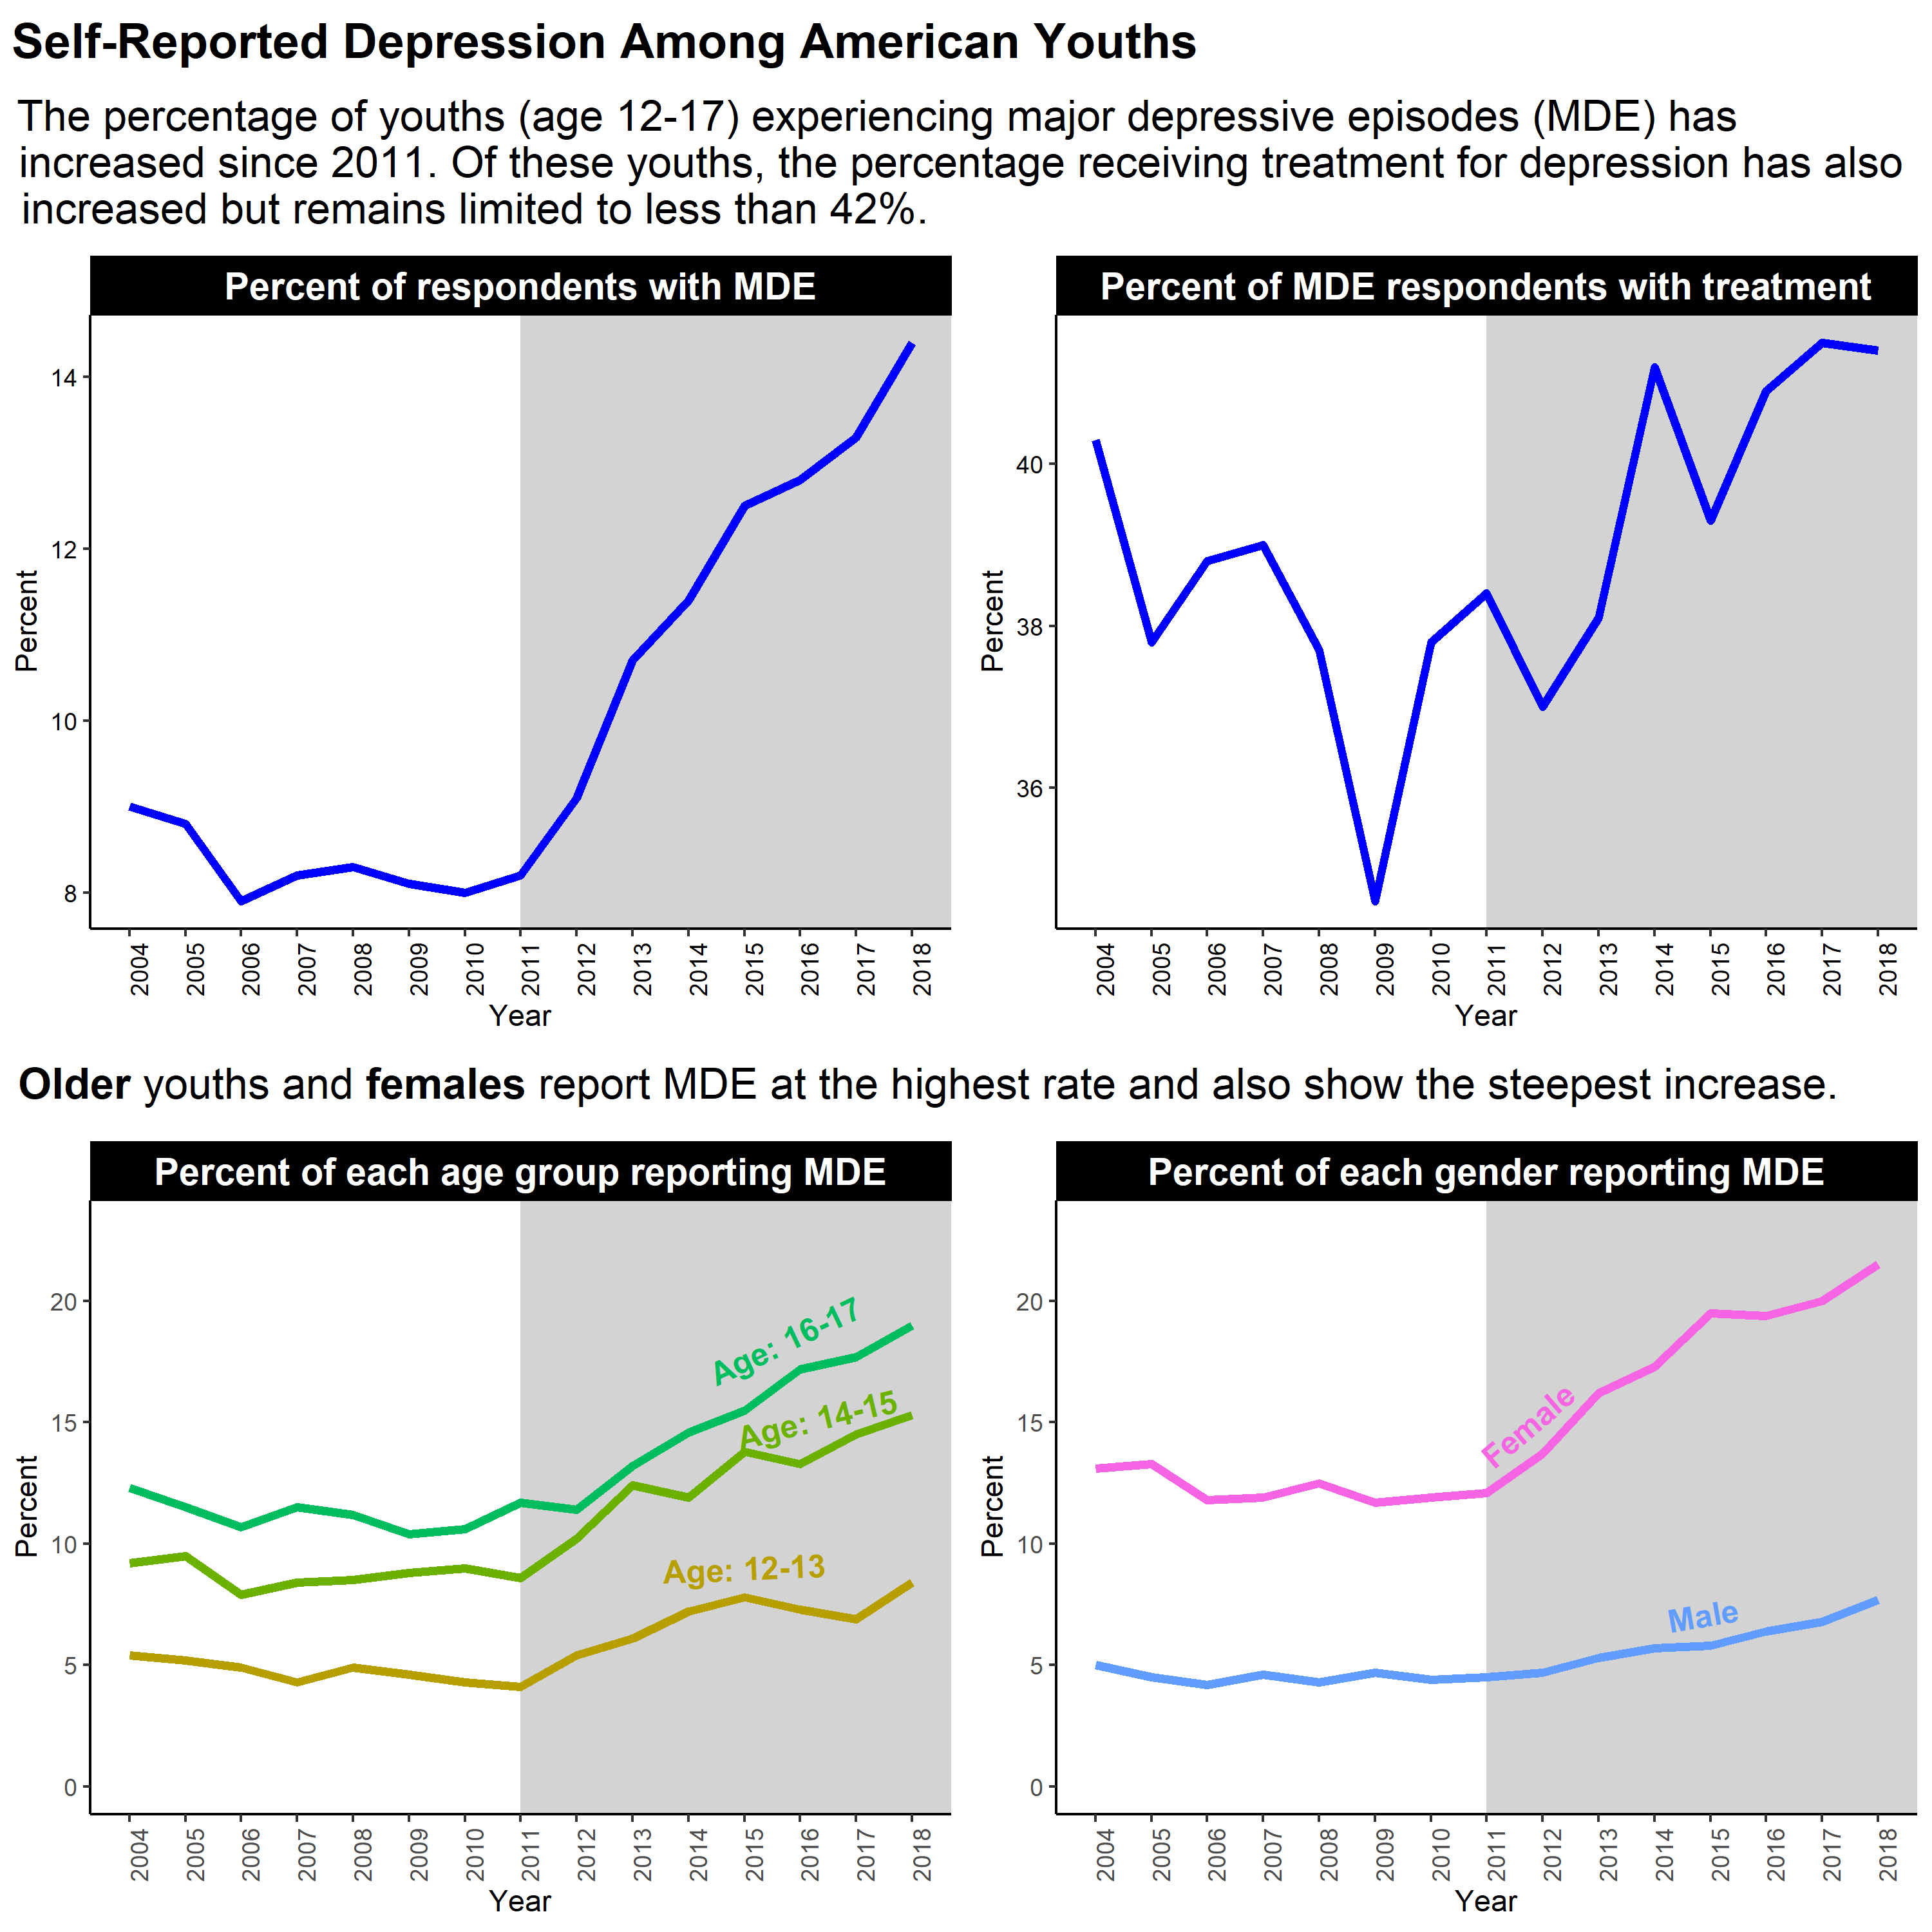
\includegraphics[width=800 px]{/Users/carriewright/Documents/GitHub/ocs-youth-mental-health-case-study/img/mainplot} \end{center}

\hypertarget{section-1}{%
\paragraph{}\label{section-1}}

\hypertarget{section-2}{%
\paragraph{}\label{section-2}}

\textbf{Disclaimer}: The purpose of the
\href{https://opencasestudies.github.io}{Open Case Studies} project is
\textbf{to demonstrate the use of various data science methods, tools,
and software in the context of messy, real-world data}. A given case
study does not cover all aspects of the research process, is not
claiming to be the most appropriate way to analyze a given data set, and
should not be used in the context of making policy decisions without
external consultation from scientific experts.

\hypertarget{section-3}{%
\paragraph{}\label{section-3}}

\hypertarget{section-4}{%
\paragraph{}\label{section-4}}

This work is licensed under the Creative Commons
Attribution-NonCommercial 3.0
\href{https://creativecommons.org/licenses/by-nc/3.0/us/}{(CC BY-NC
3.0)} United States License.

\hypertarget{section-5}{%
\paragraph{}\label{section-5}}

\hypertarget{section-6}{%
\paragraph{}\label{section-6}}

To cite this case study please use:

Wright, Carrie and Ontiveros, Michael and Jager, Leah and Taub, Margaret
and Hicks, Stephanie C. (2020).
\url{https://github.com/opencasestudies/ocs-bp-youth-mental-health}.
Mental Health of American Youth.

\hypertarget{section-7}{%
\paragraph{}\label{section-7}}

\hypertarget{section-8}{%
\paragraph{}\label{section-8}}

\textbf{Please be advised that the material in this case study describes
and discusses rates of suicide, as well as rates and symptoms of
depression.}

According to the
\href{https://www.nimh.nih.gov/health/publications/teen-depression/index.shtml}{National
Institute of Mental Health (NIMH)}:

If you are in crisis and need help, call this toll-free number for the
\textbf{National Suicide Prevention Lifeline (NSPL)}, available 24 hours
a day, every day: \textbf{1-800-273-TALK (8255)}. The service is
available to everyone. The deaf and hard of hearing can contact the
Lifeline via TTY at 1-800-799-4889. All calls are confidential. You can
also visit the Lifeline's website at
\url{www.suicidepreventionlifeline.org}.

The \textbf{Crisis Text Line} is another free, confidential resource
available 24 hours a day, seven days a week. Text ``HOME'' to
\textbf{741741} and a trained crisis counselor will respond to you with
support and information over text message. Visit
\url{www.crisistextline.org}.

Also see \href{https://www.mhanational.org/depression-teens-0}{here} for
more information about how to recognize and help youths experiencing
symptoms of depression.

\hypertarget{section-9}{%
\paragraph{}\label{section-9}}

To access the GitHub repository for this case study see here:
\url{https://github.com//opencasestudies/ocs-bp-youth-mental-health}.\\
This case study is part of a series of public health case studies for
the \href{https://americanhealth.jhu.edu/open-case-studies}{Bloomberg
American Health Initiative}.

\hypertarget{motivation}{%
\subsection{\texorpdfstring{\textbf{Motivation}}{Motivation}}\label{motivation}}

\begin{center}\rule{0.5\linewidth}{0.5pt}\end{center}

Rates of depression appear to have been increasing among American youths
since around 2010 according to a recent
\href{https://content.apa.org/record/2019-12578-001}{report}. A
\href{https://pubmed.ncbi.nlm.nih.gov/24285382/}{recent study} also
shows that youths appear to be seeking more care from mental health
services.

This case study will explore how rates of major depressive episodes have
changed since the early 2000s and across different youth subgroups (age,
gender, ethnicity). We also will explore how rates of treatment for
depression of youths have changed over time.

\begin{center}
\includegraphics[width=0.4\linewidth]{/Users/carriewright/Documents/GitHub/ocs-youth-mental-health-case-study/img/k-mitch-hodge-IqSaG9zv2e0-unsplash} \end{center}

{Photo by K. Mitch Hodge on Unsplash}

The major symptoms of a major depressive episode include:

\textbf{S}leep disorder (increased or decreased)\\
\textbf{I}nterest deficit (anhedonia)\\
\textbf{G}uilt (worthlessness, hopelessness, regret)\\
\textbf{E}nergy deficit\\
\textbf{C}oncentration deficit\\
\textbf{A}ppetite disorder (increased or decreased)\\
\textbf{P}sychomotor retardation or agitation\\
\textbf{S}uicidality

\hypertarget{source}{%
\subparagraph{\texorpdfstring{\href{https://www.icsi.org/guideline/depression/diagnose-and-characterize-major-depression-persistent-depressive-disorder-with-clinical-interview/}{{[}source{]}}}{{[}source{]}}}\label{source}}

\begin{center}
\includegraphics[width=0.8\linewidth]{/Users/carriewright/Documents/GitHub/ocs-youth-mental-health-case-study/img/depression-symptoms-and-treatment-768x768} \end{center}

\hypertarget{source-1}{%
\subparagraph{\texorpdfstring{\href{https://newmilfordcounselingcenter.com/depression-2/}{{[}source{]}}}{{[}source{]}}}\label{source-1}}

\begin{center}\rule{0.5\linewidth}{0.5pt}\end{center}

Click here to see the diagnostic requirements for a major depressive
episode (MSE) according to the
\href{https://en.wikipedia.org/wiki/DSM-5}{DSM 5}.

A. Five or more of the following symptoms have been present and
documented during the same two-week period and represent a change from
previous functioning; at least one of the symptoms is either (1)
depressed mood or (2) loss of interest or pleasure.

\textbf{Note}: Do not include symptoms that are clearly attributable to
another medical condition.

\begin{enumerate}
\def\labelenumi{\arabic{enumi}.}
\item
  Depressed mood most of the day, nearly every day, as indicated by
  either subjective report (e.g., feels sad, empty, hopeless) or
  observation made by others (e.g., appears tearful)
\item
  Markedly diminished interest or pleasure in all, or almost all,
  activities most of the day, nearly every day (as indicated by either
  subjective account or observation)
\item
  Significant weight loss when not dieting or weight gain (e.g., a
  change of more than 5\% of body weight in a month), or decrease or
  increase in appetite nearly every day
\item
  Insomnia or hypersomnia nearly every day
\item
  Psychomotor agitation or retardation nearly every day (observable by
  others, not merely subjective feelings of restlessness or being slowed
  down)
\item
  Fatigue or loss of energy nearly every day
\item
  Feelings of worthlessness or excessive or inappropriate guilt (which
  may be delusional) nearly every day (not merely self-reproach or guilt
  about being sick)
\item
  Diminished ability to think or concentrate, or indecisiveness, nearly
  every day (either by subjective account or as observed by others)
\item
  Recurrent thoughts of death (not just fear of dying), recurrent
  suicidal ideation without a specific plan, or a suicide attempt or a
  specific plan for committing suicide
\end{enumerate}

B. The symptoms do not meet criteria for a mixed episode.

C. The episode is not attributable to the physiological effects of a
substance or to another medical condition.

\textbf{Note}: Criteria A-C represent a major depressive episode.

\textbf{Note}: Responses to a significant loss (e.g., bereavement,
financial ruin, losses from a natural disaster, a serious medical
illness or disability) may include feelings of intense sadness,
rumination about the loss, insomnia, poor appetite and weight loss noted
in Criterion A, which may resemble a depressive episode. Although such
symptoms may be understandable or considered appropriate to the loss,
the presence of a major depressive episode in addition to the normal
response to a significant loss should also be carefully considered. This
decision inevitably requires the exercise of clinical judgment based on
the individual's history of and the cultural norms for the expression of
distress in the context of loss.

D. The occurrence of the major depressive episode is not better
explained by schizoaffective disorder, schizophrenia, schizophreniform
disorder, delusional disorder, or other specified and unspecified
schizophrenia spectrum and other psychotic disorders.

E. There has never been a manic episode or a hypomanic episode.

Note: This exclusion does not apply if all of the manic-like or
hypomanic-like episodes are substance-induced or are attributable to the
physiological effects of another medical condition.

\hypertarget{source-2}{%
\paragraph{\texorpdfstring{\href{https://www.icsi.org/guideline/depression/diagnose-and-characterize-major-depression-persistent-depressive-disorder-with-clinical-interview/}{{[}source{]}}}{{[}source{]}}}\label{source-2}}

\begin{center}\rule{0.5\linewidth}{0.5pt}\end{center}

This case study is motivated by the following two articles:

\hypertarget{section-10}{%
\paragraph{}\label{section-10}}

Twenge JM, Cooper AB, Joiner TE, Duffy ME, Binau SG. Age, period, and
cohort trends in mood disorder indicators and suicide-related outcomes
in a nationally representative dataset, 2005-2017. \emph{J Abnorm
Psychol}.128,3 (2019):185-199. \url{doi:10.1037/abn0000410}

Olfson, M., Blanco, C., Wang, S., Laje, G. \& Correll, C. U. National
Trends in the Mental Health Care of Children, Adolescents, and Adults by
Office-Based Physicians. \emph{JAMA Psychiatry}. 71, 81 (2014):81-90.
doi: 10.1001/jamapsychiatry.2013.3074.

\hypertarget{section-11}{%
\paragraph{}\label{section-11}}

The main findings of the first
\href{https://content.apa.org/record/2019-12578-001}{article} are:

\begin{quote}
Rates of major depressive episode in the last year increased 52\%
2005--2017 (from 8.7\% to 13.2\%) among adolescents aged 12 to 17 and
63\% 2009--2017 (from 8.1\% to 13.2\%) among young adults 18--25.
\end{quote}

\begin{quote}
Serious psychological distress in the last month and suicide-related
outcomes (suicidal ideation, plans, attempts, and deaths by suicide) in
the last year also increased among young adults 18--25 from 2008--2017
(with a 71\% increase in serious psychological distress), with less
consistent and weaker increases among adults ages 26 and over.
\end{quote}

\begin{quote}
Cultural trends contributing to an increase in mood disorders and
suicidal thoughts and behaviors since the mid-2000s, including the rise
of electronic communication and digital media and declines in sleep
duration, may have had a larger impact on younger people, creating a
cohort effect.
\end{quote}

While the main findings of the second
\href{https://pubmed.ncbi.nlm.nih.gov/24285382/}{article} are:

\begin{quote}
Compared with adult mental health care, the mental health care of young
people has increased more rapidly\ldots{}
\end{quote}

This means that the number of youths receiving mental health care has
increased faster than the number of adults receiving mental health care.

\begin{quote}
Between 1995-1998 and 2007-2010, visits resulting in mental disorder
diagnoses \ldots{} increased significantly faster for youths (from 7.78
to 15.30 visits) than for adults (from 23.23 to 28.48 visits)
(interaction: P \textless{} .001).
\end{quote}

\begin{quote}
Psychiatrist visits also increased significantly faster for youths (from
2.86 to 5.71 visits).
\end{quote}

\textbf{Summary}: While depression appears to be on the rise for youths,
youths also appear to be seeking more mental health care.

In this case study, we will be using data from the
\href{https://nsduhweb.rti.org/respweb/homepage.cfm}{National Survey on
Drug Use and Health (NSDUH)} related to treatment and major depressive
episode (MDE) rate to explore how trends in mental health have changed
over time and how different groups compare.

This data was also used in the first referenced article.

\hypertarget{main-questions}{%
\subsection{\texorpdfstring{\textbf{Main
Questions}}{Main Questions}}\label{main-questions}}

\begin{center}\rule{0.5\linewidth}{0.5pt}\end{center}

\hypertarget{section-12}{%
\paragraph{}\label{section-12}}

Our main questions:

\begin{enumerate}
\def\labelenumi{\arabic{enumi}.}
\tightlist
\item
  How have depression rates in American youth changed since 2004,
  according to the NSDUH data? How have rates differed between different
  youth subgroups (age, gender, ethnicity)?
\item
  Do mental health services appear to be reaching more youths? Again,
  how have rates differed between different youth subgroups (age,
  gender, ethnicity)?
\end{enumerate}

\hypertarget{section-13}{%
\paragraph{}\label{section-13}}

\hypertarget{learning-objectives}{%
\subsection{\texorpdfstring{\textbf{Learning
Objectives}}{Learning Objectives}}\label{learning-objectives}}

\begin{center}\rule{0.5\linewidth}{0.5pt}\end{center}

The skills, methods, and concepts that students will be familiar with by
the end of this case study are:

\textbf{Data Science Learning Objectives:}

\begin{enumerate}
\def\labelenumi{\arabic{enumi}.}
\tightlist
\item
  Scrape data directly from a website (\texttt{rvest})\\
\item
  Subset and filter data (\texttt{dplyr})\\
\item
  Write functions to wrangle data repetitively\\
\item
  Work with character strings (\texttt{stringr})\\
\item
  Reshape data into different formats (\texttt{tidyr})\\
\item
  Data visualizations (\texttt{ggplot2}) with labels
  (\texttt{directlabels}) and facets for different groups\\
\item
  Combine multiple plots (\texttt{cowplot})\\
\item
  Optional: Create an animated gif (\texttt{magick})
\end{enumerate}

\textbf{Statistical Learning Objectives:}

\begin{enumerate}
\def\labelenumi{\arabic{enumi}.}
\tightlist
\item
  Discuss the impact of self-reporting bias on survey responses\\
\item
  Define and create a contingency table\\
\item
  Implementation of a chi-squared test for independence\\
\item
  Interpretation of a chi-squared test for independence
\end{enumerate}

In this case study, we will especially focus on using packages and
functions from the
\href{https://www.tidyverse.org/}{\texttt{Tidyverse}}, such as
\href{https://github.com/tidyverse/rvest}{\texttt{rvest}}. The tidyverse
is a library of packages created by RStudio. While some students may be
familiar with previous R programming packages, these packages make data
science in R more legible and intuitive.

\begin{center}\rule{0.5\linewidth}{0.5pt}\end{center}

We will begin by loading the packages that we will need:

\begin{Shaded}
\begin{Highlighting}[]
\KeywordTok{library}\NormalTok{(here)}
\KeywordTok{library}\NormalTok{(rvest)}
\KeywordTok{library}\NormalTok{(dplyr)}
\KeywordTok{library}\NormalTok{(magrittr)}
\KeywordTok{library}\NormalTok{(stringr)}
\KeywordTok{library}\NormalTok{(tidyr)}
\KeywordTok{library}\NormalTok{(tibble)}
\KeywordTok{library}\NormalTok{(purrr)}
\KeywordTok{library}\NormalTok{(ggplot2)}
\KeywordTok{library}\NormalTok{(directlabels)}
\KeywordTok{library}\NormalTok{(scales)}
\KeywordTok{library}\NormalTok{(forcats)}
\KeywordTok{library}\NormalTok{(ggthemes)}
\KeywordTok{library}\NormalTok{(cowplot)}
\end{Highlighting}
\end{Shaded}

\textbf{Packages used in this case study:}

\begin{longtable}[]{@{}ll@{}}
\toprule
\begin{minipage}[b]{0.41\columnwidth}\raggedright
Package\strut
\end{minipage} & \begin{minipage}[b]{0.53\columnwidth}\raggedright
Use in this case study\strut
\end{minipage}\tabularnewline
\midrule
\endhead
\begin{minipage}[t]{0.41\columnwidth}\raggedright
\href{https://github.com/jennybc/here_here}{here}\strut
\end{minipage} & \begin{minipage}[t]{0.53\columnwidth}\raggedright
to easily load and save data\strut
\end{minipage}\tabularnewline
\begin{minipage}[t]{0.41\columnwidth}\raggedright
\href{https://github.com/tidyverse/rvest}{rvest}\strut
\end{minipage} & \begin{minipage}[t]{0.53\columnwidth}\raggedright
to scrape web pages\strut
\end{minipage}\tabularnewline
\begin{minipage}[t]{0.41\columnwidth}\raggedright
\href{https://dplyr.tidyverse.org/}{dplyr}\strut
\end{minipage} & \begin{minipage}[t]{0.53\columnwidth}\raggedright
to subset and filter the data for specific groups, to replace specific
values with \texttt{NA}, rename variables, and perform functions on
multiple variables\strut
\end{minipage}\tabularnewline
\begin{minipage}[t]{0.41\columnwidth}\raggedright
\href{https://magrittr.tidyverse.org/}{magrittr}\strut
\end{minipage} & \begin{minipage}[t]{0.53\columnwidth}\raggedright
to use and reassign data objects using the \%\textless\textgreater\%pipe
operator\strut
\end{minipage}\tabularnewline
\begin{minipage}[t]{0.41\columnwidth}\raggedright
\href{https://stringr.tidyverse.org/}{stringr}\strut
\end{minipage} & \begin{minipage}[t]{0.53\columnwidth}\raggedright
to manipulate strings\strut
\end{minipage}\tabularnewline
\begin{minipage}[t]{0.41\columnwidth}\raggedright
\href{https://tidyr.tidyverse.org/}{tidyr}\strut
\end{minipage} & \begin{minipage}[t]{0.53\columnwidth}\raggedright
to change the shape or format of tibbles to wide and long\strut
\end{minipage}\tabularnewline
\begin{minipage}[t]{0.41\columnwidth}\raggedright
\href{https://tibble.tidyverse.org/}{tibble}\strut
\end{minipage} & \begin{minipage}[t]{0.53\columnwidth}\raggedright
to create tibbles and convert values of a column to row names\strut
\end{minipage}\tabularnewline
\begin{minipage}[t]{0.41\columnwidth}\raggedright
\href{https://purrr.tidyverse.org/}{purrr}\strut
\end{minipage} & \begin{minipage}[t]{0.53\columnwidth}\raggedright
to apply a function to each column of a tibble or each tibble in a
list\strut
\end{minipage}\tabularnewline
\begin{minipage}[t]{0.41\columnwidth}\raggedright
\href{https://ggplot2.tidyverse.org/}{ggplot2}\strut
\end{minipage} & \begin{minipage}[t]{0.53\columnwidth}\raggedright
to create plots\strut
\end{minipage}\tabularnewline
\begin{minipage}[t]{0.41\columnwidth}\raggedright
\href{http://directlabels.r-forge.r-project.org/docs/index.html}{directlabels}\strut
\end{minipage} & \begin{minipage}[t]{0.53\columnwidth}\raggedright
to add labels directly to lines in plots\strut
\end{minipage}\tabularnewline
\begin{minipage}[t]{0.41\columnwidth}\raggedright
\href{https://cran.r-project.org/web/packages/scales/scales.pdf}{scales}\strut
\end{minipage} & \begin{minipage}[t]{0.53\columnwidth}\raggedright
to get the current linetype options\strut
\end{minipage}\tabularnewline
\begin{minipage}[t]{0.41\columnwidth}\raggedright
\href{https://forcats.tidyverse.org/}{forcats}\strut
\end{minipage} & \begin{minipage}[t]{0.53\columnwidth}\raggedright
to reorder factor for plot\strut
\end{minipage}\tabularnewline
\begin{minipage}[t]{0.41\columnwidth}\raggedright
\href{https://cran.r-project.org/web/packages/ggthemes/ggthemes.pdf}{ggthemes}\strut
\end{minipage} & \begin{minipage}[t]{0.53\columnwidth}\raggedright
to create a plot to see what the different linetypes look like\strut
\end{minipage}\tabularnewline
\begin{minipage}[t]{0.41\columnwidth}\raggedright
\href{https://cran.r-project.org/web/packages/cowplot/vignettes/introduction.html}{cowplot}\strut
\end{minipage} & \begin{minipage}[t]{0.53\columnwidth}\raggedright
to combine plots together\strut
\end{minipage}\tabularnewline
\bottomrule
\end{longtable}

The first time we use a function, we will use the \texttt{::} to
indicate which package we are using. Unless we have overlapping function
names, this is not necessary, but we will include it here to be
informative about where the functions we will use come from.

\hypertarget{context}{%
\subsection{\texorpdfstring{\textbf{Context}}{Context}}\label{context}}

\begin{center}\rule{0.5\linewidth}{0.5pt}\end{center}

To motivate the examination of the mental health of American youths, we
begin by exploring the rate of suicide in the United States (US).
According to the CDC the rate of suicide has increased for both genders.

\hypertarget{source-3}{%
\subparagraph{\texorpdfstring{\href{https://www.cdc.gov/nchs/products/databriefs/db309.htm}{{[}source{]}}}{{[}source{]}}}\label{source-3}}

While suicide does appear to be increasing among youths it also appears
to be increasing among most age groups in the US over the past decade
and a half for both females and males:

\includegraphics[width=0.5\linewidth]{https://www.cdc.gov/nchs/images/databriefs/301-350/db309_fig2}
\includegraphics[width=0.5\linewidth]{https://www.cdc.gov/nchs/images/databriefs/301-350/db309_fig3}

\hypertarget{source-4}{%
\subparagraph{\texorpdfstring{\href{https://www.cdc.gov/nchs/products/databriefs/db309.htm}{{[}source{]}}}{{[}source{]}}}\label{source-4}}

According to the
\href{https://www.cdc.gov/nchs/products/databriefs/db309.htm}{CDC}:

\begin{quote}
Since 2008, suicide has ranked as the 10th leading cause of death for
\textbf{all ages} in the United States.
\end{quote}

\begin{center}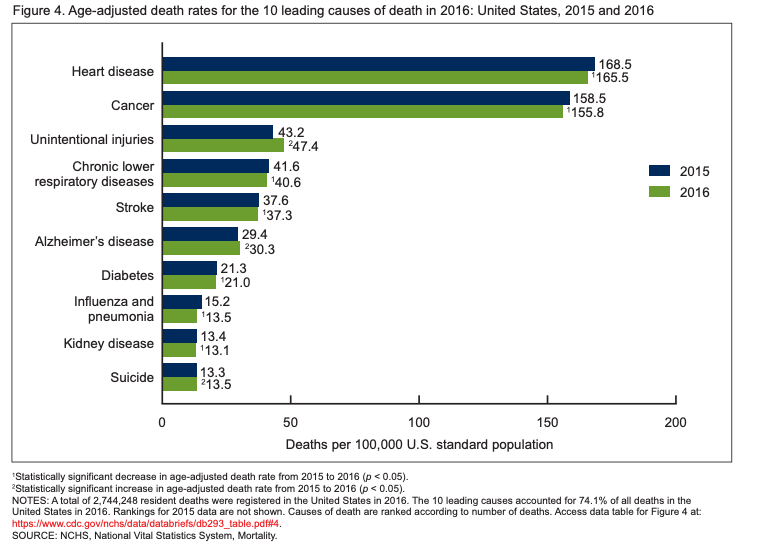
\includegraphics[width=800px]{/Users/carriewright/Documents/GitHub/ocs-youth-mental-health-case-study/img/mortality} \end{center}

\hypertarget{source-5}{%
\subparagraph{\texorpdfstring{\href{https://www.cdc.gov/nchs/data/databriefs/db293.pdf}{{[}source{]}}}{{[}source{]}}}\label{source-5}}

Furthermore, according to the
\href{https://www.cdc.gov/nchs/products/databriefs/db309.htm}{CDC}:

\begin{quote}
In 2016, suicide became the \textbf{second leading cause of death} among
youths.
\end{quote}

\textbf{So although suicide is on the rise for most age groups, suicide
is one of the top \emph{two} contributors to death for youths.}

Thus, this warrants further examination of the mental health of American
youths.

\begin{center}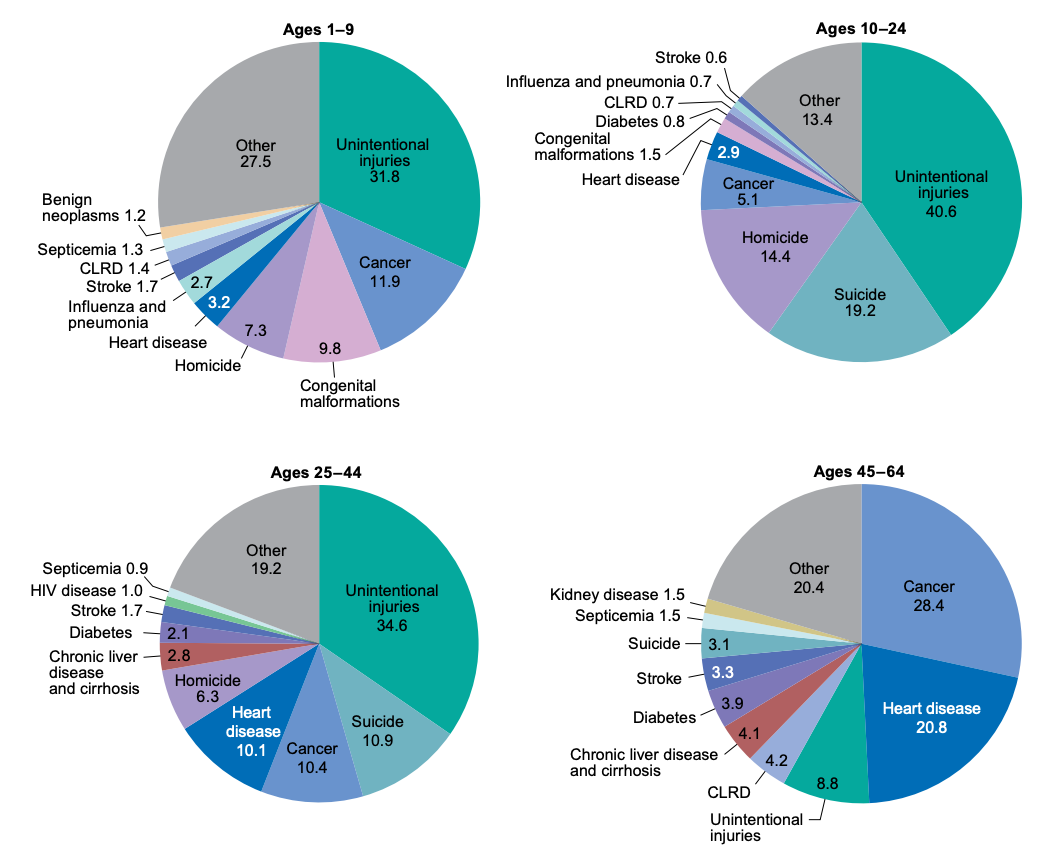
\includegraphics[width=800px]{/Users/carriewright/Documents/GitHub/ocs-youth-mental-health-case-study/img/mortality_age} \end{center}

\hypertarget{source-6}{%
\subparagraph{\texorpdfstring{\href{https://www.cdc.gov/nchs/data/nvsr/nvsr68/nvsr68_06-508.pdf}{{[}source{]}}}{{[}source{]}}}\label{source-6}}

Historically, suicide rates were much higher before 1950, however, we
are seeing an increase in the last 20 years.

\begin{center}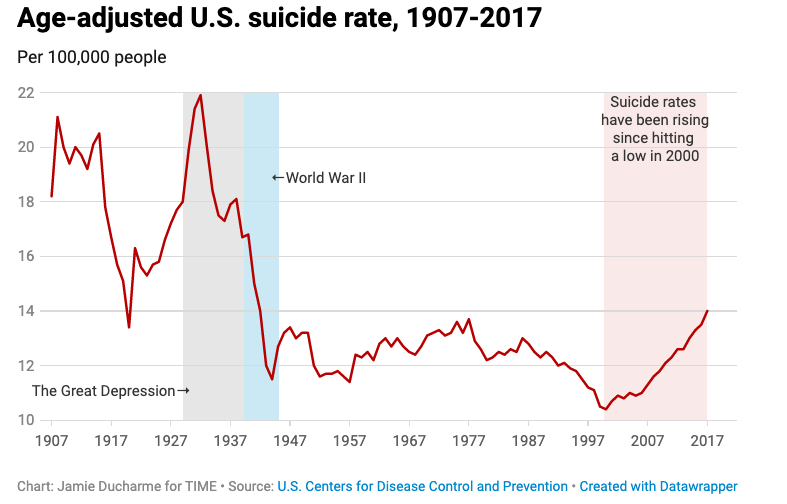
\includegraphics[width=800px]{/Users/carriewright/Documents/GitHub/ocs-youth-mental-health-case-study/img/suicide} \end{center}

\hypertarget{source-7}{%
\subparagraph{\texorpdfstring{\href{https://time.com/5609124/us-suicide-rate-increase/}{{[}source{]}}}{{[}source{]}}}\label{source-7}}

Besides the US,
\href{https://academic.oup.com/ije/article/48/5/1650/5366210}{other
countries} are also experiencing increased rates of depression in
youths.

See
\href{https://apps.who.int/iris/bitstream/handle/10665/254610/WHO-MSD-MER-2017.2-eng.pdf;jsessionid=E44360055DD83EAC472AA40C2853DBFA?sequence=1}{this
report} from the World Health Organization (WHO) about rates of
depression in other countries.

See \href{https://www.ncbi.nlm.nih.gov/pmc/articles/PMC3330161/}{here}
for an interesting discussion about what may be causing increased
depression rates.

\hypertarget{limitations}{%
\subsection{\texorpdfstring{\textbf{Limitations}}{Limitations}}\label{limitations}}

\begin{center}\rule{0.5\linewidth}{0.5pt}\end{center}

There are some important considerations regarding this data analysis to
keep in mind:

\begin{enumerate}
\def\labelenumi{\arabic{enumi}.}
\item
  The data that we will use come from a survey and are therefore values
  from a sample that estimate that of the true population. In our
  statistical analysis we use these sample values as if they are
  population estimates (because this is all we have access to). Thus,
  our results are not necessarily indicative of population differences.
\item
  Furthermore, the sampling mechanism utilized for the survey can
  introduce
  \href{https://en.wikipedia.org/wiki/Selection_bias?oldformat=true}{selection
  bias} in cases where the the
  \href{https://en.wikipedia.org/wiki/Sampling_(statistics)?oldformat=true}{sampling
  methods do not produce a representative sample}.
\item
  Data are collected from human participants; this presents the
  \emph{potential} for information bias, as there is the
  \emph{potential} that participants in the
  \href{https://en.wikipedia.org/wiki/Sampling_frame?oldformat=true}{sampling
  frame} may for a variety of reasons report inaccurate information.
\item
  Data about certain group
  \href{https://www.vox.com/the-highlight/2019/5/20/18542843/intersectionality-conservatism-law-race-gender-discrimination}{intersections}
  (meaning for example individuals of a particular gender and ethnicity)
  or particular groups in general such as specific ethnicities or gender
  or sexual identity groups such as LGBTQIA+
  (lesbian/gay/bisexual/transgender/queer and questioning) or non-binary
  gender populations is unfortunately not available in the data used in
  this analysis and in most research about this topic.
\end{enumerate}

Note: While
\href{https://www.who.int/genomics/gender/en/index1.html}{gender and
sex} are not actually binary, the data used in this analysis
unfortunately only contains information for groups of individuals who
self-reported as male or female. We also acknowledge that unfortunately
not all ethnicities or group intersections are represented in the data
either. More research should be devoted to collecting data about the
mental health of these groups.

\hypertarget{what-are-the-data}{%
\subsection{\texorpdfstring{\textbf{What are the
data?}}{What are the data?}}\label{what-are-the-data}}

\begin{center}\rule{0.5\linewidth}{0.5pt}\end{center}

We will be using data from the
\href{https://nsduhweb.rti.org/respweb/homepage.cfm}{National Survey on
Drug Use and Health (NSDUH)} which is directed by the
\href{https://www.samhsa.gov/}{Substance Abuse and Mental Health
Services Administration (SAMHSA)}, an agency in the
\href{https://www.hhs.gov/}{U.S. Department of Health and Human Services
(DHHS)}.

This survey started in 1971 and is conducted annually in all 50 states
and the District of Columbia. Approximately 70,000 people (ages 12 and
up) are interviewed each year about health-related issues. Only
civilian, non-institutionalized individuals are included. Households are
randomly selected and then a professional interviewer visits the
addresses and asks one or two of the residents to interview. The
interviewer brings a laptop with them that the participants use to fill
out the survey, which typically takes an hour to complete. If a
participant chooses to participate they receive \$30 in cash. All
collected information is confidential and is used for disease
surveillance and to guide public policy particularly focused on drug and
alcohol use as well as mental health. See
\href{https://nsduhweb.rti.org/respweb/about_nsduh.html}{here} for more
details about the survey.

The data are made available publicly online on the
\href{https://datafiles.samhsa.gov/}{Substance Abuse \& Mental Health
Data Archive}.

\begin{center}
\includegraphics[width=1\linewidth]{/Users/carriewright/Documents/GitHub/ocs-youth-mental-health-case-study/img/nsudh_screenshot_webpage} \end{center}

On the
\href{https://www.samhsa.gov/data/sites/default/files/cbhsq-reports/NSDUHDetailedTabs2018R2/NSDUHDetTabsSect11pe2018.htm}{website}
with the survey data, you can see that the results are displayed in many
tables. Importantly, there is no obvious way to download the data
directly from this particular website.

\begin{center}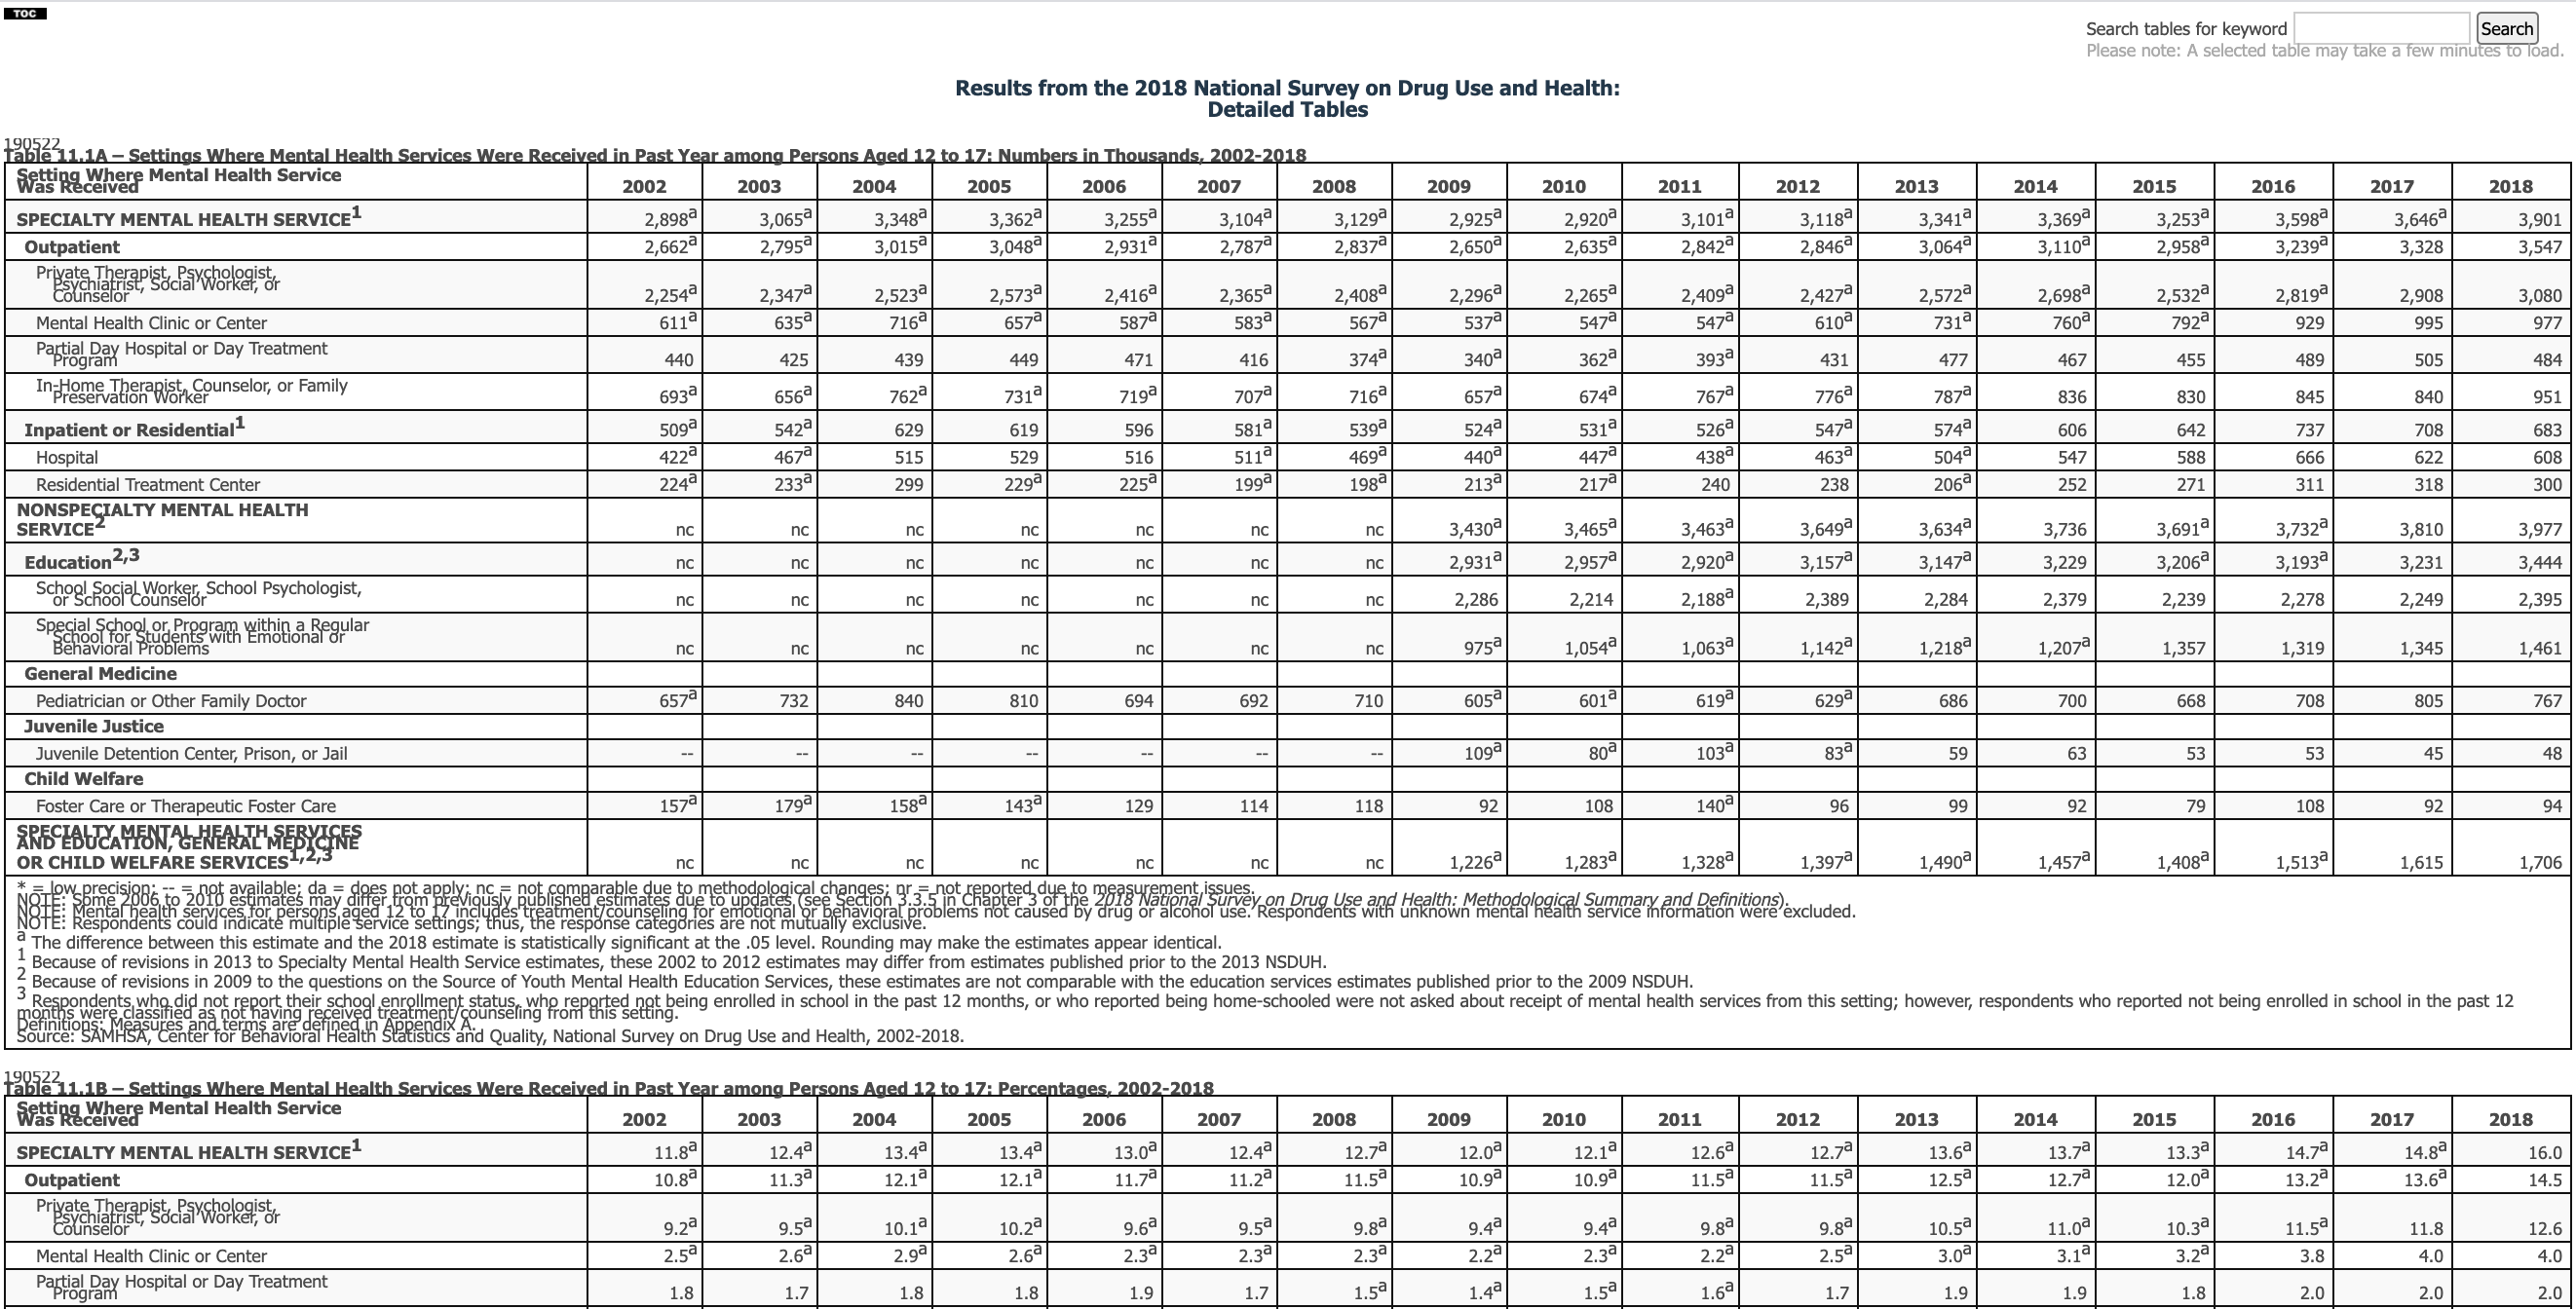
\includegraphics[width=1\linewidth]{/Users/carriewright/Documents/GitHub/ocs-youth-mental-health-case-study/img/website_overview} \end{center}

If you click on the TOC button on the far left upper corner, you will be
directed to another
\href{https://www.samhsa.gov/data/sites/default/files/cbhsq-reports/NSDUHDetailedTabs2018R2/NSDUHDetailedTabsTOC2018.htm\#toc}{website},
where a large
\href{https://www.samhsa.gov/data/sites/default/files/cbhsq-reports/NSDUHDetailedTabs2018R2/NSDUHDetailedTabs2018.pdf}{pdf
document} containing all of the results can be downloaded.

We are interested in investigating how depression rates have changed and
how youths are interacting with mental health services. Thus, the
following tables are of interest to us:

\begin{longtable}[]{@{}ll@{}}
\toprule
\begin{minipage}[b]{0.18\columnwidth}\raggedright
Table\strut
\end{minipage} & \begin{minipage}[b]{0.76\columnwidth}\raggedright
Details\strut
\end{minipage}\tabularnewline
\midrule
\endhead
\begin{minipage}[t]{0.18\columnwidth}\raggedright
Table 11.1A\strut
\end{minipage} & \begin{minipage}[t]{0.76\columnwidth}\raggedright
Settings Where Mental Health Services Were Received in Past Year among
Persons Aged 12 to 17: Numbers in Thousands, 2002-2018\strut
\end{minipage}\tabularnewline
\begin{minipage}[t]{0.18\columnwidth}\raggedright
Table 11.1B\strut
\end{minipage} & \begin{minipage}[t]{0.76\columnwidth}\raggedright
Settings Where Mental Health Services Were Received in Past Year among
Persons Aged 12 to 17: Percentages, 2002-2018\strut
\end{minipage}\tabularnewline
\begin{minipage}[t]{0.18\columnwidth}\raggedright
Table 11.2A\strut
\end{minipage} & \begin{minipage}[t]{0.76\columnwidth}\raggedright
Major Depressive Episode in Past Year among Persons Aged 12 to 17, by
Demographic Characteristics: Numbers in Thousands, 2004-2018\strut
\end{minipage}\tabularnewline
\begin{minipage}[t]{0.18\columnwidth}\raggedright
Table 11.2B\strut
\end{minipage} & \begin{minipage}[t]{0.76\columnwidth}\raggedright
Major Depressive Episode in Past Year among Persons Aged 12 to 17, by
Demographic Characteristics: Percentages, 2004-2018\strut
\end{minipage}\tabularnewline
\begin{minipage}[t]{0.18\columnwidth}\raggedright
Table 11.3A\strut
\end{minipage} & \begin{minipage}[t]{0.76\columnwidth}\raggedright
Major Depressive Episode with Severe Impairment in Past Year among
Persons Aged 12 to 17, by Demographic Characteristics: Numbers in
Thousands, 2006-2018\strut
\end{minipage}\tabularnewline
\begin{minipage}[t]{0.18\columnwidth}\raggedright
Table 11.3B\strut
\end{minipage} & \begin{minipage}[t]{0.76\columnwidth}\raggedright
Major Depressive Episode with Severe Impairment in Past Year among
Persons Aged 12 to 17, by Demographic Characteristics: Percentages,
2006-2018\strut
\end{minipage}\tabularnewline
\begin{minipage}[t]{0.18\columnwidth}\raggedright
Table 11.4A\strut
\end{minipage} & \begin{minipage}[t]{0.76\columnwidth}\raggedright
Receipt of Treatment for Depression in Past Year among Persons Aged 12
to 17 with Major Depressive Episode in Past Year, by Demographic
Characteristics: Numbers in Thousands, 2004-2018\strut
\end{minipage}\tabularnewline
\begin{minipage}[t]{0.18\columnwidth}\raggedright
Table 11.4B\strut
\end{minipage} & \begin{minipage}[t]{0.76\columnwidth}\raggedright
Receipt of Treatment for Depression in Past Year among Persons Aged 12
to 17 with Major Depressive Episode in Past Year, by Demographic
Characteristics: Percentages, 2004-2018\strut
\end{minipage}\tabularnewline
\bottomrule
\end{longtable}

Our goal is to bring these data into R so we can explore them.

\begin{center}\rule{0.5\linewidth}{0.5pt}\end{center}

Click here for the NSDUH defines a major depressive episode (MDE)

According to the
\href{https://www.samhsa.gov/data/sites/default/files/cbhsq-reports/NSDUHNationalFindingsReport2018/NSDUHNationalFindingsReport2018.pdf}{NSDUH
2018 report}

\begin{quote}
Respondents were defined as having had an MDE in the past 12 months if
they had at least one period of 2 weeks or longer in the past year when
they experienced a depressed mood or loss of interest or pleasure in
daily activities, accompanied by problems with sleeping, eating, energy,
concentration, or self-worth. The MDE questions are based on diagnostic
criteria from DSM-5. Some of the wordings of the depression questions
for adolescents aged 12 to 17 and adults aged 18 or older differed
slightly to make the questions more developmentally appropriate for
adolescents.
\end{quote}

\begin{quote}
Adolescents were defined as having an MDE with severe impairment if
their depression caused severe problems with their ability to do chores
at home, do well at work or school, get along with their family, or have
a social life.
\end{quote}

\begin{center}\rule{0.5\linewidth}{0.5pt}\end{center}

\hypertarget{data-import}{%
\subsection{\texorpdfstring{\textbf{Data
Import}}{Data Import}}\label{data-import}}

\begin{center}\rule{0.5\linewidth}{0.5pt}\end{center}

Data are often made available online. Sometimes, the data we are
interested in is made available for download on a web page as a
delimited text file or an excel file. However, sometimes data are not
made available in this manner, such as the
\href{https://www.samhsa.gov/data/sites/default/files/cbhsq-reports/NSDUHDetailedTabs2018R2/NSDUHDetTabsSect11pe2018.htm}{NSDUH
survey data}.

How do we proceed in this scenario?

We can manually copy each cell of data; however, this process is often
inefficient, subject to error, and not reproducible. Say we wanted to
run an analysis next year on the next years data and it happens to be
formatted in the same way.

Alternatively, we could use \texttt{R} to scrape the data from the web!

Formally,
\href{https://en.wikipedia.org/wiki/Web_scraping?oldformat=true}{web
scraping} is the process of extracting data from a webpage. Let's learn
how to do this for our case study.

\hypertarget{basic-steps-of-web-scraping}{%
\subsubsection{\texorpdfstring{\textbf{Basic steps of web
scraping}}{Basic steps of web scraping}}\label{basic-steps-of-web-scraping}}

\begin{center}\rule{0.5\linewidth}{0.5pt}\end{center}

There are two main steps to web scraping:

\begin{enumerate}
\def\labelenumi{\arabic{enumi}.}
\item
  Identify \textbf{location} of data on the webpage that will be
  scraped.
\item
  Save the webpage \textbf{element} to an R \textbf{object}.
\end{enumerate}

We accomplish STEP 1 with our web browser.

We accomplish STEP 2 in the \texttt{R} programming environment.

The \textbf{location} of the data on the webpage that will be scraped
can be identified using a language called
\href{https://en.wikipedia.org/wiki/XPath}{XPath}, which is short for
XML Path Language. It is used to identify pieces (in this case called
\textbf{nodes}) of a document written in the
\href{https://en.wikipedia.org/wiki/XML}{XML} language.
\href{https://en.wikipedia.org/wiki/XML}{XML} which is short for
Extensible Markup Language is frequently used for documents on the
internet, similar to \href{https://en.wikipedia.org/wiki/HTML}{HTML}.
One of the
\href{https://techdifferences.com/difference-between-xml-and-html.html}{major
differences} between these two is that HTML does not provide structural
information, while XML does. This structural information can be used to
parse documents so that we can scrape only the data that we are
interested in from a website.

\hypertarget{section-14}{%
\paragraph{}\label{section-14}}

Additional resources for web scraping:

\begin{itemize}
\tightlist
\item
  \href{https://rstudio-pubs-static.s3.amazonaws.com/266430_f3fd4660b2744751ab144aa130768a06.html}{Vignette}
\item
  \href{http://blog.corynissen.com/2015/01/using-rvest-to-scrape-html-table.html}{Blog}
\item
  \href{http://research.libd.org/rstatsclub/post/introduction-to-scraping-and-wranging-tables-from-research-articles/\#.Xw878ZNKhQJ}{Blog}
\item
  \href{https://cran.r-project.org/web/packages/rvest/vignettes/selectorgadget.html}{Selectorgadget
  Tool}
\end{itemize}

\hypertarget{section-15}{%
\paragraph{}\label{section-15}}

\hypertarget{the-rvest-package}{%
\subsubsection{\texorpdfstring{\textbf{The \texttt{rvest}
package}}{The rvest package}}\label{the-rvest-package}}

\begin{center}\rule{0.5\linewidth}{0.5pt}\end{center}

In this case study, we will scrape data from the tables on the
\href{https://www.samhsa.gov/data/sites/default/files/cbhsq-reports/NSDUHDetailedTabs2018R2/NSDUHDetTabsSect11pe2018.htm}{NSDUH
survey} website.

Note that these data are available in a large PDF with all the results
by year if you wish to use the data from this particular source.

One option to import the data would be to import the PDF. However it is
not easy to find this PDF and it would be difficult and time consuming
to find our tables of interest and to extract our data of interest from
the pdf. However, if one wanted to do this, say if the tables were not
available online, they could use the \texttt{pdftools} package. See this
other \href{https://www.opencasestudies.org/ocs-bp-diet/}{case study}
and this other
\href{https://www.opencasestudies.org/ocs-bp-youth-disconnection/}{case
study} for two methods to work with PDFs.

Another option could be to copy and paste the data from the website to
another file that we would also need to import. But this would not be as
efficient or reproducible and might result in errors.

Alternatively, we will use the \texttt{rvest} package to
\href{https://en.wikipedia.org/wiki/Web_scraping?oldformat=true}{scrape}
the data directly from the tables on the website.

Assuming the data next year would be displayed in a similar manner, this
could allow us to simply modify our code based on the url for the data
next year to run the same analysis on the data easily.

However, it is important to keep in mind that one downside of scraping
the data directly from the web, is that the website could change - this
can be a good thing if the website adds additional data and keeps the
same formatting. This would allow us to get additional data very easily.
However, if the website changes formatting then this would require that
we update our code.

\hypertarget{scraping-tables-into-r}{%
\subsubsection{\texorpdfstring{\textbf{Scraping tables into
R}}{Scraping tables into R}}\label{scraping-tables-into-r}}

\begin{center}\rule{0.5\linewidth}{0.5pt}\end{center}

The two web scraping steps for these tables can be broken down even
further:

\begin{enumerate}
\def\labelenumi{\arabic{enumi}.}
\item
  Identify location of data that will be scraped

  \begin{itemize}
  \tightlist
  \item
    right-click to inspect element (webpage)
  \item
    hover pointer over components of element (webpage) until the data
    has been found
  \item
    copy XPath of data sought
  \end{itemize}
\item
  Save webpage element to an object in R

  \begin{itemize}
  \tightlist
  \item
    import html code for the webpage
  \item
    extract pieces of HTML documents (webpage) using XPath
  \item
    parse the extracted data into a data frame
  \end{itemize}
\end{enumerate}

Below is a animated overview of the process.

Click here if you want to see how this animation was made!

First the images need to be imported into R using the
\texttt{image\_read} function of the \texttt{magick} package.

\begin{Shaded}
\begin{Highlighting}[]
\NormalTok{step1 <-}\StringTok{ }\NormalTok{magick}\OperatorTok{::}\KeywordTok{image_read}\NormalTok{(here}\OperatorTok{::}\KeywordTok{here}\NormalTok{(}\StringTok{"img"}\NormalTok{, }\StringTok{"webpage_screenshot.png"}\NormalTok{))}
\NormalTok{step2 <-}\StringTok{ }\KeywordTok{image_read}\NormalTok{(here}\OperatorTok{::}\KeywordTok{here}\NormalTok{(}\StringTok{"img"}\NormalTok{, }\StringTok{"table_screenshot_inspect.png"}\NormalTok{))}
\NormalTok{step3 <-}\StringTok{ }\KeywordTok{image_read}\NormalTok{(here}\OperatorTok{::}\KeywordTok{here}\NormalTok{(}\StringTok{"img"}\NormalTok{, }\StringTok{"table_screenshot_inspect_table.png"}\NormalTok{))}
\NormalTok{step4 <-}\StringTok{ }\KeywordTok{image_read}\NormalTok{(here}\OperatorTok{::}\KeywordTok{here}\NormalTok{(}\StringTok{"img"}\NormalTok{, }\StringTok{"table_screenshot_inspect_table_xpath.png"}\NormalTok{))}
\NormalTok{step5 <-}\StringTok{ }\KeywordTok{image_read}\NormalTok{(here}\OperatorTok{::}\KeywordTok{here}\NormalTok{(}\StringTok{"img"}\NormalTok{, }\StringTok{"table_screenshot_xpath_copy_r.png"}\NormalTok{))}
\NormalTok{step5_zoom <-}\StringTok{ }\KeywordTok{image_read}\NormalTok{(here}\OperatorTok{::}\KeywordTok{here}\NormalTok{(}\StringTok{"img"}\NormalTok{, }\StringTok{"table_screenshot_xpath_copy_r_zoom.png"}\NormalTok{))}
\end{Highlighting}
\end{Shaded}

The last image is smaller than the others, to get a sense of the size we
can use the \texttt{image\_info()} function of the \texttt{magick}
package.

\begin{Shaded}
\begin{Highlighting}[]
\NormalTok{step5}
\end{Highlighting}
\end{Shaded}

\begin{center}\includegraphics[width=0.9\linewidth]{index_files/figure-latex/unnamed-chunk-13-1} \end{center}

\begin{Shaded}
\begin{Highlighting}[]
\NormalTok{step5_zoom}
\end{Highlighting}
\end{Shaded}

\begin{center}\includegraphics[width=0.9\linewidth]{index_files/figure-latex/unnamed-chunk-13-2} \end{center}

\begin{Shaded}
\begin{Highlighting}[]
\KeywordTok{image_info}\NormalTok{(step5)}
\end{Highlighting}
\end{Shaded}

\begin{verbatim}
# A tibble: 1 x 7
  format width height colorspace matte filesize density
  <chr>  <int>  <int> <chr>      <lgl>    <int> <chr>  
1 PNG     1440    900 sRGB       TRUE    306274 72x72  
\end{verbatim}

\begin{Shaded}
\begin{Highlighting}[]
\KeywordTok{image_info}\NormalTok{(step5_zoom)}
\end{Highlighting}
\end{Shaded}

\begin{verbatim}
# A tibble: 1 x 7
  format width height colorspace matte filesize density
  <chr>  <int>  <int> <chr>      <lgl>    <int> <chr>  
1 PNG      869    231 sRGB       TRUE     57559 72x72  
\end{verbatim}

First let's re-size the second image to make it a bit larger using the
\texttt{image\_resize()} function of the \texttt{magick} package. We
will re-size the width to be the same as the previous image width and
keep the aspect ratio for the height by using ``1440x''. If we wanted to
just do the same for height we would use ``x900''.

\begin{Shaded}
\begin{Highlighting}[]
\NormalTok{step5_zoom <-}\StringTok{ }\KeywordTok{image_resize}\NormalTok{(step5_zoom,  }\StringTok{"1440x"}\NormalTok{)}
\NormalTok{step5_zoom}
\end{Highlighting}
\end{Shaded}

\begin{center}\includegraphics[width=0.9\linewidth]{index_files/figure-latex/unnamed-chunk-14-1} \end{center}

We can add a white boarder around the last image to make the size more
similar height-wise using the \texttt{image\_border()} function of the
\texttt{magick} package. There are many image modification functions in
the \texttt{magick} package! See
\href{https://cran.r-project.org/web/packages/magick/vignettes/intro.html}{here}
to learn more.

\begin{Shaded}
\begin{Highlighting}[]
\NormalTok{step5_zoom <-}\StringTok{ }\KeywordTok{image_border}\NormalTok{(step5_zoom, }\StringTok{"white"}\NormalTok{, }\StringTok{"2x334"}\NormalTok{)}
\NormalTok{step5_zoom}
\end{Highlighting}
\end{Shaded}

\begin{center}\includegraphics[width=0.9\linewidth]{index_files/figure-latex/unnamed-chunk-15-1} \end{center}

Looks good!

Now we will make the sequence of images for our animation. We also want
to indicate how long we want to spend on each relative to the others. We
want to linger on the last image so we include it two times.

\begin{Shaded}
\begin{Highlighting}[]
\NormalTok{img <-}\StringTok{ }\KeywordTok{c}\NormalTok{(step1,}
\NormalTok{         step2,}
\NormalTok{         step3,}
\NormalTok{         step4,}
\NormalTok{         step5,}
\NormalTok{         step5_zoom,}
\NormalTok{         step5_zoom)}
\end{Highlighting}
\end{Shaded}

Now, we are ready to create our gif! But first we want to modify our
images a bit more.

First we want to make all images within \texttt{img} the exact same size
using the \texttt{image\_resize()} function. To do this for all images
we can use the \texttt{!} at the end, which ignoring aspect ratios.

\begin{Shaded}
\begin{Highlighting}[]
\KeywordTok{image_info}\NormalTok{(img)}
\end{Highlighting}
\end{Shaded}

\begin{verbatim}
# A tibble: 7 x 7
  format width height colorspace matte filesize density
  <chr>  <int>  <int> <chr>      <lgl>    <int> <chr>  
1 PNG     1439    855 sRGB       TRUE    189980 72x72  
2 PNG     1436    857 sRGB       TRUE    232355 72x72  
3 PNG     1439    857 sRGB       TRUE    315277 72x72  
4 PNG     1439    856 sRGB       TRUE    346714 72x72  
5 PNG     1440    900 sRGB       TRUE    306274 72x72  
6 PNG     1444   1051 sRGB       TRUE         0 72x72  
7 PNG     1444   1051 sRGB       TRUE         0 72x72  
\end{verbatim}

\begin{Shaded}
\begin{Highlighting}[]
\NormalTok{img <-}\KeywordTok{image_resize}\NormalTok{(img, }\StringTok{'1440x900!'}\NormalTok{)}
\KeywordTok{image_info}\NormalTok{(img)}
\end{Highlighting}
\end{Shaded}

\begin{verbatim}
# A tibble: 7 x 7
  format width height colorspace matte filesize density
  <chr>  <int>  <int> <chr>      <lgl>    <int> <chr>  
1 PNG     1440    900 sRGB       TRUE         0 72x72  
2 PNG     1440    900 sRGB       TRUE         0 72x72  
3 PNG     1440    900 sRGB       TRUE         0 72x72  
4 PNG     1440    900 sRGB       TRUE         0 72x72  
5 PNG     1440    900 sRGB       TRUE         0 72x72  
6 PNG     1440    900 sRGB       TRUE         0 72x72  
7 PNG     1440    900 sRGB       TRUE         0 72x72  
\end{verbatim}

We also want to morph or blend each image into the next so that there
appears to be a smooth transition. We can also specify how many frames
to include in the morph, to speed up or slow down the blend from one
image to another. We will specify that 4 frames should be used in the
morph by using the \texttt{image\_morph()} function.

To make the final animation we use the \texttt{image\_animate()}
function Importantly, we want to delay changing from one image to
another about 70* 1/100 seconds to give people a chance to see what is
happening. So we can use the \texttt{delay} argument. The optimize
argument of this function requires that all images are the same size
(luckily we did this!) and it causes R to only store the differences
between frames.

\begin{Shaded}
\begin{Highlighting}[]
\NormalTok{educational_gif <-}\StringTok{ }
\StringTok{  }\KeywordTok{image_morph}\NormalTok{(img, }\DataTypeTok{frames =} \DecValTok{4}\NormalTok{) }\OperatorTok
\StringTok{  }\KeywordTok{image_animate}\NormalTok{(}\DataTypeTok{delay =} \DecValTok{70}\NormalTok{,}
                \DataTypeTok{optimize =} \OtherTok{TRUE}\NormalTok{)}
\end{Highlighting}
\end{Shaded}

Now to save our gif we can use the \texttt{image\_write()} function of
the \texttt{magick} package and the \texttt{here()} function of the
\texttt{here} package to easily save it in a directory called
\texttt{img} within the directory that contains our .Rproj file. We will
name the file educational.gif.

\begin{Shaded}
\begin{Highlighting}[]
\KeywordTok{image_write}\NormalTok{(educational_gif,}
\NormalTok{      here}\OperatorTok{::}\KeywordTok{here}\NormalTok{(}\StringTok{"img"}\NormalTok{, }\StringTok{"educational.gif"}\NormalTok{))}
\end{Highlighting}
\end{Shaded}

\begin{center}\includegraphics[width=0.9\linewidth]{/Users/carriewright/Documents/GitHub/ocs-youth-mental-health-case-study/img/educational} \end{center}

\begin{center}\rule{0.5\linewidth}{0.5pt}\end{center}

Now let's go through each step together:

\hypertarget{identify-location-of-data-that-will-be-scraped}{%
\paragraph{1) Identify location of data that will be
scraped}\label{identify-location-of-data-that-will-be-scraped}}

First, let's go to the
\href{https://www.samhsa.gov/data/sites/default/files/cbhsq-reports/NSDUHDetailedTabs2018R2/NSDUHDetTabsSect11pe2018.htm}{web
page} with all the tables we are interested in scraping

\begin{center}\includegraphics[width=0.9\linewidth]{index_files/figure-latex/step1-1} \end{center}

Once on the webpage, there are not any visible options to download the
data.

Right-click and select ``Inspect''.

\begin{center}\includegraphics[width=0.9\linewidth]{index_files/figure-latex/step2-1} \end{center}

A window opens.

This window allows us to glance at the internal mechanics of the
webpage. To scrape the data from the webpage, we need to first learn a
little bit about the components that make it the web page it is.

Hovering our mouse over the elements of the webpage highlights the
respective section of the webpage it represents. By hovering over
several elements---and clicking on the elements on the right side of the
screen---we can identify the element that contains the data we are
looking for. Another option for identifying XPaths is to use the
\href{https://cran.r-project.org/web/packages/rvest/vignettes/selectorgadget.html}{selectorgadget
tool}.

\begin{center}\includegraphics[width=0.9\linewidth]{index_files/figure-latex/step3-1} \end{center}

Right click on the element and copy the XPath. We will need this XPath
for the next step.

\begin{center}\includegraphics[width=0.9\linewidth]{index_files/figure-latex/step4-1} \end{center}

Now we can return to the \texttt{R} programming environment.

\begin{center}\includegraphics[width=0.9\linewidth]{index_files/figure-latex/step5-1} \end{center}

\begin{center}\rule{0.5\linewidth}{0.5pt}\end{center}

\hypertarget{save-webpage-element-to-an-object-in-r}{%
\paragraph{2) Save webpage element to an object in
R}\label{save-webpage-element-to-an-object-in-r}}

For the first table we want to scrape, the XPath is
\texttt{/html/body/div{[}4{]}/div{[}1{]}/table}. We use this XPath with
functions from the \texttt{rvest} package to scrape the data from this
table.

\begin{center}\includegraphics[width=0.9\linewidth]{index_files/figure-latex/step5_zoom-1} \end{center}

Let's explore this step in greater detail:

We need to:

\begin{itemize}
\tightlist
\item
  import html code for the webpage
\item
  extract pieces (table) out of HTML documents (webpage) using XPath
\item
  parse the html table into a data frame
\end{itemize}

To do this:

\begin{itemize}
\tightlist
\item
  We import the html code using the \texttt{read\_html()} function of
  the \texttt{rvest} package
\item
  We extract specific components of the webpage using the
  \texttt{html\_nodes()} function of the \texttt{rvest} package
\item
  We convert this html table into a dataframe using the
  \texttt{html\_table()}function of the \texttt{rvest} package
\end{itemize}

\textbf{The \texttt{rvest} package provides wrappers for the
\texttt{xml2} and \texttt{httr} packages, thus we can just install and
load the \texttt{rvest} package and it will install and load dependency
packages like \texttt{xml2} and \texttt{httr} and allow us to use
functions from both of these packages.}

In fact, when we load \texttt{rvest} the first time we see:

\begin{center}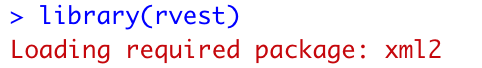
\includegraphics[width=0.6\linewidth]{/Users/carriewright/Documents/GitHub/ocs-youth-mental-health-case-study/img/rvest} \end{center}

In this case, we are scraping Table 11.1A from the website. First, we
assign the URL to a character string to use within the
\texttt{read\_html()} function in the \texttt{xml2} package.

\begin{Shaded}
\begin{Highlighting}[]
\NormalTok{NSDUH_url <-}\StringTok{ "https://www.samhsa.gov/data/sites/default/files/cbhsq-reports/NSDUHDetailedTabs2018R2/NSDUHDetTabsSect11pe2018.htm"}
\end{Highlighting}
\end{Shaded}

One could also directly use the URL but this is less convenient for
piping.

\begin{center}\rule{0.5\linewidth}{0.5pt}\end{center}

Click here if you are unfamiliar with piping in R, which uses this
\texttt{\%\textgreater{}\%} operator

By
\href{https://cran.r-project.org/web/packages/magrittr/vignettes/magrittr.html}{piping}
we mean using the \texttt{\%\textgreater{}\%} pipe operator which is
accessible after loading the \texttt{tidyverse} or several of the
packages within the tidyverse like \texttt{dplyr} because they load the
\href{https://cran.r-project.org/web/packages/magrittr/vignettes/magrittr.html}{\texttt{magrittr}
package}. This allows us to perform multiple sequential steps on one
data input.

\begin{center}\rule{0.5\linewidth}{0.5pt}\end{center}

Then, the \texttt{read\_html()} function allows us to save the html
document for the webpage inside R.

\begin{Shaded}
\begin{Highlighting}[]
\NormalTok{webpage <-}\StringTok{ }\NormalTok{NSDUH_url }\OperatorTok
\StringTok{  }\NormalTok{xml2}\OperatorTok{::}\KeywordTok{read_html}\NormalTok{() }
\NormalTok{webpage}
\end{Highlighting}
\end{Shaded}

\begin{verbatim}
{html_document}
<html lang="en">
[1] <head>\n<!-- Google Tag Manager --><script>(function(w,d,s,l,i){w[l]=w[l] ...
[2] <body>\r\n<!-- Google Tag Manager (noscript) -->\r\n<noscript><iframe src ...
\end{verbatim}

Then, we use the \texttt{html\_nodes()} function of the \texttt{rvest}
package to select just the Table 11.1A element of the webpage.

See this \href{http://flukeout.github.io/\#}{tutorial} (and the
\href{https://gist.github.com/chrisman/fcb0a88459cd98239dbe6d2d200b02d1}{answers}
in case you get stuck) on CSS selectors to understand more about how
this function works to use the \texttt{xpath} to select the elements of
interest from the webpage.

\begin{Shaded}
\begin{Highlighting}[]
\NormalTok{webpage_element <-}\StringTok{ }\NormalTok{webpage }\OperatorTok
\StringTok{  }\NormalTok{rvest}\OperatorTok{::}\KeywordTok{html_nodes}\NormalTok{(}\DataTypeTok{xpath=}\StringTok{'/html/body/div[4]/div[1]/table'}\NormalTok{)}
\NormalTok{webpage_element }
\end{Highlighting}
\end{Shaded}

\begin{verbatim}
{xml_nodeset (1)}
[1] <table class="rti">\n<caption>Table 11.1A – Settings Where Mental Health  ...
\end{verbatim}

Finally, the \texttt{html\_table()} function of the \texttt{rvest}
package parses the html object into a data frame. We can use the
\texttt{glimpse()} function of the \texttt{dplyr} package to take a look
at the data. This function shows data frames sideways with the columns
listed on the far left.

\begin{Shaded}
\begin{Highlighting}[]
\NormalTok{table11}\FloatTok{.1}\NormalTok{a <-}\StringTok{ }\NormalTok{webpage_element }\OperatorTok
\StringTok{  }\NormalTok{rvest}\OperatorTok{::}\KeywordTok{html_table}\NormalTok{()}

\KeywordTok{print}\NormalTok{(table11}\FloatTok{.1}\NormalTok{a, }\DataTypeTok{max =} \DecValTok{2}\NormalTok{)}
\end{Highlighting}
\end{Shaded}

\begin{verbatim}
[[1]]
     Setting Where Mental Health ServiceWas Received 2002 2003 2004 2005 2006
     2007 2008 2009 2010 2011 2012 2013 2014 2015 2016 2017 2018
 [ reached 'max' / getOption("max.print") -- omitted 21 rows ]
\end{verbatim}

\begin{Shaded}
\begin{Highlighting}[]
\KeywordTok{glimpse}\NormalTok{(table11}\FloatTok{.1}\NormalTok{a)}
\end{Highlighting}
\end{Shaded}

\begin{verbatim}
List of 1
 $ :'data.frame':   21 obs. of  18 variables:
  ..$ Setting Where Mental Health ServiceWas Received: chr [1:21] "SPECIALTY MENTAL HEALTH SERVICE1" "Outpatient" "Private Therapist, Psychologist,\r\n   Psychiatrist, Social Worker, or\r\n   Counselor" "Mental Health Clinic or Center" ...
  ..$ 2002                                           : chr [1:21] "2,898a" "2,662a" "2,254a" "611a" ...
  ..$ 2003                                           : chr [1:21] "3,065a" "2,795a" "2,347a" "635a" ...
  ..$ 2004                                           : chr [1:21] "3,348a" "3,015a" "2,523a" "716a" ...
  ..$ 2005                                           : chr [1:21] "3,362a" "3,048a" "2,573a" "657a" ...
  ..$ 2006                                           : chr [1:21] "3,255a" "2,931a" "2,416a" "587a" ...
  ..$ 2007                                           : chr [1:21] "3,104a" "2,787a" "2,365a" "583a" ...
  ..$ 2008                                           : chr [1:21] "3,129a" "2,837a" "2,408a" "567a" ...
  ..$ 2009                                           : chr [1:21] "2,925a" "2,650a" "2,296a" "537a" ...
  ..$ 2010                                           : chr [1:21] "2,920a" "2,635a" "2,265a" "547a" ...
  ..$ 2011                                           : chr [1:21] "3,101a" "2,842a" "2,409a" "547a" ...
  ..$ 2012                                           : chr [1:21] "3,118a" "2,846a" "2,427a" "610a" ...
  ..$ 2013                                           : chr [1:21] "3,341a" "3,064a" "2,572a" "731a" ...
  ..$ 2014                                           : chr [1:21] "3,369a" "3,110a" "2,698a" "760a" ...
  ..$ 2015                                           : chr [1:21] "3,253a" "2,958a" "2,532a" "792a" ...
  ..$ 2016                                           : chr [1:21] "3,598a" "3,239a" "2,819a" "929" ...
  ..$ 2017                                           : chr [1:21] "3,646a" "3,328" "2,908" "995" ...
  ..$ 2018                                           : chr [1:21] "3,901" "3,547" "3,080" "977" ...
\end{verbatim}

We can see that the output is a list with one element, to extract the
data from the list we will use brackets \texttt{{[}{[}{]}{]}} to select
the first element of the list.

\begin{Shaded}
\begin{Highlighting}[]
\NormalTok{table11}\FloatTok{.1}\NormalTok{a <-}\StringTok{ }\NormalTok{table11}\FloatTok{.1}\NormalTok{a[[}\DecValTok{1}\NormalTok{]]}
\end{Highlighting}
\end{Shaded}

Putting this all of this together we can do the entire process like this
with our pipe operator \texttt{\%\textgreater{}\%}.

\begin{Shaded}
\begin{Highlighting}[]
\NormalTok{table11}\FloatTok{.1}\NormalTok{a <-}\StringTok{ }\NormalTok{NSDUH_url }\OperatorTok
\StringTok{  }\NormalTok{xml2}\OperatorTok{::}\KeywordTok{read_html}\NormalTok{() }\OperatorTok
\StringTok{  }\NormalTok{rvest}\OperatorTok{::}\KeywordTok{html_nodes}\NormalTok{(}\DataTypeTok{xpath =} \StringTok{'/html/body/div[4]/div[1]/table'}\NormalTok{) }\OperatorTok
\StringTok{  }\NormalTok{rvest}\OperatorTok{::}\KeywordTok{html_table}\NormalTok{()}
\NormalTok{table11}\FloatTok{.1}\NormalTok{a <-}\StringTok{ }\NormalTok{table11}\FloatTok{.1}\NormalTok{a[[}\DecValTok{1}\NormalTok{]]}
\end{Highlighting}
\end{Shaded}

Now, we need to repeat the above process for the other tables we are
interested in.

\hypertarget{writing-a-function-to-scrape-multiple-tables}{%
\subsubsection{\texorpdfstring{\textbf{Writing a function to scrape
multiple
tables}}{Writing a function to scrape multiple tables}}\label{writing-a-function-to-scrape-multiple-tables}}

\begin{center}\rule{0.5\linewidth}{0.5pt}\end{center}

One option is to copy and paste code we wrote above. However, this is
not very efficient and is error prone. Alternatively, we can create an R
function to accomplish this succinctly. Functions allow us to perform
the same process on multiple data inputs. See
\href{https://opencasestudies.github.io/ocs-bloomberg-vaping-case-study/}{this
other case study} for more details about how to write a function.

In general, the process of writing functions involves first specifying
an input that is used within the function to create an output. In this
case, \texttt{XPATH} will be used as an ``input argument'' to the
function, which will be replaced by an actual XPath and then used in the
subsequent steps to scrape the data from each table that an XPath is
supplied for.

We will call this function \texttt{scraper}.

\begin{Shaded}
\begin{Highlighting}[]
\NormalTok{scraper <-}\StringTok{ }\ControlFlowTok{function}\NormalTok{(XPATH)\{}
\NormalTok{  NSDUH_url <-}\StringTok{ "https://www.samhsa.gov/data/sites/default/files/cbhsq-reports/NSDUHDetailedTabs2018R2/NSDUHDetTabsSect11pe2018.htm"}
\NormalTok{  table <-}\StringTok{ }\NormalTok{NSDUH_url }\OperatorTok
\StringTok{    }\KeywordTok{read_html}\NormalTok{() }\OperatorTok
\StringTok{    }\KeywordTok{html_nodes}\NormalTok{(}\DataTypeTok{xpath =}\NormalTok{ XPATH) }\OperatorTok
\StringTok{    }\KeywordTok{html_table}\NormalTok{()}
\NormalTok{  output <-}\StringTok{ }\NormalTok{table[[}\DecValTok{1}\NormalTok{]]}
\NormalTok{  output}
\NormalTok{\}}
\end{Highlighting}
\end{Shaded}

Now we can apply the function we created to each of the XPaths for each
of the tables on the website that we would like to use in our data
analysis.

\begin{Shaded}
\begin{Highlighting}[]
\NormalTok{table11}\FloatTok{.1}\NormalTok{b <-}\StringTok{ }\KeywordTok{scraper}\NormalTok{(}\DataTypeTok{XPATH =} \StringTok{"/html/body/div[4]/div[2]/table"}\NormalTok{)}
\NormalTok{table11}\FloatTok{.2}\NormalTok{a <-}\StringTok{ }\KeywordTok{scraper}\NormalTok{(}\DataTypeTok{XPATH =} \StringTok{'/html/body/div[4]/div[3]/table'}\NormalTok{)}
\NormalTok{table11}\FloatTok{.2}\NormalTok{b <-}\StringTok{ }\KeywordTok{scraper}\NormalTok{(}\DataTypeTok{XPATH =} \StringTok{'/html/body/div[4]/div[4]/table'}\NormalTok{)}
\NormalTok{table11}\FloatTok{.3}\NormalTok{a <-}\StringTok{ }\KeywordTok{scraper}\NormalTok{(}\DataTypeTok{XPATH =} \StringTok{'/html/body/div[4]/div[5]/table'}\NormalTok{)}
\NormalTok{table11}\FloatTok{.3}\NormalTok{b <-}\StringTok{ }\KeywordTok{scraper}\NormalTok{(}\DataTypeTok{XPATH =} \StringTok{'/html/body/div[4]/div[6]/table'}\NormalTok{)}
\NormalTok{table11}\FloatTok{.4}\NormalTok{a <-}\StringTok{ }\KeywordTok{scraper}\NormalTok{(}\DataTypeTok{XPATH =} \StringTok{'/html/body/div[4]/div[7]/table'}\NormalTok{)}
\NormalTok{table11}\FloatTok{.4}\NormalTok{b <-}\StringTok{ }\KeywordTok{scraper}\NormalTok{(}\DataTypeTok{XPATH =} \StringTok{'/html/body/div[4]/div[8]/table'}\NormalTok{)}
\end{Highlighting}
\end{Shaded}

Great! We have successfully scraped the data from the web into R!

Next, we need to wrangle the data.

We will save the data now in case the website gets removed in the
future. To do this we will use the base \texttt{save()} function.

\begin{Shaded}
\begin{Highlighting}[]
\KeywordTok{save}\NormalTok{(table11}\FloatTok{.1}\NormalTok{a, table11}\FloatTok{.1}\NormalTok{b, table11}\FloatTok{.2}\NormalTok{a, table11}\FloatTok{.2}\NormalTok{b, }
\NormalTok{     table11}\FloatTok{.3}\NormalTok{a, table11}\FloatTok{.3}\NormalTok{b, table11}\FloatTok{.4}\NormalTok{a, table11}\FloatTok{.4}\NormalTok{b, }\DataTypeTok{file =}\NormalTok{ here}\OperatorTok{::}\KeywordTok{here}\NormalTok{(}\StringTok{"data"}\NormalTok{, }\StringTok{"raw_data.rda"}\NormalTok{))}
\end{Highlighting}
\end{Shaded}

\hypertarget{data-wrangling}{%
\subsection{\texorpdfstring{\textbf{Data
Wrangling}}{Data Wrangling}}\label{data-wrangling}}

\begin{center}\rule{0.5\linewidth}{0.5pt}\end{center}

Now that we have imported the data, let's see if we can wrangle a table.

What do we mean by ``wrangle''? We mean that we intend to get the data
into what is called ``tidy'' format.

This means that the data:\\
1) has each observation in single row\\
2) has a single aspect about each observation as a single column\\
3) is rectangular (meaning there are no empty cells)\\
4) the values within the cells are in a format that is useful for making
visualizations and for analysis

Check out this \href{https://vita.had.co.nz/papers/tidy-data.pdf}{paper}
for more information about tidy data.

Since the data appear to be formatted in a similar way in each of the
tables, it is likely that whatever steps we take to wrangle this first
table will also be necessary in the wrangling of subsequent tables. This
is because well-maintained data sources often format different datasets
similarly. We can take advantage of this similarity to speed up the
wrangling process.

\hypertarget{table11.1a}{%
\subsubsection{\texorpdfstring{\textbf{Table11.1a}}{Table11.1a}}\label{table11.1a}}

\begin{center}\rule{0.5\linewidth}{0.5pt}\end{center}

Let's take a look at our table on the website to see what it needs to
get it into ``tidy'' format.

First, we can see that we want to remove the legend of our table.

\begin{center}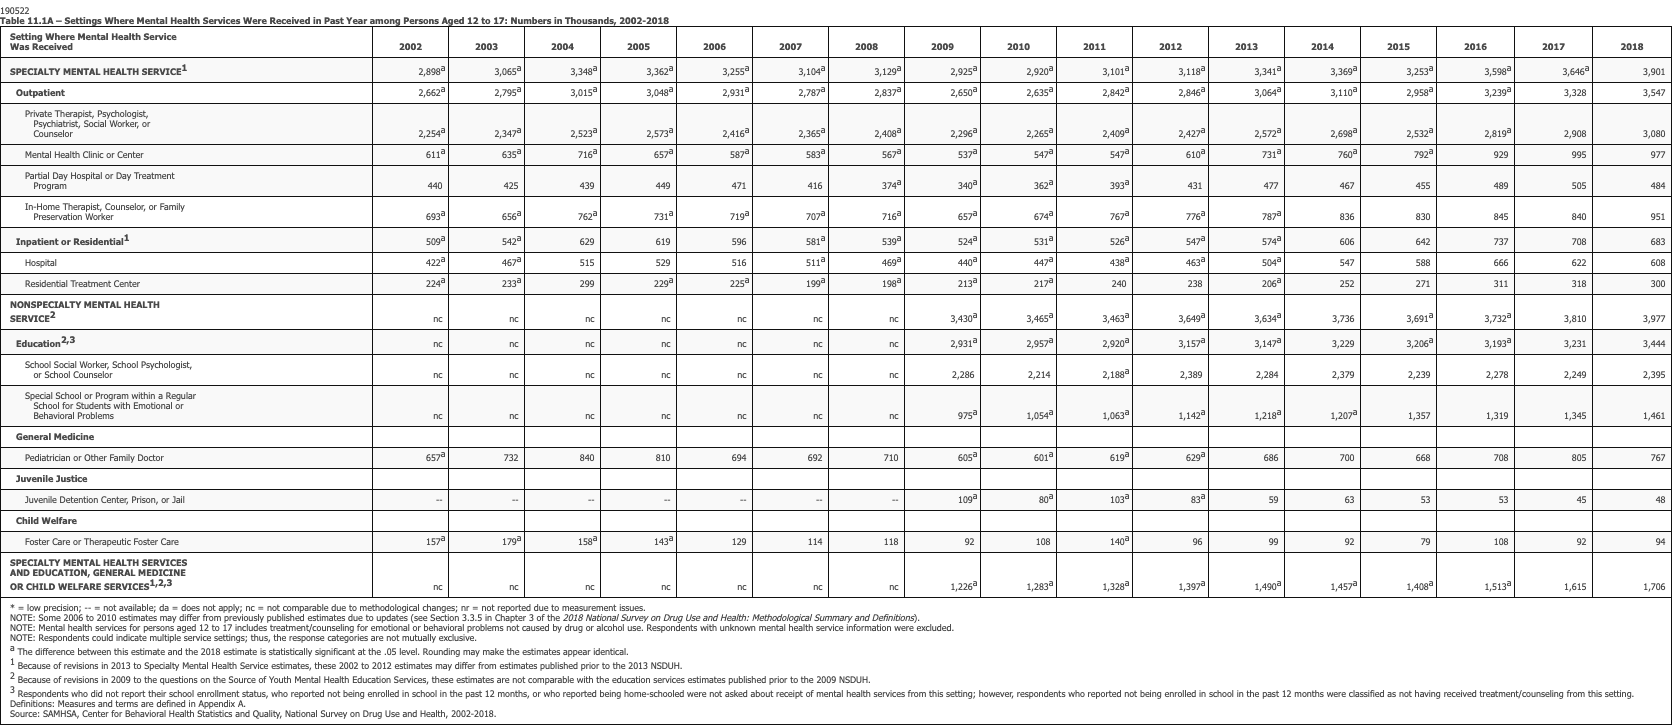
\includegraphics[width=0.9\linewidth]{/Users/carriewright/Documents/GitHub/ocs-youth-mental-health-case-study/img/table11.1a} \end{center}

We can take a look at the last row using the \texttt{tail} function of
the \texttt{dplyr} package. We can specify that we only want to see the
last row by using the \texttt{n\ =\ 1} argument. To use the
\texttt{dplyr} functions we need to first make this table into a tibble,
which is the \texttt{tidyverse} version of a dataframe.

Currently table11.1a is a typical dataframe, which we can see using the
\texttt{class} function which describes the types of data objects in R.

\begin{Shaded}
\begin{Highlighting}[]
\KeywordTok{class}\NormalTok{(table11}\FloatTok{.1}\NormalTok{a)}
\end{Highlighting}
\end{Shaded}

\begin{verbatim}
[1] "data.frame"
\end{verbatim}

We can use the \texttt{as\_tibble()} function of the \texttt{dplyr}
package to convert \texttt{table11.1a} into a tibble.

\begin{Shaded}
\begin{Highlighting}[]
\NormalTok{table11}\FloatTok{.1}\NormalTok{a }\OperatorTok
\StringTok{  }\NormalTok{dplyr}\OperatorTok{::}\KeywordTok{as_tibble}\NormalTok{() }\OperatorTok
\StringTok{  }\KeywordTok{tail}\NormalTok{(}\DataTypeTok{n =} \DecValTok{1}\NormalTok{)}
\end{Highlighting}
\end{Shaded}

\begin{verbatim}
# A tibble: 1 x 18
  `Setting Where ~ `2002` `2003` `2004` `2005` `2006` `2007` `2008` `2009`
  <chr>            <chr>  <chr>  <chr>  <chr>  <chr>  <chr>  <chr>  <chr> 
1 "* = low precis~ "* = ~ "* = ~ "* = ~ "* = ~ "* = ~ "* = ~ "* = ~ "* = ~
# ... with 9 more variables: `2010` <chr>, `2011` <chr>, `2012` <chr>,
#   `2013` <chr>, `2014` <chr>, `2015` <chr>, `2016` <chr>, `2017` <chr>,
#   `2018` <chr>
\end{verbatim}

We can see that the legend is repeated for every column. Now, let's take
a look at the year 2004 column.

\begin{Shaded}
\begin{Highlighting}[]
\NormalTok{table11}\FloatTok{.1}\NormalTok{a }\OperatorTok
\StringTok{  }\NormalTok{dplyr}\OperatorTok{::}\KeywordTok{as_tibble}\NormalTok{() }\OperatorTok\StringTok{  }
\StringTok{  }\NormalTok{dplyr}\OperatorTok{::}\KeywordTok{select}\NormalTok{(}\StringTok{`}\DataTypeTok{2004}\StringTok{`}\NormalTok{) }\OperatorTok
\StringTok{  }\KeywordTok{tail}\NormalTok{(}\DataTypeTok{n =} \DecValTok{1}\NormalTok{)}
\end{Highlighting}
\end{Shaded}

\begin{verbatim}
# A tibble: 1 x 1
  `2004`                                                                        
  <chr>                                                                         
1 "* = low precision; -- = not available; da = does not apply; nc = not compara~
\end{verbatim}

Let's save this to an object called \texttt{legend} so that we can refer
back to it later:

\begin{Shaded}
\begin{Highlighting}[]
\NormalTok{legend <-}\StringTok{ }\NormalTok{table11}\FloatTok{.1}\NormalTok{a }\OperatorTok
\StringTok{  }\KeywordTok{as_tibble}\NormalTok{() }\OperatorTok\StringTok{  }
\StringTok{  }\KeywordTok{select}\NormalTok{(}\StringTok{`}\DataTypeTok{2004}\StringTok{`}\NormalTok{) }\OperatorTok
\StringTok{  }\KeywordTok{tail}\NormalTok{(}\DataTypeTok{n =} \DecValTok{1}\NormalTok{)}
\end{Highlighting}
\end{Shaded}

Another way to look at the last row is to use the \texttt{n()} function
of the \texttt{dplyr} package. This function can be used inside other
\texttt{dplyr} functions and it counts the total number of observations
of a group. Within the
\href{https://dplyr.tidyverse.org/reference/slice.html}{\texttt{slice()}
function} of the \texttt{dplyr} package, it allows you to refer the full
length of the object.

\begin{Shaded}
\begin{Highlighting}[]
\NormalTok{table11}\FloatTok{.1}\NormalTok{a }\OperatorTok
\StringTok{  }\NormalTok{dplyr}\OperatorTok{::}\KeywordTok{as_tibble}\NormalTok{() }\OperatorTok
\StringTok{  }\NormalTok{dplyr}\OperatorTok{::}\KeywordTok{slice}\NormalTok{(}\KeywordTok{n}\NormalTok{()) }
\end{Highlighting}
\end{Shaded}

\begin{verbatim}
# A tibble: 1 x 18
  `Setting Where ~ `2002` `2003` `2004` `2005` `2006` `2007` `2008` `2009`
  <chr>            <chr>  <chr>  <chr>  <chr>  <chr>  <chr>  <chr>  <chr> 
1 "* = low precis~ "* = ~ "* = ~ "* = ~ "* = ~ "* = ~ "* = ~ "* = ~ "* = ~
# ... with 9 more variables: `2010` <chr>, `2011` <chr>, `2012` <chr>,
#   `2013` <chr>, `2014` <chr>, `2015` <chr>, `2016` <chr>, `2017` <chr>,
#   `2018` <chr>
\end{verbatim}

We can use the \texttt{slice()} function of the \texttt{dplyr} package
to remove this row, by using the \texttt{slice}function to select from
the first row using \texttt{1:} to the second to last row using
\texttt{n()-1}.

We are also going to use a special pipe operator from the
\href{https://cran.r-project.org/web/packages/magrittr/vignettes/magrittr.html}{\texttt{magrittr}
package} called the compound assignment pipe-operator or sometimes the
double pipe operator. This allows us to use the \texttt{table11.1a} as
our input and reassign it at the end after all the steps have been
performed.

We will also first change the data to be a
\href{https://tibble.tidyverse.org/\#:~:text=A\%20tibble\%2C\%20or\%20tbl_df\%20\%2C\%20is,modern\%20reimagining\%20of\%20the\%20data.\&text=Tibbles\%20are\%20data.,a\%20variable\%20does\%20not\%20exist}{tibble}.),
which is the \texttt{tidyverse} version of a data frame using the
\texttt{as\_tibble()} function of the \texttt{dplyr} package and the
\texttt{tibble} package.

\begin{Shaded}
\begin{Highlighting}[]
\NormalTok{table11}\FloatTok{.1}\NormalTok{a }\OperatorTok
\StringTok{  }\NormalTok{dplyr}\OperatorTok{::}\KeywordTok{as_tibble}\NormalTok{() }\OperatorTok
\StringTok{  }\KeywordTok{slice}\NormalTok{(}\DecValTok{1}\OperatorTok{:}\NormalTok{(}\KeywordTok{n}\NormalTok{()}\OperatorTok{-}\DecValTok{1}\NormalTok{))}
\end{Highlighting}
\end{Shaded}

Now let's take a look at the data:

\begin{Shaded}
\begin{Highlighting}[]
\KeywordTok{slice_head}\NormalTok{(table11}\FloatTok{.1}\NormalTok{a, }\DataTypeTok{n =}\NormalTok{ (}\KeywordTok{length}\NormalTok{(}\KeywordTok{pull}\NormalTok{(table11}\FloatTok{.1}\NormalTok{a, }\StringTok{`}\DataTypeTok{2002}\StringTok{`}\NormalTok{))))}
\end{Highlighting}
\end{Shaded}

\begin{verbatim}
# A tibble: 20 x 18
   `Setting Where ~ `2002` `2003` `2004` `2005` `2006` `2007` `2008` `2009`
   <chr>            <chr>  <chr>  <chr>  <chr>  <chr>  <chr>  <chr>  <chr> 
 1 "SPECIALTY MENT~ "2,89~ "3,06~ "3,34~ "3,36~ "3,25~ "3,10~ "3,12~ "2,92~
 2 "Outpatient"     "2,66~ "2,79~ "3,01~ "3,04~ "2,93~ "2,78~ "2,83~ "2,65~
 3 "Private Therap~ "2,25~ "2,34~ "2,52~ "2,57~ "2,41~ "2,36~ "2,40~ "2,29~
 4 "Mental Health ~ "611a" "635a" "716a" "657a" "587a" "583a" "567a" "537a"
 5 "Partial Day Ho~ "440"  "425"  "439"  "449"  "471"  "416"  "374a" "340a"
 6 "In-Home Therap~ "693a" "656a" "762a" "731a" "719a" "707a" "716a" "657a"
 7 "Inpatient or R~ "509a" "542a" "629"  "619"  "596"  "581a" "539a" "524a"
 8 "Hospital"       "422a" "467a" "515"  "529"  "516"  "511a" "469a" "440a"
 9 "Residential Tr~ "224a" "233a" "299"  "229a" "225a" "199a" "198a" "213a"
10 "NONSPECIALTY M~ "nc"   "nc"   "nc"   "nc"   "nc"   "nc"   "nc"   "3,43~
11 "Education2,3"   "nc"   "nc"   "nc"   "nc"   "nc"   "nc"   "nc"   "2,93~
12 "School Social ~ "nc"   "nc"   "nc"   "nc"   "nc"   "nc"   "nc"   "2,28~
13 "Special School~ "nc"   "nc"   "nc"   "nc"   "nc"   "nc"   "nc"   "975a"
14 "General Medici~ ""     ""     ""     ""     ""     ""     ""     ""    
15 "Pediatrician o~ "657a" "732"  "840"  "810"  "694"  "692"  "710"  "605a"
16 "Juvenile Justi~ ""     ""     ""     ""     ""     ""     ""     ""    
17 "Juvenile Deten~ "--"   "--"   "--"   "--"   "--"   "--"   "--"   "109a"
18 "Child Welfare"  ""     ""     ""     ""     ""     ""     ""     ""    
19 "Foster Care or~ "157a" "179a" "158a" "143a" "129"  "114"  "118"  "92"  
20 "SPECIALTY MENT~ "nc"   "nc"   "nc"   "nc"   "nc"   "nc"   "nc"   "1,22~
# ... with 9 more variables: `2010` <chr>, `2011` <chr>, `2012` <chr>,
#   `2013` <chr>, `2014` <chr>, `2015` <chr>, `2016` <chr>, `2017` <chr>,
#   `2018` <chr>
\end{verbatim}

Great! We can see the the legend is no longer part of the data.

Now let's use the legend to recode the data. There are many different
values for missing data, that we would like to replace with \texttt{NA}
instead. We can use the \texttt{pull()} function of the \texttt{dplyr}
package to take a look at the legend data:

\begin{Shaded}
\begin{Highlighting}[]
\NormalTok{dplyr}\OperatorTok{::}\KeywordTok{pull}\NormalTok{(legend, }\StringTok{`}\DataTypeTok{2004}\StringTok{`}\NormalTok{)}
\end{Highlighting}
\end{Shaded}

\begin{verbatim}
[1] "* = low precision; -- = not available; da = does not apply; nc = not comparable due to methodological changes; nr = not reported due to measurement issues.\r\nNOTE: Some 2006 to 2010 estimates may differ from previously published estimates due to updates (see Section 3.3.5 in Chapter 3 of the 2018 National Survey on Drug Use and Health: Methodological Summary and Definitions).\r\nNOTE: Mental health services for persons aged 12 to 17 includes treatment/counseling for emotional or behavioral problems not caused by drug or alcohol use. Respondents with unknown mental health service information were excluded.\r\nNOTE: Respondents could indicate multiple service settings; thus, the response categories are not mutually exclusive.a The difference between this estimate and the 2018 estimate is statistically significant at the .05 level. Rounding may make the estimates appear identical.1 Because of revisions in 2013 to Specialty Mental Health Service estimates, these 2002 to 2012 estimates may differ from estimates published prior to the 2013 NSDUH.2 Because of revisions in 2009 to the questions on the Source of Youth Mental Health Education Services, these estimates are not comparable with the education services estimates published prior to the 2009 NSDUH.3 Respondents who did not report their school enrollment status, who reported not being enrolled in school in the past 12 months, or who reported being home-schooled were not asked about receipt of mental health services from this setting; however, respondents who reported not being enrolled in school in the past 12 months were classified as not having received treatment/counseling from this setting.\r\nDefinitions: Measures and terms are defined in Appendix A.\r\nSource: SAMHSA, Center for Behavioral Health Statistics and Quality, National Survey on Drug Use and Health, 2002-2018."
\end{verbatim}

Looks like we want to replace values that are: \texttt{*},
\texttt{-\/-}, \texttt{da}, \texttt{nc}, and \texttt{nr}.

We can use the \texttt{na\_if()} function to recode these values to
\texttt{NA}.

\begin{Shaded}
\begin{Highlighting}[]
\NormalTok{table11}\FloatTok{.1}\NormalTok{a }\OperatorTok
\StringTok{  }\NormalTok{dplyr}\OperatorTok{::}\KeywordTok{na_if}\NormalTok{(}\StringTok{"nc"}\NormalTok{) }\OperatorTok
\StringTok{  }\NormalTok{dplyr}\OperatorTok{::}\KeywordTok{na_if}\NormalTok{(}\StringTok{"--"}\NormalTok{) }\OperatorTok
\StringTok{  }\NormalTok{dplyr}\OperatorTok{::}\KeywordTok{na_if}\NormalTok{(}\StringTok{""}\NormalTok{) }\OperatorTok
\StringTok{  }\NormalTok{dplyr}\OperatorTok{::}\KeywordTok{na_if}\NormalTok{(}\StringTok{"*"}\NormalTok{)}

\KeywordTok{head}\NormalTok{(table11}\FloatTok{.1}\NormalTok{a)}
\end{Highlighting}
\end{Shaded}

\begin{verbatim}
# A tibble: 6 x 18
  `Setting Where ~ `2002` `2003` `2004` `2005` `2006` `2007` `2008` `2009`
  <chr>            <chr>  <chr>  <chr>  <chr>  <chr>  <chr>  <chr>  <chr> 
1 "SPECIALTY MENT~ 2,898a 3,065a 3,348a 3,362a 3,255a 3,104a 3,129a 2,925a
2 "Outpatient"     2,662a 2,795a 3,015a 3,048a 2,931a 2,787a 2,837a 2,650a
3 "Private Therap~ 2,254a 2,347a 2,523a 2,573a 2,416a 2,365a 2,408a 2,296a
4 "Mental Health ~ 611a   635a   716a   657a   587a   583a   567a   537a  
5 "Partial Day Ho~ 440    425    439    449    471    416    374a   340a  
6 "In-Home Therap~ 693a   656a   762a   731a   719a   707a   716a   657a  
# ... with 9 more variables: `2010` <chr>, `2011` <chr>, `2012` <chr>,
#   `2013` <chr>, `2014` <chr>, `2015` <chr>, `2016` <chr>, `2017` <chr>,
#   `2018` <chr>
\end{verbatim}

Let's look at the column names in our table:

\begin{Shaded}
\begin{Highlighting}[]
\KeywordTok{colnames}\NormalTok{(table11}\FloatTok{.1}\NormalTok{a)}
\end{Highlighting}
\end{Shaded}

\begin{verbatim}
 [1] "Setting Where Mental Health ServiceWas Received"
 [2] "2002"                                           
 [3] "2003"                                           
 [4] "2004"                                           
 [5] "2005"                                           
 [6] "2006"                                           
 [7] "2007"                                           
 [8] "2008"                                           
 [9] "2009"                                           
[10] "2010"                                           
[11] "2011"                                           
[12] "2012"                                           
[13] "2013"                                           
[14] "2014"                                           
[15] "2015"                                           
[16] "2016"                                           
[17] "2017"                                           
[18] "2018"                                           
\end{verbatim}

Let's rename the first column using the \texttt{rename()} function of
the \texttt{dplyr} package. This requires listing the new name first
like so: \texttt{new\_name\ =\ old\_name}.

\begin{Shaded}
\begin{Highlighting}[]
\NormalTok{table11}\FloatTok{.1}\NormalTok{a }\OperatorTok
\StringTok{  }\NormalTok{dplyr}\OperatorTok{::}\KeywordTok{rename}\NormalTok{(}\DataTypeTok{MHS_setting =} \StringTok{`}\DataTypeTok{Setting Where Mental Health ServiceWas Received}\StringTok{`}\NormalTok{)}

\KeywordTok{head}\NormalTok{(table11}\FloatTok{.1}\NormalTok{a)}
\end{Highlighting}
\end{Shaded}

\begin{verbatim}
# A tibble: 6 x 18
  MHS_setting `2002` `2003` `2004` `2005` `2006` `2007` `2008` `2009` `2010`
  <chr>       <chr>  <chr>  <chr>  <chr>  <chr>  <chr>  <chr>  <chr>  <chr> 
1 "SPECIALTY~ 2,898a 3,065a 3,348a 3,362a 3,255a 3,104a 3,129a 2,925a 2,920a
2 "Outpatien~ 2,662a 2,795a 3,015a 3,048a 2,931a 2,787a 2,837a 2,650a 2,635a
3 "Private T~ 2,254a 2,347a 2,523a 2,573a 2,416a 2,365a 2,408a 2,296a 2,265a
4 "Mental He~ 611a   635a   716a   657a   587a   583a   567a   537a   547a  
5 "Partial D~ 440    425    439    449    471    416    374a   340a   362a  
6 "In-Home T~ 693a   656a   762a   731a   719a   707a   716a   657a   674a  
# ... with 8 more variables: `2011` <chr>, `2012` <chr>, `2013` <chr>,
#   `2014` <chr>, `2015` <chr>, `2016` <chr>, `2017` <chr>, `2018` <chr>
\end{verbatim}

Nice!

Now you may notice that the individual values for the year columns have
an \texttt{"a"} after the numeric value.

According to the legend this indicates if ``the difference between this
estimate and the 2018 estimate is significant at the \(\alpha\)=.05
level.''

While this is useful information, it makes it difficult to work with our
numeric values, so we want to remove them.

Since lower case \texttt{"a"} values occur in the values of the
\texttt{MHS\_setting} column (like outp\textbf{a}tient), we want to make
sure that we don't just remove all \texttt{"a"} values from the table,
just those in the subsequent columns.

So how can we do this? We can use the \texttt{stringr} package to modify
character strings. Also, we can use the \texttt{dplyr} functions
\texttt{mutate()}, \texttt{select()} and \texttt{across()} to specify
want columns we want to change.

Currently all of our data are character strings as indicated by the
\texttt{\textless{}chr\textgreater{}} under the column names.

\begin{center}\rule{0.5\linewidth}{0.5pt}\end{center}

Click here for an explanation about data classes in R and about
character strings.

There are several
\href{https://en.wikipedia.org/wiki/R_(programming_language)}{classes of
data in R programming}, meaning that certain objects will be treated or
interpreted differently. Character is one of these classes. A character
string is an individual data value made up of characters. This can be a
paragraph, like the legend for the table, or it can be a single letter
or number like the letter \texttt{"a"} or the number \texttt{"3"}. If
data are of class character, than the numeric values will not be
processed like a numeric value in a mathematical sense. If you want your
numeric values to be interpreted that way, they need to be converted to
a numeric class. The options typically used are integer (which has no
decimal place) and double precision (which has a decimal place).

\begin{center}\rule{0.5\linewidth}{0.5pt}\end{center}

The \texttt{stringr} package has functions that allow us to replace
(using the \texttt{str\_replace()} function) or remove (using the
\texttt{str\_remove()} function) characters.

To use these, we need to be able to specify what we want to remove and
replace.

Here is a part of a
\href{https://rstudio.com/resources/cheatsheets/}{cheatsheet} about
string manipulation from RStudio.

\begin{center}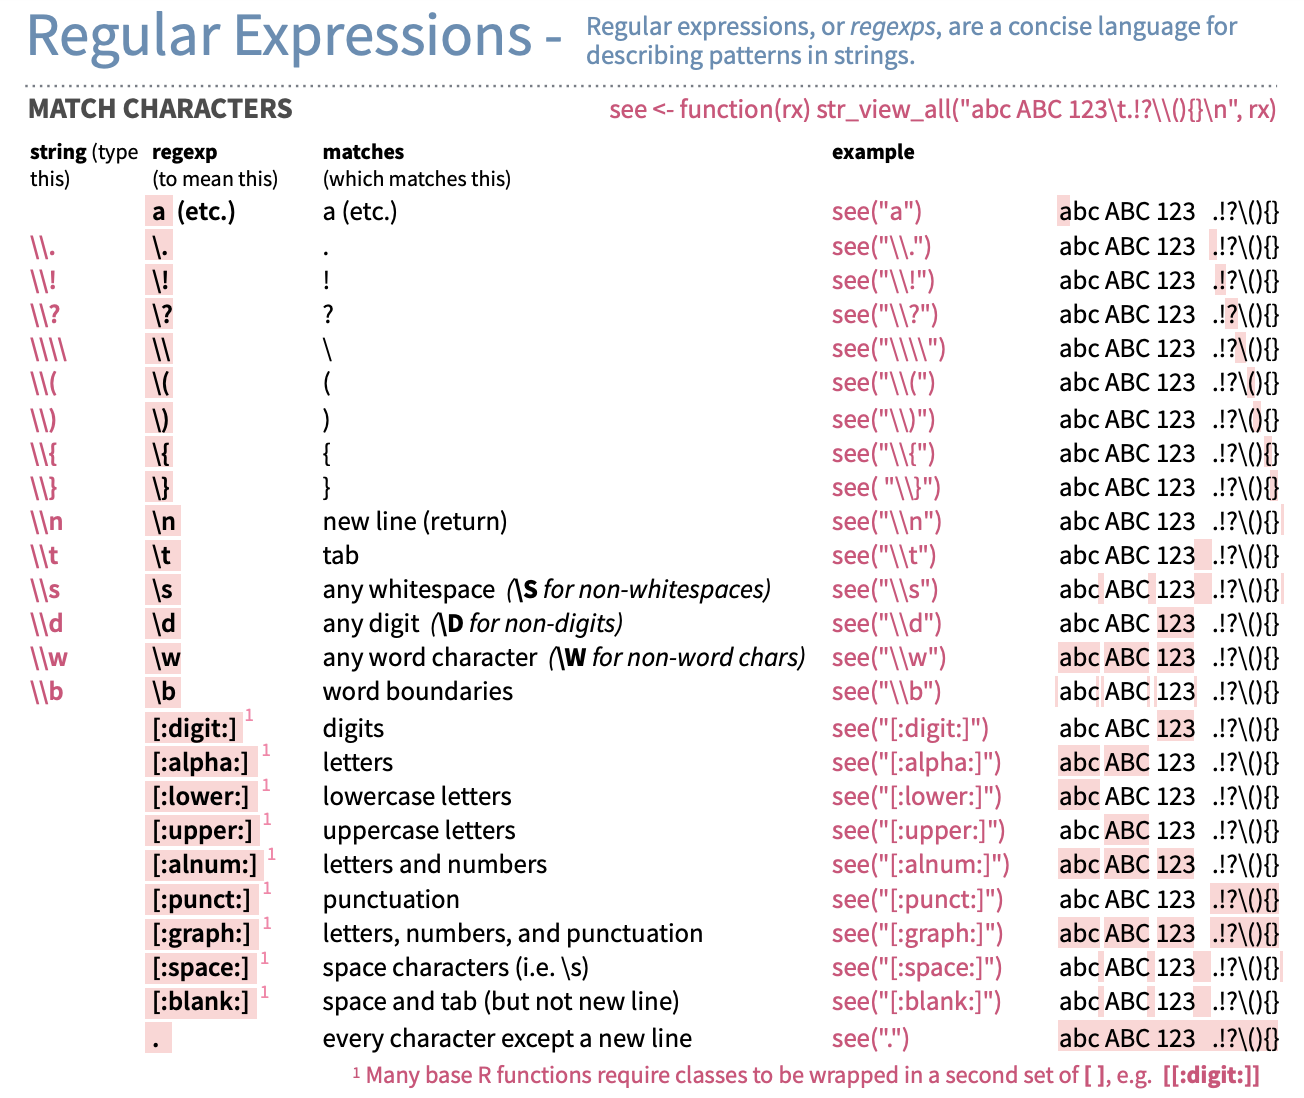
\includegraphics[width=0.9\linewidth]{/Users/carriewright/Documents/GitHub/ocs-youth-mental-health-case-study/img/regex} \end{center}

We can see that we can refer to any digit (such as 1, 2, 3 etc.) as
\texttt{{[}:digit:{]}}. We can also see that we can refer to any
punctuation mark as \texttt{{[}:punct:{]}}. Finally, we see that spaces
and tabs can be referred to as \texttt{{[}:blank:{]}}.

If we take a closer look at just the first column of our table (using
the \texttt{pull()} function of the \texttt{dplyr} package), we see that
there are also some large white spaces, some numeric values, instances
of \texttt{"\textbackslash{}r\textbackslash{}n"}, as well as some commas
and other punctuation marks that we would like to remove form this
column.

\begin{Shaded}
\begin{Highlighting}[]
\NormalTok{table11}\FloatTok{.1}\NormalTok{a }\OperatorTok\StringTok{ }
\StringTok{  }\KeywordTok{pull}\NormalTok{(MHS_setting)}
\end{Highlighting}
\end{Shaded}

\begin{verbatim}
 [1] "SPECIALTY MENTAL HEALTH SERVICE1"                                                                                
 [2] "Outpatient"                                                                                                      
 [3] "Private Therapist, Psychologist,\r\n   Psychiatrist, Social Worker, or\r\n   Counselor"                          
 [4] "Mental Health Clinic or Center"                                                                                  
 [5] "Partial Day Hospital or Day Treatment\r\n   Program"                                                             
 [6] "In-Home Therapist, Counselor, or Family\r\n   Preservation Worker"                                               
 [7] "Inpatient or Residential1"                                                                                       
 [8] "Hospital"                                                                                                        
 [9] "Residential Treatment Center"                                                                                    
[10] "NONSPECIALTY MENTAL HEALTH\r\nSERVICE2"                                                                          
[11] "Education2,3"                                                                                                    
[12] "School Social Worker, School Psychologist,\r\n   or School Counselor"                                            
[13] "Special School or Program within a Regular\r\n   School for Students with Emotional or\r\n   Behavioral Problems"
[14] "General Medicine"                                                                                                
[15] "Pediatrician or Other Family Doctor"                                                                             
[16] "Juvenile Justice"                                                                                                
[17] "Juvenile Detention Center, Prison, or Jail"                                                                      
[18] "Child Welfare"                                                                                                   
[19] "Foster Care or Therapeutic Foster Care"                                                                          
[20] "SPECIALTY MENTAL HEALTH SERVICES\r\nAND EDUCATION, GENERAL MEDICINE\r\nOR CHILD WELFARE SERVICES1,2,3"           
\end{verbatim}

We can use the \texttt{str\_remove\_all()} function to remove these
unwanted characters from this column specifically.

The \texttt{str\_remove\_all()} function is a variant of the
\texttt{str\_remove()} function of the \texttt{stringr} package. It
allows us to remove all occurrences of specified characters in each row
rather than just the first occurrence (which is what
\texttt{str\_remove()} does).

Using the \texttt{mutate()} function, we specify that we want to change
this particular column and replace it with a version of this column that
does not contain characters that are digits, the
\texttt{r\textbackslash{}n} string that we saw, or punctuation marks.

We need to specify that the character strings that should be used can be
found in the \texttt{MHS\_setting} column by using the
\texttt{string\ =} argument and the patterns to find and remove are
specified using the \texttt{pattern\ =} argument.

To allow us to look for all three of these patterns at the same time, we
can use the \texttt{\textbar{}} symbol between each pattern.

\begin{Shaded}
\begin{Highlighting}[]
\NormalTok{table11}\FloatTok{.1}\NormalTok{a }\OperatorTok
\KeywordTok{mutate}\NormalTok{(}\DataTypeTok{MHS_setting =} 
         \KeywordTok{str_remove_all}\NormalTok{(}\DataTypeTok{string =}\NormalTok{ MHS_setting, }
                        \DataTypeTok{pattern =} \StringTok{"[:digit:]|}\CharTok{\textbackslash{}r\textbackslash{}n}\StringTok{|[:punct:]|"}\NormalTok{))}

\KeywordTok{head}\NormalTok{(table11}\FloatTok{.1}\NormalTok{a)}
\end{Highlighting}
\end{Shaded}

\begin{verbatim}
# A tibble: 6 x 18
  MHS_setting `2002` `2003` `2004` `2005` `2006` `2007` `2008` `2009` `2010`
  <chr>       <chr>  <chr>  <chr>  <chr>  <chr>  <chr>  <chr>  <chr>  <chr> 
1 SPECIALTY ~ 2,898a 3,065a 3,348a 3,362a 3,255a 3,104a 3,129a 2,925a 2,920a
2 Outpatient  2,662a 2,795a 3,015a 3,048a 2,931a 2,787a 2,837a 2,650a 2,635a
3 Private Th~ 2,254a 2,347a 2,523a 2,573a 2,416a 2,365a 2,408a 2,296a 2,265a
4 Mental Hea~ 611a   635a   716a   657a   587a   583a   567a   537a   547a  
5 Partial Da~ 440    425    439    449    471    416    374a   340a   362a  
6 InHome The~ 693a   656a   762a   731a   719a   707a   716a   657a   674a  
# ... with 8 more variables: `2011` <chr>, `2012` <chr>, `2013` <chr>,
#   `2014` <chr>, `2015` <chr>, `2016` <chr>, `2017` <chr>, `2018` <chr>
\end{verbatim}

We also want to replace the spaces with a single space. We can see that
sometimes there appears to be more than one space. We can specify that
we want any occurrence of 1 or more to be replaced by using the
\texttt{\{1,\}} notation.

See here for an explanation of this on the cheat sheet:

\begin{center}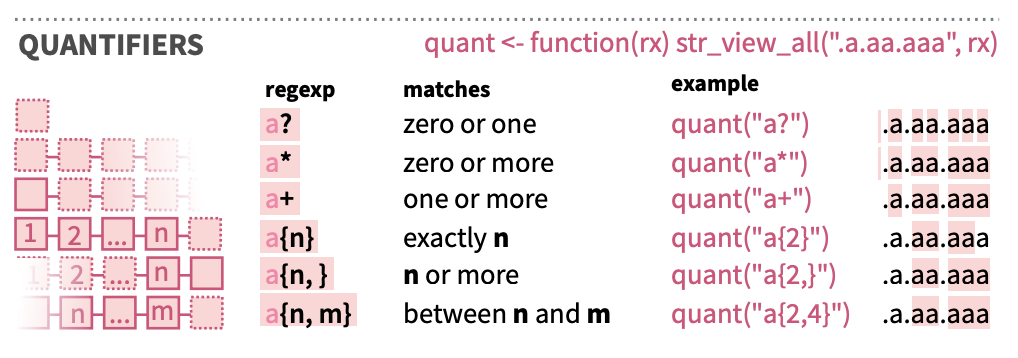
\includegraphics[width=0.9\linewidth]{/Users/carriewright/Documents/GitHub/ocs-youth-mental-health-case-study/img/quantifiers} \end{center}

So, we will use the \texttt{str\_replace\_all()} function of the
\texttt{stringr} package. In this case, we also need to specify a
replacement with the \texttt{replacement\ =} argument. We will use this
to specify one space.

\begin{Shaded}
\begin{Highlighting}[]
\NormalTok{table11}\FloatTok{.1}\NormalTok{a }\OperatorTok
\KeywordTok{mutate}\NormalTok{(}\DataTypeTok{MHS_setting =} 
         \KeywordTok{str_replace_all}\NormalTok{(}\DataTypeTok{string =}\NormalTok{ MHS_setting,}
                         \DataTypeTok{pattern =} \StringTok{"[:blank:]\{1,\}"}\NormalTok{, }
                         \DataTypeTok{replacement =} \StringTok{" "}\NormalTok{))}

\KeywordTok{head}\NormalTok{(table11}\FloatTok{.1}\NormalTok{a)}
\end{Highlighting}
\end{Shaded}

\begin{verbatim}
# A tibble: 6 x 18
  MHS_setting `2002` `2003` `2004` `2005` `2006` `2007` `2008` `2009` `2010`
  <chr>       <chr>  <chr>  <chr>  <chr>  <chr>  <chr>  <chr>  <chr>  <chr> 
1 SPECIALTY ~ 2,898a 3,065a 3,348a 3,362a 3,255a 3,104a 3,129a 2,925a 2,920a
2 Outpatient  2,662a 2,795a 3,015a 3,048a 2,931a 2,787a 2,837a 2,650a 2,635a
3 Private Th~ 2,254a 2,347a 2,523a 2,573a 2,416a 2,365a 2,408a 2,296a 2,265a
4 Mental Hea~ 611a   635a   716a   657a   587a   583a   567a   537a   547a  
5 Partial Da~ 440    425    439    449    471    416    374a   340a   362a  
6 InHome The~ 693a   656a   762a   731a   719a   707a   716a   657a   674a  
# ... with 8 more variables: `2011` <chr>, `2012` <chr>, `2013` <chr>,
#   `2014` <chr>, `2015` <chr>, `2016` <chr>, `2017` <chr>, `2018` <chr>
\end{verbatim}

Next, we will remove the \texttt{"a"} values and the commas from the
body of the table using the \texttt{str\_remove\_all()} function yet
again.

However, this time to specify that we want all columns except the first
column called \texttt{MHS\_setting}, we can use the \texttt{across()}
function of the \texttt{dplyr} package.

This allows us to specify what columns we want to mutate by using the
\texttt{.cols\ =} argument. We can select all columns except the first
column called \texttt{MHS\_setting} by using a minus sign \texttt{-} in
front of the column name.

\begin{Shaded}
\begin{Highlighting}[]
\NormalTok{table11}\FloatTok{.1}\NormalTok{a }\OperatorTok
\StringTok{  }\KeywordTok{mutate}\NormalTok{(dplyr}\OperatorTok{::}\KeywordTok{across}\NormalTok{(}\DataTypeTok{.cols =} \OperatorTok{-}\NormalTok{MHS_setting,}
\NormalTok{                       stringr}\OperatorTok{::}\NormalTok{str_remove_all, }\StringTok{"a|,"}\NormalTok{))}

\KeywordTok{head}\NormalTok{(table11}\FloatTok{.1}\NormalTok{a)}
\end{Highlighting}
\end{Shaded}

\begin{verbatim}
# A tibble: 6 x 18
  MHS_setting `2002` `2003` `2004` `2005` `2006` `2007` `2008` `2009` `2010`
  <chr>       <chr>  <chr>  <chr>  <chr>  <chr>  <chr>  <chr>  <chr>  <chr> 
1 SPECIALTY ~ 2898   3065   3348   3362   3255   3104   3129   2925   2920  
2 Outpatient  2662   2795   3015   3048   2931   2787   2837   2650   2635  
3 Private Th~ 2254   2347   2523   2573   2416   2365   2408   2296   2265  
4 Mental Hea~ 611    635    716    657    587    583    567    537    547   
5 Partial Da~ 440    425    439    449    471    416    374    340    362   
6 InHome The~ 693    656    762    731    719    707    716    657    674   
# ... with 8 more variables: `2011` <chr>, `2012` <chr>, `2013` <chr>,
#   `2014` <chr>, `2015` <chr>, `2016` <chr>, `2017` <chr>, `2018` <chr>
\end{verbatim}

Our table is looking much better!

We also want to change our values to be numeric as opposed to character
so that we can use them in mathematical functions. We can use the base
\texttt{as.numeric()} function. Again we will use the \texttt{across()}
function to indicate what variables we wish to mutate.

\begin{Shaded}
\begin{Highlighting}[]
\NormalTok{table11}\FloatTok{.1}\NormalTok{a }\OperatorTok
\StringTok{  }\KeywordTok{mutate}\NormalTok{(}\KeywordTok{across}\NormalTok{(}\DataTypeTok{.cols =}\OperatorTok{-}\NormalTok{MHS_setting, as.numeric))}

\KeywordTok{head}\NormalTok{(table11}\FloatTok{.1}\NormalTok{a)}
\end{Highlighting}
\end{Shaded}

\begin{verbatim}
# A tibble: 6 x 18
  MHS_setting `2002` `2003` `2004` `2005` `2006` `2007` `2008` `2009` `2010`
  <chr>        <dbl>  <dbl>  <dbl>  <dbl>  <dbl>  <dbl>  <dbl>  <dbl>  <dbl>
1 SPECIALTY ~   2898   3065   3348   3362   3255   3104   3129   2925   2920
2 Outpatient    2662   2795   3015   3048   2931   2787   2837   2650   2635
3 Private Th~   2254   2347   2523   2573   2416   2365   2408   2296   2265
4 Mental Hea~    611    635    716    657    587    583    567    537    547
5 Partial Da~    440    425    439    449    471    416    374    340    362
6 InHome The~    693    656    762    731    719    707    716    657    674
# ... with 8 more variables: `2011` <dbl>, `2012` <dbl>, `2013` <dbl>,
#   `2014` <dbl>, `2015` <dbl>, `2016` <dbl>, `2017` <dbl>, `2018` <dbl>
\end{verbatim}

We would also like to add a \texttt{type} and \texttt{subtype} variable,
that specifies the general categories of settings where services were
received, as well as remove a couple of rows that are completely empty.
These are the rows where the first column values are
\texttt{General\ Medicine} and \texttt{Juvenile\ Justice}, and
\texttt{Child\ Welfare}. If we look at the website, we can see that
these were leading lines with no data.

\begin{center}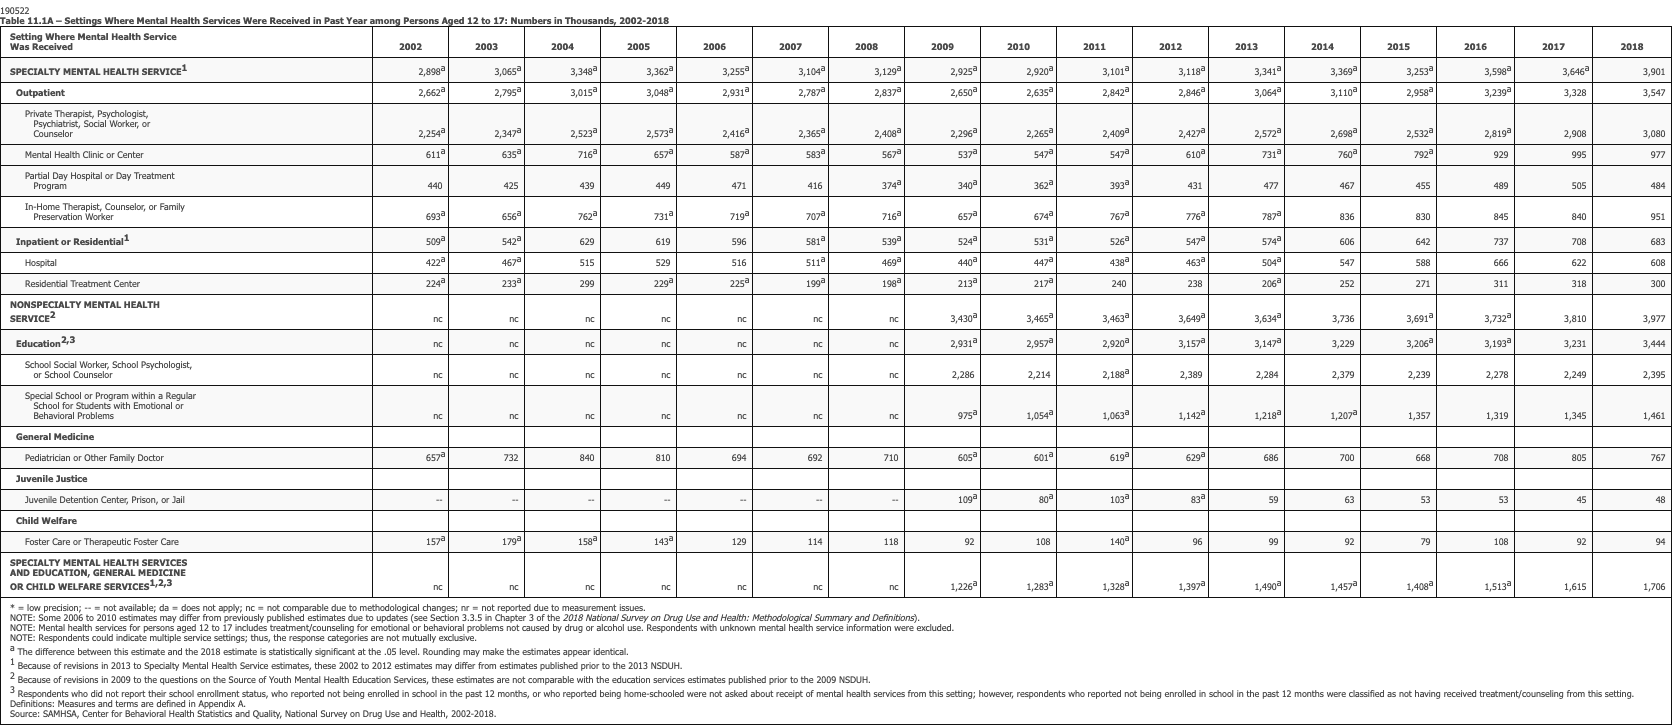
\includegraphics[width=0.9\linewidth]{/Users/carriewright/Documents/GitHub/ocs-youth-mental-health-case-study/img/table11.1a} \end{center}

First, we will add the \texttt{type} and \texttt{subtype} variables
using the \texttt{mutate} function.

\begin{Shaded}
\begin{Highlighting}[]
\NormalTok{table11}\FloatTok{.1}\NormalTok{a }\OperatorTok
\StringTok{  }\KeywordTok{mutate}\NormalTok{(}\DataTypeTok{type =} \KeywordTok{c}\NormalTok{(}\KeywordTok{rep}\NormalTok{(}\StringTok{"Specialty"}\NormalTok{, }\DecValTok{9}\NormalTok{), }
                  \KeywordTok{rep}\NormalTok{(}\StringTok{"Nonspecialty"}\NormalTok{, }\DecValTok{11}\NormalTok{))) }\OperatorTok
\StringTok{  }\KeywordTok{mutate}\NormalTok{(}\DataTypeTok{subtype =} \KeywordTok{c}\NormalTok{(}\StringTok{"Specialty_total"}\NormalTok{, }
                     \KeywordTok{rep}\NormalTok{(}\StringTok{"Outpatient"}\NormalTok{, }\DecValTok{5}\NormalTok{), }
                     \KeywordTok{rep}\NormalTok{(}\StringTok{"Inpatient"}\NormalTok{, }\DecValTok{3}\NormalTok{), }
                     \StringTok{"Nonspecialty_total"}\NormalTok{, }
                     \KeywordTok{rep}\NormalTok{(}\StringTok{"Education"}\NormalTok{, }\DecValTok{3}\NormalTok{), }
                     \KeywordTok{rep}\NormalTok{(}\StringTok{"General_medicine"}\NormalTok{, }\DecValTok{2}\NormalTok{),}
                     \KeywordTok{rep}\NormalTok{(}\StringTok{"Juvenile_Justice"}\NormalTok{, }\DecValTok{2}\NormalTok{), }
                     \KeywordTok{rep}\NormalTok{(}\StringTok{"Child_Welfare"}\NormalTok{, }\DecValTok{2}\NormalTok{), }
                     \StringTok{"combination"}\NormalTok{))}
\end{Highlighting}
\end{Shaded}

We also want to add a variable with shorter names for labels in plots
and statistical output.

\begin{Shaded}
\begin{Highlighting}[]
\NormalTok{table11}\FloatTok{.1}\NormalTok{a }\OperatorTok
\StringTok{  }\KeywordTok{mutate}\NormalTok{(}\DataTypeTok{short_label =} \KeywordTok{c}\NormalTok{(}\StringTok{"Specialty total"}\NormalTok{, }
                         \StringTok{"Outpatient total"}\NormalTok{, }
                         \StringTok{"Therapist"}\NormalTok{, }
                         \StringTok{"Clinic"}\NormalTok{, }
                         \StringTok{"Day program"}\NormalTok{,}
                         \StringTok{"In-home Therapist"}\NormalTok{, }
                         \StringTok{"Inpatient total"}\NormalTok{, }
                         \StringTok{"Hospital"}\NormalTok{, }
                         \StringTok{"Residential Center"}\NormalTok{,}
                         \StringTok{"Nonspecialty total"}\NormalTok{, }
                         \StringTok{"School total"}\NormalTok{, }
                         \StringTok{"School Therapist"}\NormalTok{, }
                         \StringTok{"School Program"}\NormalTok{, }
                         \StringTok{"General Medicine"}\NormalTok{,}
                         \StringTok{"Family Dr"}\NormalTok{,}
                         \StringTok{"Justice System"}\NormalTok{,}
                         \StringTok{"Justice System"}\NormalTok{,}
                         \StringTok{"Welfare"}\NormalTok{, }
                         \StringTok{"Fostercare"}\NormalTok{, }
                         \StringTok{"Specialty Combination"}\NormalTok{))}
\end{Highlighting}
\end{Shaded}

We can remove the empty rows using the \texttt{filter()} function of the
\texttt{dplyr} package. We can specify that we don't want to keep these
rows by using the \texttt{!=} not equal to operator.

\begin{Shaded}
\begin{Highlighting}[]
\NormalTok{table11}\FloatTok{.1}\NormalTok{a }\OperatorTok
\StringTok{  }\NormalTok{dplyr}\OperatorTok{::}\KeywordTok{filter}\NormalTok{(MHS_setting }\OperatorTok{!=}\StringTok{ "General_Medicine"}\NormalTok{) }\OperatorTok
\StringTok{  }\NormalTok{dplyr}\OperatorTok{::}\KeywordTok{filter}\NormalTok{(MHS_setting }\OperatorTok{!=}\StringTok{ "Juvenile_Justice"}\NormalTok{) }\OperatorTok
\StringTok{  }\NormalTok{dplyr}\OperatorTok{::}\KeywordTok{filter}\NormalTok{(MHS_setting }\OperatorTok{!=}\StringTok{ "Child_Welfare"}\NormalTok{)}

\KeywordTok{head}\NormalTok{(table11}\FloatTok{.1}\NormalTok{a)}
\end{Highlighting}
\end{Shaded}

\begin{verbatim}
# A tibble: 6 x 21
  MHS_setting `2002` `2003` `2004` `2005` `2006` `2007` `2008` `2009` `2010`
  <chr>        <dbl>  <dbl>  <dbl>  <dbl>  <dbl>  <dbl>  <dbl>  <dbl>  <dbl>
1 SPECIALTY ~   2898   3065   3348   3362   3255   3104   3129   2925   2920
2 Outpatient    2662   2795   3015   3048   2931   2787   2837   2650   2635
3 Private Th~   2254   2347   2523   2573   2416   2365   2408   2296   2265
4 Mental Hea~    611    635    716    657    587    583    567    537    547
5 Partial Da~    440    425    439    449    471    416    374    340    362
6 InHome The~    693    656    762    731    719    707    716    657    674
# ... with 11 more variables: `2011` <dbl>, `2012` <dbl>, `2013` <dbl>,
#   `2014` <dbl>, `2015` <dbl>, `2016` <dbl>, `2017` <dbl>, `2018` <dbl>,
#   type <chr>, subtype <chr>, short_label <chr>
\end{verbatim}

Finally, we would like to change the shape of our table so that we have
a new column that represents the year and a new column that represents
the value for that year. To do so we will be making our table
``longer'', meaning that it will have fewer columns and more rows. See
\href{https://en.wikipedia.org/wiki/Wide_and_narrow_data}{here} for more
information about different table formats, typically referred to as wide
and long or sometimes narrow.

We will use the \texttt{pivot\_longer()} function of the \texttt{tidyr}
package to change the shape of our table.

There are 3 main arguments in this function:

\begin{enumerate}
\def\labelenumi{\arabic{enumi}.}
\tightlist
\item
  \texttt{cols} - which specifies what columns to collapse\\
\item
  \texttt{names\_to} - which specifies the name of the new column that
  will be created that will contain the column names of the columns you
  are collapsing\\
\item
  \texttt{values\_to} - which specifies the name of the new column that
  will be created that will contain the values from the columns you are
  collapsing
\end{enumerate}

To specify that we want to collapse all the columns that have year
values, we can chose those that contain the string \texttt{"20"} using
the \texttt{contains()} function of \texttt{dplyr}.

Finally, we will make the \texttt{Year} variable numeric as well.

We will first use the base \texttt{dim()} function to see the dimensions
of our table before and after using \texttt{pivot\_longer()}.

\begin{Shaded}
\begin{Highlighting}[]
\KeywordTok{dim}\NormalTok{(table11}\FloatTok{.1}\NormalTok{a)}
\end{Highlighting}
\end{Shaded}

\begin{verbatim}
[1] 20 21
\end{verbatim}

\begin{Shaded}
\begin{Highlighting}[]
\NormalTok{table11}\FloatTok{.1}\NormalTok{a }\OperatorTok
\StringTok{  }\NormalTok{tidyr}\OperatorTok{::}\KeywordTok{pivot_longer}\NormalTok{(}\DataTypeTok{cols =} \KeywordTok{contains}\NormalTok{(}\StringTok{"20"}\NormalTok{), }
                      \DataTypeTok{names_to =} \StringTok{"Year"}\NormalTok{,}
                      \DataTypeTok{values_to =} \StringTok{"Number"}\NormalTok{) }\OperatorTok
\StringTok{  }\KeywordTok{mutate}\NormalTok{(}\DataTypeTok{Year =} \KeywordTok{as.numeric}\NormalTok{(Year))}

\KeywordTok{dim}\NormalTok{(table11}\FloatTok{.1}\NormalTok{a)}
\end{Highlighting}
\end{Shaded}

\begin{verbatim}
[1] 340   6
\end{verbatim}

\begin{Shaded}
\begin{Highlighting}[]
\KeywordTok{head}\NormalTok{(table11}\FloatTok{.1}\NormalTok{a)}
\end{Highlighting}
\end{Shaded}

\begin{verbatim}
# A tibble: 6 x 6
  MHS_setting                 type     subtype       short_label     Year Number
  <chr>                       <chr>    <chr>         <chr>          <dbl>  <dbl>
1 SPECIALTY MENTAL HEALTH SE~ Special~ Specialty_to~ Specialty tot~  2002   2898
2 SPECIALTY MENTAL HEALTH SE~ Special~ Specialty_to~ Specialty tot~  2003   3065
3 SPECIALTY MENTAL HEALTH SE~ Special~ Specialty_to~ Specialty tot~  2004   3348
4 SPECIALTY MENTAL HEALTH SE~ Special~ Specialty_to~ Specialty tot~  2005   3362
5 SPECIALTY MENTAL HEALTH SE~ Special~ Specialty_to~ Specialty tot~  2006   3255
6 SPECIALTY MENTAL HEALTH SE~ Special~ Specialty_to~ Specialty tot~  2007   3104
\end{verbatim}

We can see that our table is now much longer - as we have 340 rows!

\hypertarget{section-16}{%
\paragraph{}\label{section-16}}

Question Opportunity

Why do we have 340 rows now?

\hypertarget{section-17}{%
\paragraph{}\label{section-17}}

Now, we see that the \texttt{Year} and \texttt{Number} variables are of
class double because of the \texttt{\textless{}dbl\textgreater{}} under
the column name.

Let's remind ourselves what the rest of the tables contain:

\begin{longtable}[]{@{}ll@{}}
\toprule
\begin{minipage}[b]{0.18\columnwidth}\raggedright
Table\strut
\end{minipage} & \begin{minipage}[b]{0.76\columnwidth}\raggedright
Details\strut
\end{minipage}\tabularnewline
\midrule
\endhead
\begin{minipage}[t]{0.18\columnwidth}\raggedright
Table 11.1A\strut
\end{minipage} & \begin{minipage}[t]{0.76\columnwidth}\raggedright
Settings Where Mental Health Services Were Received in Past Year among
Persons Aged 12 to 17: Numbers in Thousands, 2002-2018\strut
\end{minipage}\tabularnewline
\begin{minipage}[t]{0.18\columnwidth}\raggedright
Table 11.1B\strut
\end{minipage} & \begin{minipage}[t]{0.76\columnwidth}\raggedright
Settings Where Mental Health Services Were Received in Past Year among
Persons Aged 12 to 17: Percentages, 2002-2018\strut
\end{minipage}\tabularnewline
\begin{minipage}[t]{0.18\columnwidth}\raggedright
Table 11.2A\strut
\end{minipage} & \begin{minipage}[t]{0.76\columnwidth}\raggedright
Major Depressive Episode in Past Year among Persons Aged 12 to 17, by
Demographic Characteristics: Numbers in Thousands, 2004-2018\strut
\end{minipage}\tabularnewline
\begin{minipage}[t]{0.18\columnwidth}\raggedright
Table 11.2B\strut
\end{minipage} & \begin{minipage}[t]{0.76\columnwidth}\raggedright
Major Depressive Episode in Past Year among Persons Aged 12 to 17, by
Demographic Characteristics: Percentages, 2004-2018\strut
\end{minipage}\tabularnewline
\begin{minipage}[t]{0.18\columnwidth}\raggedright
Table 11.3A\strut
\end{minipage} & \begin{minipage}[t]{0.76\columnwidth}\raggedright
Major Depressive Episode with Severe Impairment in Past Year among
Persons Aged 12 to 17, by Demographic Characteristics: Numbers in
Thousands, 2006-2018\strut
\end{minipage}\tabularnewline
\begin{minipage}[t]{0.18\columnwidth}\raggedright
Table 11.3B\strut
\end{minipage} & \begin{minipage}[t]{0.76\columnwidth}\raggedright
Major Depressive Episode with Severe Impairment in Past Year among
Persons Aged 12 to 17, by Demographic Characteristics: Percentages,
2006-2018\strut
\end{minipage}\tabularnewline
\begin{minipage}[t]{0.18\columnwidth}\raggedright
Table 11.4A\strut
\end{minipage} & \begin{minipage}[t]{0.76\columnwidth}\raggedright
Receipt of Treatment for Depression in Past Year among Persons Aged 12
to 17 with Major Depressive Episode in Past Year, by Demographic
Characteristics: Numbers in Thousands, 2004-2018\strut
\end{minipage}\tabularnewline
\begin{minipage}[t]{0.18\columnwidth}\raggedright
Table 11.4B\strut
\end{minipage} & \begin{minipage}[t]{0.76\columnwidth}\raggedright
Receipt of Treatment for Depression in Past Year among Persons Aged 12
to 17 with Major Depressive Episode in Past Year, by Demographic
Characteristics: Percentages, 2004-2018\strut
\end{minipage}\tabularnewline
\bottomrule
\end{longtable}

OK, so the next table (Table11.1B) is very similar to Table11.1A, while
the remaining tables have information about demographics.

As a reminder here are all of the steps that we performed to wrangle
\texttt{table11.1a}:

\begin{Shaded}
\begin{Highlighting}[]
\NormalTok{table11}\FloatTok{.1}\NormalTok{a }\OperatorTok
\CommentTok{# make the table into a tibble}
\StringTok{  }\NormalTok{dplyr}\OperatorTok{::}\KeywordTok{as_tibble}\NormalTok{() }\OperatorTok
\CommentTok{# remove the last row by only keeping the first through the second to last}
\StringTok{  }\KeywordTok{slice}\NormalTok{(}\DecValTok{1}\OperatorTok{:}\NormalTok{(}\KeywordTok{n}\NormalTok{() }\OperatorTok{-}\StringTok{ }\DecValTok{1}\NormalTok{)) }\OperatorTok
\CommentTok{# make the "nc" values "NA" instead}
\StringTok{  }\NormalTok{dplyr}\OperatorTok{::}\KeywordTok{na_if}\NormalTok{(}\StringTok{"nc"}\NormalTok{) }\OperatorTok
\StringTok{  }\NormalTok{dplyr}\OperatorTok{::}\KeywordTok{na_if}\NormalTok{(}\StringTok{"--"}\NormalTok{) }\OperatorTok
\StringTok{  }\NormalTok{dplyr}\OperatorTok{::}\KeywordTok{na_if}\NormalTok{(}\StringTok{""}\NormalTok{) }\OperatorTok
\StringTok{  }\NormalTok{dplyr}\OperatorTok{::}\KeywordTok{na_if}\NormalTok{(}\StringTok{"*"}\NormalTok{) }\OperatorTok\StringTok{ }
\CommentTok{# rename the column to the shorter MHS_setting name}
\StringTok{  }\NormalTok{dplyr}\OperatorTok{::}\KeywordTok{rename}\NormalTok{(}\DataTypeTok{MHS_setting =} 
                  \StringTok{`}\DataTypeTok{Setting Where Mental Health ServiceWas Received}\StringTok{`}\NormalTok{) }\OperatorTok
\CommentTok{# remove numbers, carriage return, new lines, and punctuation marks from the values for the MHS_setting column}
\StringTok{  }\KeywordTok{mutate}\NormalTok{(}\DataTypeTok{MHS_setting =} 
         \KeywordTok{str_remove_all}\NormalTok{(}\DataTypeTok{string =}\NormalTok{ MHS_setting, }
                       \DataTypeTok{pattern =} \StringTok{"[:digit:]|}\CharTok{\textbackslash{}r\textbackslash{}n}\StringTok{|[:punct:]|"}\NormalTok{)) }\OperatorTok
\CommentTok{# replace the white spaces with a single space}
\StringTok{  }\KeywordTok{mutate}\NormalTok{(}\DataTypeTok{MHS_setting =} 
         \KeywordTok{str_replace_all}\NormalTok{(}\DataTypeTok{string =}\NormalTok{ MHS_setting,}
                        \DataTypeTok{pattern =} \StringTok{"[:blank:]\{1,\}"}\NormalTok{, }
                    \DataTypeTok{replacement =} \StringTok{" "}\NormalTok{)) }\OperatorTok
\CommentTok{# remove "a" and commas from the values in the columns except the column called MHS_setting}
\StringTok{  }\KeywordTok{mutate}\NormalTok{(dplyr}\OperatorTok{::}\KeywordTok{across}\NormalTok{(}\DataTypeTok{.cols =} \OperatorTok{-}\NormalTok{MHS_setting,}
\NormalTok{                stringr}\OperatorTok{::}\NormalTok{str_remove_all, }\StringTok{"a|,"}\NormalTok{)) }\OperatorTok
\CommentTok{# make those columns numeric}
\StringTok{  }\KeywordTok{mutate}\NormalTok{(}\KeywordTok{across}\NormalTok{(}\OperatorTok{-}\NormalTok{MHS_setting, as.numeric)) }\OperatorTok
\CommentTok{# create a new type column with the values: "Specialty repeated 9 times followed by "Nonspecialty" repeated 11 times}
\StringTok{  }\KeywordTok{mutate}\NormalTok{(}\DataTypeTok{type =} \KeywordTok{c}\NormalTok{(}\KeywordTok{rep}\NormalTok{(}\StringTok{"Specialty"}\NormalTok{, }\DecValTok{9}\NormalTok{), }\KeywordTok{rep}\NormalTok{(}\StringTok{"Nonspecialty"}\NormalTok{, }\DecValTok{11}\NormalTok{))) }\OperatorTok
\CommentTok{# create a new variable called subtype }
\StringTok{  }\KeywordTok{mutate}\NormalTok{(}\DataTypeTok{subtype =}\KeywordTok{c}\NormalTok{(}\StringTok{"Specialty_total"}\NormalTok{, }
                    \KeywordTok{rep}\NormalTok{(}\StringTok{"Outpatient"}\NormalTok{, }\DecValTok{5}\NormalTok{), }
                    \KeywordTok{rep}\NormalTok{(}\StringTok{"Inpatient"}\NormalTok{, }\DecValTok{3}\NormalTok{), }
                    \StringTok{"Nonspecialty_total"}\NormalTok{, }
                    \KeywordTok{rep}\NormalTok{(}\StringTok{"Education"}\NormalTok{, }\DecValTok{3}\NormalTok{), }
                    \KeywordTok{rep}\NormalTok{(}\StringTok{"General_medicine"}\NormalTok{, }\DecValTok{2}\NormalTok{),}
                    \KeywordTok{rep}\NormalTok{(}\StringTok{"Juvenile_Justice"}\NormalTok{, }\DecValTok{2}\NormalTok{),}
                    \KeywordTok{rep}\NormalTok{(}\StringTok{"Child_Welfare"}\NormalTok{, }\DecValTok{2}\NormalTok{), }
                    \StringTok{"combination"}\NormalTok{)) }\OperatorTok
\CommentTok{# create a new variabel called short_label}
\StringTok{  }\KeywordTok{mutate}\NormalTok{(}\DataTypeTok{short_label =} \KeywordTok{c}\NormalTok{(}\StringTok{"Specialty total"}\NormalTok{, }\StringTok{"Outpatient total"}\NormalTok{,}
                         \StringTok{"Therapist"}\NormalTok{, }\StringTok{"Clinic"}\NormalTok{, }\StringTok{"Day program"}\NormalTok{, }
                         \StringTok{"In-home Therapist"}\NormalTok{, }\StringTok{"Inpatient total"}\NormalTok{,}
                         \StringTok{"Hospital"}\NormalTok{, }\StringTok{"Residential Center"}\NormalTok{,}
                         \StringTok{"Nonspecialty total"}\NormalTok{, }\StringTok{"School total"}\NormalTok{, }
                         \StringTok{"School Therapist"}\NormalTok{, }\StringTok{"School Program"}\NormalTok{, }
                         \StringTok{"General Medicine"}\NormalTok{, }\StringTok{"Family Dr"}\NormalTok{, }
                         \StringTok{"Justice System"}\NormalTok{, }\StringTok{"Justice System"}\NormalTok{,}
                         \StringTok{"Welfare"}\NormalTok{, }\StringTok{"Fostercare"}\NormalTok{, }
                         \StringTok{"Specialty Combination"}\NormalTok{)) }\OperatorTok
\CommentTok{# remove rows with General_Medicine as the value in the MHS_setting column because it is empty}
\StringTok{  }\NormalTok{dplyr}\OperatorTok{::}\KeywordTok{filter}\NormalTok{(MHS_setting }\OperatorTok{!=}\StringTok{ "General_Medicine"}\NormalTok{) }\OperatorTok
\CommentTok{# remove rows with Juvenile_Justice as the value in the MHS_setting column because it is empty}
\StringTok{  }\NormalTok{dplyr}\OperatorTok{::}\KeywordTok{filter}\NormalTok{(MHS_setting }\OperatorTok{!=}\StringTok{ "Juvenile_Justice"}\NormalTok{) }\OperatorTok
\CommentTok{# remove rows with Child_Welfare as the value in the MHS_setting column because it is empty}
\StringTok{  }\NormalTok{dplyr}\OperatorTok{::}\KeywordTok{filter}\NormalTok{(MHS_setting }\OperatorTok{!=}\StringTok{ "Child_Welfare"}\NormalTok{) }\OperatorTok
\CommentTok{# make the table in long format}
\StringTok{    }\NormalTok{tidyr}\OperatorTok{::}\KeywordTok{pivot_longer}\NormalTok{(}\DataTypeTok{cols =} \KeywordTok{contains}\NormalTok{(}\StringTok{"20"}\NormalTok{),}
                        \DataTypeTok{names_to =} \StringTok{"Year"}\NormalTok{,}
                        \DataTypeTok{values_to =} \StringTok{"Number"}\NormalTok{) }\OperatorTok
\CommentTok{# make the new Year variable to be numeric}
\StringTok{   }\KeywordTok{mutate}\NormalTok{(}\DataTypeTok{Year =} \KeywordTok{as.numeric}\NormalTok{(Year))}
\end{Highlighting}
\end{Shaded}

Now we want to wrangle table11.1B which is formatted the most similarly.
To do so we can simply run these steps on the using the
\texttt{table11.1B} as the input. For the sake of education, however, we
will show you how you could make a function if we had several more
similar tables to wrangle. This will also make it easier to write a
function to wrangle the other demographic tables.

Last time we wrote a function in this case study, we only had one input
in our function. This time we will have several inputs. We will have the
table that we want to wrangle as \texttt{TABLE}, a new name for the
first column called \texttt{new\_col}, and an input called
\texttt{pivot\_col}, which will be the name of the column that will be
created after pivoting that will take the values from each of the years.

\begin{Shaded}
\begin{Highlighting}[]
\ControlFlowTok{function}\NormalTok{(TABLE, new_col, pivot_col)\{}
    \OperatorTok{<}\NormalTok{add code here}\OperatorTok{>}\StringTok{ }
\StringTok{  }\NormalTok{\}}
\end{Highlighting}
\end{Shaded}

We want to make our function flexible so that it can take any value for
the name of the first column. To select the first column we will use
this following code, where the base \texttt{names()} function gets the
column names of the \texttt{TABLE} input , which is indicated by the
\texttt{.} and then to get just the first name the \texttt{{[}1{]}} is
used.

\begin{Shaded}
\begin{Highlighting}[]
\ControlFlowTok{function}\NormalTok{(TABLE, new_col, pivot_col)\{}
\NormalTok{  dplyr}\OperatorTok{::}\KeywordTok{as_tibble}\NormalTok{(TABLE) }\OperatorTok
\StringTok{  }\CommentTok{#additional steps}
\StringTok{  }\KeywordTok{names}\NormalTok{(.)[}\DecValTok{1}\NormalTok{]}
  \CommentTok{#additional steps}
\NormalTok{\}}
\end{Highlighting}
\end{Shaded}

And to rename the with the \texttt{new\_col} input to the function we
can do this:

\begin{Shaded}
\begin{Highlighting}[]
\ControlFlowTok{function}\NormalTok{(TABLE, new_col, pivot_col)\{}
\NormalTok{  dplyr}\OperatorTok{::}\KeywordTok{as_tibble}\NormalTok{(TABLE) }\OperatorTok
\StringTok{  }\CommentTok{#additional steps}
\StringTok{  }\KeywordTok{rename}\NormalTok{(\{\{new_col\}\} }\OperatorTok{:}\ErrorTok{=}\StringTok{ }\KeywordTok{names}\NormalTok{(.)[}\DecValTok{1}\NormalTok{])}
  \CommentTok{#additional steps}
\NormalTok{\}}
\end{Highlighting}
\end{Shaded}

The double curly brackets \texttt{\{\{\}\}} allow us to use the input to
the function called \texttt{new\_col} within the function.

See \href{https://adv-r.hadley.nz/quasiquotation.html\#tidy-dots}{here}
for information about the \texttt{:=} colon-equals operator. This
operator is more flexible than the normal \texttt{=}. It allows
expressions on both sides, thus it allows us to use an expression (the
values for \texttt{new\_col}) as the input value to the expressions that
follow the \texttt{:=} operator.

We will also add code to remove all rows that have only \texttt{NA}
values in a more flexible way, so that we don't need to know what rows
ahead of time.

To do this we will use the \texttt{filter()} and \texttt{select()}
functions of the \texttt{dplyr} package.

We will calculate a sum of the count of \texttt{NA} values across the
rows for the columns for each year using the base \texttt{rowSums()}
function like so:

\begin{Shaded}
\begin{Highlighting}[]
\KeywordTok{rowSums}\NormalTok{(}\KeywordTok{is.na}\NormalTok{(.))}
\end{Highlighting}
\end{Shaded}

However to do this we first need to select only the columns that are
numeric using: \texttt{select(.,\ is.numeric)}, where the \texttt{.}
refers to the table after all the previous wrangling steps in our
function. Importantly of course, this all needs to happen after we
convert the values for each year to numeric.

Anyway, altogether this looks like this:

\begin{Shaded}
\begin{Highlighting}[]
\KeywordTok{rowSums}\NormalTok{(}\KeywordTok{is.na}\NormalTok{(}\KeywordTok{select}\NormalTok{(., is.numeric)))}\StringTok{`}\DataTypeTok{.}
\end{Highlighting}
\end{Shaded}

Finally, we compare this to the number of columns that are numeric by
using: \texttt{length(select(.,\ is.numeric)))}, with the idea that if
the number of \texttt{NA} values is less than the number of columns that
could have \texttt{NA} values, then we know it is not an empty row.

Overall, this would look something like this after we perform a step to
convert the columns to be numeric like we did before:

\begin{Shaded}
\begin{Highlighting}[]
\ControlFlowTok{function}\NormalTok{(TABLE, new_col, pivot_col)\{}
  \CommentTok{# previous similar steps to modify and make table values numeric}
    \KeywordTok{filter}\NormalTok{(}\KeywordTok{rowSums}\NormalTok{(}\KeywordTok{is.na}\NormalTok{(}\KeywordTok{select}\NormalTok{(., is.numeric))) }\OperatorTok{<}\StringTok{ }
\StringTok{             }\KeywordTok{length}\NormalTok{(}\KeywordTok{select}\NormalTok{(., is.numeric))) }
\NormalTok{  \}}
\end{Highlighting}
\end{Shaded}

Note that if we were using the \texttt{summarize()} or \texttt{mutate()}
function or the \texttt{dplyr} package, then we could use the
\texttt{across()} function of the \texttt{dplyr} package to select what
columns we wanted to use in our calculation.

OK, so putting everything together from what we did previously for
\texttt{table11.1a} and these new flexible steps we can create this
function:

\begin{Shaded}
\begin{Highlighting}[]
\NormalTok{data_prep_settings <-}\StringTok{ }\ControlFlowTok{function}\NormalTok{(TABLE, new_col, pivot_col)\{}
\CommentTok{# make the table a tibble}
\NormalTok{  dplyr}\OperatorTok{::}\KeywordTok{as_tibble}\NormalTok{(TABLE) }\OperatorTok
\CommentTok{# remove the last row}
\StringTok{    }\KeywordTok{slice}\NormalTok{(}\DecValTok{1}\OperatorTok{:}\NormalTok{(}\KeywordTok{n}\NormalTok{() }\OperatorTok{-}\StringTok{ }\DecValTok{1}\NormalTok{)) }\OperatorTok
\CommentTok{# make "nc" values NA etc.}
\StringTok{    }\KeywordTok{na_if}\NormalTok{(}\StringTok{"nc"}\NormalTok{) }\OperatorTok
\StringTok{    }\KeywordTok{na_if}\NormalTok{(}\StringTok{"--"}\NormalTok{) }\OperatorTok
\StringTok{    }\KeywordTok{na_if}\NormalTok{(}\StringTok{""}\NormalTok{) }\OperatorTok
\StringTok{    }\KeywordTok{na_if}\NormalTok{(}\StringTok{"*"}\NormalTok{) }\OperatorTok\StringTok{ }
\CommentTok{# rename the first column (names(.)[1]) to be what was specified with the new_col argument}
\StringTok{    }\KeywordTok{rename}\NormalTok{(\{\{new_col\}\} }\OperatorTok{:}\ErrorTok{=}\StringTok{ }\KeywordTok{names}\NormalTok{(.)[}\DecValTok{1}\NormalTok{]) }\OperatorTok
\CommentTok{# remove the numbers and punctuation marks and carriage returns (\textbackslash{}r) and new lines (\textbackslash{}n) from the first column}
\StringTok{    }\KeywordTok{mutate}\NormalTok{(\{\{new_col\}\} }\OperatorTok{:}\ErrorTok{=}\StringTok{ }
\StringTok{        }\KeywordTok{str_remove_all}\NormalTok{(}\DataTypeTok{string =} \KeywordTok{pull}\NormalTok{(., \{\{new_col\}\}), }
                        \DataTypeTok{pattern =} \StringTok{"[:digit:]|}\CharTok{\textbackslash{}r\textbackslash{}n}\StringTok{|[:punct:]|"}\NormalTok{)) }\OperatorTok
\CommentTok{# replace white spaces with a single space}
\StringTok{    }\KeywordTok{mutate}\NormalTok{(\{\{new_col\}\} }\OperatorTok{:}\ErrorTok{=}\StringTok{ }
\StringTok{        }\KeywordTok{str_replace_all}\NormalTok{(}\DataTypeTok{string =}\KeywordTok{pull}\NormalTok{(., \{\{new_col\}\}),}
                         \DataTypeTok{pattern =} \StringTok{"[:blank:]\{1,\}"}\NormalTok{, }
                         \DataTypeTok{replacement =} \StringTok{" "}\NormalTok{)) }\OperatorTok
\CommentTok{# remove "a" and , from the values for the columns that are not the first column (called new_col)}
\StringTok{    }\KeywordTok{mutate}\NormalTok{(dplyr}\OperatorTok{::}\KeywordTok{across}\NormalTok{(}\DataTypeTok{.cols =} \OperatorTok{-}\NormalTok{\{\{new_col\}\},}
\NormalTok{                       stringr}\OperatorTok{::}\NormalTok{str_remove_all, }\StringTok{"a|,"}\NormalTok{)) }\OperatorTok
\CommentTok{# make these columns numeric  (all the columns but the first column)}
\StringTok{    }\KeywordTok{mutate}\NormalTok{(}\KeywordTok{across}\NormalTok{(}\OperatorTok{-}\NormalTok{\{\{new_col\}\}, as.numeric)) }\OperatorTok
\CommentTok{# make a new variable called type with 9 values that are Specialty followed by 11 values of Nonspecialty}
\StringTok{    }\KeywordTok{mutate}\NormalTok{(}\DataTypeTok{type =} \KeywordTok{c}\NormalTok{(}\KeywordTok{rep}\NormalTok{(}\StringTok{"Specialty"}\NormalTok{, }\DecValTok{9}\NormalTok{), }\KeywordTok{rep}\NormalTok{(}\StringTok{"Nonspecialty"}\NormalTok{, }\DecValTok{11}\NormalTok{))) }\OperatorTok
\CommentTok{# make a new variable called subtype with the following values repeated various times}
\StringTok{    }\KeywordTok{mutate}\NormalTok{(}\DataTypeTok{subtype =} \KeywordTok{c}\NormalTok{(}\StringTok{"Specialty_total"}\NormalTok{,}
                       \KeywordTok{rep}\NormalTok{(}\StringTok{"Outpatient"}\NormalTok{, }\DecValTok{5}\NormalTok{),}
                       \KeywordTok{rep}\NormalTok{(}\StringTok{"Inpatient"}\NormalTok{, }\DecValTok{3}\NormalTok{),}
                       \StringTok{"Nonspecialty_total"}\NormalTok{,}
                       \KeywordTok{rep}\NormalTok{(}\StringTok{"Education"}\NormalTok{, }\DecValTok{3}\NormalTok{),}
                       \KeywordTok{rep}\NormalTok{(}\StringTok{"General_medicine"}\NormalTok{, }\DecValTok{2}\NormalTok{),}
                       \KeywordTok{rep}\NormalTok{(}\StringTok{"Juvenile_Justice"}\NormalTok{, }\DecValTok{2}\NormalTok{),}
                       \KeywordTok{rep}\NormalTok{(}\StringTok{"Child_Welfare"}\NormalTok{, }\DecValTok{2}\NormalTok{),}
                       \StringTok{"combination"}\NormalTok{)) }\OperatorTok\StringTok{ }
\CommentTok{# make a new variable called short_label to use as labels for plots for the data}
\StringTok{    }\KeywordTok{mutate}\NormalTok{(}\DataTypeTok{short_label =} \KeywordTok{c}\NormalTok{(}\StringTok{"Specialty total"}\NormalTok{, }\StringTok{"Outpatient total"}\NormalTok{,  }
                           \StringTok{"Therapist"}\NormalTok{, }\StringTok{"Clinic"}\NormalTok{, }\StringTok{"Day program"}\NormalTok{, }
                           \StringTok{"In-home Therapist"}\NormalTok{, }\StringTok{"Inpatient total"}\NormalTok{,}
                           \StringTok{"Hospital"}\NormalTok{, }\StringTok{"Residential Center"}\NormalTok{,}
                           \StringTok{"Nonspecialty total"}\NormalTok{, }\StringTok{"School total"}\NormalTok{, }
                           \StringTok{"School Therapist"}\NormalTok{, }\StringTok{"School Program"}\NormalTok{, }
                           \StringTok{"General Medicine"}\NormalTok{, }\StringTok{"Family Dr"}\NormalTok{, }
                           \StringTok{"Justice System"}\NormalTok{, }\StringTok{"Justice System"}\NormalTok{, }
                           \StringTok{"Welfare"}\NormalTok{, }\StringTok{"Fostercare"}\NormalTok{, }
                           \StringTok{"Specialty Combination"}\NormalTok{)) }\OperatorTok
\CommentTok{# remove rows were all the values are NA - }
\CommentTok{# the number of `NA` values for a row should be less than the number of columns that could have `NA` values}
\StringTok{  }\KeywordTok{filter}\NormalTok{(}\KeywordTok{rowSums}\NormalTok{(}\KeywordTok{is.na}\NormalTok{(}\KeywordTok{select}\NormalTok{(., is.numeric))) }\OperatorTok{<}
\StringTok{           }\KeywordTok{length}\NormalTok{(}\KeywordTok{select}\NormalTok{(., is.numeric))) }\OperatorTok
\CommentTok{# make the table into long format so that the year columns are collapsed together }
\CommentTok{# the new value column is called what was specified with the "pivot_col" argument}
\StringTok{  }\KeywordTok{pivot_longer}\NormalTok{(}\DataTypeTok{cols =} \KeywordTok{contains}\NormalTok{(}\StringTok{"20"}\NormalTok{),}
               \DataTypeTok{names_to =} \StringTok{"Year"}\NormalTok{, }
               \DataTypeTok{values_to =}\NormalTok{ pivot_col)}\OperatorTok
\CommentTok{# make the new "Year" variable numeric}
\StringTok{  }\KeywordTok{mutate}\NormalTok{(}\DataTypeTok{Year =} \KeywordTok{as.numeric}\NormalTok{(Year))}
\NormalTok{\}}
\end{Highlighting}
\end{Shaded}

Now we can apply the function to \texttt{table11.1b}.

\hypertarget{table11.1b}{%
\subsubsection{\texorpdfstring{\textbf{Table11.1b}}{Table11.1b}}\label{table11.1b}}

\begin{center}\rule{0.5\linewidth}{0.5pt}\end{center}

\begin{Shaded}
\begin{Highlighting}[]
\NormalTok{table11}\FloatTok{.1}\NormalTok{b <-}\StringTok{ }
\StringTok{  }\KeywordTok{data_prep_settings}\NormalTok{(}\DataTypeTok{TABLE =}\NormalTok{ table11}\FloatTok{.1}\NormalTok{b, }
                     \DataTypeTok{new_col =} \StringTok{"MHS_setting"}\NormalTok{,}
                     \DataTypeTok{pivot_col =} \StringTok{"Percent"}\NormalTok{)}

\KeywordTok{head}\NormalTok{(table11}\FloatTok{.1}\NormalTok{b)}
\end{Highlighting}
\end{Shaded}

\begin{verbatim}
# A tibble: 6 x 6
  MHS_setting                type     subtype       short_label     Year Percent
  <chr>                      <chr>    <chr>         <chr>          <dbl>   <dbl>
1 SPECIALTY MENTAL HEALTH S~ Special~ Specialty_to~ Specialty tot~  2002    11.8
2 SPECIALTY MENTAL HEALTH S~ Special~ Specialty_to~ Specialty tot~  2003    12.4
3 SPECIALTY MENTAL HEALTH S~ Special~ Specialty_to~ Specialty tot~  2004    13.4
4 SPECIALTY MENTAL HEALTH S~ Special~ Specialty_to~ Specialty tot~  2005    13.4
5 SPECIALTY MENTAL HEALTH S~ Special~ Specialty_to~ Specialty tot~  2006    13  
6 SPECIALTY MENTAL HEALTH S~ Special~ Specialty_to~ Specialty tot~  2007    12.4
\end{verbatim}

Now we have tidy data about the counts and percentages of where youths,
who experienced a major depressive episode, received treatment for
depression.

What about the subsequent tables?

\hypertarget{demographic-tables}{%
\subsubsection{\texorpdfstring{\textbf{Demographic
Tables}}{Demographic Tables}}\label{demographic-tables}}

\begin{center}\rule{0.5\linewidth}{0.5pt}\end{center}

All of the rest of the tables have demographic information and have this
general structure:

\begin{center}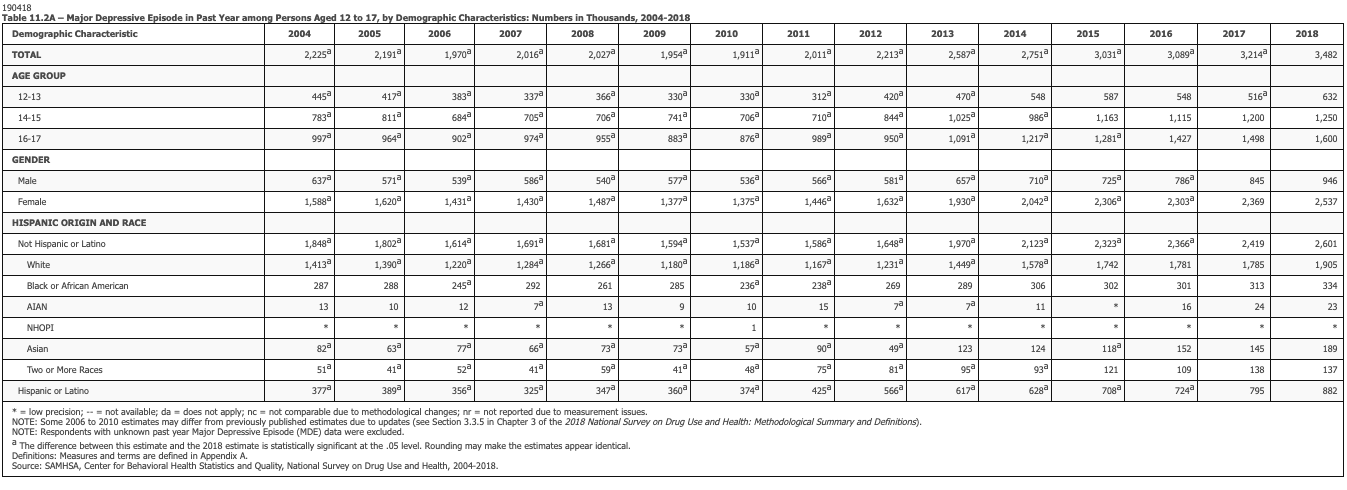
\includegraphics[width=0.9\linewidth]{/Users/carriewright/Documents/GitHub/ocs-youth-mental-health-case-study/img/dem_table} \end{center}

In these tables, we have age groups in our first column so we don't want
to remove digits or punctuation marks anymore so we need to modify our
function a bit to remove that step.

We also want to add the word \texttt{Age} and an underscore in front of
the age group listed in the tables. We can use the
\texttt{str\_replace()} function of the \texttt{stringr} package,
because now we want to only replace the first instance of \texttt{1}
with \texttt{Age:\ 1}.

We will replace the first column name with \texttt{Demographic} for all
of the tables.

We will create a new variable that list the subgroups.

We will also want to only wrangle the data up to the point that we
change the shape of the data, so that we can check how the data looks
first.

OK let's put this all together into a \texttt{data\_dem\_settings()}
function:

\begin{Shaded}
\begin{Highlighting}[]
\NormalTok{data_dem_settings <-}\StringTok{ }\ControlFlowTok{function}\NormalTok{(TABLE)\{}
  \CommentTok{# make the table a tibble}
\NormalTok{  dplyr}\OperatorTok{::}\KeywordTok{as_tibble}\NormalTok{(TABLE) }\OperatorTok
\StringTok{  }\CommentTok{# Remove the last row - keep only the 1st through 2nd to last rows}
\StringTok{  }\KeywordTok{slice}\NormalTok{(}\DecValTok{1}\OperatorTok{:}\NormalTok{(}\KeywordTok{n}\NormalTok{()}\OperatorTok{-}\DecValTok{1}\NormalTok{)) }\OperatorTok
\StringTok{  }\CommentTok{# change the values from "nc, --" etc to NA}
\StringTok{  }\KeywordTok{na_if}\NormalTok{(}\StringTok{"nc"}\NormalTok{) }\OperatorTok
\StringTok{  }\KeywordTok{na_if}\NormalTok{(}\StringTok{"--"}\NormalTok{) }\OperatorTok
\StringTok{  }\KeywordTok{na_if}\NormalTok{(}\StringTok{""}\NormalTok{) }\OperatorTok
\StringTok{  }\KeywordTok{na_if}\NormalTok{(}\StringTok{"*"}\NormalTok{) }\OperatorTok
\StringTok{  }\CommentTok{# rename the first column to be "Demographic"}
\StringTok{  }\KeywordTok{rename}\NormalTok{(}\DataTypeTok{Demographic :=} \KeywordTok{names}\NormalTok{(.)[}\DecValTok{1}\NormalTok{]) }\OperatorTok
\StringTok{  }\CommentTok{# replace white spaces form the values of the "Demographic" variable with a single space}
\StringTok{  }\KeywordTok{mutate}\NormalTok{(}\DataTypeTok{Demographic :=} \KeywordTok{str_replace_all}\NormalTok{(}\DataTypeTok{string =} \KeywordTok{pull}\NormalTok{(., Demographic),}
                                        \DataTypeTok{pattern =} \StringTok{"[:blank:]\{1,\}"}\NormalTok{, }
                                        \DataTypeTok{replacement =} \StringTok{" "}\NormalTok{)) }\OperatorTok
\StringTok{  }\CommentTok{# replace values where there is a "1" in the "Demographic" variable to be "Age: 1"}
\StringTok{  }\KeywordTok{mutate}\NormalTok{(}\DataTypeTok{Demographic =} \KeywordTok{str_replace}\NormalTok{(}\DataTypeTok{string =}\NormalTok{ Demographic, }
                                   \DataTypeTok{pattern =} \StringTok{"1"}\NormalTok{, }
                                   \DataTypeTok{replacement =} \StringTok{"Age: 1"}\NormalTok{)) }\OperatorTok
\StringTok{  }\CommentTok{# create a new variable called subgroup}
\StringTok{  }\KeywordTok{mutate}\NormalTok{(}\DataTypeTok{subgroup =} \KeywordTok{c}\NormalTok{(}\StringTok{"Total"}\NormalTok{, }\KeywordTok{rep}\NormalTok{(}\StringTok{"Age"}\NormalTok{, }\DecValTok{4}\NormalTok{), }
                    \KeywordTok{rep}\NormalTok{(}\StringTok{"Gender"}\NormalTok{, }\DecValTok{3}\NormalTok{), }\KeywordTok{rep}\NormalTok{(}\StringTok{"Race/Ethnicity"}\NormalTok{, }\DecValTok{9}\NormalTok{))) }\OperatorTok
\StringTok{  }\CommentTok{# remove "a" and commas from the variables that have column names with "20" in them}
\StringTok{  }\KeywordTok{mutate}\NormalTok{(dplyr}\OperatorTok{::}\KeywordTok{across}\NormalTok{(}\DataTypeTok{.cols =} \KeywordTok{contains}\NormalTok{(}\StringTok{"20"}\NormalTok{),}
\NormalTok{                       stringr}\OperatorTok{::}\NormalTok{str_remove_all, }\StringTok{"a|,"}\NormalTok{)) }\OperatorTok
\StringTok{  }\CommentTok{# make the variables with "20" in the names (the year variables) to be numeric}
\StringTok{  }\KeywordTok{mutate}\NormalTok{(}\KeywordTok{across}\NormalTok{(}\KeywordTok{contains}\NormalTok{(}\StringTok{"20"}\NormalTok{), as.numeric)) }\OperatorTok
\StringTok{  }\CommentTok{# remove empty rows - rows were the number of NA values is equal to the number of numeric columns}
\StringTok{  }\KeywordTok{filter}\NormalTok{(}\KeywordTok{rowSums}\NormalTok{(}\KeywordTok{is.na}\NormalTok{(}\KeywordTok{select}\NormalTok{(., is.numeric))) }\OperatorTok{<}\StringTok{ }\KeywordTok{length}\NormalTok{(}\KeywordTok{select}\NormalTok{(., is.numeric)))}
\NormalTok{  \}}
\end{Highlighting}
\end{Shaded}

Now, we use the \texttt{data\_dem\_settings()} function to wrangle the
next set of tables. We will also add a column to describe what the data
are about which will be helpful for merging the data later.

\begin{Shaded}
\begin{Highlighting}[]
\NormalTok{table11}\FloatTok{.2}\NormalTok{a <-}\StringTok{ }\KeywordTok{data_dem_settings}\NormalTok{(}\DataTypeTok{TABLE =}\NormalTok{ table11}\FloatTok{.2}\NormalTok{a)}
\NormalTok{table11}\FloatTok{.2}\NormalTok{a }\OperatorTok\StringTok{ }\KeywordTok{mutate}\NormalTok{(}\DataTypeTok{data_type =} \StringTok{"Major_Depressive_Episode"}\NormalTok{)}
\KeywordTok{head}\NormalTok{(table11}\FloatTok{.2}\NormalTok{a)}
\end{Highlighting}
\end{Shaded}

\begin{verbatim}
# A tibble: 6 x 18
  Demographic `2004` `2005` `2006` `2007` `2008` `2009` `2010` `2011` `2012`
  <chr>        <dbl>  <dbl>  <dbl>  <dbl>  <dbl>  <dbl>  <dbl>  <dbl>  <dbl>
1 TOTAL         2225   2191   1970   2016   2027   1954   1911   2011   2213
2 Age: 12-13     445    417    383    337    366    330    330    312    420
3 Age: 14-15     783    811    684    705    706    741    706    710    844
4 Age: 16-17     997    964    902    974    955    883    876    989    950
5 Male           637    571    539    586    540    577    536    566    581
6 Female        1588   1620   1431   1430   1487   1377   1375   1446   1632
# ... with 8 more variables: `2013` <dbl>, `2014` <dbl>, `2015` <dbl>,
#   `2016` <dbl>, `2017` <dbl>, `2018` <dbl>, subgroup <chr>, data_type <chr>
\end{verbatim}

\begin{Shaded}
\begin{Highlighting}[]
\NormalTok{table11}\FloatTok{.2}\NormalTok{b <-}\StringTok{ }\KeywordTok{data_dem_settings}\NormalTok{(}\DataTypeTok{TABLE =}\NormalTok{ table11}\FloatTok{.2}\NormalTok{b)}
\NormalTok{table11}\FloatTok{.2}\NormalTok{b }\OperatorTok\StringTok{ }\KeywordTok{mutate}\NormalTok{(}\DataTypeTok{data_type =} \StringTok{"Major_Depressive_Episode"}\NormalTok{)}
\KeywordTok{head}\NormalTok{(table11}\FloatTok{.2}\NormalTok{b)}
\end{Highlighting}
\end{Shaded}

\begin{verbatim}
# A tibble: 6 x 18
  Demographic `2004` `2005` `2006` `2007` `2008` `2009` `2010` `2011` `2012`
  <chr>        <dbl>  <dbl>  <dbl>  <dbl>  <dbl>  <dbl>  <dbl>  <dbl>  <dbl>
1 TOTAL          9      8.8    7.9    8.2    8.3    8.1    8      8.2    9.1
2 Age: 12-13     5.4    5.2    4.9    4.3    4.9    4.6    4.3    4.1    5.4
3 Age: 14-15     9.2    9.5    7.9    8.4    8.5    8.8    9      8.6   10.2
4 Age: 16-17    12.3   11.5   10.7   11.5   11.2   10.4   10.6   11.7   11.4
5 Male           5      4.5    4.2    4.6    4.3    4.7    4.4    4.5    4.7
6 Female        13.1   13.3   11.8   11.9   12.5   11.7   11.9   12.1   13.7
# ... with 8 more variables: `2013` <dbl>, `2014` <dbl>, `2015` <dbl>,
#   `2016` <dbl>, `2017` <dbl>, `2018` <dbl>, subgroup <chr>, data_type <chr>
\end{verbatim}

\begin{Shaded}
\begin{Highlighting}[]
\NormalTok{table11}\FloatTok{.3}\NormalTok{a <-}\StringTok{ }\KeywordTok{data_dem_settings}\NormalTok{(}\DataTypeTok{TABLE =}\NormalTok{ table11}\FloatTok{.3}\NormalTok{a)}
\NormalTok{table11}\FloatTok{.3}\NormalTok{a }\OperatorTok\StringTok{ }\KeywordTok{mutate}\NormalTok{(}\DataTypeTok{data_type =} \StringTok{"Severe_Major_Depressive_Episode"}\NormalTok{)}
\KeywordTok{head}\NormalTok{(table11}\FloatTok{.3}\NormalTok{a)}
\end{Highlighting}
\end{Shaded}

\begin{verbatim}
# A tibble: 6 x 16
  Demographic `2006` `2007` `2008` `2009` `2010` `2011` `2012` `2013` `2014`
  <chr>        <dbl>  <dbl>  <dbl>  <dbl>  <dbl>  <dbl>  <dbl>  <dbl>  <dbl>
1 TOTAL         1358   1371   1460   1404   1350   1388   1544   1868   1990
2 Age: 12-13     211    200    239    235    232    218    285    314    375
3 Age: 14-15     518    500    505    521    479    487    590    752    707
4 Age: 16-17     629    671    716    648    639    683    669    801    909
5 Male           335    386    359    391    395    397    373    435    461
6 Female        1023    986   1101   1013    954    991   1172   1432   1529
# ... with 6 more variables: `2015` <dbl>, `2016` <dbl>, `2017` <dbl>,
#   `2018` <dbl>, subgroup <chr>, data_type <chr>
\end{verbatim}

\begin{Shaded}
\begin{Highlighting}[]
\NormalTok{table11}\FloatTok{.3}\NormalTok{b <-}\StringTok{ }\KeywordTok{data_dem_settings}\NormalTok{(}\DataTypeTok{TABLE =}\NormalTok{ table11}\FloatTok{.3}\NormalTok{b)}
\NormalTok{table11}\FloatTok{.3}\NormalTok{b }\OperatorTok\StringTok{ }\KeywordTok{mutate}\NormalTok{(}\DataTypeTok{data_type =} \StringTok{"Severe_Major_Depressive_Episode"}\NormalTok{)}
\KeywordTok{head}\NormalTok{(table11}\FloatTok{.3}\NormalTok{b)}
\end{Highlighting}
\end{Shaded}

\begin{verbatim}
# A tibble: 6 x 16
  Demographic `2006` `2007` `2008` `2009` `2010` `2011` `2012` `2013` `2014`
  <chr>        <dbl>  <dbl>  <dbl>  <dbl>  <dbl>  <dbl>  <dbl>  <dbl>  <dbl>
1 TOTAL          5.5    5.5    6      5.8    5.7    5.7    6.3    7.7    8.2
2 Age: 12-13     2.7    2.5    3.2    3.2    3      2.8    3.7    4.1    4.9
3 Age: 14-15     6      6      6.1    6.2    6.1    5.9    7.1    9.1    8.5
4 Age: 16-17     7.5    7.9    8.4    7.7    7.7    8.1    8      9.7   10.9
5 Male           2.6    3      2.9    3.2    3.2    3.2    3      3.5    3.7
6 Female         8.4    8.2    9.3    8.6    8.2    8.3    9.8   12     13  
# ... with 6 more variables: `2015` <dbl>, `2016` <dbl>, `2017` <dbl>,
#   `2018` <dbl>, subgroup <chr>, data_type <chr>
\end{verbatim}

\begin{Shaded}
\begin{Highlighting}[]
\NormalTok{table11}\FloatTok{.4}\NormalTok{a <-}\StringTok{ }\KeywordTok{data_dem_settings}\NormalTok{(}\DataTypeTok{TABLE =}\NormalTok{ table11}\FloatTok{.4}\NormalTok{a)}
\NormalTok{table11}\FloatTok{.4}\NormalTok{a }\OperatorTok\StringTok{ }\KeywordTok{mutate}\NormalTok{(}\DataTypeTok{data_type =} \StringTok{"Treatment"}\NormalTok{)}
\KeywordTok{head}\NormalTok{(table11}\FloatTok{.4}\NormalTok{a)}
\end{Highlighting}
\end{Shaded}

\begin{verbatim}
# A tibble: 6 x 18
  Demographic `2004` `2005` `2006` `2007` `2008` `2009` `2010` `2011` `2012`
  <chr>        <dbl>  <dbl>  <dbl>  <dbl>  <dbl>  <dbl>  <dbl>  <dbl>  <dbl>
1 TOTAL          895    822    760    782    764    673    721    769    813
2 Age: 12-13     169    136    133    137    122     98    106    112    127
3 Age: 14-15     278    329    263    259    236    244    271    258    307
4 Age: 16-17     448    357    364    386    405    331    343    400    379
5 Male           239    193    189    214    183    168    171    199    163
6 Female         656    629    571    568    581    505    549    570    650
# ... with 8 more variables: `2013` <dbl>, `2014` <dbl>, `2015` <dbl>,
#   `2016` <dbl>, `2017` <dbl>, `2018` <dbl>, subgroup <chr>, data_type <chr>
\end{verbatim}

\begin{Shaded}
\begin{Highlighting}[]
\NormalTok{table11}\FloatTok{.4}\NormalTok{b <-}\StringTok{ }\KeywordTok{data_dem_settings}\NormalTok{(}\DataTypeTok{TABLE =}\NormalTok{ table11}\FloatTok{.4}\NormalTok{b)}
\NormalTok{table11}\FloatTok{.4}\NormalTok{b }\OperatorTok\StringTok{ }\KeywordTok{mutate}\NormalTok{(}\DataTypeTok{data_type =} \StringTok{"Treatment"}\NormalTok{)}
\KeywordTok{head}\NormalTok{(table11}\FloatTok{.4}\NormalTok{b)}
\end{Highlighting}
\end{Shaded}

\begin{verbatim}
# A tibble: 6 x 18
  Demographic `2004` `2005` `2006` `2007` `2008` `2009` `2010` `2011` `2012`
  <chr>        <dbl>  <dbl>  <dbl>  <dbl>  <dbl>  <dbl>  <dbl>  <dbl>  <dbl>
1 TOTAL         40.3   37.8   38.8   39     37.7   34.6   37.8   38.4   37  
2 Age: 12-13    38.2   32.9   35.1   41.5   33.5   30     32.5   36.3   30.7
3 Age: 14-15    35.5   41.1   38.4   36.8   33.6   33.2   38.4   36.3   36.6
4 Age: 16-17    45     37.1   40.7   39.8   42.4   37.5   39.3   40.5   40  
5 Male          37.7   34.1   35.3   36.7   34     29.2   32     35.3   28.3
6 Female        41.3   39     40.2   40     39.1   36.9   40.1   39.5   40.1
# ... with 8 more variables: `2013` <dbl>, `2014` <dbl>, `2015` <dbl>,
#   `2016` <dbl>, `2017` <dbl>, `2018` <dbl>, subgroup <chr>, data_type <chr>
\end{verbatim}

Great! All of the demographic tables look good.

It's a good idea to regularly check your data to make sure it is as you
expect.

Now let's make a function to check that our data is as we expect. We
have quite a few tables which could make this a bit challenging, but you
might find yourself in future in a situation where you have lots of
data, and checking by looking at the data would not be feasible.

First let's make sure our tables are tibbles by using the
\texttt{is\_tibble()} function of the \texttt{tibble} package. We can
use the \texttt{case\_when()} function to give us a message if the value
for the \texttt{is\_tibble()} function is \texttt{TRUE} - this is the
message after the first \texttt{\textasciitilde{}} and a different
message for all other cases using \texttt{TRUE} followed again by
\texttt{\textasciitilde{}} and a helpful message about the data.

\begin{Shaded}
\begin{Highlighting}[]
\NormalTok{data_dem_check <-}\StringTok{ }\ControlFlowTok{function}\NormalTok{(TABLE)\{}
  \CommentTok{# check that the data is a tibble}
  \KeywordTok{case_when}\NormalTok{(}\KeywordTok{is_tibble}\NormalTok{(TABLE) }\OperatorTok{~}\StringTok{ "Good!"}\NormalTok{,}
                        \OtherTok{TRUE} \OperatorTok{~}\StringTok{ "Not a tibble"}\NormalTok{)}
\NormalTok{\}}
\end{Highlighting}
\end{Shaded}

Now we will try this on some data we know is for sure a tibble
(table11.1a) and data that we know for sure is not.

\begin{Shaded}
\begin{Highlighting}[]
\NormalTok{test_that_should_fail <-}\StringTok{ }\KeywordTok{c}\NormalTok{(}\DecValTok{1}\NormalTok{,}\DecValTok{2}\NormalTok{,}\DecValTok{3}\NormalTok{)}
\KeywordTok{class}\NormalTok{(test_that_should_fail)}
\end{Highlighting}
\end{Shaded}

\begin{verbatim}
[1] "numeric"
\end{verbatim}

\begin{Shaded}
\begin{Highlighting}[]
\KeywordTok{class}\NormalTok{(table11}\FloatTok{.1}\NormalTok{a)}
\end{Highlighting}
\end{Shaded}

\begin{verbatim}
[1] "tbl_df"     "tbl"        "data.frame"
\end{verbatim}

\begin{Shaded}
\begin{Highlighting}[]
\KeywordTok{data_dem_check}\NormalTok{(test_that_should_fail)}
\end{Highlighting}
\end{Shaded}

\begin{verbatim}
[1] "Not a tibble"
\end{verbatim}

\begin{Shaded}
\begin{Highlighting}[]
\KeywordTok{data_dem_check}\NormalTok{(table11}\FloatTok{.1}\NormalTok{a)}
\end{Highlighting}
\end{Shaded}

\begin{verbatim}
[1] "Good!"
\end{verbatim}

Great! it looks like it's working! Now we will create more functions to
do additional checks on the data.

\begin{center}\rule{0.5\linewidth}{0.5pt}\end{center}

Click here for more information about each of the check functions.

Next we will check that the legend has been removed. To do this we will
make sure that there are no \texttt{-\/-\ =\ not\ available} (as this
was part of the legend) in the last row by using \texttt{str\_detect()}
to look for \texttt{-\/-=} and \texttt{slice(n())} to look at the last
row specifically.

First let's take a look again at what the legend looked like:

\begin{Shaded}
\begin{Highlighting}[]
\NormalTok{legend}
\end{Highlighting}
\end{Shaded}

\begin{verbatim}
# A tibble: 1 x 1
  `2004`                                                                        
  <chr>                                                                         
1 "* = low precision; -- = not available; da = does not apply; nc = not compara~
\end{verbatim}

\begin{Shaded}
\begin{Highlighting}[]
\NormalTok{data_dem_check <-}\StringTok{ }\ControlFlowTok{function}\NormalTok{(TABLE)\{}
  \CommentTok{# check that the last row does not contain "--" by..}
   \CommentTok{#first grabbing only the last row}
   \CommentTok{#pulling one of the years}
  \KeywordTok{case_when}\NormalTok{(TABLE }\OperatorTok\StringTok{ }\KeywordTok{slice}\NormalTok{(}\KeywordTok{n}\NormalTok{()) }\OperatorTok\StringTok{ }\KeywordTok{pull}\NormalTok{(}\StringTok{`}\DataTypeTok{2018}\StringTok{`}\NormalTok{) }\OperatorTok
\StringTok{  }\CommentTok{# if it is detected print }
\StringTok{            }\KeywordTok{str_detect}\NormalTok{(}\DataTypeTok{pattern =} \StringTok{"-- = not available"}\NormalTok{)  }\OperatorTok{~}\StringTok{ "Legend might still be there"}\NormalTok{,}
                                                   \OtherTok{TRUE} \OperatorTok{~}\StringTok{ "Good!"}\NormalTok{)}
\NormalTok{\}}

\KeywordTok{data_dem_check}\NormalTok{(table11}\FloatTok{.4}\NormalTok{a)}
\end{Highlighting}
\end{Shaded}

\begin{verbatim}
[1] "Good!"
\end{verbatim}

Now we will put these together in a new tibble:

\begin{Shaded}
\begin{Highlighting}[]
\NormalTok{data_dem_check <-}\StringTok{ }\ControlFlowTok{function}\NormalTok{(TABLE)\{}
\KeywordTok{tibble}\NormalTok{(}\DataTypeTok{tibble_check =} \KeywordTok{case_when}\NormalTok{(}\KeywordTok{is_tibble}\NormalTok{(table11}\FloatTok{.4}\NormalTok{a) }\OperatorTok{~}\StringTok{ "Good!"}\NormalTok{,}
                                                 \OtherTok{TRUE} \OperatorTok{~}\StringTok{ "Not a tibble"}\NormalTok{),}
       \DataTypeTok{legend_check =} \KeywordTok{case_when}\NormalTok{(table11}\FloatTok{.4}\NormalTok{a }\OperatorTok\StringTok{ }\KeywordTok{slice}\NormalTok{(}\KeywordTok{n}\NormalTok{()) }\OperatorTok\KeywordTok{pull}\NormalTok{(}\StringTok{`}\DataTypeTok{2004}\StringTok{`}\NormalTok{) }\OperatorTok
\StringTok{   }\CommentTok{# if it is detected print }
\StringTok{                          }\KeywordTok{str_detect}\NormalTok{(}\DataTypeTok{pattern =} \StringTok{"--"}\NormalTok{)  }\OperatorTok{~}\StringTok{ "Legend might still be there"}\NormalTok{,}
                                                 \OtherTok{TRUE} \OperatorTok{~}\StringTok{ "Good!"}\NormalTok{))}
\NormalTok{\}}

\KeywordTok{data_dem_check}\NormalTok{(table11}\FloatTok{.4}\NormalTok{a)}
\end{Highlighting}
\end{Shaded}

\begin{verbatim}
# A tibble: 1 x 2
  tibble_check legend_check
  <chr>        <chr>       
1 Good!        Good!       
\end{verbatim}

Note here that we will make all of the positive checks have the same
value of \texttt{Good!}. This will allow us to make an overall check
later that all of the checks passed.

Now we will write a function to check if any of the values that were
\texttt{nc},\texttt{*}, \texttt{-\/-} , or they got converted to
\texttt{NA}. We can check for the presence of a value in entire tibble
using the base \texttt{any()} function.

\begin{Shaded}
\begin{Highlighting}[]
\NormalTok{data_dem_check <-}\StringTok{ }\ControlFlowTok{function}\NormalTok{(TABLE)\{}
  \KeywordTok{case_when}\NormalTok{(}\KeywordTok{any}\NormalTok{(}\KeywordTok{str_detect}\NormalTok{(TABLE, }\DataTypeTok{pattern =} \StringTok{"nc|}\CharTok{\textbackslash{}\textbackslash{}}\StringTok{*|--"}\NormalTok{)) }
  \CommentTok{# if it is detected, print this:}
         \OperatorTok{~}\StringTok{ "NA not fixed"}\NormalTok{,}
  \CommentTok{# if not detected, print this:}
    \OtherTok{TRUE} \OperatorTok{~}\StringTok{ "Good!"}\NormalTok{)}
\NormalTok{\}}


\KeywordTok{data_dem_check}\NormalTok{(table11}\FloatTok{.4}\NormalTok{a)}
\end{Highlighting}
\end{Shaded}

\begin{verbatim}
[1] "Good!"
\end{verbatim}

Now we will check that the first variable is called ``Demographic''.

\begin{Shaded}
\begin{Highlighting}[]
\NormalTok{data_dem_check <-}\StringTok{ }\ControlFlowTok{function}\NormalTok{(TABLE)\{}
  \KeywordTok{case_when}\NormalTok{(}\KeywordTok{names}\NormalTok{(TABLE)[}\DecValTok{1}\NormalTok{] }\OperatorTok{==}\StringTok{ "Demographic"} \OperatorTok{~}\StringTok{ "Good!"}\NormalTok{,}
                                        \OtherTok{TRUE} \OperatorTok{~}\StringTok{ "check first column"}\NormalTok{)}
\NormalTok{  \}}

\KeywordTok{data_dem_check}\NormalTok{(table11}\FloatTok{.4}\NormalTok{a)}
\end{Highlighting}
\end{Shaded}

\begin{verbatim}
[1] "Good!"
\end{verbatim}

Now let's check that there are no white spaces larger than one space. We
can use \texttt{{[}:blank:{]}\{2,\}} to indicate two or more white
spaces.

\begin{Shaded}
\begin{Highlighting}[]
\NormalTok{data_dem_check <-}\StringTok{ }\ControlFlowTok{function}\NormalTok{(TABLE)\{}
  \KeywordTok{case_when}\NormalTok{(}\KeywordTok{any}\NormalTok{(}\KeywordTok{str_detect}\NormalTok{(TABLE, }\DataTypeTok{pattern =} \StringTok{"[:blank:]\{2,\}"}\NormalTok{)) }
         \OperatorTok{~}\StringTok{ "white spaces not fixed"}\NormalTok{,}
    \OtherTok{TRUE} \OperatorTok{~}\StringTok{ "Good!"}\NormalTok{)}
\NormalTok{\}}


\KeywordTok{data_dem_check}\NormalTok{(table11}\FloatTok{.4}\NormalTok{a)}
\end{Highlighting}
\end{Shaded}

\begin{verbatim}
[1] "Good!"
\end{verbatim}

Now let's check that all the age values start with \texttt{Age:} for the
demographic variable. We can use \texttt{\^{}} to look at the beginning
of each character string in the \texttt{Demographic} variable. None
should start with \texttt{1} anymore. Thus we can use \texttt{\^{}1} to
check if any strings do start with a \texttt{1}.

\begin{Shaded}
\begin{Highlighting}[]
\NormalTok{data_dem_check <-}\StringTok{ }\ControlFlowTok{function}\NormalTok{(TABLE)\{}
  \KeywordTok{case_when}\NormalTok{(}\KeywordTok{any}\NormalTok{(}\KeywordTok{str_detect}\NormalTok{(}\KeywordTok{pull}\NormalTok{(TABLE,Demographic), }\DataTypeTok{pattern =} \StringTok{"^1"}\NormalTok{))}
  \CommentTok{# if it is detected print }
         \OperatorTok{~}\StringTok{ "Age data not fixed!"}\NormalTok{,}
    \OtherTok{TRUE} \OperatorTok{~}\StringTok{ "Good!"}\NormalTok{)}
\NormalTok{\}}


\KeywordTok{data_dem_check}\NormalTok{(table11}\FloatTok{.4}\NormalTok{a)}
\end{Highlighting}
\end{Shaded}

\begin{verbatim}
[1] "Good!"
\end{verbatim}

Now we will check that we have a variable called subgroup

\begin{Shaded}
\begin{Highlighting}[]
\NormalTok{data_dem_check <-}\StringTok{ }\ControlFlowTok{function}\NormalTok{(TABLE)\{}
  \KeywordTok{case_when}\NormalTok{(}\KeywordTok{any}\NormalTok{(}\KeywordTok{names}\NormalTok{(TABLE) }\OperatorTok{==}\StringTok{ "subgroup"}\NormalTok{)}
  \CommentTok{# if it is detected print }
         \OperatorTok{~}\StringTok{ "Good"}\NormalTok{,}
    \OtherTok{TRUE} \OperatorTok{~}\StringTok{ "No subgroup variable!"}\NormalTok{)}
\NormalTok{\}}

\KeywordTok{data_dem_check}\NormalTok{(table11}\FloatTok{.4}\NormalTok{a)}
\end{Highlighting}
\end{Shaded}

\begin{verbatim}
[1] "Good"
\end{verbatim}

Next we will check that the year variables do not contain ``a'' or
``,''. To do so instead of selecting the columns with names that are
years, we will not include the columns that are not years. We will also
use the\texttt{map\_df} function of the \texttt{purrr} package to check
for detecting commas and ``a''s for each column separately. Typically
this would not be necessary because as long as we aren't checking for
commas it should work. However, \texttt{str\_detect()} will coerce the
data to be vectorized and to do so it will add commas to our data! Since
we are looking for commas this would lead us to detect commas regardless
of if they were present in our data. The \texttt{map} functions of the
\texttt{purrr} package allows us to perform functions across multiple
columns of tibbles. The \texttt{map\_df()} function preserves the data
frame structure, otherwise we are left with a list, which would be
slightly harder to work with. This will create a data frame of
\texttt{TRUE} and \texttt{FALSE} values. We can then sum each row as
\texttt{FALSE} is evaluated as a zero and \texttt{TRUE} is evaluated as
a one. Then to get a single value for our \texttt{case\_when()}
function, we will sum the sums of the rows. We should have no values
with either ``a'' or ``,'' thus when we run this check, the sum should
be equal to zero. To pipe the data into the \texttt{map\_df()} function
and then into \texttt{str\_detect()}, we need to use the
\texttt{\textasciitilde{}} and \texttt{.x} notation. Thus the
\texttt{.X} is the columns within the selected columns of the table that
will be piped into \texttt{str\_detect}. The \texttt{\textasciitilde{}}
indicates the function we will be using on each column.

\begin{Shaded}
\begin{Highlighting}[]
\NormalTok{data_dem_check <-}\StringTok{ }\ControlFlowTok{function}\NormalTok{(TABLE)\{}
  \KeywordTok{case_when}\NormalTok{(}
\NormalTok{   TABLE}\OperatorTok\StringTok{ }\KeywordTok{select}\NormalTok{(}\OperatorTok{-}\NormalTok{Demographic, }\OperatorTok{-}\NormalTok{subgroup, }\OperatorTok{-}\NormalTok{data_type) }\OperatorTok\StringTok{ }
\StringTok{     }\KeywordTok{map_df}\NormalTok{(}\OperatorTok{~}\KeywordTok{str_detect}\NormalTok{(.x, }\DataTypeTok{pattern =}\StringTok{"a|,"}\NormalTok{)) }\OperatorTok
\StringTok{     }\KeywordTok{rowSums}\NormalTok{(}\DataTypeTok{na.rm =} \OtherTok{TRUE}\NormalTok{) }\OperatorTok\StringTok{ }
\StringTok{     }\KeywordTok{sum}\NormalTok{() }\OperatorTok{==}\StringTok{ }\DecValTok{0}
         \OperatorTok{~}\StringTok{ "Good!"}\NormalTok{,}
    \OtherTok{TRUE} \OperatorTok{~}\StringTok{ "There may be commas or the letter a in the year columns!"}\NormalTok{)}
\NormalTok{\}}


\KeywordTok{data_dem_check}\NormalTok{(table11}\FloatTok{.4}\NormalTok{a)}
\end{Highlighting}
\end{Shaded}

\begin{verbatim}
[1] "Good!"
\end{verbatim}

Now we will check that the year variables are numeric.

\begin{Shaded}
\begin{Highlighting}[]
\NormalTok{data_dem_check <-}\StringTok{ }\ControlFlowTok{function}\NormalTok{(TABLE)\{}
  \KeywordTok{case_when}\NormalTok{(}\KeywordTok{sum}\NormalTok{(}\KeywordTok{map_dbl}\NormalTok{(TABLE, is.numeric))}\OperatorTok{==}\StringTok{ }\KeywordTok{sum}\NormalTok{(}\KeywordTok{str_count}\NormalTok{(}\KeywordTok{names}\NormalTok{(TABLE), }\StringTok{"20"}\NormalTok{))}
  \CommentTok{# if it is detected print }
         \OperatorTok{~}\StringTok{ "Good!"}\NormalTok{,}
    \OtherTok{TRUE} \OperatorTok{~}\StringTok{ "Variables are not numeric!"}\NormalTok{)}
\NormalTok{\}}

\KeywordTok{data_dem_check}\NormalTok{(table11}\FloatTok{.4}\NormalTok{a)}
\end{Highlighting}
\end{Shaded}

\begin{verbatim}
[1] "Good!"
\end{verbatim}

Finally we will make sure that there are no rows where all the year
columns have \texttt{NA} values.

\begin{Shaded}
\begin{Highlighting}[]
\NormalTok{data_dem_check <-}\StringTok{ }\ControlFlowTok{function}\NormalTok{(TABLE)\{}
  \KeywordTok{case_when}\NormalTok{(}\KeywordTok{nrow}\NormalTok{(TABLE }\OperatorTok\KeywordTok{filter}\NormalTok{(}\KeywordTok{rowSums}\NormalTok{(}\KeywordTok{is.na}\NormalTok{(}\KeywordTok{select}\NormalTok{(., is.numeric))) }\OperatorTok{>}\StringTok{ }\KeywordTok{length}\NormalTok{(}\KeywordTok{select}\NormalTok{(., is.numeric))))}
 \OperatorTok{>}\DecValTok{0} 
  \CommentTok{# if it is detected print }
         \OperatorTok{~}\StringTok{ "There are empty rows "}\NormalTok{,}
    \OtherTok{TRUE} \OperatorTok{~}\StringTok{ "Good!"}\NormalTok{)}
\NormalTok{\}}

\KeywordTok{data_dem_check}\NormalTok{(table11}\FloatTok{.4}\NormalTok{a)}
\end{Highlighting}
\end{Shaded}

\begin{verbatim}
[1] "Good!"
\end{verbatim}

\begin{center}\rule{0.5\linewidth}{0.5pt}\end{center}

Now let's put all our check functions together into one large data
checking function. Notice that if the result is good for each check it
results in a value of ``Good!''. We can then use the base \texttt{all()}
function to check that all the values in the \texttt{results} tibble
that gets created during our overall function yields a value of
``Good!''.

We can use the \texttt{ifelse} base function to give our result similar
to how we have used \texttt{case\_when()}. \textbf{If} all values for
each check are ``Good!'' then we will get ``Data looks good!'',
otherwise or \textbf{else} we will see all of the check results. There
is an \texttt{if\_else()} function in \texttt{dplyr} but it only outputs
character strings, so this would not work to show what checks failed
when not all values were ``Good!''.

\begin{Shaded}
\begin{Highlighting}[]
\NormalTok{data_dem_check <-}\StringTok{ }\ControlFlowTok{function}\NormalTok{(TABLE)\{}
\NormalTok{results <-}\KeywordTok{tibble}\NormalTok{(}\DataTypeTok{tibble_check =} \KeywordTok{case_when}\NormalTok{(}\KeywordTok{is_tibble}\NormalTok{(TABLE) }\OperatorTok{~}\StringTok{ "Good!"}\NormalTok{,}
                                                 \OtherTok{TRUE} \OperatorTok{~}\StringTok{ "Not a tibble"}\NormalTok{),}
       \DataTypeTok{legend_check =} \KeywordTok{case_when}\NormalTok{(TABLE }\OperatorTok\StringTok{ }\KeywordTok{slice}\NormalTok{(}\KeywordTok{n}\NormalTok{()) }\OperatorTok\KeywordTok{pull}\NormalTok{(}\StringTok{`}\DataTypeTok{2018}\StringTok{`}\NormalTok{) }\OperatorTok
\StringTok{   }\CommentTok{# if it is detected print }
\StringTok{                          }\KeywordTok{str_detect}\NormalTok{(}\DataTypeTok{pattern =} \StringTok{"--"}\NormalTok{)  }\OperatorTok{~}\StringTok{ "Legend might still be there"}\NormalTok{,}
                                                 \OtherTok{TRUE} \OperatorTok{~}\StringTok{ "Good!"}\NormalTok{),}
       \DataTypeTok{NAs_check =} \KeywordTok{case_when}\NormalTok{(}\KeywordTok{any}\NormalTok{(}\KeywordTok{str_detect}\NormalTok{(TABLE, }\DataTypeTok{pattern =} \StringTok{"nc"}\NormalTok{)) }
                                                      \OperatorTok{~}\StringTok{ "NA not fixed"}\NormalTok{,}
                                                 \OtherTok{TRUE} \OperatorTok{~}\StringTok{ "Good!"}\NormalTok{),}
  \DataTypeTok{firstcol_check =} \KeywordTok{case_when}\NormalTok{(}\KeywordTok{names}\NormalTok{(TABLE)[}\DecValTok{1}\NormalTok{] }\OperatorTok{==}\StringTok{ "Demographic"} 
                                                      \OperatorTok{~}\StringTok{ "Good!"}\NormalTok{,}
                                                 \OtherTok{TRUE} \OperatorTok{~}\StringTok{ "check first column"}\NormalTok{),}
  \DataTypeTok{white_space_check =} \KeywordTok{case_when}\NormalTok{(}\KeywordTok{any}\NormalTok{(}\KeywordTok{str_detect}\NormalTok{(TABLE, }\DataTypeTok{pattern =} \StringTok{"[:blank:]\{2,\}"}\NormalTok{)) }
                                                      \OperatorTok{~}\StringTok{ "white spaces not fixed"}\NormalTok{,}
                                                 \OtherTok{TRUE} \OperatorTok{~}\StringTok{ "Good!"}\NormalTok{),}
  \DataTypeTok{age_data_check =} \KeywordTok{case_when}\NormalTok{(}\KeywordTok{any}\NormalTok{(}\KeywordTok{str_detect}\NormalTok{(}\KeywordTok{pull}\NormalTok{(TABLE,Demographic), }\DataTypeTok{pattern =} \StringTok{"^1"}\NormalTok{))}
                                                      \OperatorTok{~}\StringTok{ "Age data not fixed!"}\NormalTok{,}
                                                 \OtherTok{TRUE} \OperatorTok{~}\StringTok{ "Good!"}\NormalTok{),}
  \DataTypeTok{subgroup_check =} \KeywordTok{case_when}\NormalTok{(}\KeywordTok{any}\NormalTok{(}\KeywordTok{names}\NormalTok{(TABLE) }\OperatorTok{==}\StringTok{ "subgroup"}\NormalTok{)}
                                                      \OperatorTok{~}\StringTok{ "Good!"}\NormalTok{,}
                                                 \OtherTok{TRUE} \OperatorTok{~}\StringTok{ "No subgroup variable!"}\NormalTok{),}
    \DataTypeTok{a_comma_check =} \KeywordTok{case_when}\NormalTok{(TABLE}\OperatorTok\StringTok{ }\KeywordTok{select}\NormalTok{(}\OperatorTok{-}\NormalTok{Demographic, }\OperatorTok{-}\NormalTok{subgroup, }\OperatorTok{-}\NormalTok{data_type) }\OperatorTok\StringTok{ }
\StringTok{                                      }\KeywordTok{map_df}\NormalTok{(}\OperatorTok{~}\NormalTok{(}\KeywordTok{str_detect}\NormalTok{(.x, }\DataTypeTok{pattern =}\StringTok{"a|,"}\NormalTok{))) }\OperatorTok
\StringTok{                                           }\KeywordTok{rowSums}\NormalTok{(}\DataTypeTok{na.rm =} \OtherTok{TRUE}\NormalTok{) }\OperatorTok\StringTok{ }
\StringTok{                                                }\KeywordTok{sum}\NormalTok{() }\OperatorTok{==}\StringTok{ }\DecValTok{0}
                                                       \OperatorTok{~}\StringTok{ "Good!"}\NormalTok{,}
                                                  \OtherTok{TRUE} \OperatorTok{~}\StringTok{ "There may be commas or the letter a in the year columns!"}\NormalTok{),}
\DataTypeTok{numeric_check =} \KeywordTok{case_when}\NormalTok{(}\KeywordTok{sum}\NormalTok{(}\KeywordTok{map_dbl}\NormalTok{(TABLE, is.numeric))}\OperatorTok{==}\StringTok{ }\KeywordTok{sum}\NormalTok{(}\KeywordTok{str_count}\NormalTok{(}\KeywordTok{names}\NormalTok{(TABLE), }\StringTok{"20"}\NormalTok{))}
                                                     \OperatorTok{~}\StringTok{ "Good!"}\NormalTok{,}
                                                \OtherTok{TRUE} \OperatorTok{~}\StringTok{ "Variables are not numeric!"}\NormalTok{),}
  \DataTypeTok{empty_row_check =} \KeywordTok{case_when}\NormalTok{(}\KeywordTok{nrow}\NormalTok{(TABLE }\OperatorTok\KeywordTok{filter}\NormalTok{(}\KeywordTok{rowSums}\NormalTok{(}\KeywordTok{is.na}\NormalTok{(}\KeywordTok{select}\NormalTok{(., is.numeric))) }\OperatorTok{>}\StringTok{ }
\StringTok{                                                     }\KeywordTok{length}\NormalTok{(}\KeywordTok{select}\NormalTok{(., is.numeric)))) }\OperatorTok{>}\DecValTok{0} 
                                                     \OperatorTok{~}\StringTok{ "There are empty rows "}\NormalTok{,}
                                                \OtherTok{TRUE} \OperatorTok{~}\StringTok{ "Good!"}\NormalTok{))}

\KeywordTok{ifelse}\NormalTok{(}\KeywordTok{all}\NormalTok{(results }\OperatorTok{==}\StringTok{ "Good!"}\NormalTok{),}
       \StringTok{"Data looks good!"}\NormalTok{, }\KeywordTok{glimpse}\NormalTok{(results))}
\NormalTok{\}}

\KeywordTok{data_dem_check}\NormalTok{(table11}\FloatTok{.4}\NormalTok{a)}
\end{Highlighting}
\end{Shaded}

\begin{verbatim}
[1] "Data looks good!"
\end{verbatim}

Great! now let's check all of our wrangled demographic tibbles. We can
use the general \texttt{map()} function of the \texttt{purrr} package to
check all of our demographic tables efficiently. We will create a list
of the names of the tibbles and then apply the
\texttt{data\_dem\_check()} function that we wrote to each tibble by
using \texttt{map()}.

\begin{Shaded}
\begin{Highlighting}[]
\NormalTok{tables_tocheck <-}\KeywordTok{list}\NormalTok{(table11}\FloatTok{.2}\NormalTok{a, table11}\FloatTok{.2}\NormalTok{b, table11}\FloatTok{.3}\NormalTok{a, table11}\FloatTok{.3}\NormalTok{b, table11}\FloatTok{.4}\NormalTok{a, table11}\FloatTok{.4}\NormalTok{b)}
\NormalTok{tables_tocheck }\OperatorTok\StringTok{ }\KeywordTok{map}\NormalTok{(data_dem_check)}
\end{Highlighting}
\end{Shaded}

\begin{verbatim}
[[1]]
[1] "Data looks good!"

[[2]]
[1] "Data looks good!"

[[3]]
[1] "Data looks good!"

[[4]]
[1] "Data looks good!"

[[5]]
[1] "Data looks good!"

[[6]]
[1] "Data looks good!"
\end{verbatim}

Great! Now that we have checked our data, let's put it together.

Let's combine the count data (the ``a'' tables) and the percent data
(the ``b'' tables) using the \texttt{bind\_rows()} function of the
\texttt{dplyr} package, which will append each of the subsequent tables
together.

We can use the \texttt{distinct()} function of the \texttt{dplyr}
package to check that we indeed have all the data types now in these
larger tibbles.

\begin{Shaded}
\begin{Highlighting}[]
\NormalTok{counts <-}\StringTok{ }\NormalTok{dplyr}\OperatorTok{::}\KeywordTok{bind_rows}\NormalTok{(table11}\FloatTok{.2}\NormalTok{a, table11}\FloatTok{.3}\NormalTok{a, table11}\FloatTok{.4}\NormalTok{a)}
\NormalTok{percents <-}\StringTok{ }\KeywordTok{bind_rows}\NormalTok{(table11}\FloatTok{.2}\NormalTok{b, table11}\FloatTok{.3}\NormalTok{b, table11}\FloatTok{.4}\NormalTok{b)}

\NormalTok{counts }\OperatorTok\StringTok{ }\NormalTok{dplyr}\OperatorTok{::}\KeywordTok{distinct}\NormalTok{(data_type)}
\end{Highlighting}
\end{Shaded}

\begin{verbatim}
# A tibble: 3 x 1
  data_type                      
  <chr>                          
1 Major_Depressive_Episode       
2 Severe_Major_Depressive_Episode
3 Treatment                      
\end{verbatim}

\begin{Shaded}
\begin{Highlighting}[]
\NormalTok{percents }\OperatorTok\StringTok{ }\KeywordTok{distinct}\NormalTok{(data_type)}
\end{Highlighting}
\end{Shaded}

\begin{verbatim}
# A tibble: 3 x 1
  data_type                      
  <chr>                          
1 Major_Depressive_Episode       
2 Severe_Major_Depressive_Episode
3 Treatment                      
\end{verbatim}

Great!

Now we will reformat both the \texttt{counts} and \texttt{percents} data
to be in the long format using \texttt{pivot\_longer()} once again.

\begin{Shaded}
\begin{Highlighting}[]
\NormalTok{counts }\OperatorTok
\StringTok{  }\KeywordTok{pivot_longer}\NormalTok{(}\DataTypeTok{cols =} \KeywordTok{contains}\NormalTok{(}\StringTok{"20"}\NormalTok{), }
               \DataTypeTok{names_to =} \StringTok{"Year"}\NormalTok{, }
               \DataTypeTok{values_to =} \StringTok{"Number"}\NormalTok{) }\OperatorTok
\StringTok{  }\KeywordTok{mutate}\NormalTok{(}\DataTypeTok{Year =} \KeywordTok{as.numeric}\NormalTok{(Year))}

\NormalTok{percents }\OperatorTok
\StringTok{  }\KeywordTok{pivot_longer}\NormalTok{(}\DataTypeTok{cols =} \KeywordTok{contains}\NormalTok{(}\StringTok{"20"}\NormalTok{), }
               \DataTypeTok{names_to =} \StringTok{"Year"}\NormalTok{, }
               \DataTypeTok{values_to =} \StringTok{"Percent"}\NormalTok{) }\OperatorTok
\StringTok{  }\KeywordTok{mutate}\NormalTok{(}\DataTypeTok{Year =} \KeywordTok{as.numeric}\NormalTok{(Year))}

\KeywordTok{glimpse}\NormalTok{(counts)}
\end{Highlighting}
\end{Shaded}

\begin{verbatim}
Rows: 570
Columns: 5
$ Demographic <chr> "TOTAL", "TOTAL", "TOTAL", "TOTAL", "TOTAL", "TOTAL", "...
$ subgroup    <chr> "Total", "Total", "Total", "Total", "Total", "Total", "...
$ data_type   <chr> "Major_Depressive_Episode", "Major_Depressive_Episode",...
$ Year        <dbl> 2004, 2005, 2006, 2007, 2008, 2009, 2010, 2011, 2012, 2...
$ Number      <dbl> 2225, 2191, 1970, 2016, 2027, 1954, 1911, 2011, 2213, 2...
\end{verbatim}

\begin{Shaded}
\begin{Highlighting}[]
\KeywordTok{glimpse}\NormalTok{(percents)}
\end{Highlighting}
\end{Shaded}

\begin{verbatim}
Rows: 570
Columns: 5
$ Demographic <chr> "TOTAL", "TOTAL", "TOTAL", "TOTAL", "TOTAL", "TOTAL", "...
$ subgroup    <chr> "Total", "Total", "Total", "Total", "Total", "Total", "...
$ data_type   <chr> "Major_Depressive_Episode", "Major_Depressive_Episode",...
$ Year        <dbl> 2004, 2005, 2006, 2007, 2008, 2009, 2010, 2011, 2012, 2...
$ Percent     <dbl> 9.0, 8.8, 7.9, 8.2, 8.3, 8.1, 8.0, 8.2, 9.1, 10.7, 11.4...
\end{verbatim}

Notice also that some of the groups are abbreviated as AIAN and NHOPI.

\begin{Shaded}
\begin{Highlighting}[]
\NormalTok{percents }\OperatorTok\StringTok{ }
\StringTok{  }\KeywordTok{distinct}\NormalTok{(Demographic)}\OperatorTok
\StringTok{  }\KeywordTok{pull}\NormalTok{(Demographic)}
\end{Highlighting}
\end{Shaded}

\begin{verbatim}
 [1] "TOTAL"                     "Age: 12-13"               
 [3] "Age: 14-15"                "Age: 16-17"               
 [5] "Male"                      "Female"                   
 [7] "Not Hispanic or Latino"    "White"                    
 [9] "Black or African American" "AIAN"                     
[11] "NHOPI"                     "Asian"                    
[13] "Two or More Races"         "Hispanic or Latino"       
\end{verbatim}

Using the definitions from the
\href{https://www.census.gov/programs-surveys/cps/data/data-tools/cps-table-creator-help/race-definitions.html\#:~:text=NHOPI\%20Alone\%20\%E2\%80\%93\%20NHOPI\%20alone\%20refers,not\%20report\%20any\%20other\%20race.}{Census
Bureau}:

\begin{enumerate}
\def\labelenumi{\arabic{enumi}.}
\tightlist
\item
  \textbf{AIAN} stands for American Indian and Alaska Native\\
\item
  \textbf{NHOPI} stands for Native Hawaiian or Other Pacific Islander
\end{enumerate}

Let's update our data to reflect these definitions.

However, we would like to note that there is
\href{https://en.wikipedia.org/wiki/Native_American_name_controversy}{controversy}
about the best term if any to identify the various groups of people that
may have self-reported as one of these categories among the options
provided in the survey where the data came from. It is a limitation of
the data that more specific racial and ethnic information is not
available. We will stick with the abbreviation definitions provided in
the tables simply to remain consistent with the original data.

To do this we will use the \texttt{str\_replace()} function.

\begin{Shaded}
\begin{Highlighting}[]
\NormalTok{percents }\OperatorTok\StringTok{ }\KeywordTok{mutate}\NormalTok{(}\DataTypeTok{Demographic =} \KeywordTok{str_replace}\NormalTok{(}\DataTypeTok{string =}\NormalTok{ Demographic, }
                                             \DataTypeTok{pattern =} \StringTok{"AIAN"}\NormalTok{,}
                                         \DataTypeTok{replacement =} \StringTok{"American Indian and Alaska Native"}\NormalTok{))}

\NormalTok{percents }\OperatorTok\StringTok{ }\KeywordTok{mutate}\NormalTok{(}\DataTypeTok{Demographic =}  \KeywordTok{str_replace}\NormalTok{(}\DataTypeTok{string =}\NormalTok{ Demographic, }
                                             \DataTypeTok{pattern =} \StringTok{"NHOPI"}\NormalTok{,}
                                         \DataTypeTok{replacement =} \StringTok{"Native Hawaiian or Other Pacific Islander"}\NormalTok{))}

\NormalTok{counts }\OperatorTok\StringTok{ }\KeywordTok{mutate}\NormalTok{(}\DataTypeTok{Demographic =} \KeywordTok{str_replace}\NormalTok{(}\DataTypeTok{string =}\NormalTok{ Demographic, }
                                             \DataTypeTok{pattern =} \StringTok{"AIAN"}\NormalTok{,}
                                         \DataTypeTok{replacement =} \StringTok{"American Indian and Alaska Native"}\NormalTok{))}

\NormalTok{counts }\OperatorTok\StringTok{ }\KeywordTok{mutate}\NormalTok{(}\DataTypeTok{Demographic =}  \KeywordTok{str_replace}\NormalTok{(}\DataTypeTok{string =}\NormalTok{ Demographic, }
                                             \DataTypeTok{pattern =} \StringTok{"NHOPI"}\NormalTok{,}
                                         \DataTypeTok{replacement =} \StringTok{"Native Hawaiian or Other Pacific Islander"}\NormalTok{))}
\end{Highlighting}
\end{Shaded}

Let's check that this worked.

\begin{Shaded}
\begin{Highlighting}[]
\NormalTok{percents }\OperatorTok\StringTok{ }
\StringTok{  }\KeywordTok{distinct}\NormalTok{(Demographic)}\OperatorTok
\StringTok{  }\KeywordTok{pull}\NormalTok{(Demographic)}
\end{Highlighting}
\end{Shaded}

\begin{verbatim}
 [1] "TOTAL"                                    
 [2] "Age: 12-13"                               
 [3] "Age: 14-15"                               
 [4] "Age: 16-17"                               
 [5] "Male"                                     
 [6] "Female"                                   
 [7] "Not Hispanic or Latino"                   
 [8] "White"                                    
 [9] "Black or African American"                
[10] "American Indian and Alaska Native"        
[11] "Native Hawaiian or Other Pacific Islander"
[12] "Asian"                                    
[13] "Two or More Races"                        
[14] "Hispanic or Latino"                       
\end{verbatim}

\begin{Shaded}
\begin{Highlighting}[]
\NormalTok{counts }\OperatorTok\StringTok{ }
\StringTok{  }\KeywordTok{distinct}\NormalTok{(Demographic)}\OperatorTok
\StringTok{  }\KeywordTok{pull}\NormalTok{(Demographic)}
\end{Highlighting}
\end{Shaded}

\begin{verbatim}
 [1] "TOTAL"                                    
 [2] "Age: 12-13"                               
 [3] "Age: 14-15"                               
 [4] "Age: 16-17"                               
 [5] "Male"                                     
 [6] "Female"                                   
 [7] "Not Hispanic or Latino"                   
 [8] "White"                                    
 [9] "Black or African American"                
[10] "American Indian and Alaska Native"        
[11] "Native Hawaiian or Other Pacific Islander"
[12] "Asian"                                    
[13] "Two or More Races"                        
[14] "Hispanic or Latino"                       
\end{verbatim}

Looks good!

We finished wrangling the data and we are ready to proceed with our
analysis.

\hypertarget{data-visualization}{%
\subsection{\texorpdfstring{\textbf{Data
Visualization}}{Data Visualization}}\label{data-visualization}}

\begin{center}\rule{0.5\linewidth}{0.5pt}\end{center}

In this section, we will create some data visualizations to explore our
data and questions of interest:

\hypertarget{section-18}{%
\paragraph{}\label{section-18}}

Our main questions:

\begin{enumerate}
\def\labelenumi{\arabic{enumi}.}
\tightlist
\item
  How have depression rates in American youth changed since 2004,
  according to the NSDUH data? How have rates differed between different
  youth subgroups (age, gender, ethnicity)?
\item
  Do mental health services appear to be reaching more youths? Again,
  how have rates differed between different youth subgroups (age,
  gender, ethnicity)?
\end{enumerate}

\hypertarget{section-19}{%
\paragraph{}\label{section-19}}

We are going to use the \texttt{ggplot2} package to create our plots.

\begin{center}\rule{0.5\linewidth}{0.5pt}\end{center}

Click here for an introduction about this package if you are new to
using \texttt{ggplot2}

The \href{http://ggplot2.tidyverse.org}{ggplot2 package} is a great
place to start for beginners because it is based on a
\href{http://vita.had.co.nz/papers/layered-grammar.html}{grammar of
graphics} , which is what the \texttt{gg} stands for in
\texttt{ggplot2}.

The idea is that there are specific functions and arguments (or
``words'') that we will need to learn that can be used in many different
combinations to create (or ``write'') hundreds of different plots.

The critical part to making graphics using \texttt{ggplot2} is the data
needs to be in a \emph{tidy} format. Given that we have just spent time
putting our data in \emph{tidy} format, we are primed to take advantage
of all that \texttt{ggplot2} has to offer!

We will show how it is easy to pipe \emph{tidy} data (output) as input
to other functions that create plots. This all works because we are
working within the \emph{tidyverse}.

\textbf{What is the \texttt{ggplot()} function?} As explained by Hadley
Wickham:

\begin{quote}
The grammar tells us that a statistical graphic is a mapping from data
to aesthetic attributes (colour, shape, size) of geometric objects
(points, lines, bars). The plot may also contain statistical
transformations of the data and is drawn on a specific coordinates
system.
\end{quote}

\texttt{ggplot2} Terminology:

\begin{itemize}
\tightlist
\item
  \textbf{ggplot} - the main function where you specify the dataset and
  variables to plot (this is where we define the \texttt{x} and
  \texttt{y} variable names)
\item
  \textbf{geoms} - geometric objects

  \begin{itemize}
  \tightlist
  \item
    e.g.~\texttt{geom\_point()}, \texttt{geom\_bar()},
    \texttt{geom\_line()}, \texttt{geom\_histogram()}
  \end{itemize}
\item
  \textbf{aes} - aesthetics

  \begin{itemize}
  \tightlist
  \item
    shape, transparency, color, fill, line types
  \end{itemize}
\item
  \textbf{scales} - define how your data will be plotted

  \begin{itemize}
  \tightlist
  \item
    continuous, discrete, log, etc
  \end{itemize}
\end{itemize}

The function \texttt{aes()} is an aesthetic mapping function inside the
\texttt{ggplot()} object. We use this function to specify plot
attributes (e.g.~\texttt{x} and \texttt{y} variable names) that will not
change as we add more layers.

Anything that goes in the \texttt{ggplot()} object becomes a global
setting. From there, we use the \texttt{geom} objects to add more layers
to the base \texttt{ggplot()} object. These will define what we are
interested in illustrating using the data.

\begin{center}\rule{0.5\linewidth}{0.5pt}\end{center}

\hypertarget{mde-across-time}{%
\subsubsection{\texorpdfstring{\textbf{MDE Across
Time}}{MDE Across Time}}\label{mde-across-time}}

\begin{center}\rule{0.5\linewidth}{0.5pt}\end{center}

We will start by taking a look at the rate of major depressive episodes
(MDE) among youths across time in various demographic groups. For this
we will use the \texttt{percents} dataset that we wrangled in the
section above.

OK, we will start out by using the \texttt{ggplot()} function to specify
what data we would like to plot on each axis. We will also indicate that
we would like to use the \texttt{Demographic} variable in our dataset to
group our data and to color our data. This is our first layer of the
plot, thus for subsequent layers we need to use a plus sign \texttt{+}.

Next, we will use the \texttt{geom\_line()} function of the
\texttt{ggplot2} package to specify that we would like to create a line
plot.

Then, we will add labels for the title and subtitle using the
\texttt{labs()} function of the \texttt{ggplot2} package.

Finally, we will move our legend to the bottom of the plot using the
\texttt{theme()} function which helps us control various details about
our plot.

\begin{Shaded}
\begin{Highlighting}[]
\NormalTok{percents }\OperatorTok
\StringTok{  }\KeywordTok{filter}\NormalTok{(data_type }\OperatorTok{==}\StringTok{ "Major_Depressive_Episode"}\NormalTok{) }\OperatorTok
\StringTok{  }\NormalTok{ggplot2}\OperatorTok{::}\KeywordTok{ggplot}\NormalTok{(}\KeywordTok{aes}\NormalTok{(}\DataTypeTok{x =}\NormalTok{ Year, }\DataTypeTok{y =}\NormalTok{ Percent, }
                      \DataTypeTok{color =}\NormalTok{ Demographic)) }\OperatorTok{+}
\StringTok{      }\KeywordTok{geom_line}\NormalTok{(}\DataTypeTok{size =} \DecValTok{1}\NormalTok{) }\OperatorTok{+}
\StringTok{      }\KeywordTok{labs}\NormalTok{(}\DataTypeTok{title =} \StringTok{"Major Depressive Episode among Persons Aged 12 to 17"}\NormalTok{,}
           \DataTypeTok{subtitle =} \StringTok{"By Demographic Characteristics, Percentages, 2004-2018"}\NormalTok{) }\OperatorTok{+}
\StringTok{  }\KeywordTok{theme}\NormalTok{(}\DataTypeTok{legend.position =} \StringTok{"bottom"}\NormalTok{)}
\end{Highlighting}
\end{Shaded}

\begin{center}\includegraphics[width=0.9\linewidth]{index_files/figure-latex/unnamed-chunk-90-1} \end{center}

This plot is very difficult to read because there are so many groups.

Now let's look at just the total across time. We can do so by first
filtering our data for \texttt{TOTAL} values.

It would also be nice to include every year in the x-axis. We can do so
by using the \texttt{scale\_x\_continuous()} function which gives us
greater control about how the x-axis is displayed.

Finally, we will drop the legend since we will only have one group using
\texttt{legend.position\ =\ "none"} and we can change the angle of the
x-axis text using \texttt{axis.text.x\ =\ element\_text(angle\ =\ 90)}
within the \texttt{theme()} function.

We will also make the line thicker using the \texttt{size\ =} argument
for the \texttt{geom\_line()} function.

The \texttt{theme\_classic()} function changes the aesthetics of the
plot. See
\href{https://ggplot2.tidyverse.org/reference/ggtheme.html}{here} for a
list of options.

\begin{Shaded}
\begin{Highlighting}[]
\NormalTok{MDE_total <-}\StringTok{ }\NormalTok{percents }\OperatorTok
\StringTok{  }\KeywordTok{filter}\NormalTok{(data_type }\OperatorTok{==}\StringTok{ "Major_Depressive_Episode"}\NormalTok{, }
\NormalTok{         Demographic }\OperatorTok{==}\StringTok{ "TOTAL"}\NormalTok{) }\OperatorTok
\StringTok{  }\KeywordTok{ggplot}\NormalTok{(}\KeywordTok{aes}\NormalTok{(}\DataTypeTok{x =}\NormalTok{ Year, }\DataTypeTok{y =}\NormalTok{ Percent, }\DataTypeTok{color =}\NormalTok{ Demographic)) }\OperatorTok{+}
\StringTok{  }\KeywordTok{geom_line}\NormalTok{(}\KeywordTok{aes}\NormalTok{(}\DataTypeTok{color =}\NormalTok{ Demographic), }\DataTypeTok{size =} \FloatTok{1.5}\NormalTok{) }\OperatorTok{+}
\StringTok{  }\KeywordTok{scale_x_continuous}\NormalTok{(}\DataTypeTok{breaks =} \KeywordTok{seq}\NormalTok{(}\DecValTok{2004}\NormalTok{, }\DecValTok{2018}\NormalTok{, }\DataTypeTok{by =} \DecValTok{1}\NormalTok{),}
                     \DataTypeTok{labels =} \KeywordTok{seq}\NormalTok{(}\DecValTok{2004}\NormalTok{, }\DecValTok{2018}\NormalTok{, }\DataTypeTok{by =} \DecValTok{1}\NormalTok{),}
                     \DataTypeTok{limits =} \KeywordTok{c}\NormalTok{(}\DecValTok{2004}\NormalTok{, }\DecValTok{2018}\NormalTok{)) }\OperatorTok{+}
\StringTok{  }\KeywordTok{labs}\NormalTok{(}\DataTypeTok{title =} \StringTok{"Percent of Persons Aged 12 to 17 Reporting Having a }\CharTok{\textbackslash{}n}\StringTok{ Major Depressive Episode in the Past Year "}\NormalTok{) }\OperatorTok{+}
\StringTok{  }\KeywordTok{theme_classic}\NormalTok{() }\OperatorTok{+}
\StringTok{  }\KeywordTok{theme}\NormalTok{(}\DataTypeTok{axis.text.x =} \KeywordTok{element_text}\NormalTok{(}\DataTypeTok{angle =} \DecValTok{90}\NormalTok{),}
        \DataTypeTok{legend.position =} \StringTok{"none"}\NormalTok{) }

\NormalTok{MDE_total}
\end{Highlighting}
\end{Shaded}

\begin{center}\includegraphics[width=0.9\linewidth]{index_files/figure-latex/unnamed-chunk-91-1} \end{center}

We can see that there is a steep increase after around 2011!

Let's add a different background color to highlight the years since
2011. We can do so by adding a \texttt{geom\_rect()} layer before we
plot the line. We just need to specify the location of the rectangle on
our plot.

We will add a facet using the \texttt{facet\_wrap()} function to add
strip of text to the top of the plot to tell more about what is
contained within the plot. This function is typically used to create
subplots which we will demonstrate next.

We will use the \texttt{strip.background} and \texttt{strip.text} of the
\texttt{theme()} function to specify how the text at the top of the plot
will look.

We want to change the value \texttt{TOTAL} of the
\texttt{Demographic\ variable} to
\texttt{"Percent\ of\ respondants\ with\ MDE"} so that the text in the
strip above the plot shows this instead. We can do so by using the
\texttt{recode()} function of the \texttt{dplyr} package.

We will also change the color of the line using the
\texttt{scale\_color\_manual()} function of the \texttt{ggplot2}
package.

\begin{Shaded}
\begin{Highlighting}[]
\NormalTok{MDE_total <-}\StringTok{ }\NormalTok{percents }\OperatorTok
\StringTok{  }\KeywordTok{filter}\NormalTok{(data_type }\OperatorTok{==}\StringTok{ "Major_Depressive_Episode"}\NormalTok{, }
\NormalTok{         Demographic }\OperatorTok{==}\StringTok{ "TOTAL"}\NormalTok{) }\OperatorTok
\StringTok{  }\KeywordTok{mutate}\NormalTok{(}\DataTypeTok{Demographic =} \KeywordTok{recode}\NormalTok{(Demographic, }
             \StringTok{"TOTAL"}\NormalTok{ =}\StringTok{ "Percent of respondents with MDE"}\NormalTok{))}\OperatorTok
\StringTok{  }\KeywordTok{ggplot}\NormalTok{(}\KeywordTok{aes}\NormalTok{(}\DataTypeTok{x =}\NormalTok{ Year, }\DataTypeTok{y =}\NormalTok{ Percent, }\DataTypeTok{group =}\NormalTok{ Demographic)) }\OperatorTok{+}
\StringTok{    }\KeywordTok{facet_wrap}\NormalTok{( }\OperatorTok{~}\StringTok{ }\NormalTok{Demographic)}\OperatorTok{+}
\StringTok{    }\KeywordTok{geom_rect}\NormalTok{(}\DataTypeTok{xmin =} \DecValTok{2011}\NormalTok{, }\DataTypeTok{xmax =} \OtherTok{Inf}\NormalTok{,  }
              \DataTypeTok{ymin =} \OperatorTok{-}\OtherTok{Inf}\NormalTok{, }\DataTypeTok{ymax =} \OtherTok{Inf}\NormalTok{,  }
              \DataTypeTok{fill =} \StringTok{"light gray"}\NormalTok{) }\OperatorTok{+}
\StringTok{    }\KeywordTok{geom_line}\NormalTok{(}\KeywordTok{aes}\NormalTok{(}\DataTypeTok{color =}\NormalTok{ Demographic), }\DataTypeTok{size =} \FloatTok{1.5}\NormalTok{) }\OperatorTok{+}
\StringTok{    }\KeywordTok{scale_x_continuous}\NormalTok{(}\DataTypeTok{breaks =} \KeywordTok{seq}\NormalTok{(}\DecValTok{2004}\NormalTok{, }\DecValTok{2018}\NormalTok{, }\DataTypeTok{by =} \DecValTok{1}\NormalTok{),}
                       \DataTypeTok{labels =} \KeywordTok{seq}\NormalTok{(}\DecValTok{2004}\NormalTok{, }\DecValTok{2018}\NormalTok{, }\DataTypeTok{by =} \DecValTok{1}\NormalTok{),}
                       \DataTypeTok{limits =} \KeywordTok{c}\NormalTok{(}\DecValTok{2004}\NormalTok{, }\DecValTok{2018}\NormalTok{)) }\OperatorTok{+}
\StringTok{    }\KeywordTok{labs}\NormalTok{(}\DataTypeTok{title =} \StringTok{"The Rate of Youths Aged 12 to 17 Reporting Having a }\CharTok{\textbackslash{}n}\StringTok{ Major Depressive Episode (MDE) is Increasing"}\NormalTok{)}\OperatorTok{+}
\StringTok{    }\KeywordTok{theme_classic}\NormalTok{() }\OperatorTok{+}
\StringTok{    }\KeywordTok{theme}\NormalTok{(}\DataTypeTok{axis.text.x =} \KeywordTok{element_text}\NormalTok{(}\DataTypeTok{angle =} \DecValTok{90}\NormalTok{),}
          \DataTypeTok{legend.position =} \StringTok{"none"}\NormalTok{,}
          \DataTypeTok{strip.background =} \KeywordTok{element_rect}\NormalTok{(}\DataTypeTok{fill =}\StringTok{"black"}\NormalTok{),}
          \DataTypeTok{strip.text =} \KeywordTok{element_text}\NormalTok{(}\DataTypeTok{face =} \StringTok{"bold"}\NormalTok{, }
                                    \DataTypeTok{size =} \DecValTok{14}\NormalTok{, }
                                    \DataTypeTok{color =} \StringTok{"white"}\NormalTok{)) }\OperatorTok{+}
\StringTok{    }\KeywordTok{scale_color_manual}\NormalTok{(}\DataTypeTok{values =} \KeywordTok{c}\NormalTok{(}\StringTok{"blue"}\NormalTok{))}

\NormalTok{MDE_total}
\end{Highlighting}
\end{Shaded}

\begin{center}\includegraphics[width=0.9\linewidth]{index_files/figure-latex/unnamed-chunk-92-1} \end{center}

\hypertarget{section-20}{%
\paragraph{}\label{section-20}}

Question Opportunity

What do you expect will happen when if we had used the \texttt{+} symbol
to add the \texttt{geom\_rect()} function with \texttt{MDE\_total} like
so? Is that what you anticipated? Why or why not?

\begin{Shaded}
\begin{Highlighting}[]
\NormalTok{MDE_total }\OperatorTok{+}\StringTok{ }
\StringTok{  }\KeywordTok{geom_rect}\NormalTok{(}\DataTypeTok{xmin =} \DecValTok{2011}\NormalTok{, }\DataTypeTok{xmax =} \OtherTok{Inf}\NormalTok{,  }
            \DataTypeTok{ymin =} \OperatorTok{-}\OtherTok{Inf}\NormalTok{, }\DataTypeTok{ymax =} \OtherTok{Inf}\NormalTok{,  }
            \DataTypeTok{fill =} \StringTok{"light gray"}\NormalTok{)}
\end{Highlighting}
\end{Shaded}

\hypertarget{section-21}{%
\paragraph{}\label{section-21}}

We can create a theme for our future similar ggplots like so:

\begin{Shaded}
\begin{Highlighting}[]
\NormalTok{ocs_theme <-}\StringTok{ }\ControlFlowTok{function}\NormalTok{() \{}
  \KeywordTok{theme_classic}\NormalTok{() }\OperatorTok{+}
\StringTok{  }\KeywordTok{theme}\NormalTok{(}\DataTypeTok{axis.text.x =} \KeywordTok{element_text}\NormalTok{(}\DataTypeTok{angle =} \DecValTok{90}\NormalTok{),}
        \DataTypeTok{strip.background =} \KeywordTok{element_rect}\NormalTok{(}\DataTypeTok{fill =} \StringTok{"black"}\NormalTok{),}
        \DataTypeTok{strip.text =} \KeywordTok{element_text}\NormalTok{(}\DataTypeTok{face =} \StringTok{"bold"}\NormalTok{,}
                                  \DataTypeTok{size =} \DecValTok{14}\NormalTok{,}
                                  \DataTypeTok{color =} \StringTok{"white"}\NormalTok{))}
\NormalTok{  \}}
\end{Highlighting}
\end{Shaded}

You will notice that we didn't use \texttt{legend.position\ =\ "none"}
so that this theme is flexible for plots that we do want to plot a
legend.

Now let's look at group differences.

To make sure our plot is not too overwhelming, let's limit to only age
and gender subgroups. Thus, we will filter out the data about totals and
different racial/ethnic groups for now. We will also use the
\texttt{facet\_wrap()} function to make subplots based on the
demographic categories, which we put in a variable called
\texttt{subgroups} earlier when we wrangled the data.

\begin{Shaded}
\begin{Highlighting}[]
\NormalTok{MDE_age_gender <-percents }\OperatorTok
\StringTok{  }\KeywordTok{filter}\NormalTok{(data_type }\OperatorTok{==}\StringTok{ "Major_Depressive_Episode"}\NormalTok{, }
\NormalTok{         subgroup }\OperatorTok{!=}\StringTok{ "Race/Ethnicity"}\NormalTok{, }
\NormalTok{         Demographic }\OperatorTok{!=}\StringTok{ "TOTAL"}\NormalTok{) }\OperatorTok
\StringTok{  }\KeywordTok{ggplot}\NormalTok{(}\KeywordTok{aes}\NormalTok{(}\DataTypeTok{x =}\NormalTok{ Year, }\DataTypeTok{y =}\NormalTok{ Percent, }\DataTypeTok{color =}\NormalTok{ Demographic)) }\OperatorTok{+}
\StringTok{    }\KeywordTok{geom_line}\NormalTok{(}\KeywordTok{aes}\NormalTok{(}\DataTypeTok{color =}\NormalTok{ Demographic), }\DataTypeTok{size =} \DecValTok{1}\NormalTok{) }\OperatorTok{+}
\StringTok{    }\KeywordTok{scale_x_continuous}\NormalTok{(}\DataTypeTok{breaks =} \KeywordTok{seq}\NormalTok{(}\DecValTok{2004}\NormalTok{, }\DecValTok{2018}\NormalTok{, }\DataTypeTok{by =} \DecValTok{1}\NormalTok{),}
                       \DataTypeTok{labels =} \KeywordTok{seq}\NormalTok{(}\DecValTok{2004}\NormalTok{, }\DecValTok{2018}\NormalTok{, }\DataTypeTok{by =} \DecValTok{1}\NormalTok{),}
                       \DataTypeTok{limits =} \KeywordTok{c}\NormalTok{(}\DecValTok{2004}\NormalTok{, }\DecValTok{2018}\NormalTok{)) }\OperatorTok{+}
\StringTok{    }\KeywordTok{labs}\NormalTok{(}\DataTypeTok{title =} \StringTok{"Major Depressive Episode among Persons Aged 12 to 17"}\NormalTok{,}
         \DataTypeTok{subtitle =} \StringTok{"By Demographic Characteristics, Percentages, 2004-2018"}\NormalTok{) }\OperatorTok{+}
\StringTok{    }\KeywordTok{facet_wrap}\NormalTok{(}\OperatorTok{~}\StringTok{ }\NormalTok{subgroup) }\OperatorTok{+}
\StringTok{    }\KeywordTok{ocs_theme}\NormalTok{()}

\NormalTok{MDE_age_gender}
\end{Highlighting}
\end{Shaded}

\begin{center}\includegraphics[width=0.9\linewidth]{index_files/figure-latex/unnamed-chunk-95-1} \end{center}

Nice! Now it is much easier to tell how each group has changed over
time.

We can also add labels directly to the lines using the
\texttt{directlabels} package. There are several methods to do so. See
\href{http://directlabels.r-forge.r-project.org/docs/index.html}{here}
for more information about the options for adding labels with this
package.\\
We use the \texttt{"far.from.others.borders"} method so that our labels
do not overlap one another. We also use \texttt{dl.trans()} of the
\texttt{directlabels} package to move the labels slightly upward
(\texttt{y\ =\ y\ +0.35}) and to the left (\texttt{x\ =\ x\ -0.1}). The
\texttt{dl.move()} function of the \texttt{directlabels} package is used
to move one of the labels to a particular location.

Note: the \texttt{dl.move} functions are set up for the rendering the R
Markdown - so if you are viewing the case study from RStudio the labels
will overlap.

We can modify the size of the labels with the \texttt{cex} argument and
the style of the font with the \texttt{fontface} argument.

\begin{Shaded}
\begin{Highlighting}[]
\NormalTok{MDE_age_gender <-}\StringTok{ }\NormalTok{directlabels}\OperatorTok{::}\KeywordTok{direct.label}\NormalTok{(}
\NormalTok{  MDE_age_gender, }
  \KeywordTok{list}\NormalTok{(}\KeywordTok{dl.trans}\NormalTok{(}\DataTypeTok{y =}\NormalTok{ y }\OperatorTok{+}\StringTok{ }\FloatTok{0.38}\NormalTok{, }\DataTypeTok{x =}\NormalTok{ x }\FloatTok{-0.1}\NormalTok{), }
       \StringTok{"far.from.others.borders"}\NormalTok{,}
       \DataTypeTok{cex =} \FloatTok{.8}\NormalTok{, }
       \DataTypeTok{fontface=}\KeywordTok{c}\NormalTok{(}\StringTok{"bold"}\NormalTok{), }
       \KeywordTok{dl.move}\NormalTok{(}\StringTok{"Age: 14-15"}\NormalTok{, }\DataTypeTok{x =} \DecValTok{2007}\NormalTok{, }\DataTypeTok{y =} \FloatTok{9.7}\NormalTok{))}
\NormalTok{  )}

\NormalTok{MDE_age_gender }
\end{Highlighting}
\end{Shaded}

\begin{center}\includegraphics[width=0.9\linewidth]{index_files/figure-latex/unnamed-chunk-96-1} \end{center}

Finally, let's color the different age groups in order of age by
intensity of color shade.

Let's also get the colors that we previously used so that we can color
the \texttt{Male} and \texttt{Female} groups in a consistent way across
our various future plots. This time we can use the \texttt{show\_col()}
function and the \texttt{hue\_pal()} functions of the \texttt{scales}
package to see what the
\href{https://en.wikipedia.org/wiki/Web_colors}{hexadecimal code (called
hex)} for these colors.

It would be nice to switch the colors for males and females so that they
might fit what people would expect to avoid confusion and aid in
interpretation.

\begin{Shaded}
\begin{Highlighting}[]
\NormalTok{scales}\OperatorTok{::}\KeywordTok{show_col}\NormalTok{(scales}\OperatorTok{::}\KeywordTok{hue_pal}\NormalTok{()(}\DecValTok{6}\NormalTok{))}
\end{Highlighting}
\end{Shaded}

\begin{center}\includegraphics[width=0.9\linewidth]{index_files/figure-latex/unnamed-chunk-97-1} \end{center}

Let's make the age groups different shades of green.

We can get additional shades using the same function but specifying more
colors to decide if we want a different color.

\begin{Shaded}
\begin{Highlighting}[]
\NormalTok{scales}\OperatorTok{::}\KeywordTok{show_col}\NormalTok{(scales}\OperatorTok{::}\KeywordTok{hue_pal}\NormalTok{()(}\DecValTok{30}\NormalTok{))}
\end{Highlighting}
\end{Shaded}

\begin{center}\includegraphics[width=0.9\linewidth]{index_files/figure-latex/unnamed-chunk-98-1} \end{center}

We can save a few different shades of colors fading from gold to green
for the different age groups.

\begin{Shaded}
\begin{Highlighting}[]
\NormalTok{age_col_light <-}\StringTok{ }\KeywordTok{c}\NormalTok{(}\StringTok{"#B79F00"}\NormalTok{)}
\NormalTok{age_col<-}\StringTok{ }\KeywordTok{c}\NormalTok{(}\StringTok{"#6BB100"}\NormalTok{)}
\NormalTok{age_col_dark<-}\StringTok{ }\KeywordTok{c}\NormalTok{(}\StringTok{"#00BD5F"}\NormalTok{)}
\end{Highlighting}
\end{Shaded}

We can also save the male and female colors as more easily recognizable
objects to use later.

\begin{Shaded}
\begin{Highlighting}[]
\NormalTok{Female_col <-}\KeywordTok{c}\NormalTok{(}\StringTok{"#F564E3"}\NormalTok{)}
\NormalTok{Male_col <-}\StringTok{ }\KeywordTok{c}\NormalTok{(}\StringTok{"#619CFF"}\NormalTok{)}
\end{Highlighting}
\end{Shaded}

Now we can change the colors using the \texttt{scale\_color\_manual()}
function and listing the colors in order as they appear in the data.

\begin{Shaded}
\begin{Highlighting}[]
\NormalTok{MDE_age_gender <-}\StringTok{ }\NormalTok{MDE_age_gender  }\OperatorTok{+}
\StringTok{  }\KeywordTok{scale_color_manual}\NormalTok{(}\DataTypeTok{values =} \KeywordTok{c}\NormalTok{(age_col_light, }
\NormalTok{                                age_col, }
\NormalTok{                                age_col_dark, }
\NormalTok{                                Female_col, }
\NormalTok{                                Male_col))}

\NormalTok{MDE_age_gender}
\end{Highlighting}
\end{Shaded}

\begin{center}\includegraphics[width=0.9\linewidth]{index_files/figure-latex/unnamed-chunk-101-1} \end{center}

This looks very clear now!

We can see that the majority of individuals that reported experiencing a
major depressive episode in the past year were in an older age bracket
(16-17 compared to 12-13). We can also see that the trend has been
increasing for all three age brackets since roughly 2011.

We can also see an increase for both genders since about 2011, but there
is a steeper increase for females. Furthermore, females have a much
higher percentage than males across all years.

Let's make the same plot with a different shaded background for the
years of the increase like we did for the total plot.

\hypertarget{section-22}{%
\paragraph{}\label{section-22}}

Question Opportunity

Try to come up with the code for this plot on your own before you reveal
it.

\hypertarget{section-23}{%
\paragraph{}\label{section-23}}

\begin{center}\rule{0.5\linewidth}{0.5pt}\end{center}

Click here to reveal the code.

\begin{Shaded}
\begin{Highlighting}[]
\NormalTok{MDE_age_gender <-}
\StringTok{  }\NormalTok{percents }\OperatorTok
\StringTok{  }\KeywordTok{filter}\NormalTok{(data_type }\OperatorTok{==}\StringTok{ "Major_Depressive_Episode"}\NormalTok{, }
\NormalTok{         subgroup }\OperatorTok{!=}\StringTok{ "Race/Ethnicity"}\NormalTok{, }
\NormalTok{         Demographic }\OperatorTok{!=}\StringTok{ "TOTAL"}\NormalTok{) }\OperatorTok
\StringTok{  }\KeywordTok{ggplot}\NormalTok{(}\KeywordTok{aes}\NormalTok{(}\DataTypeTok{x =}\NormalTok{ Year, }\DataTypeTok{y =}\NormalTok{ Percent, }\DataTypeTok{group =}\NormalTok{ Demographic)) }\OperatorTok{+}
\StringTok{    }\KeywordTok{geom_rect}\NormalTok{(}\DataTypeTok{xmin =} \DecValTok{2011}\NormalTok{, }\DataTypeTok{xmax =} \OtherTok{Inf}\NormalTok{,  }
              \DataTypeTok{ymin =} \OperatorTok{-}\OtherTok{Inf}\NormalTok{, }\DataTypeTok{ymax =} \OtherTok{Inf}\NormalTok{,  }
              \DataTypeTok{fill =} \StringTok{"light gray"}\NormalTok{) }\OperatorTok{+}
\StringTok{    }\KeywordTok{geom_line}\NormalTok{(}\KeywordTok{aes}\NormalTok{(}\DataTypeTok{color =}\NormalTok{ Demographic), }\DataTypeTok{size =}\DecValTok{1}\NormalTok{) }\OperatorTok{+}
\StringTok{    }\KeywordTok{scale_x_continuous}\NormalTok{(}\DataTypeTok{breaks =} \KeywordTok{seq}\NormalTok{(}\DecValTok{2004}\NormalTok{, }\DecValTok{2018}\NormalTok{, }\DataTypeTok{by=}\DecValTok{1}\NormalTok{),}
                       \DataTypeTok{labels =} \KeywordTok{seq}\NormalTok{(}\DecValTok{2004}\NormalTok{, }\DecValTok{2018}\NormalTok{, }\DataTypeTok{by=}\DecValTok{1}\NormalTok{),}
                       \DataTypeTok{limits =} \KeywordTok{c}\NormalTok{(}\DecValTok{2004}\NormalTok{, }\DecValTok{2018}\NormalTok{)) }\OperatorTok{+}
\StringTok{    }\KeywordTok{labs}\NormalTok{(}\DataTypeTok{title =} \StringTok{"Major Depressive Episode}\CharTok{\textbackslash{}n}\StringTok{among Persons Aged 12 to 17"}\NormalTok{,}
         \DataTypeTok{subtitle =} \StringTok{"By Demographic Characteristics, Percentages, 2004-2018"}\NormalTok{) }\OperatorTok{+}
\StringTok{    }\KeywordTok{facet_wrap}\NormalTok{(}\OperatorTok{~}\StringTok{ }\NormalTok{subgroup) }\OperatorTok{+}
\StringTok{    }\KeywordTok{ocs_theme}\NormalTok{()}

\NormalTok{MDE_age_gender <-}\StringTok{ }\KeywordTok{direct.label}\NormalTok{(}
\NormalTok{  MDE_age_gender, }
  \KeywordTok{list}\NormalTok{(}\KeywordTok{dl.trans}\NormalTok{(}\DataTypeTok{y =}\NormalTok{ y }\FloatTok{+0.38}\NormalTok{, }\DataTypeTok{x =}\NormalTok{ x }\FloatTok{-0.2}\NormalTok{), }
       \StringTok{"far.from.others.borders"}\NormalTok{, }
       \DataTypeTok{cex =} \FloatTok{.8}\NormalTok{,}
       \DataTypeTok{fontface =} \StringTok{"bold"}\NormalTok{,}
       \KeywordTok{dl.move}\NormalTok{(}\StringTok{"Age: 14-15"}\NormalTok{, }\DataTypeTok{x =} \DecValTok{2008}\NormalTok{, }\DataTypeTok{y =}\DecValTok{10}\NormalTok{))}
\NormalTok{  ) }\OperatorTok{+}\StringTok{ }
\StringTok{  }\KeywordTok{scale_color_manual}\NormalTok{(}\DataTypeTok{values =} \KeywordTok{c}\NormalTok{(age_col_light, }
\NormalTok{                                age_col, }
\NormalTok{                                age_col_dark, }
\NormalTok{                                Female_col, }
\NormalTok{                                Male_col))}
\end{Highlighting}
\end{Shaded}

\begin{center}\rule{0.5\linewidth}{0.5pt}\end{center}

\begin{Shaded}
\begin{Highlighting}[]
\NormalTok{MDE_age_gender}
\end{Highlighting}
\end{Shaded}

\begin{center}\includegraphics[width=0.9\linewidth]{index_files/figure-latex/unnamed-chunk-103-1} \end{center}

Nice!

In the next section, we will formally test whether \texttt{Gender} is
independent of the differences in rates of MDE across time.

To do this, we will test whether there is a statistically significant
difference between the expected frequencies and the observed frequencies
in one or more categories of a contingency table.

While, it is very intriguing that there is an increase around 2011, we
do not go into details here as to why that might be happening.

However, we summarize a few articles that did investigate increased
depression rates.

\begin{center}\rule{0.5\linewidth}{0.5pt}\end{center}

Click here for a summary on a few articles investigating increased
depression rates.

This cross-cultural
\href{https://www.ncbi.nlm.nih.gov/pmc/articles/PMC3330161/}{review
article} published in 2012 suggests that aspects related to life-style
due to modernity may be causing increased depression rates:

\begin{quote}
Modern populations are increasingly overfed, malnourished, sedentary,
sunlight-deficient, sleep-deprived, and socially-isolated. These changes
in lifestyle each contribute to poor physical health and affect the
incidence and treatment of depression.
\end{quote}

And although this may be true globally, the US has been arguably
experiencing these modern lifestyle changes for years prior to this
steep increase in 2011.

So what might have happened in the US around this time?

There is large amount of literature about how the use of smart phone and
social media may have lead to increased depression rates. See this
\href{https://childmind.org/article/is-social-media-use-causing-depression/}{article}
which links to many scientific articles on the subject.

This has been a controversial topic due to conflicting findings, likely
due to focus on different sites and aspects of social media across
different studies.

The article points out that the true relationship between social media
use and depression may be nuanced. Some individuals who have high
face-to-face levels of interaction or lack of the opportunity to
interact with others face-to-face (due to various barriers like
geography), may actually experience lower risk for depression with more
social media use.

Furthermore, different social media platforms may vary for their
influence on depression.

Instagram was released in 2010 (which is around when our plot starts to
show the upward increase in major depressive episodes, particularly in
females) and according to the article:

\begin{quote}
Image-driven Instagram shows up in surveys as the platform that most
leads young people to report feeling anxiety, depression and worries
about body image.
\end{quote}

Furthermore, it may be secondary effects of social media use, like less
physical activity or less sleep that may increase the risk for
depression.

\begin{center}\rule{0.5\linewidth}{0.5pt}\end{center}

Next, let's take a look at how the rate of major depressive episodes has
changed across time for different racial/ethnic groups.

Since we have so many groups, we probably don't want to directly label
the lines this time. Instead, we will rely on the legend that will be
automatically created.

We will use the the \texttt{fct\_reorder()} function of the
\texttt{forcats} package to order the racial/ethnic groups in the legend
based on the last value (using \texttt{tail()}) of the \texttt{Percent}
variable.

We will also manually color our lines based on a color palette called
\href{https://cran.r-project.org/web/packages/viridis/vignettes/intro-to-viridis.html}{viridis},
which is more discernible for individuals with color-blindness. To do so
we will use the \texttt{scale\_color\_viridis\_d()} function of the
\texttt{ggplot2} package, which is intended for coloring discrete
values.

\begin{Shaded}
\begin{Highlighting}[]
\NormalTok{MDE_race <-}\StringTok{ }\NormalTok{percents }\OperatorTok
\StringTok{  }\KeywordTok{filter}\NormalTok{(data_type }\OperatorTok{==}\StringTok{ "Major_Depressive_Episode"}\NormalTok{, }
\NormalTok{         subgroup }\OperatorTok{==}\StringTok{ "Race/Ethnicity"}\NormalTok{) }\OperatorTok
\StringTok{  }\KeywordTok{mutate}\NormalTok{(}\DataTypeTok{Demographic =}\NormalTok{ forcats}\OperatorTok{::}\KeywordTok{fct_reorder}\NormalTok{(Demographic, Percent,}
\NormalTok{                                            tail, }\DataTypeTok{n =} \DecValTok{1}\NormalTok{, }\DataTypeTok{.desc =} \OtherTok{TRUE}\NormalTok{)) }\OperatorTok
\StringTok{  }\KeywordTok{ggplot}\NormalTok{(}\KeywordTok{aes}\NormalTok{(}\DataTypeTok{x =}\NormalTok{ Year, }\DataTypeTok{y =}\NormalTok{ Percent, }\DataTypeTok{group =}\NormalTok{ Demographic)) }\OperatorTok{+}
\StringTok{    }\KeywordTok{geom_rect}\NormalTok{(}\DataTypeTok{xmin =} \DecValTok{2011}\NormalTok{, }\DataTypeTok{xmax =} \OtherTok{Inf}\NormalTok{,   }
              \DataTypeTok{ymin =} \OperatorTok{-}\OtherTok{Inf}\NormalTok{, }\DataTypeTok{ymax =} \OtherTok{Inf}\NormalTok{,   }
              \DataTypeTok{fill =} \StringTok{"light gray"}\NormalTok{) }\OperatorTok{+}
\StringTok{    }\KeywordTok{geom_line}\NormalTok{(}\KeywordTok{aes}\NormalTok{(}\DataTypeTok{color =}\NormalTok{ Demographic), }\DataTypeTok{size =} \DecValTok{1}\NormalTok{) }\OperatorTok{+}
\StringTok{    }\KeywordTok{facet_wrap}\NormalTok{( }\OperatorTok{~}\StringTok{ }\NormalTok{subgroup) }\OperatorTok{+}
\StringTok{    }\KeywordTok{scale_x_continuous}\NormalTok{(}\DataTypeTok{breaks =} \KeywordTok{seq}\NormalTok{(}\DecValTok{2004}\NormalTok{, }\DecValTok{2018}\NormalTok{, }\DataTypeTok{by =} \DecValTok{1}\NormalTok{),}
                       \DataTypeTok{labels =} \KeywordTok{seq}\NormalTok{(}\DecValTok{2004}\NormalTok{, }\DecValTok{2018}\NormalTok{, }\DataTypeTok{by =} \DecValTok{1}\NormalTok{),}
                       \DataTypeTok{limits =} \KeywordTok{c}\NormalTok{(}\DecValTok{2004}\NormalTok{, }\DecValTok{2018}\NormalTok{)) }\OperatorTok{+}
\StringTok{    }\KeywordTok{scale_color_viridis_d}\NormalTok{() }\OperatorTok{+}
\StringTok{    }\KeywordTok{labs}\NormalTok{(}\DataTypeTok{title =} \StringTok{"Major Depressive Episode}\CharTok{\textbackslash{}n}\StringTok{among Persons Aged 12 to 17"}\NormalTok{,}
         \DataTypeTok{subtitle =} \StringTok{"By Demographic Characteristics, Percentages, 2004-2018"}\NormalTok{) }\OperatorTok{+}
\StringTok{    }\KeywordTok{ocs_theme}\NormalTok{()}

\NormalTok{MDE_race}
\end{Highlighting}
\end{Shaded}

\begin{center}\includegraphics[width=0.9\linewidth]{index_files/figure-latex/unnamed-chunk-104-1} \end{center}

Unfortunately, there is only one value for the
\texttt{Native\ Hawaiian\ or\ Other\ Pacific\ Islander} group, thus
since this is a line plot, we do not have enough points (2 at minimum)
to create a line, so lets remove this group from the plot to remove the
group from the legend.

\hypertarget{section-24}{%
\paragraph{}\label{section-24}}

Question Opportunity

How might we remove the
\texttt{Native\ Hawaiian\ or\ Other\ Pacific\ Islander} group from the
legend?

\hypertarget{section-25}{%
\paragraph{}\label{section-25}}

Click here to reveal the code.

\begin{Shaded}
\begin{Highlighting}[]
\NormalTok{MDE_race <-}\StringTok{ }\NormalTok{percents }\OperatorTok
\StringTok{  }\KeywordTok{filter}\NormalTok{(data_type }\OperatorTok{==}\StringTok{ "Major_Depressive_Episode"}\NormalTok{, }
\NormalTok{         subgroup }\OperatorTok{==}\StringTok{ "Race/Ethnicity"}\NormalTok{, }
\NormalTok{         Demographic }\OperatorTok{!=}\StringTok{ "Native Hawaiian or Other Pacific Islander"}\NormalTok{) }\OperatorTok
\StringTok{  }\KeywordTok{mutate}\NormalTok{(}\DataTypeTok{Demographic =} \KeywordTok{fct_reorder}\NormalTok{(Demographic, Percent,}
\NormalTok{                                   tail, }\DataTypeTok{n =} \DecValTok{1}\NormalTok{, }\DataTypeTok{.desc =} \OtherTok{TRUE}\NormalTok{)) }\OperatorTok
\StringTok{  }\KeywordTok{ggplot}\NormalTok{(}\KeywordTok{aes}\NormalTok{(}\DataTypeTok{x =}\NormalTok{ Year, }\DataTypeTok{y =}\NormalTok{ Percent, }\DataTypeTok{group =}\NormalTok{ Demographic)) }\OperatorTok{+}
\StringTok{    }\KeywordTok{geom_rect}\NormalTok{(}\DataTypeTok{xmin =} \DecValTok{2011}\NormalTok{, }\DataTypeTok{xmax =} \OtherTok{Inf}\NormalTok{,   }
              \DataTypeTok{ymin =} \OperatorTok{-}\OtherTok{Inf}\NormalTok{, }\DataTypeTok{ymax =} \OtherTok{Inf}\NormalTok{,   }
              \DataTypeTok{fill =} \StringTok{"light gray"}\NormalTok{) }\OperatorTok{+}
\StringTok{    }\KeywordTok{geom_line}\NormalTok{(}\KeywordTok{aes}\NormalTok{(}\DataTypeTok{color =}\NormalTok{ Demographic), }\DataTypeTok{size =} \DecValTok{1}\NormalTok{) }\OperatorTok{+}
\StringTok{    }\KeywordTok{facet_wrap}\NormalTok{( }\OperatorTok{~}\StringTok{ }\NormalTok{subgroup) }\OperatorTok{+}
\StringTok{    }\KeywordTok{scale_x_continuous}\NormalTok{(}\DataTypeTok{breaks =} \KeywordTok{seq}\NormalTok{(}\DecValTok{2004}\NormalTok{, }\DecValTok{2018}\NormalTok{, }\DataTypeTok{by =} \DecValTok{1}\NormalTok{),}
                       \DataTypeTok{labels =} \KeywordTok{seq}\NormalTok{(}\DecValTok{2004}\NormalTok{, }\DecValTok{2018}\NormalTok{, }\DataTypeTok{by =} \DecValTok{1}\NormalTok{),}
                       \DataTypeTok{limits =} \KeywordTok{c}\NormalTok{(}\DecValTok{2004}\NormalTok{, }\DecValTok{2018}\NormalTok{)) }\OperatorTok{+}
\StringTok{    }\KeywordTok{scale_color_viridis_d}\NormalTok{() }\OperatorTok{+}
\StringTok{    }\KeywordTok{labs}\NormalTok{(}\DataTypeTok{title =} \StringTok{"Major Depressive Episode}\CharTok{\textbackslash{}n}\StringTok{among Persons Aged 12 to 17"}\NormalTok{,}
         \DataTypeTok{subtitle =} \StringTok{"By Demographic Characteristics, Percentages, 2004-2018"}\NormalTok{) }\OperatorTok{+}
\StringTok{    }\KeywordTok{ocs_theme}\NormalTok{()}
\end{Highlighting}
\end{Shaded}

\begin{center}\includegraphics[width=0.9\linewidth]{index_files/figure-latex/unnamed-chunk-106-1} \end{center}

We can see that the group of individuals who reported as being two or
more races, had the highest percentages of having a major depressive
episode in the past year. Those group who reported as Black or African
American had the lowest percentages. However, we can see that most of
the racial/ethnic groups are fairly similar and we see an increasing for
most groups since around 2011. Keep in mind the limitations listed in
the \protect\hyperlink{limitations}{\textbf{Limitations}} section as you
view these findings. It is possible that this group may be less likely
to report experiencing symptoms of depression.

\hypertarget{mde-with-severe-impairment}{%
\subsubsection{\texorpdfstring{\textbf{MDE with Severe
Impairment}}{MDE with Severe Impairment}}\label{mde-with-severe-impairment}}

\begin{center}\rule{0.5\linewidth}{0.5pt}\end{center}

Now let's take a look at how the overall rate of youths reporting having
a major depressive episode (MDE) \textbf{with severe impairment} has
changed over time. See the
\protect\hyperlink{what-are-the-data}{\textbf{What are the data?}}
section about how severe impairment was defined.

\hypertarget{section-26}{%
\paragraph{}\label{section-26}}

Question Opportunity

Try to come up with the code for the following two plots on your own
before you reveal it. This time we will remove the legend using the
\texttt{theme()} function.

\hypertarget{section-27}{%
\paragraph{}\label{section-27}}

Click here to reveal the code.

\begin{Shaded}
\begin{Highlighting}[]
\NormalTok{MDES_total <-}\StringTok{ }\NormalTok{percents }\OperatorTok
\StringTok{  }\KeywordTok{filter}\NormalTok{(data_type }\OperatorTok{==}\StringTok{ "Severe_Major_Depressive_Episode"}\NormalTok{,}
\NormalTok{         Demographic }\OperatorTok{==}\StringTok{ "TOTAL"}\NormalTok{) }\OperatorTok\StringTok{ }
\StringTok{  }\KeywordTok{mutate}\NormalTok{(}\DataTypeTok{Demographic =} \KeywordTok{recode}\NormalTok{(Demographic, }
             \StringTok{"TOTAL"}\NormalTok{ =}\StringTok{ "Percent of respondents with Severe MDE"}\NormalTok{)) }\OperatorTok
\StringTok{  }\KeywordTok{ggplot}\NormalTok{(}\KeywordTok{aes}\NormalTok{(}\DataTypeTok{x =}\NormalTok{ Year, }\DataTypeTok{y =}\NormalTok{ Percent, }\DataTypeTok{group =}\NormalTok{ Demographic)) }\OperatorTok{+}
\StringTok{    }\KeywordTok{geom_rect}\NormalTok{(}\DataTypeTok{xmin =} \DecValTok{2011}\NormalTok{, }\DataTypeTok{xmax =} \OtherTok{Inf}\NormalTok{,  }
              \DataTypeTok{ymin =} \OperatorTok{-}\OtherTok{Inf}\NormalTok{, }\DataTypeTok{ymax =} \OtherTok{Inf}\NormalTok{,  }
              \DataTypeTok{fill =} \StringTok{"light gray"}\NormalTok{) }\OperatorTok{+}
\StringTok{    }\KeywordTok{geom_line}\NormalTok{(}\KeywordTok{aes}\NormalTok{(}\DataTypeTok{color =}\NormalTok{ Demographic), }\DataTypeTok{size =} \DecValTok{1}\NormalTok{) }\OperatorTok{+}
\StringTok{    }\KeywordTok{scale_x_continuous}\NormalTok{(}\DataTypeTok{breaks =} \KeywordTok{seq}\NormalTok{(}\DecValTok{2006}\NormalTok{, }\DecValTok{2018}\NormalTok{, }\DataTypeTok{by =} \DecValTok{1}\NormalTok{),}
                     \DataTypeTok{labels =} \KeywordTok{seq}\NormalTok{(}\DecValTok{2006}\NormalTok{, }\DecValTok{2018}\NormalTok{, }\DataTypeTok{by =} \DecValTok{1}\NormalTok{),}
                     \DataTypeTok{limits =} \KeywordTok{c}\NormalTok{(}\DecValTok{2006}\NormalTok{, }\DecValTok{2018}\NormalTok{)) }\OperatorTok{+}
\StringTok{    }\KeywordTok{labs}\NormalTok{(}\DataTypeTok{title =} \StringTok{"Major Depressive Episode with Severe Impairment}\CharTok{\textbackslash{}n}\StringTok{among Persons Aged 12 to 17"}\NormalTok{,}
         \DataTypeTok{subtitle =} \StringTok{"By Demographic Characteristics, Percentages, 2004-2018"}\NormalTok{) }\OperatorTok{+}
\StringTok{    }\KeywordTok{facet_wrap}\NormalTok{( }\OperatorTok{~}\StringTok{ }\NormalTok{Demographic) }\OperatorTok{+}
\StringTok{    }\KeywordTok{ocs_theme}\NormalTok{() }\OperatorTok{+}
\StringTok{    }\KeywordTok{theme}\NormalTok{(}\DataTypeTok{legend.position =} \StringTok{"none"}\NormalTok{) }\OperatorTok{+}
\StringTok{    }\KeywordTok{scale_color_manual}\NormalTok{(}\DataTypeTok{values =} \KeywordTok{c}\NormalTok{(}\StringTok{"blue"}\NormalTok{))}
\end{Highlighting}
\end{Shaded}

\begin{Shaded}
\begin{Highlighting}[]
\NormalTok{MDES_total}
\end{Highlighting}
\end{Shaded}

\begin{center}\includegraphics[width=0.9\linewidth]{index_files/figure-latex/unnamed-chunk-108-1} \end{center}

Next let's look at age groups and gender differences:

Click here to reveal the code.

\begin{Shaded}
\begin{Highlighting}[]
\NormalTok{MDES_age_gender <-}
\StringTok{  }\NormalTok{percents }\OperatorTok
\StringTok{  }\KeywordTok{filter}\NormalTok{(data_type }\OperatorTok{==}\StringTok{ "Severe_Major_Depressive_Episode"}\NormalTok{, }
\NormalTok{         subgroup }\OperatorTok{!=}\StringTok{ "Race/Ethnicity"}\NormalTok{, }
\NormalTok{         Demographic }\OperatorTok{!=}\StringTok{ "TOTAL"}\NormalTok{) }\OperatorTok
\StringTok{  }\KeywordTok{ggplot}\NormalTok{(}\KeywordTok{aes}\NormalTok{(}\DataTypeTok{x =}\NormalTok{ Year, }\DataTypeTok{y =}\NormalTok{ Percent, }\DataTypeTok{group =}\NormalTok{ Demographic)) }\OperatorTok{+}
\StringTok{    }\KeywordTok{geom_rect}\NormalTok{(}\DataTypeTok{xmin =} \DecValTok{2011}\NormalTok{, }\DataTypeTok{xmax =} \OtherTok{Inf}\NormalTok{,  }
              \DataTypeTok{ymin =} \OperatorTok{-}\OtherTok{Inf}\NormalTok{, }\DataTypeTok{ymax =} \OtherTok{Inf}\NormalTok{,  }
              \DataTypeTok{fill =} \StringTok{"light gray"}\NormalTok{) }\OperatorTok{+}
\StringTok{    }\KeywordTok{geom_line}\NormalTok{(}\KeywordTok{aes}\NormalTok{(}\DataTypeTok{color =}\NormalTok{ Demographic), }\DataTypeTok{size =} \DecValTok{1}\NormalTok{)}\OperatorTok{+}
\StringTok{    }\KeywordTok{scale_x_continuous}\NormalTok{(}\DataTypeTok{breaks =} \KeywordTok{seq}\NormalTok{(}\DecValTok{2006}\NormalTok{, }\DecValTok{2018}\NormalTok{, }\DataTypeTok{by =} \DecValTok{1}\NormalTok{),}
                      \DataTypeTok{labels =} \KeywordTok{seq}\NormalTok{(}\DecValTok{2006}\NormalTok{, }\DecValTok{2018}\NormalTok{, }\DataTypeTok{by =} \DecValTok{1}\NormalTok{),}
                       \DataTypeTok{limits =} \KeywordTok{c}\NormalTok{(}\DecValTok{2006}\NormalTok{, }\DecValTok{2018}\NormalTok{)) }\OperatorTok{+}
\StringTok{    }\KeywordTok{labs}\NormalTok{(}\DataTypeTok{title =} \StringTok{"Major Depressive Episode with Severe Impairment}\CharTok{\textbackslash{}n}\StringTok{among Persons Aged 12 to 17"}\NormalTok{,}
         \DataTypeTok{subtitle =} \StringTok{"By Demographic Characteristics, Percentages, 2004-2018"}\NormalTok{) }\OperatorTok{+}
\StringTok{    }\KeywordTok{facet_wrap}\NormalTok{( }\OperatorTok{~}\StringTok{ }\NormalTok{subgroup) }\OperatorTok{+}
\StringTok{    }\KeywordTok{ocs_theme}\NormalTok{()}

\NormalTok{MDES_age_gender  <-}\StringTok{ }\KeywordTok{direct.label}\NormalTok{(}
\NormalTok{  MDES_age_gender, }
  \KeywordTok{list}\NormalTok{(}\KeywordTok{dl.trans}\NormalTok{(}\DataTypeTok{y =}\NormalTok{ y }\FloatTok{+0.39}\NormalTok{, }\DataTypeTok{x =}\NormalTok{ x }\FloatTok{-0.1}\NormalTok{), }
       \StringTok{"far.from.others.borders"}\NormalTok{,}
       \DataTypeTok{cex =} \FloatTok{.8}\NormalTok{, }
       \DataTypeTok{fontface =} \StringTok{"bold"}\NormalTok{,}
       \KeywordTok{dl.move}\NormalTok{(}\StringTok{"Age: 14-15"}\NormalTok{, }\DataTypeTok{x=} \FloatTok{2016.5}\NormalTok{, }\DataTypeTok{y =} \DecValTok{11}\NormalTok{))}
\NormalTok{  ) }\OperatorTok{+}
\StringTok{  }\KeywordTok{scale_color_manual}\NormalTok{(}\DataTypeTok{values =} \KeywordTok{c}\NormalTok{(age_col_light, }
\NormalTok{                                age_col, }
\NormalTok{                                age_col_dark, }
\NormalTok{                                Female_col, }
\NormalTok{                                Male_col))}
\end{Highlighting}
\end{Shaded}

\begin{center}\includegraphics[width=0.9\linewidth]{index_files/figure-latex/unnamed-chunk-110-1} \end{center}

We can see that the majority of individuals that reported experiencing a
major depressive episode with severe impairment were in an older age
bracket. However, there appears to be a more dramatic change in the
middle age group from 2011-2012. We can see a very steep increase in the
data for the females after 2011, again this is much more steep than the
increase seen for males over time.

Now let's look at different racial/ethnic groups.

\hypertarget{section-28}{%
\paragraph{}\label{section-28}}

Question Opportunity

Try to come up with the code for this plot on your own before you reveal
it.

\hypertarget{section-29}{%
\paragraph{}\label{section-29}}

Click here to reveal the code.

\begin{Shaded}
\begin{Highlighting}[]
\NormalTok{Race_MDES <-}\StringTok{ }\NormalTok{percents }\OperatorTok
\StringTok{  }\KeywordTok{filter}\NormalTok{(data_type }\OperatorTok{==}\StringTok{ "Severe_Major_Depressive_Episode"}\NormalTok{, }
\NormalTok{         subgroup }\OperatorTok{==}\StringTok{ "Race/Ethnicity"}\NormalTok{) }\OperatorTok
\StringTok{  }\KeywordTok{mutate}\NormalTok{(}\DataTypeTok{Demographic =} 
           \KeywordTok{fct_reorder}\NormalTok{(Demographic, Percent, }
\NormalTok{                       tail, }\DataTypeTok{n =} \DecValTok{1}\NormalTok{, }\DataTypeTok{.desc =} \OtherTok{TRUE}\NormalTok{)) }\OperatorTok
\StringTok{  }\KeywordTok{ggplot}\NormalTok{(}\KeywordTok{aes}\NormalTok{(}\DataTypeTok{x =}\NormalTok{ Year, }\DataTypeTok{y =}\NormalTok{ Percent, }\DataTypeTok{group =}\NormalTok{ Demographic)) }\OperatorTok{+}
\StringTok{    }\KeywordTok{geom_rect}\NormalTok{(}\DataTypeTok{xmin =} \DecValTok{2011}\NormalTok{, }\DataTypeTok{xmax =} \OtherTok{Inf}\NormalTok{,  }
              \DataTypeTok{ymin =} \OperatorTok{-}\OtherTok{Inf}\NormalTok{, }\DataTypeTok{ymax =} \OtherTok{Inf}\NormalTok{,  }
              \DataTypeTok{fill =} \StringTok{"light gray"}\NormalTok{) }\OperatorTok{+}
\StringTok{    }\KeywordTok{geom_line}\NormalTok{(}\KeywordTok{aes}\NormalTok{(}\DataTypeTok{color =}\NormalTok{ Demographic), }\DataTypeTok{size =}\DecValTok{1}\NormalTok{) }\OperatorTok{+}
\StringTok{    }\KeywordTok{facet_wrap}\NormalTok{(}\OperatorTok{~}\StringTok{ }\NormalTok{subgroup) }\OperatorTok{+}
\StringTok{    }\KeywordTok{scale_x_continuous}\NormalTok{(}\DataTypeTok{breaks =} \KeywordTok{seq}\NormalTok{(}\DecValTok{2006}\NormalTok{, }\DecValTok{2018}\NormalTok{, }\DataTypeTok{by =} \DecValTok{1}\NormalTok{),}
                       \DataTypeTok{labels =} \KeywordTok{seq}\NormalTok{(}\DecValTok{2006}\NormalTok{, }\DecValTok{2018}\NormalTok{, }\DataTypeTok{by =} \DecValTok{1}\NormalTok{),}
                       \DataTypeTok{limits =} \KeywordTok{c}\NormalTok{(}\DecValTok{2006}\NormalTok{, }\DecValTok{2018}\NormalTok{)) }\OperatorTok{+}
\StringTok{    }\KeywordTok{labs}\NormalTok{(}\DataTypeTok{title =} \StringTok{"Major Depressive Episode with Severe Impairment}\CharTok{\textbackslash{}n}\StringTok{among Persons Aged 12 to 17"}\NormalTok{,}
         \DataTypeTok{subtitle =} \StringTok{"By Demographic Characteristics: Percentages, 2006-2018"}\NormalTok{) }\OperatorTok{+}
\StringTok{    }\KeywordTok{ocs_theme}\NormalTok{() }\OperatorTok{+}
\StringTok{    }\KeywordTok{scale_color_viridis_d}\NormalTok{()}
\end{Highlighting}
\end{Shaded}

\begin{center}\includegraphics[width=0.9\linewidth]{index_files/figure-latex/unnamed-chunk-112-1} \end{center}

We see similar trends as we saw for the previous racial/ethnic group
plot. The rate is highest for those who are two are more races and
lowest for those who are Black or African American. The data for the
\texttt{American\ Indian\ and\ Alaska\ Native} group is sparse, so it is
unclear if their levels would be lowest on the last year.

\hypertarget{mde-treatment}{%
\subsubsection{\texorpdfstring{\textbf{MDE
Treatment}}{MDE Treatment}}\label{mde-treatment}}

\begin{center}\rule{0.5\linewidth}{0.5pt}\end{center}

Now we will take a look at those who reported having a MDE and received
treatment for depression.

First, let's look overall using the \texttt{Demographic\ ==\ "TOTAL"}
group. We will remove the legend for this plot.

\hypertarget{section-30}{%
\paragraph{}\label{section-30}}

Question Opportunity

Try to come up with the code for this plot on your own before you reveal
it.

\hypertarget{section-31}{%
\paragraph{}\label{section-31}}

\begin{center}\rule{0.5\linewidth}{0.5pt}\end{center}

Click here to reveal the code.

\begin{Shaded}
\begin{Highlighting}[]
\NormalTok{Treat_total <-}\StringTok{ }\NormalTok{percents }\OperatorTok
\StringTok{  }\KeywordTok{filter}\NormalTok{(data_type }\OperatorTok{==}\StringTok{ "Treatment"}\NormalTok{, }
\NormalTok{         Demographic }\OperatorTok{==}\StringTok{ "TOTAL"}\NormalTok{) }\OperatorTok
\StringTok{  }\KeywordTok{mutate}\NormalTok{(}\DataTypeTok{Demographic =} \KeywordTok{recode}\NormalTok{(Demographic, }
             \StringTok{"TOTAL"}\NormalTok{ =}\StringTok{ "Percent of MDE respondents with treatment"}\NormalTok{)) }\OperatorTok
\StringTok{  }\KeywordTok{ggplot}\NormalTok{(}\KeywordTok{aes}\NormalTok{(}\DataTypeTok{x =}\NormalTok{ Year, }\DataTypeTok{y =}\NormalTok{ Percent, }\DataTypeTok{group =}\NormalTok{ Demographic)) }\OperatorTok{+}
\StringTok{    }\KeywordTok{geom_rect}\NormalTok{(}\DataTypeTok{xmin =} \DecValTok{2011}\NormalTok{, }\DataTypeTok{xmax =} \OtherTok{Inf}\NormalTok{,  }
              \DataTypeTok{ymin =} \OperatorTok{-}\OtherTok{Inf}\NormalTok{, }\DataTypeTok{ymax =} \OtherTok{Inf}\NormalTok{,   }
              \DataTypeTok{fill =} \StringTok{"light gray"}\NormalTok{) }\OperatorTok{+}
\StringTok{    }\KeywordTok{geom_line}\NormalTok{(}\KeywordTok{aes}\NormalTok{(}\DataTypeTok{color =}\NormalTok{ Demographic), }\DataTypeTok{size =} \FloatTok{1.5}\NormalTok{) }\OperatorTok{+}
\StringTok{    }\KeywordTok{facet_wrap}\NormalTok{(}\OperatorTok{~}\NormalTok{Demographic) }\OperatorTok{+}
\StringTok{    }\KeywordTok{scale_x_continuous}\NormalTok{(}\DataTypeTok{breaks =} \KeywordTok{seq}\NormalTok{(}\DecValTok{2004}\NormalTok{, }\DecValTok{2018}\NormalTok{, }\DataTypeTok{by =} \DecValTok{1}\NormalTok{),}
                       \DataTypeTok{labels =} \KeywordTok{seq}\NormalTok{(}\DecValTok{2004}\NormalTok{, }\DecValTok{2018}\NormalTok{, }\DataTypeTok{by =} \DecValTok{1}\NormalTok{),}
                       \DataTypeTok{limits =} \KeywordTok{c}\NormalTok{(}\DecValTok{2004}\NormalTok{, }\DecValTok{2018}\NormalTok{)) }\OperatorTok{+}
\StringTok{    }\KeywordTok{labs}\NormalTok{(}\DataTypeTok{title =} \StringTok{"The Rate of Youths Aged 12 to 17 Receiving Treatment after}\CharTok{\textbackslash{}n}\StringTok{Reporting Having a Major Depressive Episode is Increasing"}\NormalTok{) }\OperatorTok{+}
\StringTok{    }\KeywordTok{ocs_theme}\NormalTok{() }\OperatorTok{+}
\StringTok{    }\KeywordTok{theme}\NormalTok{(}\DataTypeTok{legend.position =} \StringTok{"none"}\NormalTok{) }\OperatorTok{+}
\StringTok{    }\KeywordTok{scale_color_manual}\NormalTok{(}\DataTypeTok{values =} \KeywordTok{c}\NormalTok{(}\StringTok{"blue"}\NormalTok{))}
\end{Highlighting}
\end{Shaded}

\begin{center}\rule{0.5\linewidth}{0.5pt}\end{center}

\begin{Shaded}
\begin{Highlighting}[]
\NormalTok{Treat_total}
\end{Highlighting}
\end{Shaded}

\begin{center}\includegraphics[width=0.9\linewidth]{index_files/figure-latex/unnamed-chunk-114-1} \end{center}

Overall, roughly 40 percent of youths who self-reported experiencing a
major depressive episode, also received treatment for depression. Thus
the majority of youths reporting major depressive episode symptoms are
not receiving treatment.

This shows an overall increase in the rate in which youths are receiving
treatment since 2011, like the trend seen for the number of youths
reporting having had a major depressive episode, yet the data for
treatment are much more variable from one year to the next.

Next, we consider differences between males and females and different
age groups.

\hypertarget{section-32}{%
\paragraph{}\label{section-32}}

Question Opportunity

Try to come up with the code for this plot on your own before you reveal
it.

\hypertarget{section-33}{%
\paragraph{}\label{section-33}}

\begin{center}\rule{0.5\linewidth}{0.5pt}\end{center}

Click here to reveal the code.

\begin{Shaded}
\begin{Highlighting}[]
\NormalTok{treat <-}\StringTok{ }\NormalTok{percents }\OperatorTok
\StringTok{  }\KeywordTok{filter}\NormalTok{(data_type }\OperatorTok{==}\StringTok{ "Treatment"}\NormalTok{, }
\NormalTok{         subgroup }\OperatorTok{!=}\StringTok{ "Race/Ethnicity"}\NormalTok{, }
\NormalTok{         subgroup }\OperatorTok{!=}\StringTok{ "Total"}\NormalTok{) }\OperatorTok
\StringTok{  }\KeywordTok{ggplot}\NormalTok{(}\KeywordTok{aes}\NormalTok{(}\DataTypeTok{x =}\NormalTok{ Year, }\DataTypeTok{y =}\NormalTok{ Percent, }\DataTypeTok{color =}\NormalTok{ Demographic)) }\OperatorTok{+}
\StringTok{    }\KeywordTok{geom_line}\NormalTok{(}\DataTypeTok{size =} \DecValTok{1}\NormalTok{) }\OperatorTok{+}
\StringTok{    }\KeywordTok{facet_wrap}\NormalTok{( }\OperatorTok{~}\StringTok{ }\NormalTok{subgroup) }\OperatorTok{+}
\StringTok{    }\KeywordTok{scale_x_continuous}\NormalTok{(}\DataTypeTok{breaks =} \KeywordTok{seq}\NormalTok{(}\DecValTok{2004}\NormalTok{, }\DecValTok{2018}\NormalTok{, }\DataTypeTok{by =} \DecValTok{1}\NormalTok{),}
                       \DataTypeTok{labels =} \KeywordTok{seq}\NormalTok{(}\DecValTok{2004}\NormalTok{, }\DecValTok{2018}\NormalTok{, }\DataTypeTok{by =} \DecValTok{1}\NormalTok{),}
                       \DataTypeTok{limits =} \KeywordTok{c}\NormalTok{(}\DecValTok{2004}\NormalTok{, }\DecValTok{2018}\NormalTok{)) }\OperatorTok{+}\StringTok{ }
\StringTok{    }\KeywordTok{labs}\NormalTok{(}\DataTypeTok{title =} \StringTok{"Receipt of Treatment for Depression among}\CharTok{\textbackslash{}n}\StringTok{Persons Aged 12 to 17 with Major Depressive Episode"}\NormalTok{,}
         \DataTypeTok{subtitle =} \StringTok{"By Demographic Characteristics: Percentages, 2004-2018"}\NormalTok{) }\OperatorTok{+}
\StringTok{    }\KeywordTok{ocs_theme}\NormalTok{()}

\NormalTok{treat <-}\StringTok{ }\KeywordTok{direct.label}\NormalTok{(}
\NormalTok{  treat, }
  \KeywordTok{list}\NormalTok{(}\KeywordTok{dl.trans}\NormalTok{(}\DataTypeTok{y =}\NormalTok{ y }\FloatTok{-1.5}\NormalTok{, }\DataTypeTok{x =}\NormalTok{ x }\FloatTok{-0.4}\NormalTok{),}
       \StringTok{"far.from.others.borders"}\NormalTok{, }
       \DataTypeTok{cex =} \FloatTok{.8}\NormalTok{, }
       \DataTypeTok{fontface =} \StringTok{"bold"}\NormalTok{,}
       \KeywordTok{dl.move}\NormalTok{(}\StringTok{"Age: 16-17"}\NormalTok{, }\DataTypeTok{x =} \DecValTok{2010}\NormalTok{, }\DataTypeTok{y =} \DecValTok{42}\NormalTok{),}
       \KeywordTok{dl.move}\NormalTok{(}\StringTok{"Age: 14-15"}\NormalTok{, }\DataTypeTok{x =} \DecValTok{2015}\NormalTok{, }\DataTypeTok{y =} \DecValTok{38}\NormalTok{))}
\NormalTok{  ) }\OperatorTok{+}
\StringTok{  }\KeywordTok{scale_color_manual}\NormalTok{(}\DataTypeTok{values =} \KeywordTok{c}\NormalTok{(age_col_light, }
\NormalTok{                                age_col, }
\NormalTok{                                age_col_dark, }
\NormalTok{                                Female_col, }
\NormalTok{                                Male_col))}
\end{Highlighting}
\end{Shaded}

\begin{center}\rule{0.5\linewidth}{0.5pt}\end{center}

\begin{Shaded}
\begin{Highlighting}[]
\NormalTok{treat}
\end{Highlighting}
\end{Shaded}

\begin{center}\includegraphics[width=0.9\linewidth]{index_files/figure-latex/unnamed-chunk-116-1} \end{center}

There seems to be an upward trend, but it isn't nearly as much as the
trend we saw for the increase of major depressive episodes. In general,
the data seems to vary much more as well.

\hypertarget{section-34}{%
\paragraph{}\label{section-34}}

Question Opportunity

Create a similar plot on your own for the different race / ethnic
groups.

\hypertarget{section-35}{%
\paragraph{}\label{section-35}}

Click here to reveal the code.

\begin{Shaded}
\begin{Highlighting}[]
\NormalTok{Race_treat <-}\StringTok{ }\NormalTok{percents }\OperatorTok
\StringTok{  }\KeywordTok{filter}\NormalTok{(data_type }\OperatorTok{==}\StringTok{ "Treatment"}\NormalTok{) }\OperatorTok
\StringTok{  }\KeywordTok{filter}\NormalTok{(subgroup }\OperatorTok{==}\StringTok{ "Race/Ethnicity"}\NormalTok{) }\OperatorTok
\StringTok{  }\KeywordTok{mutate}\NormalTok{(}\DataTypeTok{Demographic =} 
           \KeywordTok{fct_reorder}\NormalTok{(Demographic, Percent, }
\NormalTok{                       tail, }\DataTypeTok{n =} \DecValTok{1}\NormalTok{, }\DataTypeTok{.desc =} \OtherTok{TRUE}\NormalTok{)) }\OperatorTok
\StringTok{  }\KeywordTok{ggplot}\NormalTok{(}\KeywordTok{aes}\NormalTok{(}\DataTypeTok{x =}\NormalTok{ Year, }\DataTypeTok{y =}\NormalTok{ Percent, }\DataTypeTok{color =}\NormalTok{ Demographic)) }\OperatorTok{+}
\StringTok{    }\KeywordTok{geom_line}\NormalTok{(}\DataTypeTok{size =} \DecValTok{1}\NormalTok{) }\OperatorTok{+}
\StringTok{    }\KeywordTok{facet_wrap}\NormalTok{( }\OperatorTok{~}\StringTok{ }\NormalTok{subgroup) }\OperatorTok{+}
\StringTok{    }\KeywordTok{scale_x_continuous}\NormalTok{(}\DataTypeTok{breaks =} \KeywordTok{seq}\NormalTok{(}\DecValTok{2009}\NormalTok{, }\DecValTok{2018}\NormalTok{, }\DataTypeTok{by =} \DecValTok{1}\NormalTok{),}
                       \DataTypeTok{labels =} \KeywordTok{seq}\NormalTok{(}\DecValTok{2009}\NormalTok{, }\DecValTok{2018}\NormalTok{, }\DataTypeTok{by =} \DecValTok{1}\NormalTok{),}
                       \DataTypeTok{limits =} \KeywordTok{c}\NormalTok{(}\DecValTok{2009}\NormalTok{, }\DecValTok{2018}\NormalTok{)) }\OperatorTok{+}
\StringTok{    }\KeywordTok{labs}\NormalTok{(}\DataTypeTok{title =} \StringTok{"Receipt of Treatment for Depression among}\CharTok{\textbackslash{}n}\StringTok{Persons Aged 12 to 17 with Major Depressive Episode"}\NormalTok{,}
         \DataTypeTok{subtitle =} \StringTok{"By Demographic Characteristics: Percentages, 2004-2018"}\NormalTok{) }\OperatorTok{+}
\StringTok{    }\KeywordTok{ocs_theme}\NormalTok{() }\OperatorTok{+}
\StringTok{    }\KeywordTok{scale_color_viridis_d}\NormalTok{()}
\end{Highlighting}
\end{Shaded}

\begin{center}\includegraphics[width=0.9\linewidth]{index_files/figure-latex/unnamed-chunk-118-1} \end{center}

It looks as though youths who report as being white received the most
care from mental health services.

\hypertarget{mental-health-services}{%
\subsubsection{\texorpdfstring{\textbf{Mental Health
Services}}{Mental Health Services}}\label{mental-health-services}}

\begin{center}\rule{0.5\linewidth}{0.5pt}\end{center}

We will also take a look at where youths are receiving treatment by
using values from \texttt{table11.1b} which has the percentage values
for counts presented in \texttt{table11.1a}.

We can use the \texttt{str\_detect()} function of the \texttt{stringr}
package to filter for the values of the \texttt{short\_label} variable
that has the word \texttt{total} in it.

\begin{Shaded}
\begin{Highlighting}[]
\NormalTok{plotMHS <-}\StringTok{ }\NormalTok{table11}\FloatTok{.1}\NormalTok{b }\OperatorTok
\StringTok{  }\KeywordTok{filter}\NormalTok{(stringr}\OperatorTok{::}\KeywordTok{str_detect}\NormalTok{(short_label, }\StringTok{"total"}\NormalTok{) ) }\OperatorTok
\StringTok{  }\KeywordTok{ggplot}\NormalTok{(}\KeywordTok{aes}\NormalTok{(}\DataTypeTok{x =}\NormalTok{ Year, }\DataTypeTok{y =}\NormalTok{ Percent, }
             \DataTypeTok{group =}\NormalTok{ MHS_setting, }\DataTypeTok{color =}\NormalTok{ short_label)) }\OperatorTok{+}
\StringTok{    }\KeywordTok{geom_line}\NormalTok{(}\DataTypeTok{size =} \DecValTok{1}\NormalTok{) }\OperatorTok{+}
\StringTok{    }\KeywordTok{facet_wrap}\NormalTok{( }\OperatorTok{~}\StringTok{ }\NormalTok{type) }\OperatorTok{+}
\StringTok{    }\KeywordTok{scale_x_continuous}\NormalTok{(}\DataTypeTok{breaks =} \KeywordTok{seq}\NormalTok{(}\DecValTok{2009}\NormalTok{, }\DecValTok{2018}\NormalTok{, }\DataTypeTok{by =} \DecValTok{1}\NormalTok{),}
                                \DataTypeTok{labels =} \KeywordTok{seq}\NormalTok{(}\DecValTok{2009}\NormalTok{, }\DecValTok{2018}\NormalTok{, }\DataTypeTok{by =} \DecValTok{1}\NormalTok{),}
                                \DataTypeTok{limits =} \KeywordTok{c}\NormalTok{(}\DecValTok{2009}\NormalTok{, }\DecValTok{2018}\NormalTok{)) }\OperatorTok{+}
\StringTok{    }\KeywordTok{labs}\NormalTok{(}\DataTypeTok{title =} \StringTok{"Settings Where Mental Health Services Were Received}\CharTok{\textbackslash{}n}\StringTok{among Persons Aged 12 to 17"}\NormalTok{,}
         \DataTypeTok{subtitle =} \StringTok{"Percentages, 2002-2018"}\NormalTok{) }\OperatorTok{+}
\StringTok{    }\KeywordTok{ocs_theme}\NormalTok{()}

\NormalTok{plotMHS <-}\StringTok{ }\KeywordTok{direct.label}\NormalTok{(}
\NormalTok{  plotMHS, }
  \KeywordTok{list}\NormalTok{(}\KeywordTok{dl.trans}\NormalTok{(}\DataTypeTok{y =}\NormalTok{ y }\FloatTok{+0.35}\NormalTok{, }\DataTypeTok{x =}\NormalTok{ x }\FloatTok{-0.1}\NormalTok{),}
       \StringTok{"far.from.others.borders"}\NormalTok{, }
       \DataTypeTok{cex =} \FloatTok{.8}\NormalTok{, }
       \KeywordTok{dl.move}\NormalTok{(}\StringTok{"Outpatient total"}\NormalTok{, }\DataTypeTok{x =} \DecValTok{2015}\NormalTok{, }\DataTypeTok{y =}\DecValTok{11}\NormalTok{))}
\NormalTok{  )}

\NormalTok{plotMHS}
\end{Highlighting}
\end{Shaded}

\begin{center}\includegraphics[width=0.9\linewidth]{index_files/figure-latex/unnamed-chunk-119-1} \end{center}

We can see that youths appear to be receiving care in nonspecialty
facilities at a slightly higher rate than that of specialty facilities.
See
\href{https://www.northtexashelp.com/mental-health-treatment-settings.html}{here}
for more information about these different types of mental health
services. A nonspecialty facility provides general health treatment and
other services, such as a typical hospital or a school. A specialty
facility, in contrast, focuses on the treatment of mental health.
Outpatient services are those in which the patient does not stay
overnight for even one night at the hospital or treatment facility,
while inpatient services are those in which the patient stays overnight
for at least one night at the care facility.

However, the rates appear to be very similar and the relative
differences appear to be consistent across time.

Let's take a look at subcategories of mental health services. To do
this, we will filter for values within the \texttt{short\_label}
variable that do not contain the word ``total'' by using a \texttt{!} in
front of the \texttt{str\_dectect} statement.

\begin{Shaded}
\begin{Highlighting}[]
\NormalTok{plotMHSS <-}\StringTok{ }\NormalTok{table11}\FloatTok{.1}\NormalTok{b }\OperatorTok
\StringTok{  }\KeywordTok{filter}\NormalTok{(}\OperatorTok{!}\KeywordTok{str_detect}\NormalTok{(short_label, }\StringTok{"total"}\NormalTok{)) }\OperatorTok
\StringTok{  }\KeywordTok{ggplot}\NormalTok{(}\KeywordTok{aes}\NormalTok{(}\DataTypeTok{x =}\NormalTok{ Year, }\DataTypeTok{y =}\NormalTok{ Percent, }
         \DataTypeTok{group =}\NormalTok{ MHS_setting, }\DataTypeTok{color =}\NormalTok{ short_label)) }\OperatorTok{+}
\StringTok{    }\KeywordTok{geom_line}\NormalTok{(}\DataTypeTok{size =} \DecValTok{1}\NormalTok{) }\OperatorTok{+}
\StringTok{    }\KeywordTok{facet_wrap}\NormalTok{( }\OperatorTok{~}\StringTok{ }\NormalTok{type) }\OperatorTok{+}
\StringTok{    }\KeywordTok{scale_x_continuous}\NormalTok{(}\DataTypeTok{breaks =} \KeywordTok{seq}\NormalTok{(}\DecValTok{2002}\NormalTok{, }\DecValTok{2019}\NormalTok{, }\DataTypeTok{by =} \DecValTok{1}\NormalTok{),}
                       \DataTypeTok{labels =} \KeywordTok{seq}\NormalTok{(}\DecValTok{2002}\NormalTok{, }\DecValTok{2019}\NormalTok{, }\DataTypeTok{by =} \DecValTok{1}\NormalTok{),}
                       \DataTypeTok{limits =} \KeywordTok{c}\NormalTok{(}\DecValTok{2002}\NormalTok{, }\DecValTok{2019}\NormalTok{)) }\OperatorTok{+}
\StringTok{    }\KeywordTok{labs}\NormalTok{(}\DataTypeTok{title =} \StringTok{"Settings Where Mental Health Services Were Received}\CharTok{\textbackslash{}n}\StringTok{among Persons Aged 12 to 17"}\NormalTok{,}
         \DataTypeTok{subtitle =} \StringTok{"Percentages, 2002-2018"}\NormalTok{) }\OperatorTok{+}
\StringTok{    }\KeywordTok{ocs_theme}\NormalTok{() }

\NormalTok{plotMHSS <-}\StringTok{ }\KeywordTok{direct.label}\NormalTok{(}
\NormalTok{  plotMHSS, }
  \KeywordTok{list}\NormalTok{(}\KeywordTok{dl.trans}\NormalTok{(}\DataTypeTok{y =}\NormalTok{ y }\FloatTok{+0.3}\NormalTok{),}
       \StringTok{"far.from.others.borders"}\NormalTok{, }
       \KeywordTok{dl.move}\NormalTok{(}\StringTok{"School Therapist"}\NormalTok{, }\DecValTok{2010}\NormalTok{, }\DecValTok{10}\NormalTok{), }
       \KeywordTok{dl.move}\NormalTok{(}\StringTok{"Fostercare"}\NormalTok{, }\DecValTok{2010}\NormalTok{, }\DecValTok{1}\NormalTok{), }
       \KeywordTok{dl.move}\NormalTok{(}\StringTok{"Therapist"}\NormalTok{, }\DataTypeTok{x=}\DecValTok{2009}\NormalTok{, }\DataTypeTok{y =} \FloatTok{10.5}\NormalTok{))}
\NormalTok{  )}

\NormalTok{plotMHSS}
\end{Highlighting}
\end{Shaded}

\begin{center}\includegraphics[width=0.9\linewidth]{index_files/figure-latex/unnamed-chunk-120-1} \end{center}

It looks like most youths are receiving care from either a therapist or
a school therapist.

OK, so now we know how the rates of different subgroups compare for
having a MDE in the past year, having a MDE with severe impairment, and
receiving treatment after a MDE. We also know where youths are typically
getting treatment. But, how do the rates of having a MDE in the past
year, having a MDE with severe impairment, and receiving treatment
compare within each subgroup (e.g.~just females)?

This is what we tackle in the next section.

\hypertarget{overall-outcomes-by-group}{%
\subsubsection{\texorpdfstring{\textbf{Overall Outcomes by
Group}}{Overall Outcomes by Group}}\label{overall-outcomes-by-group}}

\begin{center}\rule{0.5\linewidth}{0.5pt}\end{center}

In the next plot, we first filter for \texttt{Male}, \texttt{Female} and
\texttt{Total} and then facet by the \texttt{Demographic} variable. We
will use different types of lines to indicate the different outcome
values by using the \texttt{scale\_linetype\_manual()} function. We can
use the \texttt{ggthemes} package and the \texttt{scales} package in
order to see all the current options for different linetypes.

\begin{Shaded}
\begin{Highlighting}[]
\NormalTok{ggthemes}\OperatorTok{::}\KeywordTok{show_linetypes}\NormalTok{(scales}\OperatorTok{::}\KeywordTok{linetype_pal}\NormalTok{()(}\DecValTok{12}\NormalTok{), }\DataTypeTok{labels =} \OtherTok{TRUE}\NormalTok{)}
\end{Highlighting}
\end{Shaded}

\begin{center}\includegraphics[width=0.9\linewidth]{index_files/figure-latex/unnamed-chunk-121-1} \end{center}

We can now use the labels for the different types of lines in the
\texttt{scale\_linetype\_manual()} function to specify specific
linetypes.

We will also use the \texttt{guides()} function of the \texttt{ggplot2}
package to remove the legend specifically for the color, not for the
linetype by using `guides(color = FALSE).

\begin{Shaded}
\begin{Highlighting}[]
\NormalTok{gender_outcomes <-}\StringTok{ }
\StringTok{  }\NormalTok{percents }\OperatorTok
\StringTok{  }\KeywordTok{filter}\NormalTok{(Demographic }\OperatorTok\StringTok{ }\KeywordTok{c}\NormalTok{(}\StringTok{"Male"}\NormalTok{, }\StringTok{"Female"}\NormalTok{, }\StringTok{"TOTAL"}\NormalTok{)) }\OperatorTok
\StringTok{  }\KeywordTok{ggplot}\NormalTok{(}\KeywordTok{aes}\NormalTok{(}\DataTypeTok{x =}\NormalTok{ Year, }\DataTypeTok{y =}\NormalTok{ Percent, }\DataTypeTok{color =}\NormalTok{ Demographic)) }\OperatorTok{+}
\StringTok{    }\KeywordTok{geom_line}\NormalTok{(}\KeywordTok{aes}\NormalTok{(}\DataTypeTok{linetype =}\NormalTok{ data_type), }\DataTypeTok{size =} \DecValTok{1}\NormalTok{) }\OperatorTok{+}
\StringTok{    }\KeywordTok{scale_linetype_manual}\NormalTok{(}\DataTypeTok{values =} \KeywordTok{c}\NormalTok{(}\StringTok{"solid"}\NormalTok{, }\StringTok{"2262"}\NormalTok{, }\StringTok{"13"}\NormalTok{)) }\OperatorTok{+}
\StringTok{    }\KeywordTok{scale_color_manual}\NormalTok{(}\DataTypeTok{values =} \KeywordTok{c}\NormalTok{(Female_col, Male_col, }\StringTok{"black"}\NormalTok{)) }\OperatorTok{+}
\StringTok{    }\KeywordTok{scale_x_continuous}\NormalTok{(}\DataTypeTok{breaks =} \KeywordTok{seq}\NormalTok{(}\DecValTok{2004}\NormalTok{, }\DecValTok{2018}\NormalTok{, }\DataTypeTok{by =} \DecValTok{1}\NormalTok{),}
                       \DataTypeTok{labels =} \KeywordTok{seq}\NormalTok{(}\DecValTok{2004}\NormalTok{, }\DecValTok{2018}\NormalTok{, }\DataTypeTok{by =} \DecValTok{1}\NormalTok{),}
                       \DataTypeTok{limits =} \KeywordTok{c}\NormalTok{(}\DecValTok{2004}\NormalTok{, }\DecValTok{2018}\NormalTok{)) }\OperatorTok{+}
\StringTok{    }\KeywordTok{labs}\NormalTok{(}\DataTypeTok{title =} \StringTok{"Major Depressive Episodes and Treatment Among Persons Aged 12 to 17"}\NormalTok{,}
         \DataTypeTok{subtitle =} \StringTok{"By Demographic Characteristics, Percentages, 2004-2018"}\NormalTok{) }\OperatorTok{+}
\StringTok{    }\KeywordTok{facet_wrap}\NormalTok{( }\OperatorTok{~}\StringTok{ }\NormalTok{Demographic, }\DataTypeTok{strip.position =} \StringTok{"top"}\NormalTok{) }\OperatorTok{+}
\StringTok{  }\KeywordTok{ocs_theme}\NormalTok{() }\OperatorTok{+}
\StringTok{  }\KeywordTok{theme}\NormalTok{(}\DataTypeTok{legend.title =} \KeywordTok{element_blank}\NormalTok{(),}
        \DataTypeTok{legend.position =} \StringTok{"bottom"}\NormalTok{) }\OperatorTok{+}
\StringTok{    }\KeywordTok{guides}\NormalTok{(}\DataTypeTok{color =} \OtherTok{FALSE}\NormalTok{)}

\NormalTok{gender_outcomes }
\end{Highlighting}
\end{Shaded}

\begin{center}\includegraphics[width=0.9\linewidth]{index_files/figure-latex/unnamed-chunk-122-1} \end{center}

We can see that a large portion of individuals experiencing a major
depressive episode have an episode with severe impairment for each
group. Females have a higher rate of both types of episode and of
treatment. Although females have more than double the rate of reported
episodes, they receive a relatively similar rate of treatment as males
for depression. This suggests that females are either more likely than
males to self-report depression symptoms in surveys, or females may not
be receiving as much care despite the larger need.

\hypertarget{section-36}{%
\paragraph{}\label{section-36}}

Question Opportunity

Create a similar plot on your own for different age groups.

\hypertarget{section-37}{%
\paragraph{}\label{section-37}}

Click here to reveal the code.

\begin{Shaded}
\begin{Highlighting}[]
\NormalTok{age_outcomes <-percents }\OperatorTok
\StringTok{  }\KeywordTok{filter}\NormalTok{(subgroup }\OperatorTok{==}\StringTok{ "Age"}\NormalTok{) }\OperatorTok
\StringTok{  }\KeywordTok{ggplot}\NormalTok{(}\KeywordTok{aes}\NormalTok{(}\DataTypeTok{x =}\NormalTok{ Year, }\DataTypeTok{y =}\NormalTok{ Percent, }\DataTypeTok{color =}\NormalTok{ Demographic)) }\OperatorTok{+}
\StringTok{    }\KeywordTok{geom_line}\NormalTok{(}\KeywordTok{aes}\NormalTok{(}\DataTypeTok{linetype=}\NormalTok{ data_type), }\DataTypeTok{size =} \DecValTok{1}\NormalTok{) }\OperatorTok{+}
\StringTok{    }\KeywordTok{scale_linetype_manual}\NormalTok{(}\DataTypeTok{values =} \KeywordTok{c}\NormalTok{(}\StringTok{"solid"}\NormalTok{, }\StringTok{"2262"}\NormalTok{, }\StringTok{"13"}\NormalTok{)) }\OperatorTok{+}
\StringTok{    }\KeywordTok{scale_color_manual}\NormalTok{(}\DataTypeTok{values =} \KeywordTok{c}\NormalTok{(age_col_light, age_col, age_col_dark)) }\OperatorTok{+}
\StringTok{    }\KeywordTok{scale_x_continuous}\NormalTok{(}\DataTypeTok{breaks =} \KeywordTok{seq}\NormalTok{(}\DecValTok{2004}\NormalTok{, }\DecValTok{2018}\NormalTok{, }\DataTypeTok{by =} \DecValTok{1}\NormalTok{),}
                       \DataTypeTok{labels =} \KeywordTok{seq}\NormalTok{(}\DecValTok{2004}\NormalTok{, }\DecValTok{2018}\NormalTok{, }\DataTypeTok{by =} \DecValTok{1}\NormalTok{),}
                       \DataTypeTok{limits =} \KeywordTok{c}\NormalTok{(}\DecValTok{2004}\NormalTok{, }\DecValTok{2018}\NormalTok{)) }\OperatorTok{+}
\StringTok{    }\KeywordTok{labs}\NormalTok{(}\DataTypeTok{title =} \StringTok{"Major Depressive Episode}\CharTok{\textbackslash{}n}\StringTok{among Persons Aged 12 to 17"}\NormalTok{,}
         \DataTypeTok{subtitle =} \StringTok{"By Demographic Characteristics, Percentages, 2004-2018"}\NormalTok{) }\OperatorTok{+}
\StringTok{    }\KeywordTok{facet_wrap}\NormalTok{( }\OperatorTok{~}\StringTok{ }\NormalTok{Demographic, }\DataTypeTok{strip.position =} \StringTok{"top"}\NormalTok{)}\OperatorTok{+}
\StringTok{  }\KeywordTok{ocs_theme}\NormalTok{() }\OperatorTok{+}
\StringTok{  }\KeywordTok{theme}\NormalTok{(}\DataTypeTok{legend.title =} \KeywordTok{element_blank}\NormalTok{(),}
        \DataTypeTok{legend.position =} \StringTok{"bottom"}\NormalTok{) }\OperatorTok{+}
\StringTok{    }\KeywordTok{guides}\NormalTok{(}\DataTypeTok{color =} \OtherTok{FALSE}\NormalTok{)}
\end{Highlighting}
\end{Shaded}

\begin{center}\includegraphics[width=0.9\linewidth]{index_files/figure-latex/unnamed-chunk-124-1} \end{center}

All age groups show a similar ratio of severe major depressive episodes
for those that experienced an episode.

\hypertarget{section-38}{%
\paragraph{}\label{section-38}}

Question Opportunity

Create a similar plot on your own for the different race / ethnic
groups.

\hypertarget{section-39}{%
\paragraph{}\label{section-39}}

Click here to reveal the code.

\begin{Shaded}
\begin{Highlighting}[]
\NormalTok{race_outcomes <-}\StringTok{ }\NormalTok{percents }\OperatorTok
\StringTok{  }\KeywordTok{filter}\NormalTok{(subgroup }\OperatorTok{==}\StringTok{ "Race/Ethnicity"}\NormalTok{, }
\NormalTok{         Demographic }\OperatorTok{!=}\StringTok{ "Native Hawaiian or Other Pacific Islander"}\NormalTok{) }\OperatorTok
\StringTok{  }\KeywordTok{ggplot}\NormalTok{(}\KeywordTok{aes}\NormalTok{(}\DataTypeTok{x =}\NormalTok{ Year, }\DataTypeTok{y =}\NormalTok{ Percent, }\DataTypeTok{color =}\NormalTok{ Demographic)) }\OperatorTok{+}
\StringTok{    }\KeywordTok{geom_line}\NormalTok{(}\KeywordTok{aes}\NormalTok{(}\DataTypeTok{linetype =}\NormalTok{ data_type), }\DataTypeTok{size=}\DecValTok{1}\NormalTok{) }\OperatorTok{+}
\StringTok{    }\KeywordTok{scale_linetype_manual}\NormalTok{(}\DataTypeTok{values =} \KeywordTok{c}\NormalTok{(}\StringTok{"solid"}\NormalTok{, }\StringTok{"2262"}\NormalTok{, }\StringTok{"13"}\NormalTok{)) }\OperatorTok{+}
\StringTok{    }\KeywordTok{scale_x_continuous}\NormalTok{(}\DataTypeTok{breaks =} \KeywordTok{seq}\NormalTok{(}\DecValTok{2004}\NormalTok{, }\DecValTok{2018}\NormalTok{, }\DataTypeTok{by =} \DecValTok{1}\NormalTok{),}
                       \DataTypeTok{labels =} \KeywordTok{seq}\NormalTok{(}\DecValTok{2004}\NormalTok{, }\DecValTok{2018}\NormalTok{, }\DataTypeTok{by =} \DecValTok{1}\NormalTok{),}
                       \DataTypeTok{limits =} \KeywordTok{c}\NormalTok{(}\DecValTok{2004}\NormalTok{, }\DecValTok{2018}\NormalTok{)) }\OperatorTok{+}
\StringTok{    }\KeywordTok{labs}\NormalTok{(}\DataTypeTok{title =} \StringTok{"Major Depressive Episode}\CharTok{\textbackslash{}n}\StringTok{among Persons Aged 12 to 17"}\NormalTok{,}
         \DataTypeTok{subtitle =} \StringTok{"By Demographic Characteristics, Percentages, 2004-2018"}\NormalTok{) }\OperatorTok{+}
\StringTok{    }\KeywordTok{facet_wrap}\NormalTok{( }\OperatorTok{~}\StringTok{ }\NormalTok{Demographic, }\DataTypeTok{strip.position =} \StringTok{"top"}\NormalTok{, }\DataTypeTok{nrow =} \DecValTok{4}\NormalTok{) }\OperatorTok{+}
\StringTok{  }\KeywordTok{ocs_theme}\NormalTok{() }\OperatorTok{+}
\StringTok{  }\KeywordTok{theme}\NormalTok{(}\DataTypeTok{legend.title =} \KeywordTok{element_blank}\NormalTok{(),}
        \DataTypeTok{legend.position =} \StringTok{"bottom"}\NormalTok{) }\OperatorTok{+}
\StringTok{    }\KeywordTok{guides}\NormalTok{(}\DataTypeTok{color =} \OtherTok{FALSE}\NormalTok{)}
\end{Highlighting}
\end{Shaded}

\begin{center}\includegraphics[width=0.9\linewidth]{index_files/figure-latex/unnamed-chunk-126-1} \end{center}

All racial and ethnic groups also show a similar rate of severe episodes
relative to general episode rate. The rate of receiving treatment is
fairly similar relative to the percentage of youths that reported having
symptoms for each group.

\hypertarget{data-analysis}{%
\subsection{\texorpdfstring{\textbf{Data
Analysis}}{Data Analysis}}\label{data-analysis}}

\begin{center}\rule{0.5\linewidth}{0.5pt}\end{center}

Recall what our main questions were:

\hypertarget{section-40}{%
\paragraph{}\label{section-40}}

Our main questions:

\begin{enumerate}
\def\labelenumi{\arabic{enumi}.}
\tightlist
\item
  How have depression rates in American youth changed since 2004,
  according to the NSDUH data? How have rates differed between different
  youth subgroups (age, gender, ethnicity)?
\item
  Do mental health services appear to be reaching more youths? Again,
  how have rates differed between different youth subgroups (age,
  gender, ethnicity)?
\end{enumerate}

\hypertarget{section-41}{%
\paragraph{}\label{section-41}}

We are specifically interested in how the frequency of recent major
depressive episodes among youths differ compared to those in 2004. We
are also interested how different subgroups differ. We will start with
examining how male and females differ across time.

\hypertarget{chi-squared-test}{%
\subsubsection{\texorpdfstring{\textbf{Chi-Squared
Test}}{Chi-Squared Test}}\label{chi-squared-test}}

\begin{center}\rule{0.5\linewidth}{0.5pt}\end{center}

Our first question is: \emph{Is the rate of reported major depressive
episodes across the two years associated with gender?}

Since we have counts for the two genders: males and females, and for the
two years of interest, 2004 and 2018, we can conduct a
\href{https://en.wikipedia.org/wiki/Pearson\%27s_chi-squared_test\#:~:text=Pearson's\%20chi\%2Dsquared\%20test\%20is,differs\%20from\%20a\%20theoretical\%20distribution.}{Pearson's
chi-squared test} for \textbf{independence}, which is also written like
this: \({\chi}^2\).

This will allow us to compare if the relative frequencies of major
depressive episodes differs from what we would expect by chance if the
variables years and gender were independent.

According to
\href{https://en.wikipedia.org/wiki/Chi-squared_test?oldformat=true}{wikipedia}:

\begin{quote}
Pearson's chi-squared test is used to determine whether there is a
statistically significant difference between the \textbf{expected
frequencies} and the \textbf{observed frequencies} in one or more
\textbf{categories} of a
\href{https://en.wikipedia.org/wiki/Contingency_table}{contingency
table}.
\end{quote}

The null hypothesis is that the variables are indeed independent, or
that the difference in the proportion of observed to expected
frequencies is equal to zero.

Thus, to conduct this statistical test, we first need to create a
\href{https://en.wikipedia.org/wiki/Contingency_table}{contingency
table}, which in this case could also be called a 2x2 table, which is
the simplest kind of contingency table (only two levels for two
variables).

Before we create a contingency table for our data and use the
chi-squared test, let's practice this with a different example.

Click here for an example and more explanation of the Pearson's
chi-squared test.

Consider a hypothetical scenario where we sample 100 individuals and
report a contingency table representing the number of hypothetical
individuals that we observed who are left and right handed, stratified
by males and females (assuming all individuals had binary gender).

\begin{Shaded}
\begin{Highlighting}[]
\NormalTok{observed <-}\StringTok{ }\KeywordTok{tibble}\NormalTok{(}\DataTypeTok{Gender =} \KeywordTok{c}\NormalTok{(}\StringTok{"Male"}\NormalTok{, }\StringTok{"Female"}\NormalTok{, }\StringTok{"Total"}\NormalTok{), }
                   \DataTypeTok{Righthanded =} \KeywordTok{c}\NormalTok{(}\DecValTok{41}\NormalTok{,}\DecValTok{47}\NormalTok{,}\DecValTok{88}\NormalTok{), }
                   \DataTypeTok{Lefthanded =} \KeywordTok{c}\NormalTok{(}\DecValTok{9}\NormalTok{,}\DecValTok{3}\NormalTok{, }\DecValTok{12}\NormalTok{), }
                   \DataTypeTok{Total =} \KeywordTok{c}\NormalTok{(}\DecValTok{50}\NormalTok{,}\DecValTok{50}\NormalTok{,}\DecValTok{100}\NormalTok{))}

\NormalTok{observed}
\end{Highlighting}
\end{Shaded}

\begin{verbatim}
# A tibble: 3 x 4
  Gender Righthanded Lefthanded Total
  <chr>        <dbl>      <dbl> <dbl>
1 Male            41          9    50
2 Female          47          3    50
3 Total           88         12   100
\end{verbatim}

We can see that there are two variables: \texttt{Gender} and
\texttt{Handedness} and each have two levels (\texttt{Male} and
\texttt{Female} for \texttt{Gender} and \texttt{Righthanded} and
\texttt{Lefthanded} for \texttt{Handedness}).

The table also includes totals of each of the 4 possible groups as well
as the overall total.

Next, we create a table of what we \textbf{expect} assuming
\texttt{Gender} and \texttt{Handedness} are independent.

\begin{itemize}
\tightlist
\item
  The total number of individuals who are right-handed is 88 out of 100
  which is equal to 88\%.
\item
  The total number of individuals who are left-handed is 12 out of 100
  which is equal to 12\%.
\end{itemize}

Thus, if each both \texttt{Male} and \texttt{Females} had the same
amount of right-handedness and left-handedness, we would expect 88\% of
the males to be right-handed and 12\% to be left-handed; and we would
expect the exact same proportions of 88\% right-handed and 12\%
left-handed for the females.

Since we have 50 males and 50 females and 12\% of 50 is 6 and 88\% of 50
is 44, we would thus have the following table of expected frequencies:

\begin{Shaded}
\begin{Highlighting}[]
\NormalTok{expected <-}\StringTok{ }\KeywordTok{tibble}\NormalTok{(}\DataTypeTok{Gender =} \KeywordTok{c}\NormalTok{(}\StringTok{"Male"}\NormalTok{, }\StringTok{"Female"}\NormalTok{, }\StringTok{"Total"}\NormalTok{), }
                   \DataTypeTok{Righthanded =} \KeywordTok{c}\NormalTok{(}\DecValTok{44}\NormalTok{,}\DecValTok{44}\NormalTok{,}\DecValTok{88}\NormalTok{), }
                   \DataTypeTok{Lefthanded =} \KeywordTok{c}\NormalTok{(}\DecValTok{6}\NormalTok{,}\DecValTok{6}\NormalTok{, }\DecValTok{12}\NormalTok{), }
                   \DataTypeTok{Total =} \KeywordTok{c}\NormalTok{(}\DecValTok{50}\NormalTok{,}\DecValTok{50}\NormalTok{,}\DecValTok{100}\NormalTok{))}

\NormalTok{expected}
\end{Highlighting}
\end{Shaded}

\begin{verbatim}
# A tibble: 3 x 4
  Gender Righthanded Lefthanded Total
  <chr>        <dbl>      <dbl> <dbl>
1 Male            44          6    50
2 Female          44          6    50
3 Total           88         12   100
\end{verbatim}

The \({\chi}^2\) test statistics is calculated using the
\texttt{observed} (O) and \texttt{expected} (E) frequencies we just
calculated above using the following formula:

\[{\chi}^2=\sum_{j=1}^{m} \frac{(O_j - E_j)^2}{E_j}\]

where \(O_j = j^{th}\) observed count and \(E_j = j^{th}\) expected
count for the \(j^{th}\) cell of a contingency table with \(m\) cells.

The
\href{https://en.wikipedia.org/wiki/Degrees_of_freedom_(statistics)}{degrees
of freedom} (\(df\)) is calculated like so: \(df= (r-1)(c-1)\). Note
that as according to Wikipedia: ``degrees of freedom is the number of
values in the final calculation of a statistic that are free to vary''
or ``the number of independent pieces of information that go into the
estimate of a parameter''.

Where \(r\) = \# of rows and \(c\) = the \# of columns.

So to calculate the \({\chi}^2\) test statistics for handedness and
gender manually, we can do the following for each of the four values in
the table (ignoring the \texttt{Totals}) like this:

\[{\chi}^2 =  \frac{(41-44)^2}{44} + \frac{(9-6)^2}{6}+ \frac{(47-44)^2}{44}+ \frac{(3-6)^2}{6}\]

Where we calculate the fraction of the square difference of the observed
minus the expected, divided by expected for:

\begin{enumerate}
\def\labelenumi{\arabic{enumi}.}
\tightlist
\item
  right-handed males
\item
  left-handed males
\item
  right-handed females
\item
  left-handed females
\end{enumerate}

After summing these individual terms together, this is equal to

\({\chi}^2\) = 3.4090909

Where the degrees of freedom = \(df = (92-1)(2-1) = 1\)

What does this mean? We need to consult a chi-squared distribution to
determine what the \(p\)-value is and if this is significant.

\begin{center}\includegraphics[width=0.9\linewidth]{/Users/carriewright/Documents/GitHub/ocs-youth-mental-health-case-study/img/Chi-square_distributionCDF-English} \end{center}

\href{https://en.wikipedia.org/wiki/Chi-squared_test\#/media/File:Chi-square_distributionCDF-English.png}{{[}source{]}}

This
\href{http://homepage.divms.uiowa.edu/~mbognar/applets/chisq.html}{website}
has a simple way to check this, without requiring you to get out a ruler
and consult this plot. (Note on this website the notation for \(df\) is
\({\nu}\).)

Plugging in 3.409091 as \({\chi}^2\) and 1 as \({\nu}\), we get a
\(p\)-value of 0.06484.

Thus, we do not have enough evidence to reject the null hypothesis.

Therefore, our data do not provide evidence to suggest that gender and
handedness are related.

See here for a more thorough explanation of the
\href{https://www.ling.upenn.edu/~clight/chisquared.htm}{chi-squared
test}.

\hypertarget{gender-and-mde-analysis}{%
\subsubsection{\texorpdfstring{\textbf{Gender and MDE
Analysis}}{Gender and MDE Analysis}}\label{gender-and-mde-analysis}}

\begin{center}\rule{0.5\linewidth}{0.5pt}\end{center}

Now let's create a contingency table with our own data and see how we
can implement this test in R.

It is critical that we use the counts data, and not the percentage data
for our analysis, as the \({\chi}^2\) test \textbf{requires} counts.

We will filter the count data for the
\texttt{Major\_Depressive\_Episode} data, as well as for the
\texttt{Male} and \texttt{Female} data from \texttt{2004} and
\texttt{2018}.

The following code subsets the data we need and makes the necessary
manipulations so that the units of observation are appropriate. If we
take a look at the title of the table we can see that the numbers in the
table represent individuals by the thousands.

\begin{center}\includegraphics[width=0.9\linewidth]{/Users/carriewright/Documents/GitHub/ocs-youth-mental-health-case-study/img/dem_table} \end{center}

\begin{Shaded}
\begin{Highlighting}[]
\NormalTok{chi_squared_}\FloatTok{11.2}\NormalTok{a <-}\StringTok{ }\NormalTok{counts }\OperatorTok
\StringTok{  }\KeywordTok{filter}\NormalTok{(data_type }\OperatorTok{==}\StringTok{ "Major_Depressive_Episode"}\NormalTok{) }\OperatorTok
\StringTok{  }\KeywordTok{filter}\NormalTok{(Year }\OperatorTok\StringTok{ }\KeywordTok{c}\NormalTok{(}\DecValTok{2004}\NormalTok{, }\DecValTok{2018}\NormalTok{)) }\OperatorTok
\StringTok{  }\KeywordTok{filter}\NormalTok{(Demographic }\OperatorTok\StringTok{ }\KeywordTok{c}\NormalTok{(}\StringTok{"Male"}\NormalTok{, }\StringTok{"Female"}\NormalTok{)) }\OperatorTok
\StringTok{  }\KeywordTok{mutate}\NormalTok{(}\DataTypeTok{Number =}\NormalTok{ Number }\OperatorTok{*}\StringTok{ }\DecValTok{1000}\NormalTok{) }\CommentTok{# becuase the numbers are in thousands}
\end{Highlighting}
\end{Shaded}

The resulting object contains all the values we need for out contingency
table.

\begin{Shaded}
\begin{Highlighting}[]
\NormalTok{chi_squared_}\FloatTok{11.2}\NormalTok{a}
\end{Highlighting}
\end{Shaded}

\begin{verbatim}
# A tibble: 4 x 5
  Demographic subgroup data_type                 Year  Number
  <chr>       <chr>    <chr>                    <dbl>   <dbl>
1 Male        Gender   Major_Depressive_Episode  2004  637000
2 Male        Gender   Major_Depressive_Episode  2018  946000
3 Female      Gender   Major_Depressive_Episode  2004 1588000
4 Female      Gender   Major_Depressive_Episode  2018 2537000
\end{verbatim}

A contingency table can now be produced from this data (which currently
is in long format) by transforming the data to wide format and
re-purposing some values as row names. To reformat the data to wide
format, we can use the \texttt{pivot\_wider()} function of the
\texttt{tidyr} package.

For this function there are several important arguments:

\begin{enumerate}
\def\labelenumi{\arabic{enumi}.}
\tightlist
\item
  \texttt{names\_from} - this is the variable where the names of new
  columns will come from
\item
  \texttt{values\_from} - this is the variable where the values for the
  new columns will come from
\item
  \texttt{names\_prefix} - if we want to add a prefix to the new columns
  we can do so using this argument
\end{enumerate}

In our case, we want to spread out the year data into two columns thus
the names will come from the \texttt{Year} variable and the values will
come from the \texttt{Number} variable. We want to add the word
\texttt{Year} to the new columns. We also want the remove the
\texttt{subgroup} and \texttt{data\_type} variables and only keep the
\texttt{Demographic}, \texttt{Year}, and \texttt{Number} variables. To
do so we can use the \texttt{select()} function.

\hypertarget{section-42}{%
\paragraph{}\label{section-42}}

Question Opportunity

Using what you just learned about \texttt{pivot\_wider()} and
\texttt{select()} and without scrolling up, try to come up with the code
to do the wrangling for this data.

\hypertarget{section-43}{%
\paragraph{}\label{section-43}}

Click here to reveal the code.

\begin{Shaded}
\begin{Highlighting}[]
\NormalTok{chi_squared_}\FloatTok{11.2}\NormalTok{a }\OperatorTok
\StringTok{  }\KeywordTok{select}\NormalTok{(Demographic, Year, Number) }\OperatorTok
\StringTok{  }\NormalTok{tidyr}\OperatorTok{::}\KeywordTok{pivot_wider}\NormalTok{(}\DataTypeTok{names_from =}\NormalTok{ Year,}
                     \DataTypeTok{names_prefix =} \StringTok{"Year"}\NormalTok{, }
                     \DataTypeTok{values_from =}\NormalTok{ Number)}
\NormalTok{chi_squared_}\FloatTok{11.2}\NormalTok{a}
\end{Highlighting}
\end{Shaded}

\begin{verbatim}
# A tibble: 2 x 3
  Demographic Year2004 Year2018
  <chr>          <dbl>    <dbl>
1 Male          637000   946000
2 Female       1588000  2537000
\end{verbatim}

At this point we have three columns, but the first column we only need
the \texttt{Male} and \texttt{Female} labels and want to treat it as row
names. To convert a column to the names of rows, you can use the
\texttt{column\_to\_rownames()} function of the \texttt{tibble} package
to make the \texttt{Demographic} variable levels for the row names.
Otherwise, we would need to select the numeric columns to perform the
stats test.

\begin{Shaded}
\begin{Highlighting}[]
\NormalTok{chi_squared_}\FloatTok{11.2}\NormalTok{a }\OperatorTok
\StringTok{  }\NormalTok{tibble}\OperatorTok{::}\KeywordTok{column_to_rownames}\NormalTok{(}\StringTok{"Demographic"}\NormalTok{)}

\NormalTok{chi_squared_}\FloatTok{11.2}\NormalTok{a}
\end{Highlighting}
\end{Shaded}

\begin{verbatim}
       Year2004 Year2018
Male     637000   946000
Female  1588000  2537000
\end{verbatim}

\textbf{Note}: a contingency table would usually also have totals for
all groups as well, but this is not necessary for the
\texttt{stats::chisq.test()} function.

The chi-squared test for independence can be conducted using the
\texttt{stats::chisq.test()} function.

\begin{Shaded}
\begin{Highlighting}[]
\NormalTok{stats}\OperatorTok{::}\KeywordTok{chisq.test}\NormalTok{(chi_squared_}\FloatTok{11.2}\NormalTok{a)}
\end{Highlighting}
\end{Shaded}

\begin{verbatim}

    Pearson's Chi-squared test with Yates' continuity correction

data:  chi_squared_11.2a
X-squared = 1461.2, df = 1, p-value < 2.2e-16
\end{verbatim}

We see that the \(p\)-value is very small, which suggests there is an
association between \texttt{Gender} and the number of major depressive
episodes across time (2004 compared to 2018).

\hypertarget{section-44}{%
\paragraph{}\label{section-44}}

Question Opportunity

Using what you learned about the Chi-squared test, describe the results
in reference to the null hypothesis.

\hypertarget{section-45}{%
\paragraph{}\label{section-45}}

Now that we see that there is likely an association, we want to describe
the \textbf{size} of the association between the variables.

We can use the prop\_test() function of the \texttt{rstatix} package to
test the null hypothesis that the proportion of the reported episodes
given by males is the same for each year. This is equivalent to the
chi-squared test we've already done! Remember that the null hypothesis
for the chi-squares test is that the variables are independent. In this
case, the null hypothesis is that year and gender are independent. If
year and gender are independent, then we'd expect males to have the same
proportion of episodes in each of the two years -- which is exactly the
null hypothesis of a test comparing two proportions. Thinking of our
test as comparing two proportions is helpful, because this can give us a
\href{https://en.wikipedia.org/wiki/Confidence_interval}{confidence
interval} to learn more about the differences in the proportions. See
\href{https://rpkgs.datanovia.com/rstatix/reference/prop_test.html}{here}
for more information.

\begin{Shaded}
\begin{Highlighting}[]
\KeywordTok{library}\NormalTok{(rstatix)}
\KeywordTok{prop_test}\NormalTok{(chi_squared_}\FloatTok{11.2}\NormalTok{a, }\DataTypeTok{detailed =} \OtherTok{TRUE}\NormalTok{, }\DataTypeTok{correct =} \OtherTok{TRUE}\NormalTok{) }\OperatorTok
\KeywordTok{glimpse}\NormalTok{()}
\end{Highlighting}
\end{Shaded}

\begin{verbatim}
Rows: 1
Columns: 13
$ n           <dbl> 5708000
$ n1          <dbl> 1583000
$ n2          <dbl> 4125000
$ estimate1   <dbl> 0.4024005
$ estimate2   <dbl> 0.3849697
$ statistic   <dbl> 1461.23
$ p           <dbl> 1.040008e-319
$ df          <dbl> 1
$ conf.low    <dbl> 0.01653368
$ conf.high   <dbl> 0.01832793
$ method      <chr> "Prop test"
$ alternative <chr> "two.sided"
$ p.signif    <chr> "****"
\end{verbatim}

Here \(n\) is the total for both males and females of both years.\\
The \(n1\) is the total n for males across both years.\\
The \(n2\) is the total n for females across both years.\\
We can see that the statistic is equivalent to the Chi-squared statistic
that we saw previously.\\
Estimate 1 is the proportion of the male reports given in 2004 (out of
the total number of males reporting an episode in 2004 and 2018) and
estimate 2 to is the equivalent for females. Thus estimate 1 for males
is:
\[\text{Males_2004/Males_bothYears} = (637000/( 637000 + 946000)) = (637000/1583000) = (637000/n1) = .40\]

Estimate 2 for females is:
\[\text{Females_2004/Females_bothYears} =(1588000/(2537000 + 1588000)) = (1588000/(4125000)) = (1588000/n2) = .38\]

So of all the reports given by males in these two years, 40\% came in
2004. For females, 38\% of the reports came in 2004. The confidence
interval gives a range of plausible values for the true difference in
these proportions in the population. It gives us a sense of the
difference in the proportion of reports that came in 2004 between males
and females.

According to our confidence interval, we are 95\% confident that the
true difference in the proportion of reports that came in 2004 between
males and females (out of the total for each) is between 1.65\% and
1.83\%. OK, so this isn't a super large change. But we do notice that 0
is not in this confidence interval. This means we are confident that the
difference isn't 0, which suggests that there is indeed a difference
between the proportions (this is a similar to checking if the p value is
less than 0.05). For more information on the relationship between
confidence intervals and p-values, see
\href{https://www.ncbi.nlm.nih.gov/pmc/articles/PMC4111020/}{this
paper}.

You might notice that the proportions estimated by prop\_test() don't
quite match the null hypothesis we stated earlier, which said the
proportion of reported episodes by males is the same in each year.
Instead, we were comparing the proportion of reported episodes in 2004
between males and females. We can get proportions that match our
previously stated null hypothesis by transposing the contingency table
we use to have Male/Female in the columns and the Male/Female in the
columns and the years in the rows. When we do this, our test result will
be the same, since it's testing for independence of year and gender, but
the proportions estimated will be the proportion of males (out of males
+ females) in 2004 and the proportion of males (out of males + females)
in 2018.

We can use the base \texttt{t()} function to transpose our contingency
table.

\begin{Shaded}
\begin{Highlighting}[]
\KeywordTok{t}\NormalTok{(chi_squared_}\FloatTok{11.2}\NormalTok{a) }
\end{Highlighting}
\end{Shaded}

\begin{verbatim}
           Male  Female
Year2004 637000 1588000
Year2018 946000 2537000
\end{verbatim}

\begin{Shaded}
\begin{Highlighting}[]
\KeywordTok{t}\NormalTok{(chi_squared_}\FloatTok{11.2}\NormalTok{a) }\OperatorTok\StringTok{ }
\StringTok{  }\KeywordTok{prop_test}\NormalTok{( }\DataTypeTok{detailed =} \OtherTok{TRUE}\NormalTok{, }\DataTypeTok{correct =} \OtherTok{TRUE}\NormalTok{) }\OperatorTok
\StringTok{  }\KeywordTok{glimpse}\NormalTok{()}
\end{Highlighting}
\end{Shaded}

\begin{verbatim}
Rows: 1
Columns: 13
$ n           <dbl> 5708000
$ n1          <dbl> 2225000
$ n2          <dbl> 3483000
$ estimate1   <dbl> 0.2862921
$ estimate2   <dbl> 0.2716049
$ statistic   <dbl> 1461.23
$ p           <dbl> 1.040008e-319
$ df          <dbl> 1
$ conf.low    <dbl> 0.0139312
$ conf.high   <dbl> 0.01544319
$ method      <chr> "Prop test"
$ alternative <chr> "two.sided"
$ p.signif    <chr> "****"
\end{verbatim}

Here \(n\) is again the total for both males and females of both
years.\\
Now \(n1\) is the total n for males and females in 2004.\\
The \(n2\) is the total n for males and females in 2018.\\
We can gain see that the statistic is equivalent to the Chi-squared
statistic that we saw previously.\\
Estimate 1 is the proportion of the male reports given in 2004 (out of
the total number of males and females reporting an episode in 2004) and
estimate 2 to is the equivalent for 2018.

Thus estimate 1 is:
\[\text{Males_2004/Males_and_Females_2004} = (637000/(637000 + 1588000)) = (637000/2225000) = (637000/n1) = .29\]
Estimate 2 is:
\[\text{Males_2018/Males_and_Females_2018} = (946000/(946000 + 2537000)) = (946000/3483000) = (637000/n1) = .27\]

Now we can interpret our confidence interval like so: we are 95\%
confident that the difference in the proportion of males reporting over
the two years is between 1.39\% and 1.54\%. We see around 1.5\% more
males reporting in 2004 out of the total reports than we do in 2018.

We can also take a look at our plot to assist with interpretation.

This time we will show the same plot as we did before but for counts
instead of percentage.

Click here to reveal the code.

\begin{Shaded}
\begin{Highlighting}[]
\NormalTok{MDE_age_gender_counts <-}
\StringTok{  }\NormalTok{counts }\OperatorTok
\StringTok{  }\KeywordTok{filter}\NormalTok{(data_type }\OperatorTok{==}\StringTok{ "Major_Depressive_Episode"}\NormalTok{, }
\NormalTok{         subgroup }\OperatorTok{!=}\StringTok{ "Race/Ethnicity"}\NormalTok{, }
\NormalTok{         Demographic }\OperatorTok{!=}\StringTok{ "TOTAL"}\NormalTok{) }\OperatorTok
\StringTok{  }\KeywordTok{ggplot}\NormalTok{(}\KeywordTok{aes}\NormalTok{(}\DataTypeTok{x =}\NormalTok{ Year, }\DataTypeTok{y =}\NormalTok{ Number, }\DataTypeTok{group =}\NormalTok{ Demographic)) }\OperatorTok{+}
\StringTok{    }\KeywordTok{geom_rect}\NormalTok{(}\DataTypeTok{xmin =} \DecValTok{2011}\NormalTok{, }\DataTypeTok{xmax =} \OtherTok{Inf}\NormalTok{,  }
              \DataTypeTok{ymin =} \OperatorTok{-}\OtherTok{Inf}\NormalTok{, }\DataTypeTok{ymax =} \OtherTok{Inf}\NormalTok{,  }
              \DataTypeTok{fill =} \StringTok{"light gray"}\NormalTok{) }\OperatorTok{+}
\StringTok{    }\KeywordTok{geom_line}\NormalTok{(}\KeywordTok{aes}\NormalTok{(}\DataTypeTok{color =}\NormalTok{ Demographic), }\DataTypeTok{size =}\DecValTok{1}\NormalTok{) }\OperatorTok{+}
\StringTok{    }\KeywordTok{scale_x_continuous}\NormalTok{(}\DataTypeTok{breaks =} \KeywordTok{seq}\NormalTok{(}\DecValTok{2004}\NormalTok{, }\DecValTok{2018}\NormalTok{, }\DataTypeTok{by=}\DecValTok{1}\NormalTok{),}
                       \DataTypeTok{labels =} \KeywordTok{seq}\NormalTok{(}\DecValTok{2004}\NormalTok{, }\DecValTok{2018}\NormalTok{, }\DataTypeTok{by=}\DecValTok{1}\NormalTok{),}
                       \DataTypeTok{limits =} \KeywordTok{c}\NormalTok{(}\DecValTok{2004}\NormalTok{, }\DecValTok{2018}\NormalTok{)) }\OperatorTok{+}
\StringTok{    }\KeywordTok{labs}\NormalTok{(}\DataTypeTok{title =} \StringTok{"Major Depressive Episode}\CharTok{\textbackslash{}n}\StringTok{among Persons Aged 12 to 17"}\NormalTok{,}
         \DataTypeTok{subtitle =} \StringTok{"By Demographic Characteristics, Percentages, 2004-2018"}\NormalTok{) }\OperatorTok{+}
\StringTok{    }\KeywordTok{facet_wrap}\NormalTok{(}\OperatorTok{~}\StringTok{ }\NormalTok{subgroup) }\OperatorTok{+}
\StringTok{    }\KeywordTok{ocs_theme}\NormalTok{()}

\NormalTok{MDE_age_gender_counts <-}\StringTok{ }\KeywordTok{direct.label}\NormalTok{(}
\NormalTok{  MDE_age_gender_counts, }
  \KeywordTok{list}\NormalTok{(}\KeywordTok{dl.trans}\NormalTok{(}\DataTypeTok{y =}\NormalTok{ y }\FloatTok{+0.38}\NormalTok{, }\DataTypeTok{x =}\NormalTok{ x }\FloatTok{-0.2}\NormalTok{), }
       \StringTok{"far.from.others.borders"}\NormalTok{, }
       \DataTypeTok{cex =} \FloatTok{.8}\NormalTok{,}
       \DataTypeTok{fontface =} \StringTok{"bold"}\NormalTok{,}
       \KeywordTok{dl.move}\NormalTok{(}\StringTok{"Age: 14-15"}\NormalTok{, }\DataTypeTok{x =} \DecValTok{2008}\NormalTok{, }\DataTypeTok{y =}\DecValTok{10}\NormalTok{))}
\NormalTok{  ) }\OperatorTok{+}\StringTok{ }
\StringTok{  }\KeywordTok{scale_color_manual}\NormalTok{(}\DataTypeTok{values =} \KeywordTok{c}\NormalTok{(age_col_light, }
\NormalTok{                                age_col, }
\NormalTok{                                age_col_dark, }
\NormalTok{                                Female_col, }
\NormalTok{                                Male_col))}
\end{Highlighting}
\end{Shaded}

\begin{Shaded}
\begin{Highlighting}[]
\NormalTok{MDE_age_gender_counts }
\end{Highlighting}
\end{Shaded}

\begin{center}\includegraphics[width=0.9\linewidth]{index_files/figure-latex/unnamed-chunk-140-1} \end{center}

We can see that the blue line relative to the sum of the pink and blue
lines in 2004 (about 29\%) is fairly similar to that of 2018 (about
27\%). It can be difficult to eyeball proportions and especially a
proportional difference of \textasciitilde{} 1.5\%, especially because
our eyes tend to see larger proportional differences just with higher
values.

How about for severe major depressive episodes?

\hypertarget{gender-and-severe-mde-analysis}{%
\subsubsection{\texorpdfstring{\textbf{Gender and Severe MDE
Analysis}}{Gender and Severe MDE Analysis}}\label{gender-and-severe-mde-analysis}}

\begin{center}\rule{0.5\linewidth}{0.5pt}\end{center}

\begin{Shaded}
\begin{Highlighting}[]
\NormalTok{chi_squared_}\FloatTok{11.3}\NormalTok{a <-}\StringTok{ }\NormalTok{counts }\OperatorTok
\StringTok{  }\KeywordTok{filter}\NormalTok{(data_type }\OperatorTok{==}\StringTok{ "Severe_Major_Depressive_Episode"}\NormalTok{, }
\NormalTok{         Year }\OperatorTok\StringTok{ }\KeywordTok{c}\NormalTok{(}\DecValTok{2006}\NormalTok{, }\DecValTok{2018}\NormalTok{), }
\NormalTok{         Demographic }\OperatorTok\StringTok{ }\KeywordTok{c}\NormalTok{(}\StringTok{"Male"}\NormalTok{,}\StringTok{"Female"}\NormalTok{)) }\OperatorTok
\StringTok{  }\KeywordTok{mutate}\NormalTok{(}\DataTypeTok{Number =}\NormalTok{ Number }\OperatorTok{*}\StringTok{ }\DecValTok{1000}\NormalTok{) }\OperatorTok
\StringTok{  }\KeywordTok{select}\NormalTok{(}\OperatorTok{-}\NormalTok{data_type, }\OperatorTok{-}\NormalTok{subgroup) }\OperatorTok
\StringTok{  }\KeywordTok{pivot_wider}\NormalTok{(}\DataTypeTok{names_from =}\NormalTok{ Year,}
              \DataTypeTok{names_prefix =} \StringTok{"Year"}\NormalTok{, }
              \DataTypeTok{values_from =}\NormalTok{ Number) }\OperatorTok
\StringTok{  }\KeywordTok{column_to_rownames}\NormalTok{(}\StringTok{"Demographic"}\NormalTok{)}

\NormalTok{chi_squared_}\FloatTok{11.3}\NormalTok{a}
\end{Highlighting}
\end{Shaded}

\begin{verbatim}
       Year2006 Year2018
Male     335000   628000
Female  1023000  1795000
\end{verbatim}

\begin{Shaded}
\begin{Highlighting}[]
\KeywordTok{chisq.test}\NormalTok{(chi_squared_}\FloatTok{11.3}\NormalTok{a)}
\end{Highlighting}
\end{Shaded}

\begin{verbatim}

    Pearson's Chi-squared test with Yates' continuity correction

data:  chi_squared_11.3a
X-squared = 715.87, df = 1, p-value < 2.2e-16
\end{verbatim}

There also appears to be an influence of gender on the rate of severe
major depressive episodes across the years.

\begin{Shaded}
\begin{Highlighting}[]
\KeywordTok{t}\NormalTok{(chi_squared_}\FloatTok{11.3}\NormalTok{a) }
\end{Highlighting}
\end{Shaded}

\begin{verbatim}
           Male  Female
Year2006 335000 1023000
Year2018 628000 1795000
\end{verbatim}

\begin{Shaded}
\begin{Highlighting}[]
\KeywordTok{t}\NormalTok{(chi_squared_}\FloatTok{11.3}\NormalTok{a) }\OperatorTok\StringTok{ }
\StringTok{  }\KeywordTok{prop_test}\NormalTok{( }\DataTypeTok{detailed =} \OtherTok{TRUE}\NormalTok{, }\DataTypeTok{correct =} \OtherTok{TRUE}\NormalTok{) }\OperatorTok
\StringTok{  }\KeywordTok{glimpse}\NormalTok{()}
\end{Highlighting}
\end{Shaded}

\begin{verbatim}
Rows: 1
Columns: 13
$ n           <dbl> 3781000
$ n1          <dbl> 1358000
$ n2          <dbl> 2423000
$ estimate1   <dbl> 0.2466863
$ estimate2   <dbl> 0.2591828
$ statistic   <dbl> 715.8654
$ p           <dbl> 1.06e-157
$ df          <dbl> 1
$ conf.low    <dbl> -0.01340819
$ conf.high   <dbl> -0.01158486
$ method      <chr> "Prop test"
$ alternative <chr> "two.sided"
$ p.signif    <chr> "****"
\end{verbatim}

The difference in the proportions of the two years is possibly between
0.013 to 0.012 or -1.3\% and -1.2\%. This time the proportion of males
reporting out of the total reports each year was larger in 2018
(estimate2 = 26\%) than in 2006 (estimate1 = 24.7\%). Again the
difference was quite small and the range does not include 0, thus
suggesting that there is indeed an association between gender and and
the number of severe major depressive episodes across time (2006
compared to 2018).

How about treatment?

\hypertarget{gender-and-treatment-analysis}{%
\subsubsection{\texorpdfstring{\textbf{Gender and Treatment
Analysis}}{Gender and Treatment Analysis}}\label{gender-and-treatment-analysis}}

\begin{center}\rule{0.5\linewidth}{0.5pt}\end{center}

\hypertarget{section-46}{%
\paragraph{}\label{section-46}}

Question Opportunity

Try performing the same wrangling as we did for the percentage of each
demographic that reported having a major depressive episode for the data
about treatment.

\hypertarget{section-47}{%
\paragraph{}\label{section-47}}

Click here to reveal the code.

\begin{Shaded}
\begin{Highlighting}[]
\NormalTok{chi_squared_}\FloatTok{11.4}\NormalTok{a <-}\StringTok{ }\NormalTok{counts }\OperatorTok
\StringTok{  }\KeywordTok{filter}\NormalTok{(data_type }\OperatorTok{==}\StringTok{ "Treatment"}\NormalTok{, }
\NormalTok{         Year }\OperatorTok\StringTok{ }\KeywordTok{c}\NormalTok{(}\DecValTok{2004}\NormalTok{, }\DecValTok{2018}\NormalTok{), }
\NormalTok{         Demographic }\OperatorTok\StringTok{ }\KeywordTok{c}\NormalTok{(}\StringTok{"Male"}\NormalTok{,}\StringTok{"Female"}\NormalTok{)) }\OperatorTok
\StringTok{  }\KeywordTok{mutate}\NormalTok{(}\DataTypeTok{Number =}\NormalTok{ Number }\OperatorTok{*}\StringTok{ }\DecValTok{1000}\NormalTok{) }\OperatorTok
\StringTok{  }\KeywordTok{select}\NormalTok{(}\OperatorTok{-}\NormalTok{data_type, }\OperatorTok{-}\NormalTok{subgroup) }\OperatorTok
\StringTok{  }\KeywordTok{pivot_wider}\NormalTok{(}\DataTypeTok{names_from =}\NormalTok{ Year,}
              \DataTypeTok{names_prefix =} \StringTok{"Year"}\NormalTok{, }
              \DataTypeTok{values_from =}\NormalTok{ Number) }\OperatorTok
\StringTok{  }\KeywordTok{column_to_rownames}\NormalTok{(}\StringTok{"Demographic"}\NormalTok{)}

\NormalTok{chi_squared_}\FloatTok{11.4}\NormalTok{a}
\end{Highlighting}
\end{Shaded}

\begin{verbatim}
       Year2004 Year2018
Male     239000   351000
Female   656000  1081000
\end{verbatim}

\begin{Shaded}
\begin{Highlighting}[]
\KeywordTok{chisq.test}\NormalTok{(chi_squared_}\FloatTok{11.4}\NormalTok{a)}
\end{Highlighting}
\end{Shaded}

\begin{verbatim}

    Pearson's Chi-squared test with Yates' continuity correction

data:  chi_squared_11.4a
X-squared = 1399.1, df = 1, p-value < 2.2e-16
\end{verbatim}

There also appears to be an influence of gender on the rate at which
youths received treatment across the two years.

\begin{Shaded}
\begin{Highlighting}[]
\KeywordTok{t}\NormalTok{(chi_squared_}\FloatTok{11.4}\NormalTok{a) }
\end{Highlighting}
\end{Shaded}

\begin{verbatim}
           Male  Female
Year2004 239000  656000
Year2018 351000 1081000
\end{verbatim}

\begin{Shaded}
\begin{Highlighting}[]
\KeywordTok{t}\NormalTok{(chi_squared_}\FloatTok{11.4}\NormalTok{a) }\OperatorTok\StringTok{ }
\StringTok{  }\KeywordTok{prop_test}\NormalTok{( }\DataTypeTok{detailed =} \OtherTok{TRUE}\NormalTok{, }\DataTypeTok{correct =} \OtherTok{TRUE}\NormalTok{) }\OperatorTok
\StringTok{  }\KeywordTok{glimpse}\NormalTok{()}
\end{Highlighting}
\end{Shaded}

\begin{verbatim}
Rows: 1
Columns: 13
$ n           <dbl> 2327000
$ n1          <dbl> 895000
$ n2          <dbl> 1432000
$ estimate1   <dbl> 0.2670391
$ estimate2   <dbl> 0.2451117
$ statistic   <dbl> 1399.097
$ p           <dbl> 3.3e-306
$ df          <dbl> 1
$ conf.low    <dbl> 0.02077041
$ conf.high   <dbl> 0.02308434
$ method      <chr> "Prop test"
$ alternative <chr> "two.sided"
$ p.signif    <chr> "****"
\end{verbatim}

Again the values of our confidence interval suggests that there is a
small difference (roughly 2\% difference in the proportion of males
across the two years receiving treatment) and again the range does not
cross 0, suggesting that there is indeed a difference in the
proportions.

In this case we find that the males in 2004 made up 27\% of all youths
reporting receiving treatment for depression that year, and males made
up only 25\% of the youths reporting receiving treatment in 2018.

\hypertarget{summary}{%
\subsection{\texorpdfstring{\textbf{Summary}}{Summary}}\label{summary}}

\begin{center}\rule{0.5\linewidth}{0.5pt}\end{center}

\hypertarget{summary-plot}{%
\subsubsection{\texorpdfstring{\textbf{Summary
Plot}}{Summary Plot}}\label{summary-plot}}

\begin{center}\rule{0.5\linewidth}{0.5pt}\end{center}

Let's make a plot that summarizes our major findings.

We will use the \texttt{ggdraw()} function in the \texttt{cowplot}
package. This allows you to add labels and other plot aspects on top of
existing plots. Thus if we want to add a title element to our overall
plot that we will add to a combined plot of our existing plots we can
use \texttt{ggdraw()} to start and then the \texttt{draw\_label()}
function to add text.

\begin{Shaded}
\begin{Highlighting}[]
\NormalTok{title_plots <-}
\StringTok{  }\KeywordTok{ggdraw}\NormalTok{() }\OperatorTok{+}
\StringTok{  }\KeywordTok{draw_label}\NormalTok{(}
    \StringTok{"Self-Reported Depression Among American Youths"}\NormalTok{,}
    \DataTypeTok{fontface =} \StringTok{'bold'}\NormalTok{,}
    \DataTypeTok{size =} \DecValTok{18}\NormalTok{,}
    \DataTypeTok{x =} \DecValTok{0}\NormalTok{,}
    \DataTypeTok{hjust =} \FloatTok{-0.01}
\NormalTok{  )}
\end{Highlighting}
\end{Shaded}

The \texttt{x\ =\ 0} argument places the title on the far left edge of
the plot area. Thus, if we use a value of -0.01 it will move the title
just a bit away from the left edge of the plot area.

\hypertarget{section-48}{%
\paragraph{}\label{section-48}}

Question Opportunity

What happens if we modify the \texttt{hjust} value?

Click here to reveal the answer.

The \texttt{hjust} argument moves the label in the horizontal direction.

\hypertarget{section-49}{%
\paragraph{}\label{section-49}}

We can also make a subtitle in the same way. Here, we create a subtitle
called \texttt{forward}, which we will use later on.

\begin{Shaded}
\begin{Highlighting}[]
\NormalTok{forward <-}\StringTok{ }\KeywordTok{ggdraw}\NormalTok{() }\OperatorTok{+}\StringTok{ }
\StringTok{  }\KeywordTok{draw_label}\NormalTok{(}
    \StringTok{"The percentage of youths (age 12-17) experiencing major depressive episodes (MDE) has}\CharTok{\textbackslash{}n}\StringTok{increased since 2011. Of these youths, the percentage receiving treatment for depression has also}\CharTok{\textbackslash{}n}\StringTok{ increased but remains limited to less than 42%."}\NormalTok{,}
    \DataTypeTok{size =} \DecValTok{16}\NormalTok{,}
    \DataTypeTok{x =} \DecValTok{0}\NormalTok{,}
    \DataTypeTok{hjust =} \FloatTok{-0.01}
\NormalTok{  )}
\end{Highlighting}
\end{Shaded}

Next, we will modify some of our existing plots using the
\texttt{theme()} function as we did before to remove the x-axis title,
to change the color of the axis text and the title size and color, as
well as change the titles of the plots.

Using our \texttt{MDE\_total} plot:

\begin{Shaded}
\begin{Highlighting}[]
\NormalTok{MDE_total_for_mp <-}\StringTok{ }\NormalTok{MDE_total }\OperatorTok{+}
\StringTok{  }\KeywordTok{theme}\NormalTok{(}\DataTypeTok{plot.title =} \KeywordTok{element_blank}\NormalTok{(),}
        \DataTypeTok{plot.subtitle =} \KeywordTok{element_blank}\NormalTok{(),}
        \DataTypeTok{axis.text =} \KeywordTok{element_text}\NormalTok{(}\DataTypeTok{color =} \StringTok{"black"}\NormalTok{))}
\end{Highlighting}
\end{Shaded}

Using our \texttt{Treat\_total} plot:

\begin{Shaded}
\begin{Highlighting}[]
\NormalTok{treat_for_mp <-}\StringTok{ }
\StringTok{  }\NormalTok{Treat_total }\OperatorTok{+}
\StringTok{  }\KeywordTok{theme}\NormalTok{(}\DataTypeTok{plot.title =} \KeywordTok{element_blank}\NormalTok{(),}
        \DataTypeTok{plot.subtitle =} \KeywordTok{element_blank}\NormalTok{(),}
        \DataTypeTok{axis.text =} \KeywordTok{element_text}\NormalTok{(}\DataTypeTok{color =} \StringTok{"black"}\NormalTok{))}
\end{Highlighting}
\end{Shaded}

Using our \texttt{MDE\_age\_gender} plot:

\begin{Shaded}
\begin{Highlighting}[]
\NormalTok{MDE_age_gender_for_mp <-}\StringTok{ }
\StringTok{  }\NormalTok{MDE_age_gender }\OperatorTok{+}
\StringTok{  }\KeywordTok{theme}\NormalTok{(}\DataTypeTok{plot.title=} \KeywordTok{element_text}\NormalTok{(}\DataTypeTok{size =} \DecValTok{14}\NormalTok{, }\DataTypeTok{color =} \StringTok{"black"}\NormalTok{),}
        \DataTypeTok{plot.subtitle =} \KeywordTok{element_blank}\NormalTok{(),}
        \DataTypeTok{axis.text =} \KeywordTok{element_text}\NormalTok{(}\DataTypeTok{color =} \StringTok{"black"}\NormalTok{)) }\OperatorTok{+}
\StringTok{  }\KeywordTok{labs}\NormalTok{(}\DataTypeTok{title =} \StringTok{"Older youths and females report MDE at the highest rates}\CharTok{\textbackslash{}n}\StringTok{and show the steepest increase"}\NormalTok{) }
\end{Highlighting}
\end{Shaded}

For this last plot, we also want to get the legend and save it as a
separate object so that we can add it to our plot grid in a way that
does not shrink the size of our plot to accommodate the legend. We can
use the \texttt{get\_legend()} function of the \texttt{cowplot} package
to do this. We can also specify how it should be justified using
\texttt{theme(legend.justification\ =)} this takes a number of options
including \texttt{"center"}, \texttt{"left"}, and \texttt{"right"}.

However, beforehand, we also want to change the way the legend is
displayed. We can use the \texttt{guides()} function of the
\texttt{ggplot2} package to modify the legend to specify that we want
the legend to be displayed in 2 columns like so
\texttt{guides(color\ =\ guide\_legend(ncol\ =\ 2))}. We need to specify
that we are modifying the legend for color.

\begin{Shaded}
\begin{Highlighting}[]
\NormalTok{MDE_race_for_mp_leg <-}\StringTok{ }\NormalTok{MDE_race }\OperatorTok{+}
\StringTok{  }\KeywordTok{theme}\NormalTok{(}\DataTypeTok{plot.title=} \KeywordTok{element_text}\NormalTok{(}\DataTypeTok{size =} \DecValTok{14}\NormalTok{, }\DataTypeTok{color =} \StringTok{"black"}\NormalTok{),}
        \DataTypeTok{plot.subtitle =} \KeywordTok{element_blank}\NormalTok{(),}
        \DataTypeTok{axis.text =} \KeywordTok{element_text}\NormalTok{(}\DataTypeTok{color =} \StringTok{"black"}\NormalTok{),}
        \DataTypeTok{legend.position =} \StringTok{"right"}\NormalTok{, }
        \DataTypeTok{legend.title =} \KeywordTok{element_blank}\NormalTok{(),}
        \DataTypeTok{legend.text =} \KeywordTok{element_text}\NormalTok{(}\DataTypeTok{size =} \DecValTok{14}\NormalTok{)) }\OperatorTok{+}
\StringTok{  }\KeywordTok{labs}\NormalTok{(}\DataTypeTok{title =} \StringTok{"All racial/ethnic groups show similar}\CharTok{\textbackslash{}n}\StringTok{increases since 2011"}\NormalTok{) }\OperatorTok{+}
\StringTok{  }\KeywordTok{guides}\NormalTok{(}\DataTypeTok{color =} \KeywordTok{guide_legend}\NormalTok{(}\DataTypeTok{ncol =} \DecValTok{2}\NormalTok{))}

\NormalTok{legend <-}\StringTok{ }\KeywordTok{get_legend}\NormalTok{(MDE_race_for_mp_leg }\OperatorTok{+}
\StringTok{          }\KeywordTok{theme}\NormalTok{(}\DataTypeTok{legend.justification =} \StringTok{"right"}\NormalTok{))}
\end{Highlighting}
\end{Shaded}

Now, we will remove the legend for this plot.

\hypertarget{section-50}{%
\paragraph{}\label{section-50}}

Question Opportunity

Do you recall how to do this? Without scrolling up, see if you can
figure out how.

\hypertarget{section-51}{%
\paragraph{}\label{section-51}}

Click here to reveal the code.

\begin{Shaded}
\begin{Highlighting}[]
\NormalTok{MDE_race_for_mp <-}\StringTok{ }\NormalTok{MDE_race_for_mp_leg }\OperatorTok{+}
\StringTok{  }\KeywordTok{theme}\NormalTok{(}\DataTypeTok{legend.position =} \StringTok{"none"}\NormalTok{)}
\end{Highlighting}
\end{Shaded}

OK, now we are ready to start putting our plots together using the
\texttt{plot\_grid()} function of the \texttt{cowplot} package.

It is helpful to first make rows by combining the plots that we want to
be displayed next to each other and then combining these with the title
and subtitle, called \texttt{forward}.

We can use the \texttt{rel\_widths} (relative column width) argument to
modify how wide each plot is displayed. For example, in a two-column
grid, \texttt{rel\_widths\ =\ c(2,\ 1)} would make the first column
twice as wide as the second column.

\begin{Shaded}
\begin{Highlighting}[]
\NormalTok{row_}\DecValTok{1}\NormalTok{ <-}\StringTok{ }\KeywordTok{plot_grid}\NormalTok{(MDE_total_for_mp,}
\NormalTok{                   treat_for_mp,}
                   \DataTypeTok{nrow =} \DecValTok{1}\NormalTok{)}

\NormalTok{row_}\DecValTok{2}\NormalTok{ <-}\StringTok{ }\KeywordTok{plot_grid}\NormalTok{(MDE_age_gender_for_mp,}
\NormalTok{                   MDE_race_for_mp,}
                   \DataTypeTok{nrow =} \DecValTok{1}\NormalTok{, }
                   \DataTypeTok{rel_widths =} \KeywordTok{c}\NormalTok{(}\DecValTok{1}\NormalTok{, }\FloatTok{0.6}\NormalTok{))}
\end{Highlighting}
\end{Shaded}

Now we can combine everything together using \texttt{plot\_grid()} yet
again. Now that we have rows, we can combine everything as a single
column and easily modify the relative heights using the
\texttt{rel\_heights()} function so that our title, subtitle and legend
are all relative short relative to the plots. We will make the first row
half the height of the second row.

Finally, we will use the \texttt{png()} function of the
\texttt{grDevices} package which is automatically loaded in RStudio
sessions to save the plot. We will use the \texttt{here()} function of
the \texttt{here} package, to specify that we want to save it in the
\texttt{img} directory and call it \texttt{mainplot.png}. We can also
use this function to specify the resolution with \texttt{res} and in
doing so, we need to save the image with size specifications to make it
larger.

\begin{Shaded}
\begin{Highlighting}[]
\KeywordTok{png}\NormalTok{(}\DataTypeTok{filename =}\NormalTok{ here}\OperatorTok{::}\KeywordTok{here}\NormalTok{(}\StringTok{"img"}\NormalTok{, }\StringTok{"mainplot_orig.png"}\NormalTok{), }
         \DataTypeTok{res =} \DecValTok{300}\NormalTok{, }\DataTypeTok{width =} \DecValTok{10}\NormalTok{, }\DataTypeTok{height =} \DecValTok{10}\NormalTok{, }\DataTypeTok{units =} \StringTok{"in"}\NormalTok{)}
\KeywordTok{plot_grid}\NormalTok{(title_plots, }
\NormalTok{          forward,}
\NormalTok{          row_}\DecValTok{1}\NormalTok{,}
\NormalTok{          row_}\DecValTok{2}\NormalTok{,}
\NormalTok{          legend,}
          \DataTypeTok{ncol =} \DecValTok{1}\NormalTok{, }
          \DataTypeTok{rel_heights =} \KeywordTok{c}\NormalTok{(}\FloatTok{0.1}\NormalTok{,}\FloatTok{0.2}\NormalTok{,.}\DecValTok{8}\NormalTok{, }\DecValTok{1}\NormalTok{, }\FloatTok{0.3}\NormalTok{))}
\KeywordTok{dev.off}\NormalTok{()}
\end{Highlighting}
\end{Shaded}

The \texttt{dev.off()} function is necessary to close the graphics
device. This is good practice to allow you to create another plot again
later.

\begin{center}\includegraphics[width=0.9\linewidth]{/Users/carriewright/Documents/GitHub/ocs-youth-mental-health-case-study/img/mainplot_orig} \end{center}

OK, this looks pretty good! But it is a bit busy, so we are now going to
remove the Race/ethnicity plot so as to simplify our plot.

This time we need to recreate our \texttt{MDE\_age\_gender} plot again
because we want to separate our plots so they look more similar to the
total MDE and treatment plots. So we will actually make two separate
plots.

We also want to recode the text for the strip above the plot and change
the plot so that there are no grid lines like the first row of plots.

\hypertarget{section-52}{%
\paragraph{}\label{section-52}}

Question Opportunity

Try to come up with the code for these plots on your own before you
reveal it. We can use our \texttt{ocs\_theme()} for these plots to make
all the plots look similar.

\hypertarget{section-53}{%
\paragraph{}\label{section-53}}

Click here to reveal the code.

\begin{Shaded}
\begin{Highlighting}[]
\NormalTok{MDE_gender <-percents }\OperatorTok
\StringTok{  }\KeywordTok{filter}\NormalTok{(data_type }\OperatorTok{==}\StringTok{ "Major_Depressive_Episode"}\NormalTok{, }
\NormalTok{          subgroup }\OperatorTok{==}\StringTok{ "Gender"}\NormalTok{) }\OperatorTok
\StringTok{  }\KeywordTok{mutate}\NormalTok{(}\DataTypeTok{subgroup =} \KeywordTok{recode}\NormalTok{(subgroup, }\StringTok{"Gender"}\NormalTok{ =}\StringTok{ }
\StringTok{         "Percent of each gender reporting MDE"}\NormalTok{)) }\OperatorTok
\StringTok{  }\KeywordTok{ggplot}\NormalTok{(}\KeywordTok{aes}\NormalTok{(}\DataTypeTok{x =}\NormalTok{ Year, }\DataTypeTok{y =}\NormalTok{ Percent, }\DataTypeTok{group =}\NormalTok{ Demographic)) }\OperatorTok{+}
\StringTok{  }\KeywordTok{geom_rect}\NormalTok{(}\DataTypeTok{xmin =} \DecValTok{2011}\NormalTok{, }\DataTypeTok{xmax =} \OtherTok{Inf}\NormalTok{,  }
            \DataTypeTok{ymin =} \OperatorTok{-}\OtherTok{Inf}\NormalTok{, }\DataTypeTok{ymax =} \OtherTok{Inf}\NormalTok{,  }
            \DataTypeTok{fill =} \StringTok{"light gray"}\NormalTok{) }\OperatorTok{+}
\StringTok{  }\KeywordTok{geom_line}\NormalTok{(}\KeywordTok{aes}\NormalTok{(}\DataTypeTok{color =}\NormalTok{ Demographic), }\DataTypeTok{size =} \FloatTok{1.5}\NormalTok{) }\OperatorTok{+}
\StringTok{  }\KeywordTok{facet_wrap}\NormalTok{(}\OperatorTok{~}\NormalTok{subgroup) }\OperatorTok{+}
\StringTok{  }\KeywordTok{scale_y_continuous}\NormalTok{(}\DataTypeTok{limits =} \KeywordTok{c}\NormalTok{(}\DecValTok{0}\NormalTok{, }\DecValTok{23}\NormalTok{))}\OperatorTok{+}
\StringTok{  }\KeywordTok{scale_x_continuous}\NormalTok{(}\DataTypeTok{breaks =} \KeywordTok{seq}\NormalTok{(}\DecValTok{2004}\NormalTok{, }\DecValTok{2018}\NormalTok{, }\DataTypeTok{by =} \DecValTok{1}\NormalTok{),}
                     \DataTypeTok{labels =} \KeywordTok{seq}\NormalTok{(}\DecValTok{2004}\NormalTok{, }\DecValTok{2018}\NormalTok{, }\DataTypeTok{by =} \DecValTok{1}\NormalTok{),}
                     \DataTypeTok{limits =} \KeywordTok{c}\NormalTok{(}\DecValTok{2004}\NormalTok{, }\DecValTok{2018}\NormalTok{)) }\OperatorTok{+}
\StringTok{ }\KeywordTok{ocs_theme}\NormalTok{() }\OperatorTok{+}
\StringTok{ }\KeywordTok{scale_color_manual}\NormalTok{(}\DataTypeTok{values =} \KeywordTok{c}\NormalTok{(Female_col,}
\NormalTok{                               Male_col))}



\NormalTok{MDE_gender<-}\StringTok{ }\KeywordTok{direct.label}\NormalTok{(}
\NormalTok{  MDE_gender, }
  \KeywordTok{list}\NormalTok{(}\KeywordTok{dl.trans}\NormalTok{(}\DataTypeTok{y =}\NormalTok{ y }\FloatTok{+0.38}\NormalTok{, }\DataTypeTok{x =}\NormalTok{ x }\FloatTok{-0.2}\NormalTok{), }
       \StringTok{"far.from.others.borders"}\NormalTok{, }
       \DataTypeTok{cex =} \DecValTok{1}\NormalTok{,}
       \DataTypeTok{fontface=}\KeywordTok{c}\NormalTok{(}\StringTok{"bold"}\NormalTok{))}
\NormalTok{  )}
       

\NormalTok{MDE_age <-}\StringTok{ }\NormalTok{percents }\OperatorTok
\StringTok{  }\KeywordTok{filter}\NormalTok{(data_type }\OperatorTok{==}\StringTok{ "Major_Depressive_Episode"}\NormalTok{, }
\NormalTok{          subgroup }\OperatorTok{==}\StringTok{ "Age"}\NormalTok{) }\OperatorTok
\StringTok{  }\KeywordTok{mutate}\NormalTok{(}\DataTypeTok{subgroup =} \KeywordTok{recode}\NormalTok{(subgroup, }\StringTok{"Age"}\NormalTok{ =}\StringTok{ }
\StringTok{        "Percent of each age group reporting MDE"}\NormalTok{)) }\OperatorTok
\StringTok{  }\KeywordTok{ggplot}\NormalTok{(}\KeywordTok{aes}\NormalTok{(}\DataTypeTok{x =}\NormalTok{ Year, }\DataTypeTok{y =}\NormalTok{ Percent, }\DataTypeTok{group =}\NormalTok{ Demographic)) }\OperatorTok{+}
\StringTok{  }\KeywordTok{geom_rect}\NormalTok{(}\DataTypeTok{xmin =} \DecValTok{2011}\NormalTok{, }\DataTypeTok{xmax =} \OtherTok{Inf}\NormalTok{,  }
            \DataTypeTok{ymin =} \OperatorTok{-}\OtherTok{Inf}\NormalTok{, }\DataTypeTok{ymax =} \OtherTok{Inf}\NormalTok{,  }
            \DataTypeTok{fill =} \StringTok{"light gray"}\NormalTok{) }\OperatorTok{+}
\StringTok{  }\KeywordTok{geom_line}\NormalTok{(}\KeywordTok{aes}\NormalTok{(}\DataTypeTok{color =}\NormalTok{ Demographic), }\DataTypeTok{size =} \FloatTok{1.5}\NormalTok{) }\OperatorTok{+}
\StringTok{  }\KeywordTok{facet_wrap}\NormalTok{(}\OperatorTok{~}\NormalTok{subgroup)}\OperatorTok{+}
\StringTok{  }\KeywordTok{scale_y_continuous}\NormalTok{(}\DataTypeTok{limits =} \KeywordTok{c}\NormalTok{(}\DecValTok{0}\NormalTok{, }\DecValTok{23}\NormalTok{))}\OperatorTok{+}
\StringTok{  }\KeywordTok{scale_x_continuous}\NormalTok{(}\DataTypeTok{breaks =} \KeywordTok{seq}\NormalTok{(}\DecValTok{2004}\NormalTok{, }\DecValTok{2018}\NormalTok{, }\DataTypeTok{by =} \DecValTok{1}\NormalTok{),}
                     \DataTypeTok{labels =} \KeywordTok{seq}\NormalTok{(}\DecValTok{2004}\NormalTok{, }\DecValTok{2018}\NormalTok{, }\DataTypeTok{by =} \DecValTok{1}\NormalTok{),}
                     \DataTypeTok{limits =} \KeywordTok{c}\NormalTok{(}\DecValTok{2004}\NormalTok{, }\DecValTok{2018}\NormalTok{)) }\OperatorTok{+}
\StringTok{  }\KeywordTok{ocs_theme}\NormalTok{() }\OperatorTok{+}
\StringTok{  }\KeywordTok{scale_color_manual}\NormalTok{(}\DataTypeTok{values =} \KeywordTok{c}\NormalTok{(age_col_light,}
\NormalTok{                                age_col,}
\NormalTok{                                age_col_dark))}

\NormalTok{MDE_age <-}\StringTok{ }\KeywordTok{direct.label}\NormalTok{(}
\NormalTok{  MDE_age, }
  \KeywordTok{list}\NormalTok{(}\KeywordTok{dl.trans}\NormalTok{(}\DataTypeTok{y =}\NormalTok{ y }\OperatorTok{+}\StringTok{ }\FloatTok{0.38}\NormalTok{, }\DataTypeTok{x =}\NormalTok{ x }\FloatTok{-0.2}\NormalTok{), }
       \StringTok{"far.from.others.borders"}\NormalTok{, }
       \DataTypeTok{cex =} \DecValTok{1}\NormalTok{, }
       \DataTypeTok{fontface=}\KeywordTok{c}\NormalTok{(}\StringTok{"bold"}\NormalTok{),}
       \KeywordTok{dl.move}\NormalTok{(}\StringTok{"Age: 12-13"}\NormalTok{, }\DataTypeTok{x =} \DecValTok{2015}\NormalTok{, }\DataTypeTok{y =} \DecValTok{9}\NormalTok{))}
\NormalTok{  )}
\end{Highlighting}
\end{Shaded}

We will also make another subtitle for the gender and race plots. This
time we will add bold text to our text using the base
\texttt{expression()} function and the base \texttt{paste()} function
which allows you to combine character strings together. We can specify
that we don't want any spaces or character for our separator.

\begin{Shaded}
\begin{Highlighting}[]
\NormalTok{label <-}\StringTok{ }\KeywordTok{expression}\NormalTok{(}\KeywordTok{paste}\NormalTok{(}
    \KeywordTok{bold}\NormalTok{(}\StringTok{"Older "}\NormalTok{),}
    \StringTok{"youths and "}\NormalTok{,}
    \KeywordTok{bold}\NormalTok{(}\StringTok{"females "}\NormalTok{),}
    \StringTok{"report MDE at the highest rate and also show the steepest increase."}\NormalTok{), }\DataTypeTok{sep =} \StringTok{""}\NormalTok{)}

\NormalTok{forward2 <-}\StringTok{ }\KeywordTok{ggdraw}\NormalTok{() }\OperatorTok{+}\StringTok{ }
\StringTok{  }\KeywordTok{draw_label}\NormalTok{(label,}
    \DataTypeTok{size =} \DecValTok{16}\NormalTok{,}
    \DataTypeTok{x =} \DecValTok{0}\NormalTok{,}
    \DataTypeTok{hjust =} \FloatTok{-0.01}
\NormalTok{  )}
\end{Highlighting}
\end{Shaded}

\begin{Shaded}
\begin{Highlighting}[]
\NormalTok{row_}\DecValTok{2}\NormalTok{ <-}\StringTok{ }\KeywordTok{plot_grid}\NormalTok{(MDE_age, MDE_gender,}
                   \DataTypeTok{nrow =} \DecValTok{1}\NormalTok{)}

\KeywordTok{png}\NormalTok{(}\DataTypeTok{filename =}\NormalTok{ here}\OperatorTok{::}\KeywordTok{here}\NormalTok{(}\StringTok{"img"}\NormalTok{, }\StringTok{"mainplot.png"}\NormalTok{), }
         \DataTypeTok{res =} \DecValTok{300}\NormalTok{, }\DataTypeTok{width =} \DecValTok{10}\NormalTok{, }\DataTypeTok{height =} \DecValTok{10}\NormalTok{, }\DataTypeTok{units =} \StringTok{"in"}\NormalTok{)}
\KeywordTok{plot_grid}\NormalTok{(title_plots, }
\NormalTok{          forward,}
\NormalTok{          row_}\DecValTok{1}\NormalTok{,}
\NormalTok{          forward2,}
\NormalTok{          row_}\DecValTok{2}\NormalTok{,}
          \DataTypeTok{ncol =} \DecValTok{1}\NormalTok{, }
          \DataTypeTok{rel_heights =} \KeywordTok{c}\NormalTok{(}\FloatTok{0.1}\NormalTok{, }\FloatTok{0.2}\NormalTok{, }\DecValTok{1}\NormalTok{, }\FloatTok{0.1}\NormalTok{, }\DecValTok{1}\NormalTok{))}
\KeywordTok{dev.off}\NormalTok{()}
\end{Highlighting}
\end{Shaded}

\begin{verbatim}
pdf 
  2 
\end{verbatim}

\begin{center}\includegraphics[width=0.9\linewidth]{/Users/carriewright/Documents/GitHub/ocs-youth-mental-health-case-study/img/mainplot} \end{center}

\hypertarget{synopsis}{%
\subsubsection{\texorpdfstring{\textbf{Synopsis}}{Synopsis}}\label{synopsis}}

\begin{center}\rule{0.5\linewidth}{0.5pt}\end{center}

In this case study we evaluated self-reported measures of depression
symptoms among youths age 12-17 in the United States, as well as the
rate of youths receiving treatment for depression. We learned how to
scrape data directly from the web using the \texttt{rvest} package and
we learned how to perform and interpret a chi-square test using the
\texttt{chisq.test()} function of the \texttt{stats} package.

By analyzing and plotting our data, it is clear that depression rates
appear to be increasing, particularly since 2011. However, it is
possible that respondents had similar rates in previous years, but now
feel less stigma about responding about depression symptoms when filling
out the survey. The survey has always been anonymous, but
\href{https://en.wikipedia.org/wiki/Self-report_study\#:~:text=Self\%2Dreport\%20studies\%20are\%20inherently,answers\%20will\%20be\%20more\%20positive.}{reporting
bias} can sometimes cause individuals to exaggerate or minimize their
symptoms because of what they think researchers want their response to
be or out of shame or embarrassment, among other reasons. However, the
data suggests that youths may be experiencing more symptoms of
depression and that the rate of increase is quite high.

Nearly a quarter of all individuals that were female and of age 12-17
reported experiencing symptoms of depression. This warrants further
investigation to see if this is a product of more reporting or if indeed
American females are truly more depressed. Furthermore, if they are
indeed more depressed, investigation about why young females are more
depressed is also of critical importance. One important limitation is
that the data does not include subgroup intersections, such as rates of
major depressive episodes among females of various ethnic backgrounds.

Considering the very steep increase in females, this warrants further
investigation about which females are particularly vulnerable and why.

\hypertarget{homework}{%
\subsection{\texorpdfstring{\textbf{Homework}}{Homework}}\label{homework}}

\begin{center}\rule{0.5\linewidth}{0.5pt}\end{center}

Ask students to scrape Tables 11.5A and 11.5B from the website, which
contain data about the receipt of treatment among youths who reported
having a severe episode. Ask students to create plots and perform
Chi-square tests to evaluate how groups compare over time.

\hypertarget{additional-information}{%
\subsection{\texorpdfstring{\textbf{Additional
Information}}{Additional Information}}\label{additional-information}}

\begin{center}\rule{0.5\linewidth}{0.5pt}\end{center}

\hypertarget{helpful-links}{%
\subsubsection{\texorpdfstring{\textbf{Helpful
Links}}{Helpful Links}}\label{helpful-links}}

\begin{center}\rule{0.5\linewidth}{0.5pt}\end{center}

\href{https://rstudio.com/products/rstudio/features/}{RStudio}\\
\href{https://github.com/rstudio/cheatsheets/raw/master/rstudio-ide.pdf}{Cheatsheet
on RStuido IDE}\\
\href{https://rstudio.com/resources/cheatsheets/}{Other RStudio
cheatsheets}\\
\href{https://www.tidyverse.org/}{Tidyverse}\\
\href{https://en.wikipedia.org/wiki/Selection_bias?oldformat=true}{Selection
bias}\\
\href{https://en.wikipedia.org/wiki/Sampling_(statistics)?oldformat=true}{Sampling
methods}\\
\href{https://en.wikipedia.org/wiki/Sampling_frame?oldformat=true}{Sampling
frame}\\
\href{https://en.wikipedia.org/wiki/DSM-5}{DSM 5}\\
\href{https://nsduhweb.rti.org/respweb/homepage.cfm}{National Survey on
Drug Use and Health (NSDUH)}\\
\href{https://www.samhsa.gov/}{Substance Abuse and Mental Health
Services Administration (SAMHSA)}\\
\href{https://www.hhs.gov/}{U.S. Department of Health and Human Services
(DHHS)}\\
\href{https://www.samhsa.gov/data/sites/default/files/cbhsq-reports/NSDUHDetailedTabs2018R2/NSDUHDetTabsSect11pe2018.htm}{NSDUH
Survey Results Website} (where we got the data for this case study)\\
\href{https://nsduhweb.rti.org/respweb/about_nsduh.html}{Details about
the Survey}\\
\href{https://www.samhsa.gov/data/sites/default/files/cbhsq-reports/NSDUHDetailedTabs2018R2/NSDUHDetailedTabs2018.pdf}{Report
about the 2018 NSDUH Survey}\\
\href{https://en.wikipedia.org/wiki/Web_scraping?oldformat=true}{Web
scraping}\\
\href{https://cran.r-project.org/web/packages/rvest/vignettes/selectorgadget.html}{Selectorgadget
Tool}\\
See this
\href{http://research.libd.org/rstatsclub/post/introduction-to-scraping-and-wranging-tables-from-research-articles/\#.Xw878ZNKhQJ}{blog
post}, this
\href{http://blog.corynissen.com/2015/01/using-rvest-to-scrape-html-table.html}{blog
post}, and this
\href{https://rstudio-pubs-static.s3.amazonaws.com/266430_f3fd4660b2744751ab144aa130768a06.html}{vignette}
for more information about web scraping\\
\href{http://flukeout.github.io/\#}{CSS selectors tutorial} (and the
\href{https://gist.github.com/chrisman/fcb0a88459cd98239dbe6d2d200b02d1}{answers})\\
\href{https://cran.r-project.org/web/packages/magrittr/vignettes/magrittr.html}{Piping
in R}\\
\href{https://r4ds.had.co.nz/functions.html}{Writing functions} Also see
\href{https://opencasestudies.github.io/ocs-bloomberg-vaping-case-study/}{this
case study} for more information on writing functions.\\
\href{https://rstudio.com/resources/cheatsheets/}{String manipulation
cheatsheet}\\
\href{https://en.wikipedia.org/wiki/Wide_and_narrow_data}{Table formats}
\href{https://en.wikipedia.org/wiki/Pearson\%27s_chi-squared_test\#:~:text=Pearson's\%20chi\%2Dsquared\%20test\%20is,differs\%20from\%20a\%20theoretical\%20distribution.}{Pearson's
chi-squared test}\\
\href{https://en.wikipedia.org/wiki/Contingency_table}{contingency
table}\\
\href{https://en.wikipedia.org/wiki/Chi-squared_test\#/media/File:Chi-square_distributionCDF-English.png}{Chi-squared
distribution}\\
\href{http://homepage.divms.uiowa.edu/~mbognar/applets/chisq.html}{chi-square
distribution applet}\\
See here for a more thorough explanation of the
\href{https://www.ling.upenn.edu/~clight/chisquared.htm}{chi-square
test}\\
\href{http://ggplot2.tidyverse.org}{\texttt{ggplot2} package}\\
Please see
\href{https://opencasestudies.github.io/ocs-bp-co2-emissions/}{this case
study} for more details on using \texttt{ggplot2}.
\href{http://vita.had.co.nz/papers/layered-grammar.html}{grammar of
graphics}\\
\href{https://ggplot2.tidyverse.org/reference/ggtheme.html}{\texttt{ggplot2}
themes}\\
\href{http://directlabels.r-forge.r-project.org/docs/index.html}{\texttt{directlabels}
package methods}\\
\href{https://cran.r-project.org/web/packages/viridis/vignettes/intro-to-viridis.html}{Viridis
palette for colorblind friendly plots}\\
\href{https://pubmed.ncbi.nlm.nih.gov/30869927/}{Motivating article for
this case study about depression rates} (Access is possible for those at
Hopkins by using their email address)

\href{https://pubmed.ncbi.nlm.nih.gov/24285382/}{Motivating article
about the rate of youths seeking mental health services}

\href{https://www.ncbi.nlm.nih.gov/pmc/articles/PMC3330161/}{Cross-cultural
review article about possible causes for increased depression}

\href{https://childmind.org/article/is-social-media-use-causing-depression/}{Review
article about social media and depression}

\textbf{Packages used in this case study:}

\begin{longtable}[]{@{}ll@{}}
\toprule
\begin{minipage}[b]{0.41\columnwidth}\raggedright
Package\strut
\end{minipage} & \begin{minipage}[b]{0.53\columnwidth}\raggedright
Use in this case study\strut
\end{minipage}\tabularnewline
\midrule
\endhead
\begin{minipage}[t]{0.41\columnwidth}\raggedright
\href{https://github.com/jennybc/here_here}{here}\strut
\end{minipage} & \begin{minipage}[t]{0.53\columnwidth}\raggedright
to easily load and save data\strut
\end{minipage}\tabularnewline
\begin{minipage}[t]{0.41\columnwidth}\raggedright
\href{https://github.com/tidyverse/rvest}{rvest}\strut
\end{minipage} & \begin{minipage}[t]{0.53\columnwidth}\raggedright
to scrape web pages\strut
\end{minipage}\tabularnewline
\begin{minipage}[t]{0.41\columnwidth}\raggedright
\href{https://dplyr.tidyverse.org/}{dplyr}\strut
\end{minipage} & \begin{minipage}[t]{0.53\columnwidth}\raggedright
to subset and filter the data for specific groups, to replace specific
values with \texttt{NA}, rename variables, and perform functions on
multiple variables\strut
\end{minipage}\tabularnewline
\begin{minipage}[t]{0.41\columnwidth}\raggedright
\href{https://cran.r-project.org/web/packages/magick/vignettes/intro.html\#Kernel_convolution}{magick}\strut
\end{minipage} & \begin{minipage}[t]{0.53\columnwidth}\raggedright
to create a gif\strut
\end{minipage}\tabularnewline
\begin{minipage}[t]{0.41\columnwidth}\raggedright
\href{https://magrittr.tidyverse.org/}{magrittr}\strut
\end{minipage} & \begin{minipage}[t]{0.53\columnwidth}\raggedright
to use and reassign data objects using the \%\textless\textgreater\%pipe
operator\strut
\end{minipage}\tabularnewline
\begin{minipage}[t]{0.41\columnwidth}\raggedright
\href{https://stringr.tidyverse.org/}{stringr}\strut
\end{minipage} & \begin{minipage}[t]{0.53\columnwidth}\raggedright
to manipulate strings\strut
\end{minipage}\tabularnewline
\begin{minipage}[t]{0.41\columnwidth}\raggedright
\href{https://tidyr.tidyverse.org/}{tidyr}\strut
\end{minipage} & \begin{minipage}[t]{0.53\columnwidth}\raggedright
to change the shape or format of tibbles to wide and long\strut
\end{minipage}\tabularnewline
\begin{minipage}[t]{0.41\columnwidth}\raggedright
\href{https://tibble.tidyverse.org/}{tibble}\strut
\end{minipage} & \begin{minipage}[t]{0.53\columnwidth}\raggedright
to create tibbles and convert values of a column to row names\strut
\end{minipage}\tabularnewline
\begin{minipage}[t]{0.41\columnwidth}\raggedright
\href{https://purrr.tidyverse.org/}{purrr}\strut
\end{minipage} & \begin{minipage}[t]{0.53\columnwidth}\raggedright
to apply a function to each column of a tibble or each tibble in a
list\strut
\end{minipage}\tabularnewline
\begin{minipage}[t]{0.41\columnwidth}\raggedright
\href{https://ggplot2.tidyverse.org/}{ggplot2}\strut
\end{minipage} & \begin{minipage}[t]{0.53\columnwidth}\raggedright
to create plots\strut
\end{minipage}\tabularnewline
\begin{minipage}[t]{0.41\columnwidth}\raggedright
\href{http://directlabels.r-forge.r-project.org/docs/index.html}{directlabels}\strut
\end{minipage} & \begin{minipage}[t]{0.53\columnwidth}\raggedright
to add labels directly to lines in plots\strut
\end{minipage}\tabularnewline
\begin{minipage}[t]{0.41\columnwidth}\raggedright
\href{https://cran.r-project.org/web/packages/scales/scales.pdf}{scales}\strut
\end{minipage} & \begin{minipage}[t]{0.53\columnwidth}\raggedright
to get the current linetype options\strut
\end{minipage}\tabularnewline
\begin{minipage}[t]{0.41\columnwidth}\raggedright
\href{https://forcats.tidyverse.org/}{forcats}\strut
\end{minipage} & \begin{minipage}[t]{0.53\columnwidth}\raggedright
to reorder factor for plot\strut
\end{minipage}\tabularnewline
\begin{minipage}[t]{0.41\columnwidth}\raggedright
\href{https://cran.r-project.org/web/packages/ggthemes/ggthemes.pdf}{ggthemes}\strut
\end{minipage} & \begin{minipage}[t]{0.53\columnwidth}\raggedright
to create a plot to see what the different linetypes look like\strut
\end{minipage}\tabularnewline
\begin{minipage}[t]{0.41\columnwidth}\raggedright
\href{https://cran.r-project.org/web/packages/cowplot/vignettes/introduction.html}{cowplot}\strut
\end{minipage} & \begin{minipage}[t]{0.53\columnwidth}\raggedright
to combine plots together\strut
\end{minipage}\tabularnewline
\bottomrule
\end{longtable}

\hypertarget{section-54}{%
\paragraph{}\label{section-54}}

If you are in crisis and need help, call this toll-free number for the
\textbf{National Suicide Prevention Lifeline (NSPL)}, available 24 hours
a day, every day: \textbf{1-800-273-TALK (8255)}. The service is
available to everyone. The deaf and hard of hearing can contact the
Lifeline via TTY at 1-800-799-4889. All calls are confidential. You can
also visit the Lifeline's website at
\url{www.suicidepreventionlifeline.org}.

The \textbf{Crisis Text Line} is another free, confidential resource
available 24 hours a day, seven days a week. Text ``HOME'' to
\textbf{741741} and a trained crisis counselor will respond to you with
support and information over text message. Visit
\url{www.crisistextline.org}.

\hypertarget{section-55}{%
\paragraph{}\label{section-55}}

Also see \href{https://www.mhanational.org/depression-teens-0}{here} for
more information about how to recognize and help youths experiencing
symptoms of depression

\hypertarget{acknowledgments}{%
\subsubsection{\texorpdfstring{\textbf{Acknowledgments}}{Acknowledgments}}\label{acknowledgments}}

\begin{center}\rule{0.5\linewidth}{0.5pt}\end{center}

We would like to acknowledge
\href{https://www.jhsph.edu/faculty/directory/profile/1770/tamar-mendelson}{Tamar
Mendelson} for assisting in framing the major direction of the case
study.

We would also like to acknowledge the
\href{https://americanhealth.jhu.edu/}{Bloomberg American Health
Initiative} for funding this work.

\end{document}
